% ******************************* PhD Thesis Template **************************
% Please have a look at the README.md file for info on how to use the template

\documentclass[a4paper,12pt,times,print,index,custombib]{PhDThesisPSnPDF}

% ******************************************************************************
% ******************************* Class Options ********************************
% *********************** See README for more details **************************
% ******************************************************************************

% `a4paper'(The University of Cambridge PhD thesis guidelines recommends a page
% size a4 - default option) or `a5paper': A5 Paper size is also allowed as per
% the Cambridge University Engineering Deparment guidelines for PhD thesis
%
% `11pt' or `12pt'(default): Font Size 10pt is NOT recommended by the University
% guidelines
%
% `oneside' or `twoside'(default): Printing double side (twoside) or single
% side.
%
% `print': Use `print' for print version with appropriate margins and page
% layout. Leaving the options field blank will activate Online version.
%
% `index': For index at the end of the thesis
%
% `draftclassic': For draft mode without loading any images (same as draft in book)
%
% `draft': Special draft mode with line numbers, images, and water mark with
% timestamp and custom text. Position of the text can also be modified.
%
% `abstract': To generate only the title page and abstract page with
% dissertation title and name, to submit to the Student Registry
%
% `chapter`: This option enables only the specified chapter and it's references
%  Useful for review and corrections.
%
% ************************* Custom Page Margins ********************************
%
% `custommargin`: Use `custommargin' in options to activate custom page margins,
% which can be defined in the preamble.tex. Custom margin will override
% print/online margin setup.
%
% *********************** Choosing the Fonts in Class Options ******************
%
% `times' : Times font with math support. (The Cambridge University guidelines
% recommend using times)
%
% `fourier': Utopia Font with Fourier Math font (Font has to be installed)
%            It's a free font.
%
% `customfont': Use `customfont' option in the document class and load the
% package in the preamble.tex
%
% default or leave empty: `Latin Modern' font will be loaded.
%
% ********************** Choosing the Bibliography style ***********************
%
% `authoryear': For author-year citation eg., Krishna (2013)
%
% `numbered': (Default Option) For numbered and sorted citation e.g., [1,5,2]
%
% `custombib': Define your own bibliography style in the `preamble.tex' file.
%              `\RequirePackage[square, sort, numbers, authoryear]{natbib}'.
%              This can be also used to load biblatex instead of natbib
%              (See Preamble)
%
% **************************** Choosing the Page Style *************************
%
% `default (leave empty)': For Page Numbers in Header (Left Even, Right Odd) and
% Chapter Name in Header (Right Even) and Section Name (Left Odd). Blank Footer.
%
% `PageStyleI': Chapter Name next & Page Number on Even Side (Left Even).
% Section Name & Page Number in Header on Odd Side (Right Odd). Footer is empty.
%
% `PageStyleII': Chapter Name on Even Side (Left Even) in Header. Section Number
% and Section Name in Header on Odd Side (Right Odd). Page numbering in footer

% Uncomment to change page style
%\pagestyle{PageStyleII}

% ********************************** Preamble **********************************
% Preamble: Contains packages and user-defined commands and settings
% ******************************************************************************
% ****************************** Custom Margin *********************************

% Add `custommargin' in the document class options to use this section
% Set {innerside margin / outerside margin / topmargin / bottom margin}  and
% other page dimensions
\ifsetCustomMargin
  \RequirePackage[left=37mm,right=30mm,top=35mm,bottom=30mm]{geometry}
  \setFancyHdr % To apply fancy header after geometry package is loaded
\fi

% Add spaces between paragraphs
%\setlength{\parskip}{0.5em}
% Ragged bottom avoids extra whitespaces between paragraphs
\raggedbottom
% To remove the excess top spacing for enumeration, list and description
%\usepackage{enumitem}
%\setlist[enumerate,itemize,description]{topsep=0em}

% *****************************************************************************
% ******************* Fonts (like different typewriter fonts etc.)*************

% Add `customfont' in the document class option to use this section

\ifsetCustomFont
  % Set your custom font here and use `customfont' in options. Leave empty to
  % load computer modern font (default LaTeX font).
  %\RequirePackage{helvet}

  % For use with XeLaTeX
  %  \setmainfont[
  %    Path              = ./libertine/opentype/,
  %    Extension         = .otf,
  %    UprightFont = LinLibertine_R,
  %    BoldFont = LinLibertine_RZ, % Linux Libertine O Regular Semibold
  %    ItalicFont = LinLibertine_RI,
  %    BoldItalicFont = LinLibertine_RZI, % Linux Libertine O Regular Semibold Italic
  %  ]
  %  {libertine}
  %  % load font from system font
  %  \newfontfamily\libertinesystemfont{Linux Libertine O}
\fi

% *****************************************************************************
% **************************** Custom Packages ********************************

\usepackage{pgfplots}
\usepackage{pgfplotstable}
%\usepackage[UKenglish]{babel}
\usepackage{lscape}
\usepackage{xcolor}

% ************************* Algorithms and Pseudocode **************************

\usepackage{algpseudocode}
\usepackage{algorithm}

% ********************Captions and Hyperreferencing / URL **********************

% Captions: This makes captions of figures use a boldfaced small font.
%\RequirePackage[small,bf]{caption}

\RequirePackage[labelsep=space,tableposition=top]{caption}
\renewcommand{\figurename}{Fig.} %to support older versions of captions.sty


% *************************** Graphics and figures *****************************

\usepackage{rotating}
%\usepackage{wrapfig}

% Uncomment the following two lines to force Latex to place the figure.
% Use [H] when including graphics. Note 'H' instead of 'h'
%\usepackage{float}
%\restylefloat{figure}

% Subcaption package is also available in the sty folder you can use that by
% uncommenting the following line
% This is for people stuck with older versions of texlive
%\usepackage{sty/caption/subcaption}
\usepackage{subcaption}
\usepackage{svg}

% ********************************** Tables ************************************
\usepackage{booktabs} % For professional looking tables
\usepackage{multirow}

\usepackage{multicol}
%\usepackage{longtable}
\usepackage{tabularx}
\usepackage{threeparttable}
\usepackage{ltablex}

% *********************************** SI Units *********************************
\usepackage{siunitx} % use this package module for SI units


% ******************************* Line Spacing *********************************

% Choose linespacing as appropriate. Default is one-half line spacing as per the
% University guidelines

% \doublespacing
% \onehalfspacing
% \singlespacing


% ************************ Formatting / Footnote *******************************

% Don't break enumeration (etc.) across pages in an ugly manner (default 10000)
%\clubpenalty=500
%\widowpenalty=500

%\usepackage[perpage]{footmisc} %Range of footnote options


% *****************************************************************************
% *************************** Bibliography  and References ********************

%\usepackage{cleveref} %Referencing without need to explicitly state fig /table

% Add `custombib' in the document class option to use this section
\ifuseCustomBib
%   \RequirePackage[square, sort, numbers, authoryear]{natbib} % CustomBib

% If you would like to use biblatex for your reference management, as opposed to the default `natbibpackage` pass the option `custombib` in the document class. Comment out the previous line to make sure you don't load the natbib package. Uncomment the following lines and specify the location of references.bib file

\RequirePackage[backend=biber, style=ieee, citestyle=numeric-comp, sorting=none, sortcites=true, block=space, indexing=false, url=false, citereset=none, natbib=true]{biblatex}
\addbibresource{References/references.bib} %Location of references.bib only for biblatex, Do not omit the .bib extension from the filename.
\AtEveryBibitem{%
	\clearlist{language}%
}

\fi

% changes the default name `Bibliography` -> `References'
\renewcommand{\bibname}{References}


% ******************************************************************************
% ************************* User Defined Commands ******************************
% ******************************************************************************

% *********** To change the name of Table of Contents / LOF and LOT ************

%\renewcommand{\contentsname}{My Table of Contents}
%\renewcommand{\listfigurename}{My List of Figures}
%\renewcommand{\listtablename}{My List of Tables}


% ********************** TOC depth and numbering depth *************************

\setcounter{secnumdepth}{3}
\setcounter{tocdepth}{3}


% ******************************* Nomenclature *********************************

% To change the name of the Nomenclature section, uncomment the following line

%\renewcommand{\nomname}{Symbols}


% ********************************* Appendix ***********************************

% The default value of both \appendixtocname and \appendixpagename is `Appendices'. These names can all be changed via:

%\renewcommand{\appendixtocname}{List of appendices}
%\renewcommand{\appendixname}{Appndx}

% *********************** Configure Draft Mode **********************************

% Uncomment to disable figures in `draft'
%\setkeys{Gin}{draft=true}  % set draft to false to enable figures in `draft'

% These options are active only during the draft mode
% Default text is "Draft"
%\SetDraftText{DRAFT}

% Default Watermark location is top. Location (top/bottom)
%\SetDraftWMPosition{bottom}

% Draft Version - default is v1.0
%\SetDraftVersion{v1.1}

% Draft Text grayscale value (should be between 0-black and 1-white)
% Default value is 0.75
%\SetDraftGrayScale{0.8}


% ******************************** Todo Notes **********************************
%% Uncomment the following lines to have todonotes.

%\ifsetDraft
%	\usepackage[colorinlistoftodos]{todonotes}
%	\newcommand{\mynote}[1]{\todo[author=kks32,size=\small,inline,color=green!40]{#1}}
%\else
%	\newcommand{\mynote}[1]{}
%	\newcommand{\listoftodos}{}
%\fi

% Example todo: \mynote{Hey! I have a note}

% *****************************************************************************
% ******************* Better enumeration my MB*************
\usepackage{enumitem}

% ************************ Thesis Information & Meta-data **********************
% Thesis title and author information, refernce file for biblatex
% ************************ Thesis Information & Meta-data **********************
%% The title of the thesis
\title{Connected Autonomous Electromobility}
%\texorpdfstring is used for PDF metadata. Usage:
%\texorpdfstring{LaTeX_Version}{PDF Version (non-latex)} eg.,
%\texorpdfstring{$sigma$}{sigma}

%% Subtitle (Optional)
\subtitle{Visual Navigation and Charging Analytic Frameworks}

%% The full name of the author
\author{Kai Li Lim}
%\authortitle{BEng (Hons), MSc}

%% Department (eg. Department of Engineering, Maths, Physics)
\dept{Department of Electrical, Electronic and Computer Engineering}

%% University and Crest
\university{The University of Western Australia}
% Crest minimum should be 30mm.
\crest{
\includegraphics[width=0.2\textwidth]{uwa}}
%% Use this crest, if you are using the college crest
%% Crest long miminum should be 65mm
%\crest{
\includegraphics[width=0.45\textwidth]{University_Crest_Long}}

%% College shield [optional] 
% Crest minimum should be 30mm.
%\collegeshield{
\includegraphics[width=0.2\textwidth]{CollegeShields/Kings}}


%% Supervisor (optional)
%% for multiple supervisors, append each supervisor with the \newline command
\supervisor{Prof. Thomas Br{\"a}unl}%\newline
%Prof. Victor Sreeram}

%% Supervisor Role (optional) - Supervisor (default) or advisor
% \supervisorrole{\textbf{Supervisors: }}
%% if no title is desired:
% \supervisorrole{}

%% Supervisor line width: required to align supervisors
\supervisorlinewidth{0.35\textwidth}

%% Advisor (optional)
%% for multiple advisors, append each advisor with the \newline command
%\advisor{Dr. A. Advisor\newline
%Dr. B. Advisor}
     
%% Advisor Role (optional) - Advisor (default) or leave empty
% \advisorrole{Advisors: }
%% if no title is required
% \advisorrole{}

%% Advisor line width: required to align supervisors
%\advisorlinewidth{0.25\textwidth}


%% You can redefine the submission text:
% Default as per the University guidelines:
% ``This dissertation is submitted for the degree of''
\renewcommand{\submissiontext}{This thesis is presented for the degree of}

%% Full title of the Degree
\degreetitle{Doctor of Philosophy}

%% College affiliation (optional)
% \college{King's College}

%% Submission date
% Default is set as {\monthname[\the\month]\space\the\year}
%\degreedate{September 2014} 

%% Meta information
\subject{LaTeX} \keywords{{LaTeX} {PhD Thesis} {Engineering} {University of
Western Australia}}


% ***************************** Abstract Separate ******************************
% To printout only the titlepage and the abstract with the PhD title and the
% author name for submission to the Student Registry, use the `abstract' option in
% the document class.

\ifdefineAbstract
 \pagestyle{empty}
 \includeonly{Declaration/declaration, Abstract/abstract}
\fi

% ***************************** Chapter Mode ***********************************
% The chapter mode allows user to only print particular chapters with references
% Title, Contents, Frontmatter are disabled by default
% Useful option to review a particular chapter or to send it to supervisior.
% To use choose `chapter' option in the document class

\ifdefineChapter
 \includeonly{Chapter3/chapter3}
\fi

% ******************************** Front Matter ********************************
\begin{document}

\frontmatter

\maketitle

% ******************************* Thesis Dedidcation ********************************

\begin{dedication} 
	\vspace*{\fill}
	\flushleft
	\textcopyright \the\year \hspace{3pt} Kai Li Lim\\
	All rights reserved.
\end{dedication}


% ******************************* Thesis Dedidcation ********************************

\begin{dedication} 

\textit{In loving memory of my a-má and guā-kong \dots}

\end{dedication}

%In loving memory of my grandparents
% ******************************* Thesis Declaration ***************************

\begin{declaration}

%I hereby declare that except where specific reference is made to the work of 
%others, the contents of this dissertation are original and have not been 
%submitted in whole or in part for consideration for any other degree or 
%qualification in this, or any other university. This dissertation is my own 
%work and contains nothing which is the outcome of work done in collaboration 
%with others, except as specified in the text and Acknowledgements. This 
%dissertation contains fewer than 65,000 words including appendices, 
%bibliography, footnotes, tables and equations and has fewer than 150 figures.

I hereby certify that:
\begin{itemize}
	\item This thesis has been substantially accomplished during enrolment in this degree.
	\item This thesis does not contain material which has been submitted for the award of any other degree or diploma in my name, in any university or other tertiary institution.
	In the future, no part of this thesis will be used in a submission in my name, for any other degree or diploma in any university or other tertiary institution without the prior approval of The University of Western Australia.
	\item This thesis does not contain any material previously published or written by another person, except where due reference has been made in the text and, where relevant, in the Authorship Declaration that follows. 
	\item This thesis does not violate or infringe any copyright, trademark, patent, or other rights whatsoever of any person.
\end{itemize}

\textbf{This thesis contains published work and/or work prepared for publication, some of which has been co-authored.}

\vspace{1ex}

\begin{table}[H]
	\flushleft
	\begin{tabular}{rl}
		Signature: & 
\includegraphics[height=2.5cm]{Declaration/Img/kaili.pdf}\\
		Date: & 12 March 2020\\%\the\day\space\monthname[\the\month]\space\the\year\\
	\end{tabular}
\end{table}



% Author and date will be inserted automatically from thesis.tex \author \degreedate

\end{declaration}


% ************************** Thesis Acknowledgements **************************

\begin{acknowledgements}      


And I would like to acknowledge ...

This research was supported by an Australian Government Research Training Program (RTP) Scholarship.

This research was funded by [insert name of grant and grant identification numbers].

Technical assistance was kindly provided by [insert name of assistant(s)] for [insert description of assistance] that is described in [insert location in thesis].



\end{acknowledgements}

%nonpareil acumen
\cleardoublepage
\setsinglecolumn
\chapter*{\centering \Large Authorship Declaration}
\thispagestyle{empty}


In accordance with the regulations of the Graduate Research School, this thesis contains published work and/or work prepared for publications that are co-authored. The bibliographical details of the work and where it appears in the thesis are outlined below.

\begin{enumerate}
	\item \textbf{K. L. Lim} and T. Bräunl, "A Methodological Review of Visual Road Recognition Procedures for Autonomous Driving Applications," arXiv:1612.06830 [cs], Apr. 2017.
	
	Paper presented as \textbf{Chapter 3}. \\
	Estimated percentage of candidate's contribution is \textbf{80\%}.
	
	\item \textbf{K. L. Lim} and T. Bräunl, "A Review of Recent Visual Odometry Methods and Its Applications for Autonomous Driving," arXiv:1612.06830 [cs], Dec. 2016.
	
	Paper presented as \textbf{Chapter 3}. \\
	Estimated percentage of candidate's contribution is \textbf{80\%}.
	
	\item R. Reid, \textbf{K. L. Lim} and T. Bräunl, "Cooperative Multi-Robot Navigation --- SLAM, Visual Odometry and Semantic Segmentation," in \textit{Cooperative Localization and Navigation: Theory, Research, and Practice}, C. Gao, Ed. Boca Raton: CRC Press, 2019, [in press].
	%pp. 15--64
	
	Paper presented as \textbf{Chapter 3}. \\
	Estimated percentage of candidate's contribution is \textbf{80\%}.
	
	\item \textbf{K. L. Lim}, T. Drage and T. Bräunl, "Implementation of semantic segmentation for road and lane detection on an autonomous ground vehicle with LIDAR," in \textit{2017 IEEE International Conference on Multisensor Fusion and Integration for Intelligent Systems (MFI)}, Daegu, 2017, pp. 429--434. doi: 10.1109/MFI.2017.8170358
	
	Paper presented as \textbf{Chapter 3}. \\
	Estimated percentage of candidate's contribution is \textbf{80\%}.
	
	\item \textbf{K. L. Lim}, T. Drage, R. Podolski, G. Meyer-Lee, S. Evans-Thompson, J. Y.-T. Lin, G. Channon, M. Poole, and T. Bräunl, "A Modular Software Framework for Autonomous Vehicles," in \textit{2018 IEEE Intelligent Vehicles Symposium (IV)}, Changshu, 2018, pp. 1780--1785. doi: 10.1109/IVS.2018.8500474
	
	Paper presented as \textbf{Chapter 3}. \\
	Estimated percentage of candidate's contribution is \textbf{80\%}.
	
	\item \textbf{K. L. Lim}, T. Drage, C. Zhang, C. Brogle, W. W. L. Lai, T. Kelliher, M. Adina-Zada and T. Bräunl, "Evolution of a Reliable and Extensible High-Level Control System for an Autonomous Car," \textit{IEEE Transactions on Intelligent Vehicles}, [under review].
	%vol. 1, no. 1, pp. 33–-55, 2016.
	
	Paper presented as \textbf{Chapter 3}. \\
	Estimated percentage of candidate's contribution is \textbf{80\%}.
	
	\item C. Brogle, C. Zhang, \textbf{K. L. Lim} and T. Bräunl, "Hardware-in-the-Loop Autonomous Driving Simulation," \textit{IEEE Transactions on Intelligent Vehicles}, [under review].
	%vol. 1, no. 1, pp. 33–-55, 2016.
	
	Paper presented as \textbf{Chapter 3}. \\
	Estimated percentage of candidate's contribution is \textbf{80\%}.
	
	\item S. Speidel, \textbf{K. L. Lim} and T. Bräunl, "REView: A Unified Telemetry Platform for IoT-Enabled Electric Vehicles and Charging Infrastructures," in \textit{Connected Vehicles in the Internet of Things: Concepts, Technologies and Frameworks for the IoV}, Z. Mahmood, Ed. New York: Springer, 2019, [under review].
	%pp. 15--64
	
	Paper presented as \textbf{Chapter 3}. \\
	Estimated percentage of candidate's contribution is \textbf{80\%}.
	
	\item \textbf{K. L. Lim}, S. Speidel and T. Bräunl, "A Comparative Study of AC and DC Electric Vehicle Charging Station Usage," \textit{Renewable \& Sustainable Energy Reviews}, [under review].
	
	Paper presented as \textbf{Chapter 3}. \\
	Estimated percentage of candidate's contribution is \textbf{80\%}.
\end{enumerate}

\pagebreak

\noindent The candidate's statement regarding his contribution to each of the works listed above are correct.
\vspace{8ex}

\begin{table}[h]
	\centering
	\renewcommand{\arraystretch}{.1} % Default value: 1
	\floatsep -10cm
	\begin{tabular}{p{0.2\columnwidth}p{0.6\columnwidth}p{0.2\columnwidth}}
		Kai Li Lim & \centering  & \multicolumn{1}{r}{} \\ \midrule
		PhD Candidate     & \multicolumn{1}{c}{Signature} & \multicolumn{1}{r}{Date} \\[8ex]
		Thomas Drage & \centering  & \multicolumn{1}{r}{} \\ \midrule
		Co-author     & \multicolumn{1}{c}{Signature} & \multicolumn{1}{r}{Date} \\[8ex]
		Chao Zhang & \centering  & \multicolumn{1}{r}{} \\ \midrule
		Co-author     & \multicolumn{1}{c}{Signature} & \multicolumn{1}{r}{Date} \\[8ex]  
		Craig Brogle &\centering  & \multicolumn{1}{r}{} \\ \midrule
		Co-author     & \multicolumn{1}{c}{Signature} & \multicolumn{1}{r}{Date} \\[8ex]
		Stuart Speidel & \centering  & \multicolumn{1}{r}{} \\ \midrule
		Co-author     & \multicolumn{1}{c}{Signature} & \multicolumn{1}{r}{Date} \\
	\end{tabular}
\end{table}

\vspace{8ex}

\noindent I, Thomas Bräunl, hereby certify that the students' statements regarding their contribution to each of the works listed above are correct. As all co-authors' signatures could not be obtained, I hereby authorise the inclusion of co-authored work in the thesis.

\vspace{8ex}

\begin{table}[h]
	\flushleft
	\begin{tabular}{r}
		Coordinating Supervisor signature: \\
		Date:\\
	\end{tabular}
\end{table}


% ************************** Thesis Abstract *****************************
% Use `abstract' as an option in the document class to print only the titlepage and the abstract.
\begin{abstract}
The growing ubiquity of electric vehicles is often characterised through its increasing autonomy and connectivity. This has led to catalyse the foundations of smart cities and intelligent transportation systems, where the applications of electromobility is often given a pivotal role towards their realisation. 

As the title suggests, this thesis presents its investigations into electromobility applications across two key areas --- (1) computer vision-based autonomous driving, and (2) data management and analyses of electric vehicle charging stations. 

The study into vision-based navigation aims to address the problem of developing an autonomous driving system that predominantly utilises the camera as the vehicle’s primary environmental perception sensor. This research gap is attributed to the greater algorithmic complexity in computer vision, as compared to LiDARs or radars. Additionally, the general attainability of cameras, and the diminishing cost of parallel computation has further contributed towards the motivation for this study. To this end, the requirements for visual navigation are centred upon localisation and scene understanding. More specifically, this thesis describes applications pertaining to visual odometry and semantic segmentation following an extensive literature survey. These methods are first tested for its feasibility on datasets and mobile robots, and then verified on an autonomous Formula-SAE electric car as the test bed, enabling the vehicle to perform object detection, lane keeping and dead reckoning in real-time. Experiments were conducted for road scenes and traffic cone drives, yielding fast and accurate results for detections, classifications and odometry.

The electric vehicle charging station network managed by The REV Project comprise of 23 7 kW AC stations and a 50 kW DC fast charging station. Each station is connected to a centralised server over the mobile network, perpetually transmitting telemetric data to the server’s daemons. The data generated from these stations effectuates the investigation into the charging behaviours across AC and DC stations, leading to the study of electric vehicle trends around Perth. Results from this study comprise of a combination of time series analyses that compares the cycles and energy consumption between AC and DC charges among local stations. A web-based telemetry monitoring platform, REView, is further described in this thesis. In addition to the charging stations, REView consolidates data from the project’s electric vehicle fleet and solar power generation into a unified framework that features on-demand monitoring for connected infrastructures. These are further detailed according to its back-end processes, encompassing its communication architectures, data management, data visualisation and presentation. 

The cumulation of works that are presented here conforms to The REV Project’s goal that describe contributions towards the fields of intelligent vehicles and the Internet of Vehicles. These contributions are exemplified in this thesis through the successful application of visual autonomous driving, and the analyses towards the electric vehicle trends in Perth, which should subsequently encourage further developments in this area.


\end{abstract}


% *********************** Adding TOC and List of Figures ***********************

\tableofcontents

\listoffigures

\listoftables

% \printnomenclature[space] space can be set as 2em between symbol and description
%\printnomenclature[3em]

\printnomenclature

% ******************************** Main Matter *********************************
\mainmatter

\chapter{Introduction}

\ifpdf
\graphicspath{{Chapter1/Figs/Raster/}{Chapter1/Figs/PDF/}{Chapter1/Figs/}}
\else
\graphicspath{{Chapter1/Figs/Vector/}{Chapter1/Figs/}}
\fi


Intelligent vehicles and transportation are attracting tremendous traction in recent years. These interests are not only limited to public perceptions and academia, but participations from major corporations beyond the automotive and computing industries are also greatly contributing toward the developments in this area. The solutions stemmed are actively deployed across various sectors, including transportation, mining, defence, agriculture, telecommunications, energy and trade. As a result, many new vehicles are progressively perceptive and autonomous; they are also becoming more environmentally friendly, often relying on renewable energy sources to mitigate their carbon footprint. It is therefore not uncommon to see them incorporating both elements into the same product. Case in point, many autonomous vehicles are electrically driven, such as the example given in Fig.~\ref{fig:1:bus}. It is often noticeable that autonomous, connected and electric vehicles are inextricably linked.

\begin{figure}[ht] 
	\centering    
	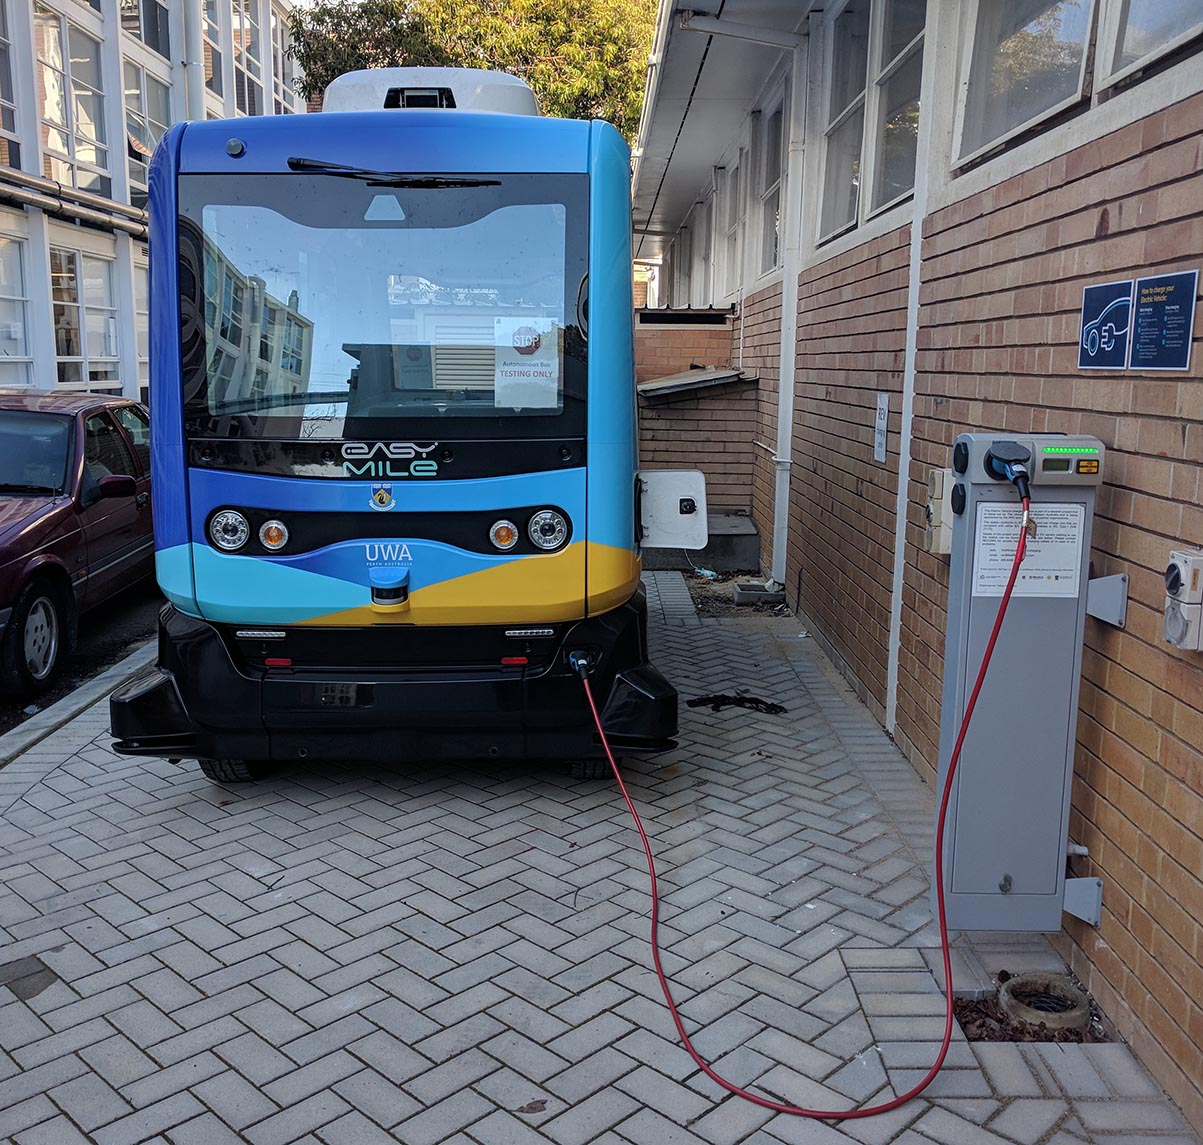
\includegraphics[width=0.6\textwidth]{bus}
	\caption{An EasyMile EZ10 driverless shuttle at a UWA charging station.}
	\label{fig:1:bus}
\end{figure}

\section{Autonomous Driving}
The general attainability of precise sensors and high performance compute hardware have driven recent interests in autonomous driving. Autonomous cars (also known as self-driving cars or driverless cars) perform autonomous driving by processing sensor data using an advanced control system that actively calculates the vehicle's navigation trajectory with obstacle avoidance. The sensors are often a combination of LiDARs, radars, sonar, GPS, local odometry, cameras and inertial measurement units (IMUs), which collectively compute through a process known as sensor fusion. Results from sensor fusion therefore enable the vehicle to achieve self-localisation or dead reckoning, along with scene understanding and object tracking. An example of an autonomous car is photographed in Fig.~\ref{fig:1:av}, showing its roof-mounted cameras and positioning sensors. 

\begin{figure}[ht] 
	\centering    
	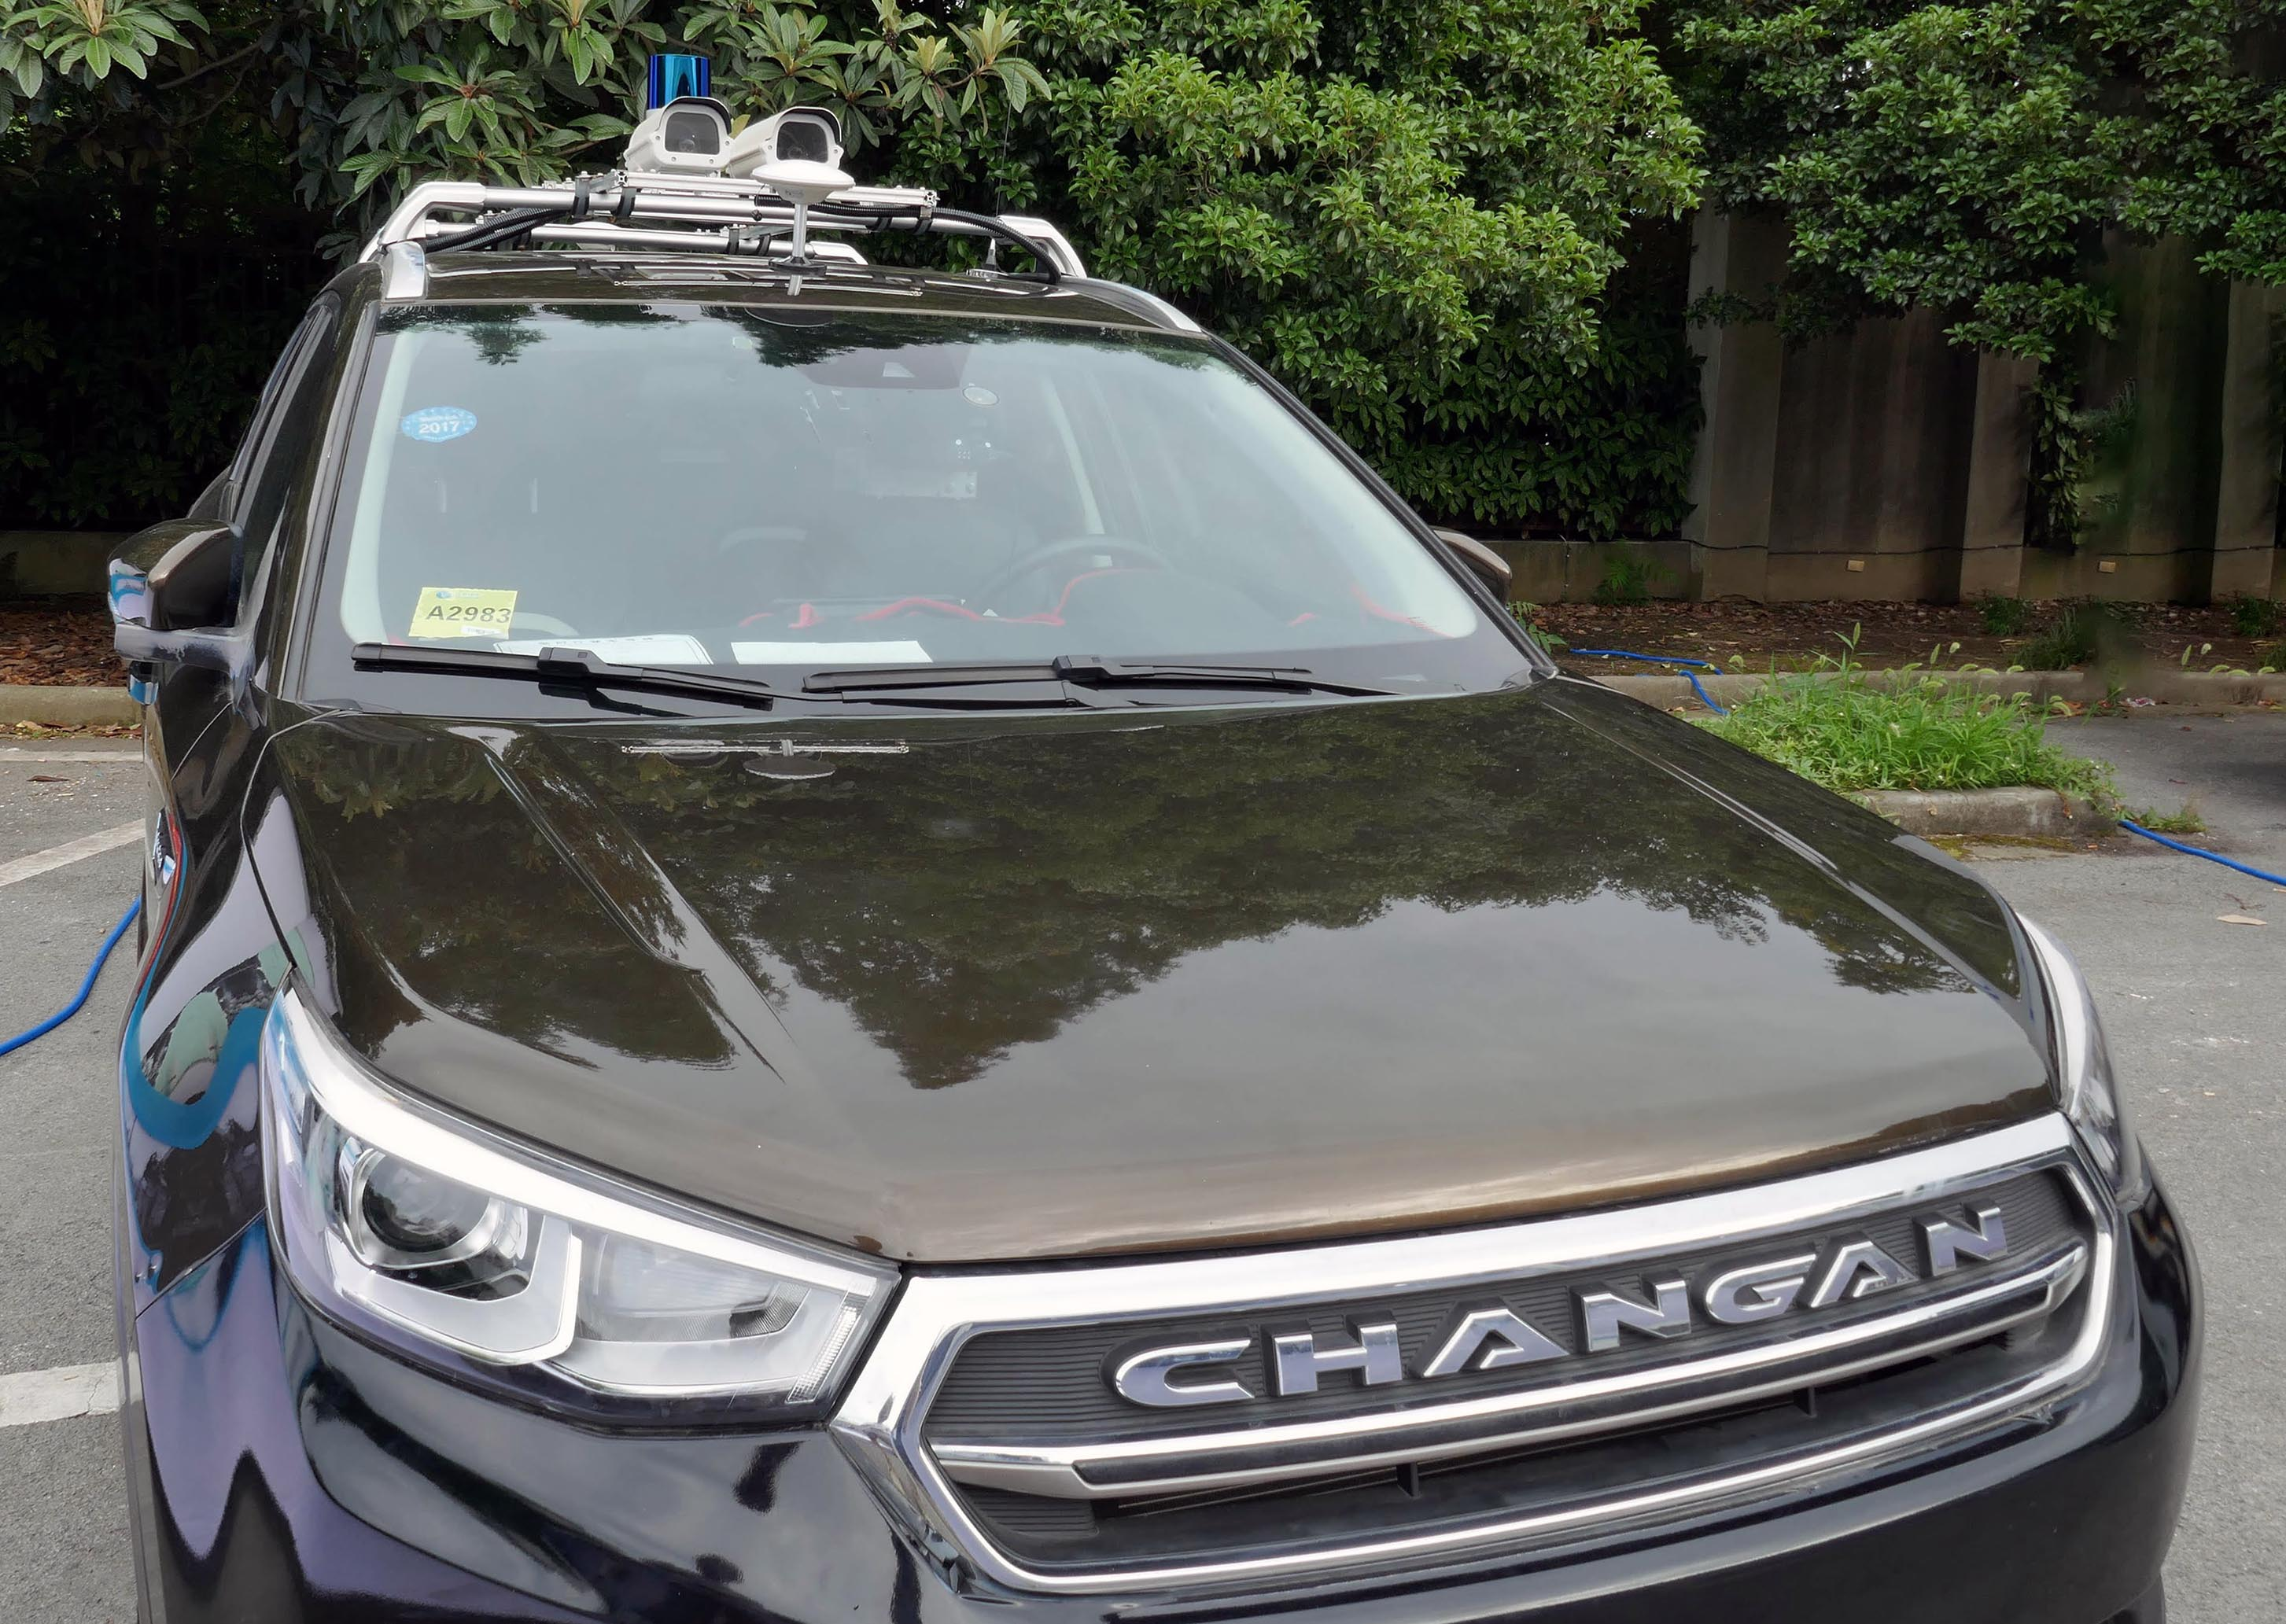
\includegraphics[width=0.7\textwidth]{av}
	\caption{An autonomous car with its sensors visibly mounted on its roof.}
	\label{fig:1:av}
\end{figure}

While autonomous cars have been developed as early as the 1980s~\cite{dickmanns_autonomous_1987}, many would argue that it was not until the DARPA Grand Challenge~\cite{buehler_2005_2007} before mainstream research into autonomous driving commenced. Since then, the developments in this area have been growing at a rapid pace. Market research reports published in 2018--2019~\cite{grand_view_research_self-driving_2018, kumar_autonomous_2018, htf_market_intelligence_overview_2019} have estimated the global capitalisation of autonomous vehicles to be valued at US\$55 billion in 2019, with a 35 per cent average compound annual growth rate (CAGR). Further, the Global Automotive \& Transportation Research Team at Frost \& Sullivan~\cite{frost_&_sullivan_global_2018} is expecting this figure to raise up to US\$173 billion by 2030, and also stated that shared mobility services such as ride-hailing are to contribute towards a 65 per cent share. 

Legislations pertaining to autonomous driving is also increasing in response to its growth. As of May 2019, according to the National Conference of State Legislatures (NCSL), 29 states in the United States have enacted autonomous vehicle legislations~\cite{hubbard_synthesis_2017}. The NCSL has also set up a publicly available Autonomous Vehicle State Bill Tracking Database that is easily searchable to cover various topics from commercialisation to vehicle testing~\cite{national_conference_of_state_legislatures_autonomous_2019}. In Australia, the National Transport Commission (NTC) has been tasked by the Australian Government to draft legislations relating to autonomous vehicles at the federal level~\cite{national_transport_commission_automated_2019}, including vehicle standards and safety concerns. This is performed while collaborating with various state governments, including Western Australia's Department of Transport~\cite{department_of_transport_automated_2018} to ensure nationwide consistency. %The REV Project at The University of Western Australia (UWA) actively participates 

%https://rosap.ntl.bts.gov/view/dot/35994s
%https://www.htfmarketreport.com/reports/1304659-global-self-driving-car-market-2
%https://www.mordorintelligence.com/industry-reports/autonomous-driverless-cars-market-potential-estimation
%https://www.grandviewresearch.com/industry-analysis/driverless-cars-market
%https://www.alliedmarketresearch.com/autonomous-vehicle-market

Safety is often a salient aspect of any successful development or legislation of autonomous vehicles. This landscape intends to minimise the human factor in driving, noting that human errors caused 94 per cent of all vehicle accidents in the United States~\cite{singh_critical_2015}, which would imply that an ideal autonomous vehicle penetration will reduce accidents by up to 90 per cent~\cite{bertoncello_ten_2015}. Similarly, 51 per cent of road fatalities in Australia are caused by the driver in 2018~\cite{department_of_infrastructure_transport_cities_and_regional_development_safety_2019}. In order to encourage the penetration and public perception towards autonomous vehicles, MIT's Technology Review has noted the lack of an industry standard for the safety of autonomous vehicles, and have published a brief report relating to the safety regulations~\cite{mit_technology_review_insights_autonomous_2019}. 

%https://crashstats.nhtsa.dot.gov/Api/Public/ViewPublication/812115
%https://www.bitre.gov.au/statistics/safety/

With the economics, legislation and safety setting the development baseline, autonomous driving applications have since evolved from advanced driver-assistance systems (ADAS), where it initially incorporated features including adaptive cruise control, automated parking, blind spot detection, lane departure warning, automatic lane centring and collision avoidance. Driving automation often consolidates these features with active navigation and control, minimising the need for driver intervention. To this end, SAE International has classified driving automation into five different levels under its J3016 ``Levels of Driving Automation'' standard, ranging from Level 0 (manual driving) to Level 5 (fully autonomous driving)~\cite{on-road_automated_driving_orad_committee_taxonomy_2018}. %SAE Report downloaded
The official SAE J2016 graphic is given as Fig.~\ref{fig:1:j3016}. An increase in driving automation level would typically require greater computation complexity, often using more sensors than its preceding level. Automotive manufacturers have begun the inclusion of Level 3 automation features in production vehicles since 2018, most notably with Tesla's Autopilot feature. 

\begin{figure}[H] 
	\centering    
	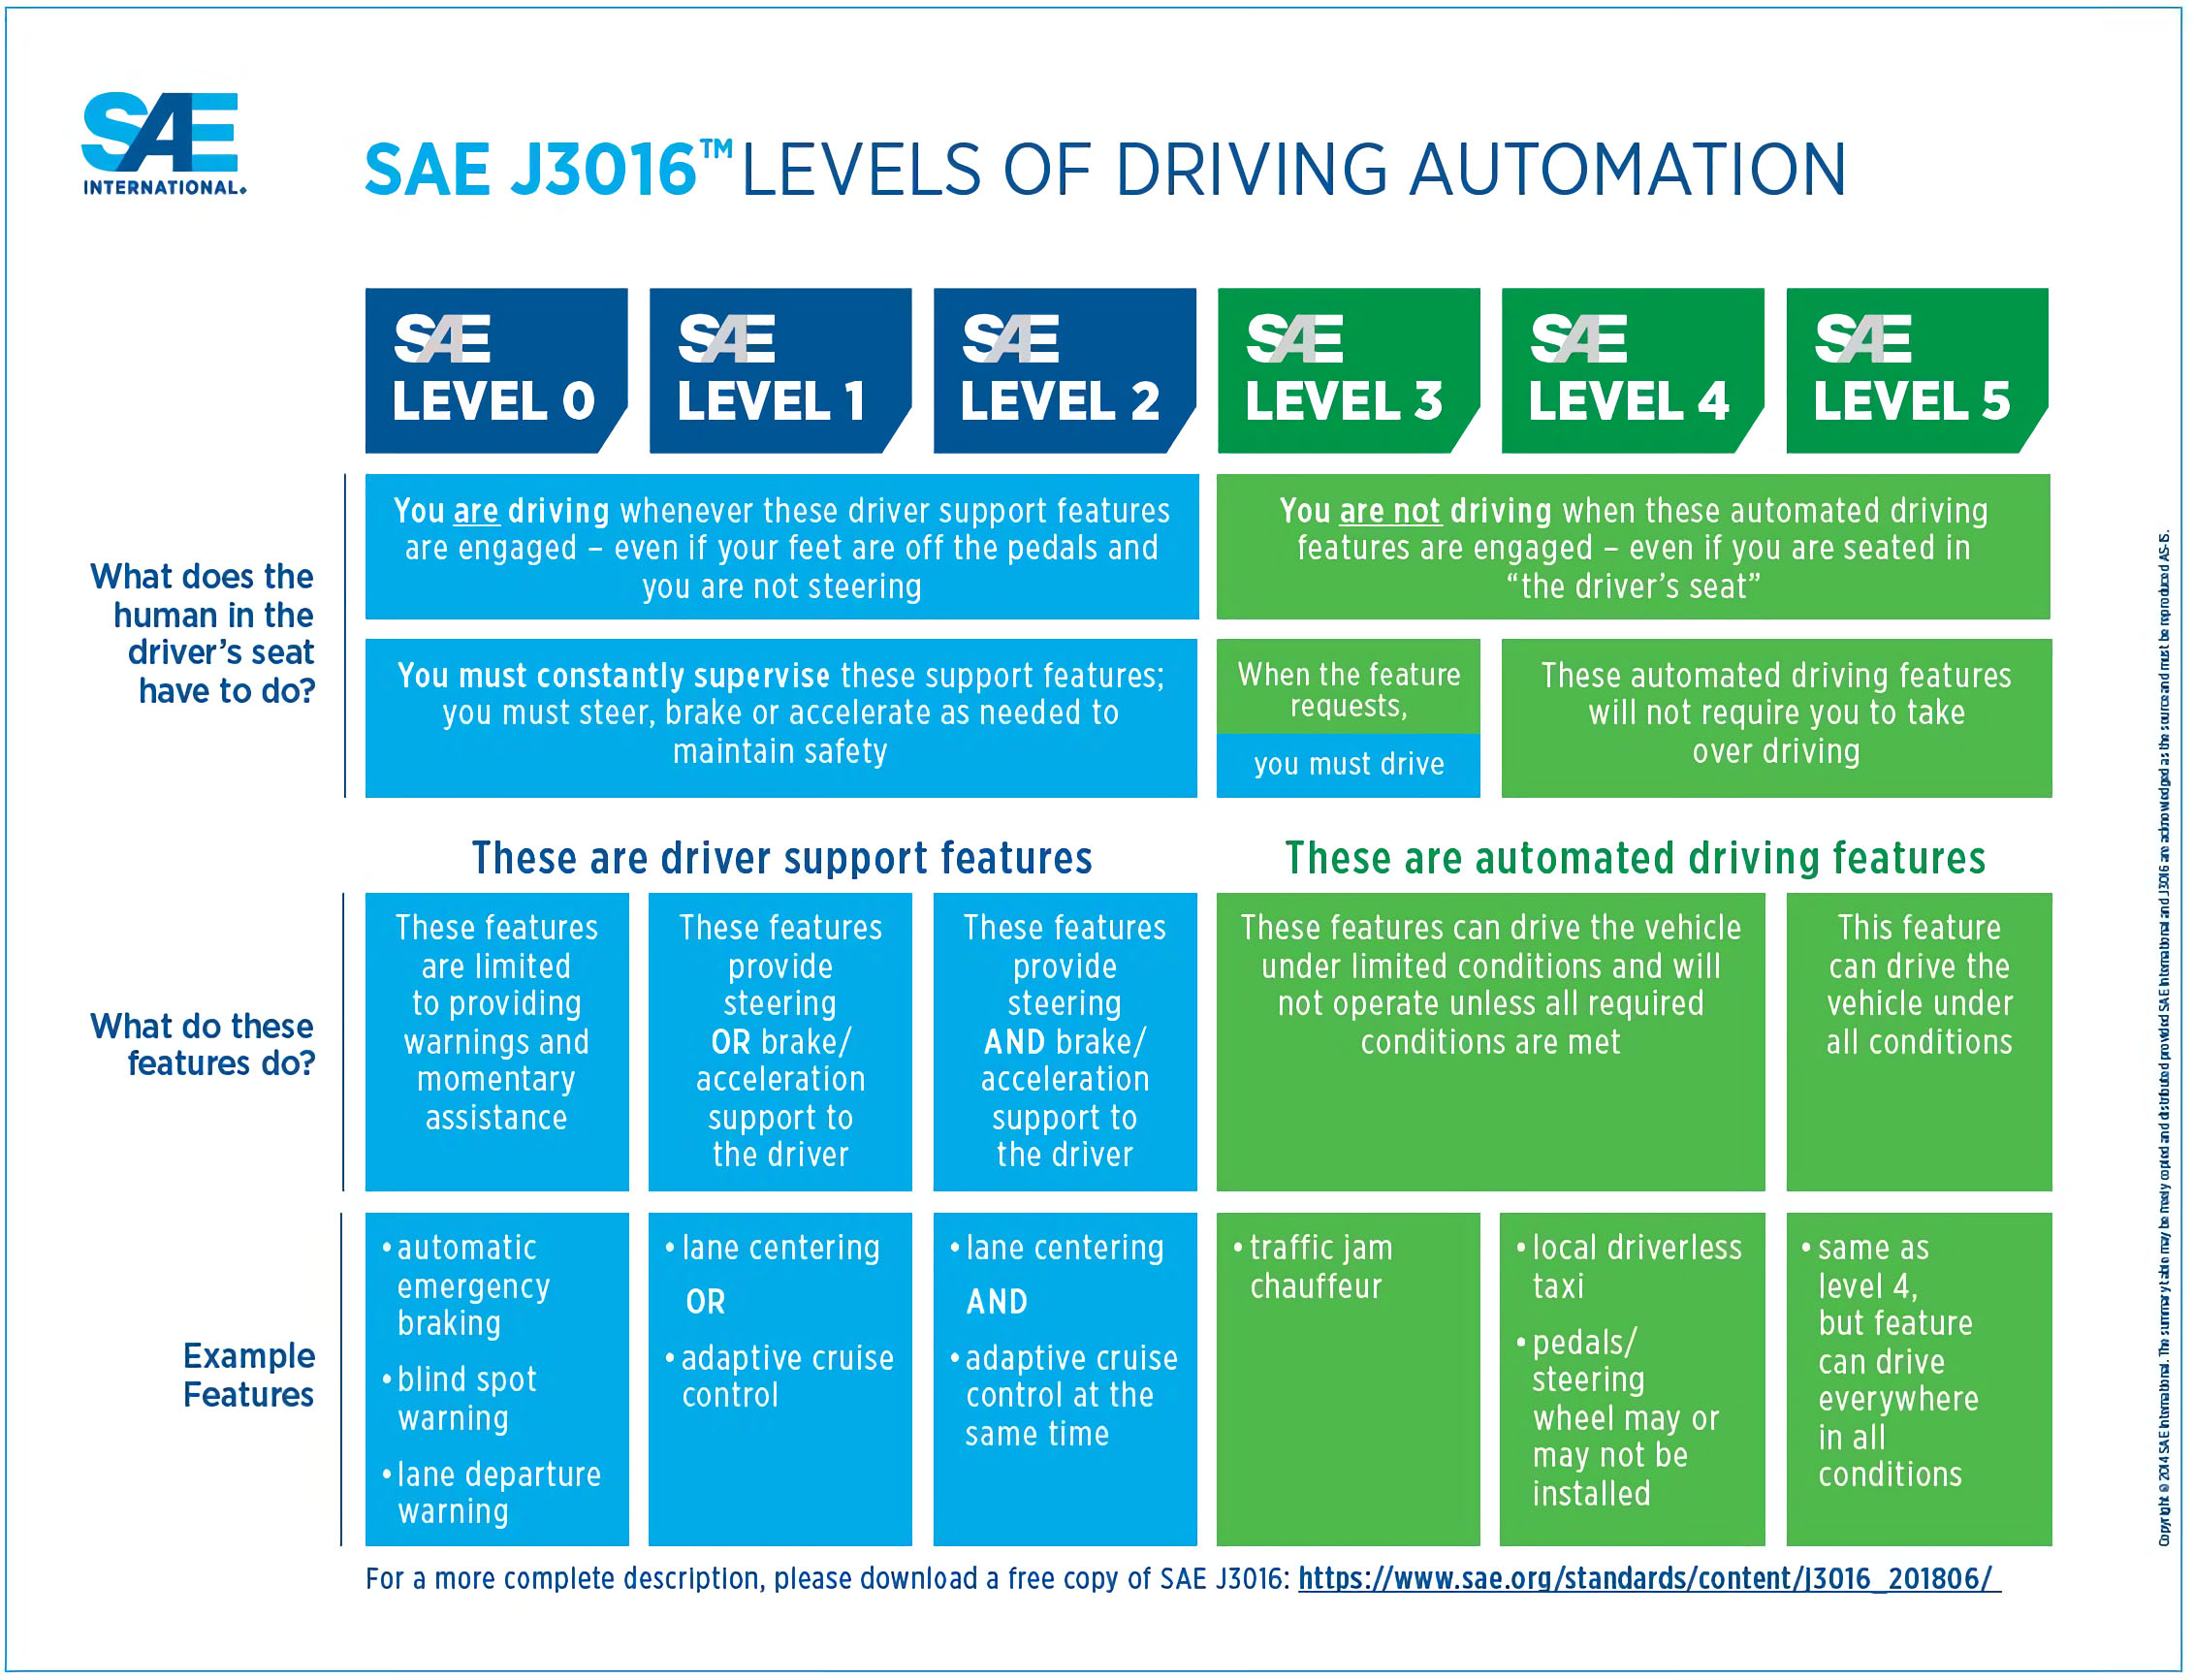
\includegraphics[width=\textwidth]{j3016}
	\caption[SAE J3016 official graphic]{The official graphic for the SAE J3016 standard as of January 2019~\cite{shuttleworth_sae_2019}.}
	\label{fig:1:j3016}
\end{figure}

Trials for Level 4 and 5 automation are being conducted by technological corporates such as Google (Waymo) and Uber. It is currently less favoured by production vehicles as the addition of high accuracy sensors would render the ownership cost prohibitive. In the case of positioning, conventional GPS devices have a reporting accuracy of approximately 10 metres, which is inadequate for autonomous navigation; many applications instead use differential GPS or real-time kinematic (RTK) to obtain accurate positioning, incurring higher implementation costs. On the perception front, vehicles often use LiDARs or radars to survey their immediate environment, thereby enabling them to detect or classify objects, and perform obstacle avoidance when necessary. LiDARs are typically preferred over radars in for object tracking and mapping, as it provides distance measurements accuracies in the order of millimetres. They are also capable of producing high definition maps, enabling precise localisation for the vehicles. These vehicles often install multiple LiDARs on their chassis to achieve a \ang{360} perception of its surroundings, often in addition to having dedicated LiDARs for mapping. This further increases the implementation costs, especially considering that individual LiDARs often cost tens of thousands of dollars. 

Due to the lower cost of cameras compared to LiDARs, newer applications are starting to favour using the camera as the vehicle's main perceptive sensor. These applications use computer vision methods to achieve localisation and object classification, often through a single input. However, computer vision algorithms are often more complex, requiring greater computation and memory footprints. This is particularly true when compared against LiDAR-based methods, as they only output a series of measurements, as opposed to a series of complete images that a camera outputs. Nevertheless, with the arrival of high-performance parallel computers, computer vision methods are more likely to better utilise these hardware platforms to achieve more desirable outcomes. These methods have been demonstrated to deliver results pertaining to accurate localisation, mapping and scene understanding; ideally replacing the need for LiDARs, radars, IMUs and local odometry. Using the cameras offer a more cognitive approach to autonomous driving, whereby it mimics a human's visual perception of the world while driving. Tesla has always maintained a critical position towards LiDARs and favouring the cameras due to its cost and due impracticality, with its CEO Elon Musk claiming that ``Anyone relying on LiDAR is doomed'', during his keynote address at the 2019 Tesla Autonomy Investor Day~\cite{burns_anyone_2019}.

This thesis describes works that contribute towards using the camera as the primary sensor for autonomous driving, viz. visual autonomous driving. By evaluating these algorithms on the testbed shown in Fig.~\ref{fig:1:sae}, it was found that algorithms relating to environmental perception and localisation can be substituted with computer vision methods. For instance, visual odometry is used in place of wheel odometry and inertial measurements; object classification, detection and tracking be done using the camera in place of LiDARs. Computer vision methods are therefore more versatile as multiple algorithms are able to leverage on a single data source. By doing so, these sensors can then supplement computer vision measurements as an alternative to improve upon classification or measurement accuracies. 

\begin{figure}[ht] 
	\centering    
	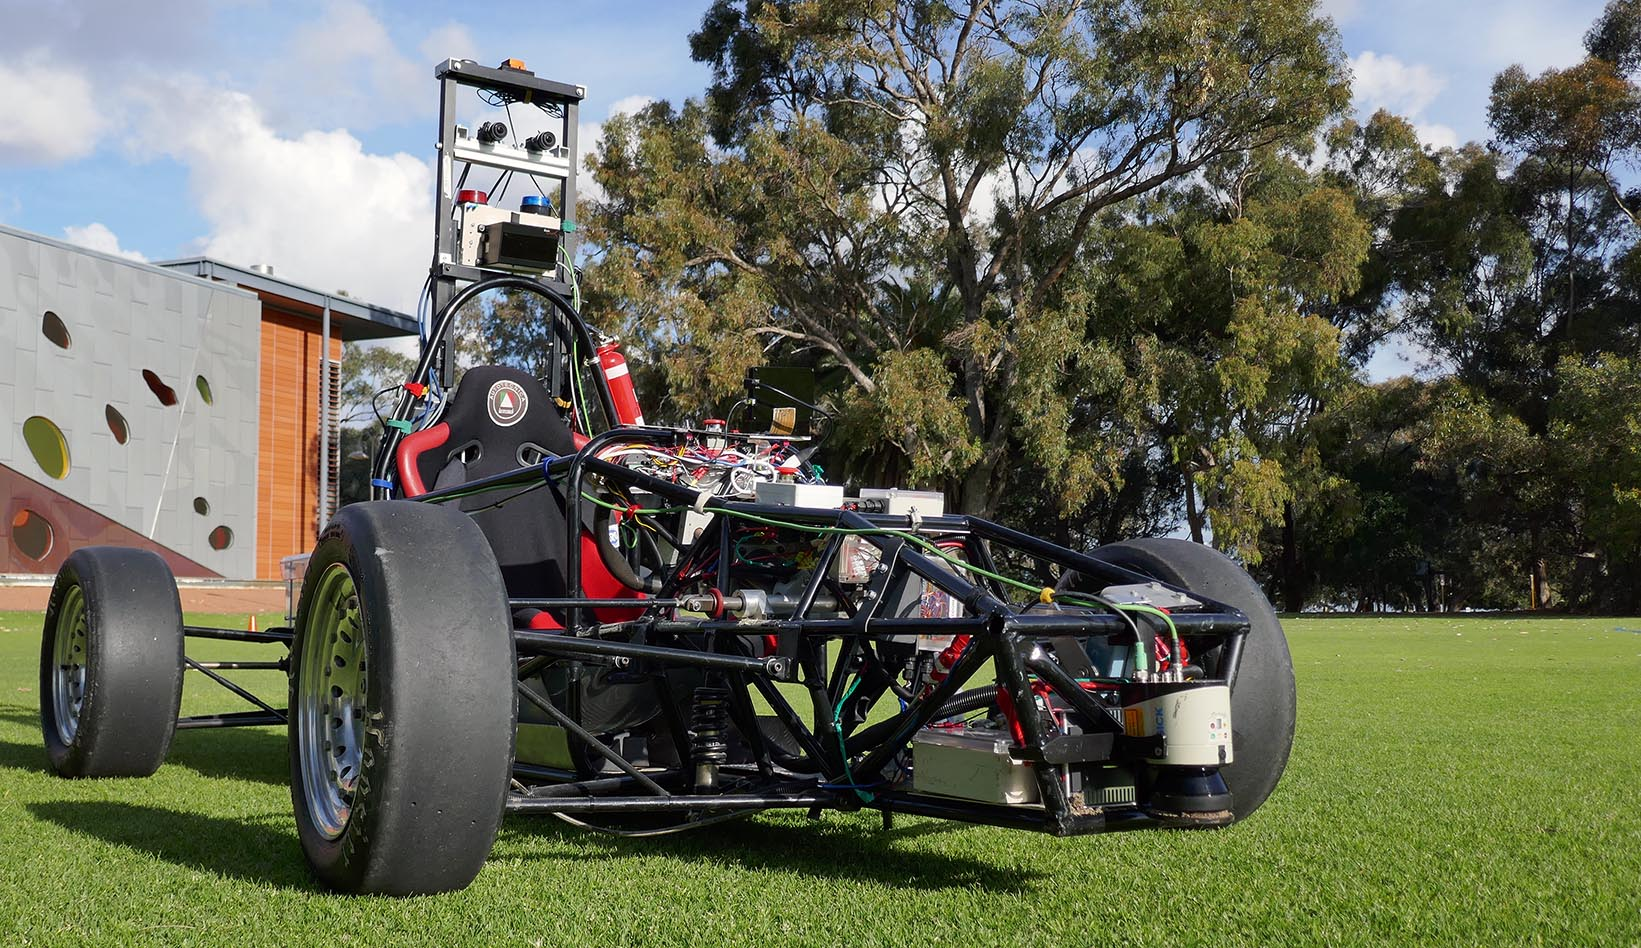
\includegraphics[width=0.7\textwidth]{sae}
	\caption{The REV Project's autonomous Formula SAE Electric test vehicle.}
	\label{fig:1:sae}
\end{figure}

\nomenclature[z-lidar]{LiDAR}{Light Detection and Ranging} 
\nomenclature[z-gps]{GPS}{Global Positioning System} 
\nomenclature[z-imu]{IMU}{Inertial measurement unit} 
\nomenclature[z-cagr]{CAGR}{Compound annual growth rate} 
\nomenclature[z-ncsl]{NCSL}{National Conference of State Legislatures} 
\nomenclature[z-darpa]{DARPA}{Defense Advance Research Projects Agency} 
\nomenclature[z-adas]{ADAS}{Advanced driver-assistance systems} 
\nomenclature[z-rtk]{RTK}{Real-time kinematic (positioning)} 


%history, OEMs, safety, levels SAE, future applications
\section{Electromobility}
The increased awareness of climate change at the turn of the century is contributing to the rise in sustainable and renewable energy sources worldwide. Heightened levels of greenhouse gas emissions have prompted international treaties, most notably the United Nations Framework Convention on Climate Change (UNFCCC). The UNFCCC Paris Agreement saw 195 ratifications to tackle issues relating to global warming, with a focus to reduce greenhouse gas emissions, and to increase the share of renewable energy and energy efficiency, limiting warming to under 1.5--2°C~\cite{rogelj_paris_2016}. This agreement came into force on 4 November 2016. Carbon dioxide (CO\textsubscript{2}) remains by far the largest contributor to greenhouse gas emissions (82 per cent)~\cite{united_states_environmental_protection_agency_inventory_2019}. In part, transport is responsible for 23 per cent of global emissions, and is projected to increase to 50 per cent by 2050; car emissions constitute half of this figure~\cite{santos_road_2017}. In Australia, transport remains the second largest source of greenhouse gas in the country, emitting 102 million tonnes (18 per cent) of CO\textsubscript{2} in 2018, and is projected to reach 111 million tonnes by 2030 at its current rate~\cite{department_of_the_environment_and_energy_australias_2018}. 

%https://unfccc.int/resource/docs/2015/cop21/eng/l09r01.pdf
%https://www.epa.gov/ghgemissions/inventory-us-greenhouse-gas-emissions-and-sinks
%https://www.sciencedirect.com/science/article/pii/S0967070X17304262
%https://www.environment.gov.au/system/files/resources/128ae060-ac07-4874-857e-dced2ca22347/files/australias-emissions-projections-2018.pdf

Noting that a vehicle's CO\textsubscript{2} emissions increases with its fuel consumption and type, the automotive industry is making efforts to reduce the carbon footprint of production vehicles with the introduction of green vehicles that run on alternative fuels, including electricity. Electromobility (or e-mobility) is a portmanteau of electric and mobility that is often used to describe electric driving in light of its renaissance that began in the late 2000s. Since the late 2010s, it is mainly used to describe electric vehicles (EVs), particularly electric cars as a relation to current motoring trends.

Electromobility was first conceptualised in the 1900s, back when climate change was unlikely to be a concern. The rationale to produce electric cars back then was to mitigate rising fossil fuel prices while being less noisy. However, it was quickly phased out of favour due to subsequent advancements with the internal combustion engine (ICE)~\cite{kirsch_electric_2000}. Still, the availability and know-hows in electromobility continued to persist and improve over the years with overhead line-based transportation, and components such as motors and controllers have become faster and more efficient. Throughout the century, several attempts have been made to reintroduce electric driving to the market, more recently with the General Motors EV1~\cite{johnson_environmental_1999}, but inadequate battery technologies and slow charging speeds have restricted their market penetration. These cars often use lead- and nickel-based batteries which are often heavy and have lower energy densities that are insufficient to sustain a suitable driving range.

The electromobility resurgence in the late 2000s was catalysed by climate change awareness and government incentives. This began with the introduction of hybrid electric-petroleum vehicles as a compromise between low tailpipe emissions and a limited electric range, as the batteries can be charged off its engine, ceding its reliance on charging stations. With the push towards zero tailpipe emissions by government lobbyists with additional incentives, automotive manufacturers have begun producing plug-in hybrid and battery EVs that mainly run on electric motors. Around the same time, the proliferation of lithium-ion batteries in personal electronic devices has benefited from improved affordability and energy density, to which these are adopted by EVs~\cite{hannan_review_2017}. Using lithium-ion cells introduces longer ranges and high speed charging to the vehicle, which is in line with current electromobility trends. Another energy storage that is gaining attention with EVs is the hydrogen fuel cell, which uses a redox reaction to generate electricity. These vehicles do not need to be charged, but rather rely on hydrogen as fuel, which requires them to be filled up at hydrogen filling stations. This requires hydrogen to be processed (often through electrolysis), transported and stored multiple times throughout its production chain, constituting to high energy usages and emissions that are three times higher than a battery EV~\cite{smit_where_2018} even before it can be used as vehicle fuel. This is in addition to safety concerns during transport as hydrogen is highly flammable. This is in contrast to rechargeable batteries that can easily be charged off the grid.

The charging of EVs can occur at a standard electrical outlet, or at EV charging stations (see Fig.~\ref{fig:1:cs}) which are capable of delivering faster charges, and can be installed in public or private car parks or garages. Charging station deployments are actively effectuated, often by local public authorities and corporate enterprises, especially in developed countries. PlugShare~\cite{plugshare_plugshare_nodate} is a website that maps charging station locations through crowdsourcing, and currently tracks them in more than 112,000 locations worldwide with at least 170,000 outlets. Many of these stations belong to a charging station network, which is a collective system of charging stations owned or managed by governments, automotive companies or charging station manufacturers; a notable example is the Tesla Supercharger~\cite{tesla_supercharger_nodate} network. Many networks are capable of connecting to the Internet, which enables usage monitoring and tracking for station users and administrators. Connected charging infrastructures such as these are often also capable of facilitating smart charging or vehicle-to-grid (V2G) systems. 

\begin{figure}[ht]
	\centering
	\begin{subfigure}[b]{0.45\textwidth}
		\centering
		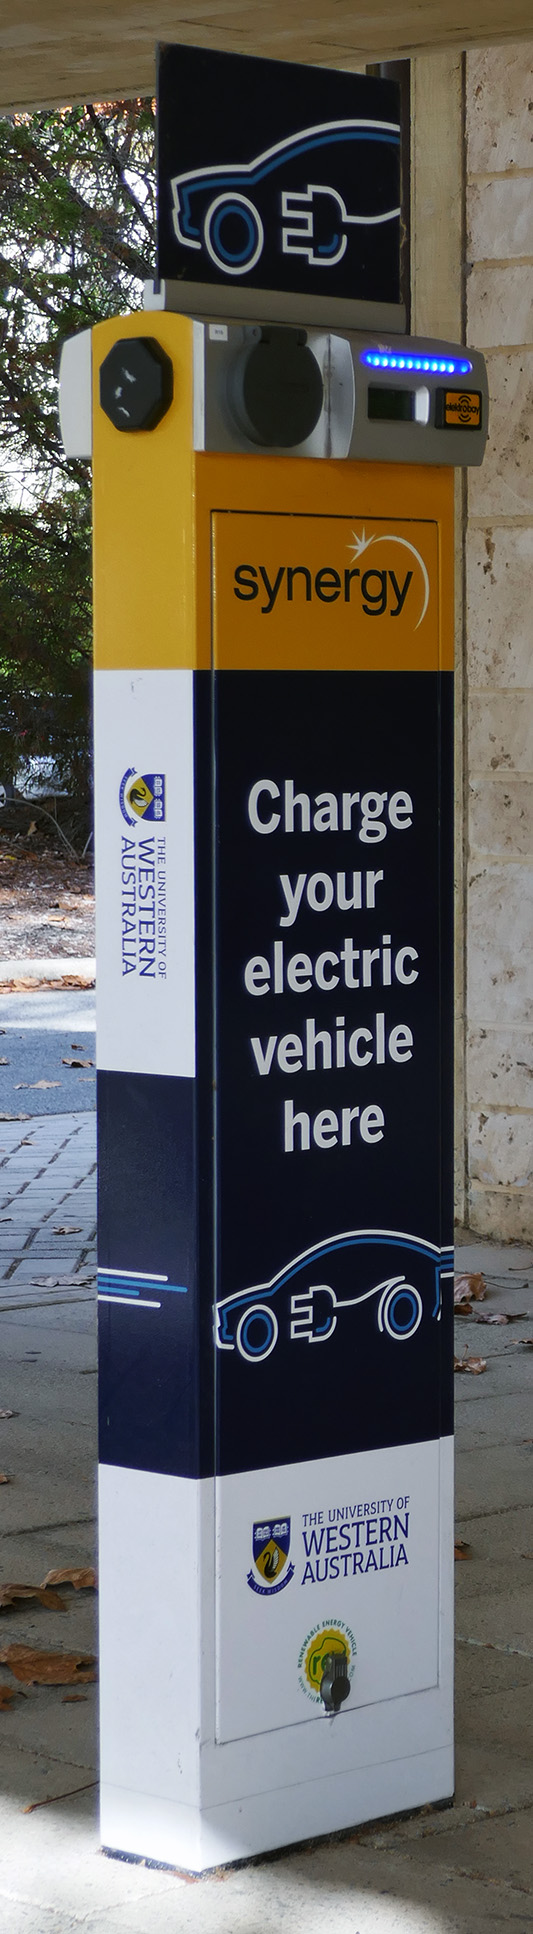
\includegraphics[height=7cm]{accs}
		\caption{AC Charging Station}
		\label{fig:1:accs}   
	\end{subfigure} 
	\hspace{1em}         
	\begin{subfigure}[b]{0.45\textwidth}
		\centering
		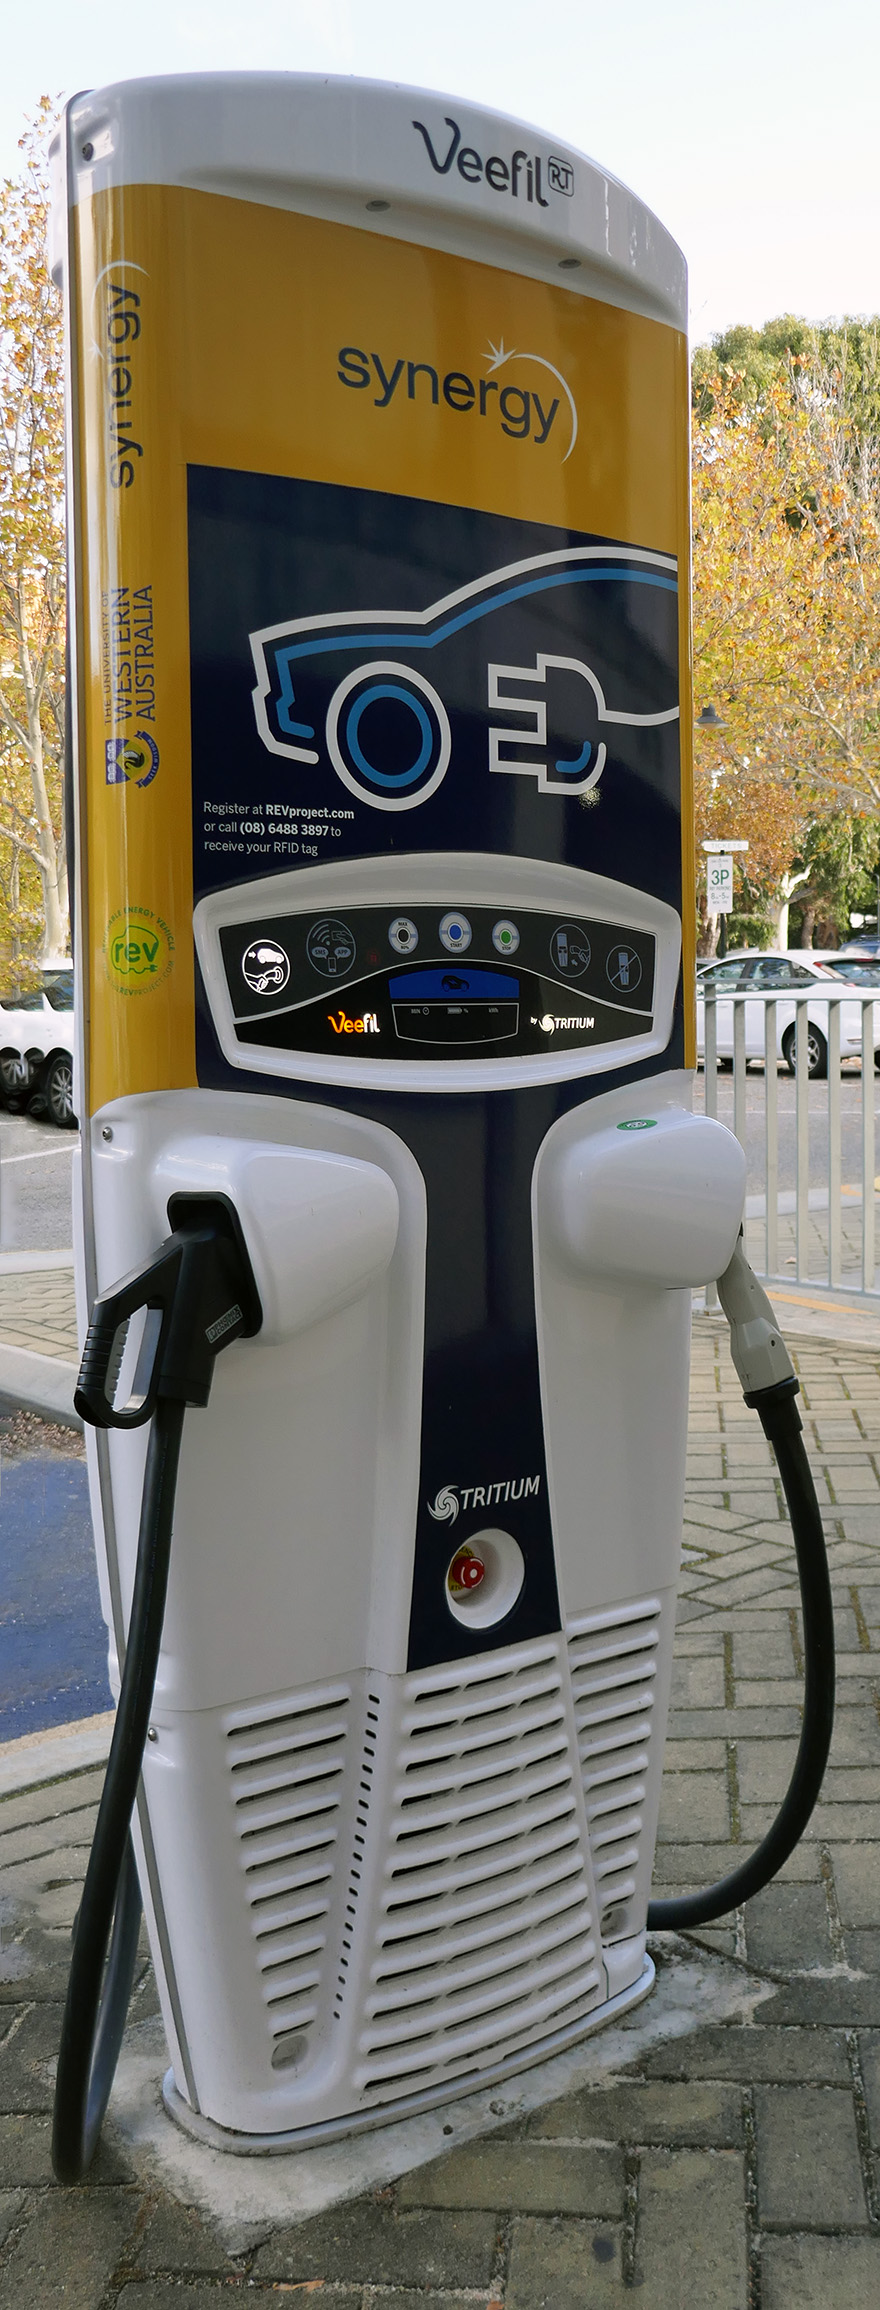
\includegraphics[height=7cm]{dccs}
		\caption{DC Charging Station}
		\label{fig:1:dccs}
	\end{subfigure}             
	\caption{UWA's AC and DC charging stations.}
	\label{fig:1:cs}
\end{figure}

Regulations and incentives have been drafted across various countries either in preparations or in attempts to stimulate EV penetration due to increasing benefits beyond its carbon footprint. These benefits include the running cost of the vehicle, as~\cite{joseph_how_2016} has calculated that an average EV (18 kWh/100 km) is up to five times cheaper to run per kilometre than a typical ICE vehicle (11.1 L/100 km), and are up to 90 per cent more energy efficient. Noting the higher initial cost of EV ownership, many countries have incentivised EV uptakes across varying degrees~\cite{broadbent_electric_2018}. Compared to successful initiatives such as in Norway~\cite{bauer_impact_2018}, the consumer acceptance of EVs is still low in Australia, and researches to encourage local EV uptakes have been limited~\cite{broadbent_analysis_2019}. Notwithstanding, the Australian Senate has established a Select Committee on Electric Vehicles to investigate this issue, resulting in a table of a report~\cite{senate_select_committee_on_electric_vehicles_report_2019}. The notable recommendations presented in this report include a development of national strategy for EVs and charging infrastructures, and setting up a national EV target. Researches in these areas will likely expedite the implementations of the recommendations. 

%https://www.mdpi.com/2032-6653/10/1/11/htm#B2-wevj-10-00011
%https://onlinelibrary.wiley.com/doi/full/10.1111/gec3.12358
%https://www.ergon.com.au/network/smarter-energy/electric-vehicles/charging-your-electric-vehicle

This thesis presents works that address this area through a quantitative analysis of EV charging behaviours using data that was collected from charging stations around Perth. Comparisons are drawn across different charging station types, taking into account a variety of usage scenarios to better visualise the current EV landscape, where it can be used to supplement policy roadmaps to encourage uptake.  
%incentives

\nomenclature[z-unfccc]{UNFCCC}{United Nations Framework Convention on Climate Change} 
\nomenclature[z-ice]{ICE}{Internal combustion engine} 
\nomenclature[z-ev]{EV}{Electric vehicle} 
\nomenclature[z-v2g]{V2G}{Vehicle-to-grid}
\nomenclature[z-iot]{IoT}{Internet of things}

\section{Connected Mobility}
With the availability of low-cost GPS tracking, fleet operators have often relied on vehicle tracking systems to remotely manage and monitor fleets of vehicles. Modern tracking devices are capable of Internet connectivity to transmit telemetry data to a centralised remote server. In addition to location information, this data can include diagnostics from various sensors on the vehicle. In the case of EVs, this can include battery and charging information. 

Further advancements in vehicular communications have incited this to evolve as part of the efforts in vehicle-to-everything (V2X) communications. V2X covers vehicular communication across several aspects including but not limited to V2I (vehicle-to-infrastructure), V2V (vehicle-to-vehicle), V2C (vehicle-to-cloud) and V2G (vehicle-to-grid)~\cite{pearre_review_2019}. These technologies often communicate through a wired or wireless network over a machine to machine (M2M) channel. In the case of wireless connectivity, mobile networks such as 4G are often favoured due to its high transmission speeds, with the incoming 5G standard likely being favoured upon mass deployment, as optimisations are present to facilitate this application. Using mobile networks for V2X applications is often referred to as cellular V2X (C-V2X)~\cite{papathanassiou_cellular_2017}.

With the advent of cloud and edge computing and the Internet of things (IoT), applications pertaining to V2C communications are becoming increasingly prominent, which include the works described in this thesis. V2C has specifically evolved from fleet management systems whereby the addition of a cloud infrastructure presents the application with intelligent control and monitoring~\cite{deng_cooperative_2019}. In the case of an EV ecosystem, a V2C system is capable of consolidating data relating to the EV, charging infrastructures, user behaviours and other stakeholders to present a unified framework for the entire ecosystem. This establishes part of the foundation that leads to intelligent transportation in a smart city, where data from the driving ecosystem is mutually shared for traffic and grid optimisation with low latency connectivity~\cite{hensher_tackling_2018, khattak_toward_2019}, setting the foundation for the Internet of vehicles (IoV).

These communication technologies are easily incorporated into intelligent transportation systems (ITS) to result in smart traffic management and planning; autonomous vehicles will be able to drive cooperatively using a collective perception similar to multi-agent or swarm robotics system. Automotive manufacturers have begun producing vehicles with limited connectivity, but market researches have predicted this market to expand by 45 per cent by 2020 with a 19 per cent CAGR~\cite{market_research_future_connected_2019}. These implications have not gone unnoticed by governments. In Australia, the governments of Western Australia~\cite{weeratunga_connected_2015} and New South Wales~\cite{transport_for_nsw_connected_2018} have studied and produced reports relating to connected vehicles, and the Queensland Government's Cooperative and Automated Vehicle Initiative (CAVI)~\cite{queensland_government_cavi:_2017} has been established to devise policies pertaining to this matter. 

Part of the work described in this thesis intends to establish some preliminary research into connected vehicles in Western Australia. It describes a cloud platform that aggregates data from edge computing that is delivered through a network of smart EV charging stations and an EV fleet. This performs according to a V2C and infrastructure-to-cloud communications system, thereby facilitating data management and reporting to deliver results relating to diagnostics, monitoring and usage forecasts. It is also configured to be extensible to account for the exponential growth in vehicular and infrastructure data, serving as a pragmatic entry into forthcoming big data researches. 

\nomenclature[z-iov]{IoV}{Internet of vehicles} 
\nomenclature[z-m2m]{M2M}{Machine to machine} 
\nomenclature[z-v2x]{V2X}{Vehicle-to-everything} 
\nomenclature[z-v2c]{V2C}{Vehicle-to-cloud} 
\nomenclature[z-v2v]{V2V}{Vehicle-to-vehicle} 
\nomenclature[z-v2x]{V2I}{Vehicle-to-infrastructure} 
\nomenclature[z-v2x]{V2X}{Vehicle-to-everything} 
\nomenclature[z-cavi]{CAVI}{Cooperative and Automated Vehicle Initiative} 
\nomenclature[z-cv2x]{C-V2X}{Cellular vehicle-to-everything} 
\nomenclature[z-4g]{4G}{Fourth generation} 
\nomenclature[z-5g]{5G}{Fifth generation} 

%An example of autonomous driving benefiting from V2V connectivity is through cooperative autonomous driving. This enables a group of vehicles to establish a collective perception, similar to multi agent or swarm robotics systems. 

%The adoption of high-speed wireless connectivity will also benefit autonomous driving, whereby driving decisions and routines including deep learning can be offloaded to a centralised cloud server for processing~\cite{}; traffic management systems can utilise the cloud to achieve adaptive real time performances~\cite{}.

%https://www.sciencedirect.com/science/article/pii/S0967070X17308867
%https://www.mainroads.wa.gov.au/Documents/Connect%20Vehicles%20Web.RCN-D15%5E23413758.PDF
%https://www.future.transport.nsw.gov.au/sites/default/files/media/documents/2019/Connected_and_Automated_Vehicles_Plan.pdf
%https://ieeexplore.ieee.org/abstract/document/8671732
%https://www.marketresearchfuture.com/reports/connected-mobility-solutions-market-871

%With regards to charging speeds, SAE International has published and classified this according to three levels, which Australia follows: 
%
%\begin{itemize}
%	\item Level 1: 2.4 kW AC charging with standard electrical outlets. A full charge is done overnight.
%	\item Level 2: 7.6 kW three-phase AC charging. Three to six hours for a full charge.
%	\item Level 3: Fast DC charging greater than 25 kW. A 350 kW charger typically charges a car in under 10 minutes. 
%\end{itemize}



%li ion fast charging

%paris agreement
%policies
%challenges in area, current state of art, fuel cell
%research question, aims, objective, motivation

%\section{Research Scope}
%This thesis presents its research scope as defined in its aim and objectives. It is multidisciplinary whereby cohesion is given under the context of autonomous electric vehicle applications. 
%
%\subsection{Aim}
%The series of works presented in this thesis aims to formulate pragmatic solutions pertaining to the navigation and charging of electric vehicles by answering the following research questions:
%\begin{enumerate}
%	\item Can autonomous driving be performed using the camera as the primary perceptive sensor?
%	\item How can data from EVs and charging infrastructures be interpreted in a meaningful way?
%\end{enumerate}

\section{Contributions}
The series of works presented in this thesis aims to formulate pragmatic solutions pertaining to the camera as the main sensor for autonomous driving, and interpreting data from EVs and charging infrastructures in a meaningful way. It is multidisciplinary whereby cohesion is ensured under the context of designing system frameworks for autonomous electric vehicle applications. 

To this end, the main contributions of this thesis are summarised as follows:
\begin{itemize}
	\item A literature survey pertaining to visual road recognition with specific emphasises on the methods for autonomous driving applications. Learning methods are presented against conventional methods; recent works relating to academia and the industry are discussed. [Chapter~\ref{ch:vrreview}]
	\item A literature survey pertaining to visual odometry with specific emphasises on autonomous driving applications. These are categorised according to the types of camera used in relation to the current state of research. [Chapter~\ref{ch:voreview}]
	\item An incorporation of visual odometry and semantic segmentation into a multi-robot system. This introduces visual navigation onto an existing system to improve odometric accuracies, and to enable scene understanding for dynamic object recognition. [Chapter~\ref{ch:cmrn}]
	\item An implementation of semantic segmentation on a physical LiDAR-based autonomous driving testbed. This proposed method uses a low-cost monocular camera to segment road regions and lane markings for road centring. [Chapter~\ref{ch:semseg}]
	\item An autonomous driving software framework that is modularly unified to interface sensors with control modules independently. This framework uses protocol buffers to streamline module interoperability to provide an optimised compute performance. [Chapter~\ref{ch:modular}]
	\item A hybrid extension to the aforementioned software framework using Robot Operating System (ROS). Algorithmic additions to path planning and visual navigation are included, along with sensor interfaces and safety functionalities. [Chapter~\ref{ch:evo}]
	\item A hardware-in-the-loop (HIL) simulation system for autonomous driving without real-time constraints. The compute hardware is identical to that used on the autonomous driving testbed using the same ROS integration. [Chapter~\ref{ch:sim}]
	\item A web-based software framework for electromobility telematics. It aggregates and curates data from connected vehicles, charging infrastructures and energy sources, interpreting it for meaningful real-time monitoring and visualisation. [Chapter~\ref{ch:review}]
	\item An analysis of EV charging behaviours on charging stations in Western Australia. Comparisons are drawn across the types and locations of charging stations for their adoption rate, and cost model presented subsequently. [Chapter~\ref{ch:charging}]
\end{itemize}

\nomenclature[z-ros]{ROS}{Robot Operating System} 
\nomenclature[z-hil]{HIL}{Hardware-in-the-loop} 

\section{Thesis Outline}
This thesis comprises of 11 chapters, wherein two chapters present on background reviews, five on autonomous driving frameworks or methods and two on electromobility telematics. The 10 chapters that are subsequent to this introductory chapter are structured as follows: 
%2 survey chapters, 3 on autonomous nav, 2 on electromonbility analysis
\begin{description}
	\item[Chapter~\ref{ch:vrreview}] presents a survey into the current state of research on methods for computer vision-based road recognition. The backgrounds into the methods are first presented categorically according to conventional (non-learning) and machine learning methods, followed by the implementations of these methods. Conventional methods are presented structurally, following common implementations including horizon and vanishing point detection, region of interest isolation, image classification and model fitting; machine learning methods relate to support vector machines and deep learning approaches, covering popular datasets and image segmentation algorithms. These methods are further reviewed for their implementations in relation to autonomous driving. This is presented first as commercial implementations, covering works from corporates and startups, before presenting on recent academic works with practical implementations. 
	\item[Chapter~\ref{ch:voreview}] presents a review on visual odometry methods for autonomous driving across three approaches --- monocular, stereoscopic and visual-inertial. Related applications are discussed for each approach, focusing on works with practical implementations. This is followed by tables that summarise the methods and their presented applications with any applicable datasets. A discussion is drawn to analyse the practicality of the works presented, emphasising on their viability for autonomous driving applications. Through this review it was known that many works truncate upon experimental validations on datasets, and never proceeded with a tangible implementation, leading to a scarcity in their implementations for autonomous vehicles. This chapter concludes by drawing the necessity of such implementations, as the dynamism of real-world environments must be accounted for.
	\item[Chapter~\ref{ch:cmrn}] describes an implementation of visual odometry and semantic segmentation onto a multi-robot system. The proposal of this implementation acts as a preliminary testbed for the visual navigation algorithms to test their application feasibility before they are ported onto an actual road vehicle. In addition, the incorporation of these algorithms intends to improve upon the existing multi-robot system's localisation accuracy, as well as supplementing navigation with scene understanding. In particular, as the existing system localises upon wheel odometry, the introduction of visual odometry intends to mitigate the error accumulation caused by wheel slip, a common problem that occurs in wheel odometry systems. Navigation on the system is performed in a decentralised manner, such that navigational algorithms run independently on each robot without relying on an external or central computer. Evaluations on the visual navigation algorithms have ascertained the feasibility of their implementations in solving problems relating to odometry and object classification while being resilient against environmental dynamics. 
	\item [Chapter~\ref{ch:semseg}] focuses on the application of a semantic segmentation method onto an autonomous driving testbed. The existing testbed is equipped with a LiDAR for object detection, and the addition of visual navigation intends to supersede that to achieve scene understanding and object perceptibility. A low-cost USB camera is mounted onto the vehicle's frame, where it and the other sensors are physically calibrated for camera-LiDAR distance measurements. Semantic segmentation is then applied to the camera recordings and its pixel accuracy is subsequently measured. Experimental results have shown that segmentation is adequate for road markings and lane detection on Perth roads. 
	\item [Chapter~\ref{ch:modular}] explores the first iteration for an improved software framework for the autonomous driving testbed. The original framework heavily relied on a central Control module which required all sensors and submodules to run. The proposed framework is more efficient whereby it is programmed using a C++ interface across all modules. Existing modules are either translated or reprogrammed, which streamlines and optimises individual algorithms to run on the testbed's embedded computer, enabling high performances throughout the software architecture. Module interoperability is ensured using protocol buffers, which separate them into independent classes. Experimental results have validated the efficiency of the software framework, which is given in outputs relating to localisation, odometry, path planning, control and semantic segmentation. 
	\item [Chapter~\ref{ch:evo}] proposes a hybrid enhancement to the C++-based software framework as a high-level control system. This new framework is based on ROS, and modularly combines sensor data and navigation processing for autonomous driving, while simultaneously ensures vehicle safety and provides data visualisation. %The navigation sensors achieve of wheel odometry, dead reckoning, LiDAR and camera detection
	It is capable of navigating along with a set of predefined waypoints, or along a cone-delimited path. Visual navigation is once again presented for road and lane detection using semantic segmentation, visual odometry and cone tracking. A HIL simulator is also presented to introduce a parallel development platform using identical compute hardware. Experiments were conducted for sensor fusion, waypoint driving, cone driving and the simulator, where results have collectively demonstrated the system's robustness and adequacy for practical implementations. 
	\item [Chapter~\ref{ch:sim}] expands on the HIL simulation system described to elaborate on its features. Using a HIL system enables algorithmic prototyping to be rapidly deployed while reducing such risks when compared to a physical system. This is a CARLA-based simulation system at the front-end, whereas autonomous driving routines are performed using identical ROS-based compute hardware across real-world and simulation testbeds to illustrate realistic constraints in relation to its computation footprint. This include using identical ROS modules for LiDAR point clouds and camera visualisations. Comparisons were made between the simulation and the physical system, with articulations on the cone detection (LiDAR and vision-based) and path planning algorithms. Evaluations were drawn to benchmark these algorithms, in addition to vehicle dynamics and computation requirements, where it was verified that the tests conducted are transferable between physical and simulation systems.
	\item [Chapter~\ref{ch:review}] introduces the electromobility research in this thesis by detailing the software framework used to collect and process telemetry data from various EVs and their infrastructures. A centralised cloud server is developed for this telematics platform which EVs, charging infrastructures and power sources push data to. The application layer is entirely web-based and is capable of pulling data in real-time for user monitoring and visualisations. This is presented for charging stations, EV fleet tracking and energy generation, wherein for each section, the back-ends and algorithms are elaborated to result in visualisations. Gamification is presented for vehicle tracking to encourage economical driving, and monetisation options are presented as bills to inform users of energy usage in charging stations. The results generated from this telematics platform were summarised as usages pertaining to charging infrastructures and energy generation, as well as heat maps for EV tracking. A forecast of the charging infrastructures' usage is also presented and analysed as a precursor to predicting the local EV penetration. All platform modules were written in a modular approach to encourage future improvements and expansions.  
	\item [Chapter~\ref{ch:charging}] investigates EV charging behaviours by analysing data on the telemetry platform. This begins with a background on various types of EV charging worldwide, followed by charging speeds and cycles. Data is collected from charging stations managed by The REV Project, with comparisons drawn using data from the RAC Electric Highway in Western Australia. Data is analysed through various time series analysis, which investigated station usage frequencies and energy consumption over a predefined period; samples are given in hours-of-day and days-of-week to study usage patterns. A cost model is drawn to estimate the costs for running and maintaining different types of charging stations, and external scenarios such as parking bay rentals are also considered. These analyses are validated using a similar study, and it was concluded that slower charging stations are becoming obsolete and are shifting towards personal installations, whereas public installations will prefer fast-charging stations. 
	\item [Chapter~\ref{ch:conclu}] concludes this thesis with a summary of the contributions made, along with suggestions to outline future research directions.
\end{description}

%focuses, targets, 

%%!TEX root = ../thesis.tex
%%*******************************************************************************
%%*********************************** First Chapter *****************************
%%*******************************************************************************
%
%\chapter{Getting started}  %Title of the First Chapter
%
%\ifpdf
%    \graphicspath{{Chapter1/Figs/Raster/}{Chapter1/Figs/PDF/}{Chapter1/Figs/}}
%\else
%    \graphicspath{{Chapter1/Figs/Vector/}{Chapter1/Figs/}}
%\fi
%
%
%%********************************** %First Section  **************************************
%\section{What is loren ipsum? Title with math \texorpdfstring{$\sigma$}{[sigma]}} %Section - 1.1 
%
%Lorem Ipsum is simply dummy text of the printing and typesetting industry (see 
%Section~\ref{section1.3}). Lorem Ipsum~\citep{Aup91} has been the industry's 
%standard dummy text ever since the 1500s, when an unknown printer took a galley 
%of type and scrambled it to make a type specimen book. It has survived not only 
%five centuries, but also the leap into electronic typesetting, remaining 
%essentially unchanged. It was popularised in the 1960s with the release of 
%Letraset sheets containing Lorem Ipsum passages, and more recently with desktop 
%publishing software like Aldus PageMaker including versions of Lorem 
%Ipsum~\citep{AAB95,Con90,LM65}.
%
%The most famous equation in the world: $E^2 = (m_0c^2)^2 + (pc)^2$, which is 
%known as the \textbf{energy-mass-momentum} relation as an in-line equation.
%
%A {\em \LaTeX{} class file}\index{\LaTeX{} class file@LaTeX class file} is a file, which holds style information for a particular \LaTeX{}.
%
%
%\begin{align}
%CIF: \hspace*{5mm}F_0^j(a) = \frac{1}{2\pi \iota} \oint_{\gamma} \frac{F_0^j(z)}{z - a} dz
%\end{align}
%
%\nomenclature[z-cif]{$CIF$}{Cauchy's Integral Formula}                                % first letter Z is for Acronyms 
%\nomenclature[a-F]{$F$}{complex function}                                                   % first letter A is for Roman symbols
%\nomenclature[g-p]{$\pi$}{ $\simeq 3.14\ldots$}                                             % first letter G is for Greek Symbols
%\nomenclature[g-i]{$\iota$}{unit imaginary number $\sqrt{-1}$}                      % first letter G is for Greek Symbols
%\nomenclature[g-g]{$\gamma$}{a simply closed curve on a complex plane}  % first letter G is for Greek Symbols
%\nomenclature[x-i]{$\oint_\gamma$}{integration around a curve $\gamma$} % first letter X is for Other Symbols
%\nomenclature[r-j]{$j$}{superscript index}                                                       % first letter R is for superscripts
%\nomenclature[s-0]{$0$}{subscript index}                                                        % first letter S is for subscripts
%
%
%%********************************** %Second Section  *************************************
%\section{Why do we use loren ipsum?} %Section - 1.2
%
%
%It is a long established fact that a reader will be distracted by the readable content of a page when looking at its layout. The point of using Lorem Ipsum is that it has a more-or-less normal distribution of letters, as opposed to using `Content here, content here', making it look like readable English. Many desktop publishing packages and web page editors now use Lorem Ipsum as their default model text, and a search for `lorem ipsum' will uncover many web sites still in their infancy. Various versions have evolved over the years, sometimes by accident, sometimes on purpose (injected humour and the like).
%
%%********************************** % Third Section  *************************************
%\section{Where does it come from?}  %Section - 1.3 
%\label{section1.3}
%
%Contrary to popular belief, Lorem Ipsum is not simply random text. It has roots in a piece of classical Latin literature from 45 BC, making it over 2000 years old. Richard McClintock, a Latin professor at Hampden-Sydney College in Virginia, looked up one of the more obscure Latin words, consectetur, from a Lorem Ipsum passage, and going through the cites of the word in classical literature, discovered the undoubtable source. Lorem Ipsum comes from sections 1.10.32 and 1.10.33 of "de Finibus Bonorum et Malorum" (The Extremes of Good and Evil) by Cicero, written in 45 BC. This book is a treatise on the theory of ethics, very popular during the Renaissance. The first line of Lorem Ipsum, "Lorem ipsum dolor sit amet..", comes from a line in section 1.10.32.
%
%The standard chunk of Lorem Ipsum used since the 1500s is reproduced below for those interested. Sections 1.10.32 and 1.10.33 from ``de Finibus Bonorum et Malorum" by Cicero are also reproduced in their exact original form, accompanied by English versions from the 1914 translation by H. Rackham
%
%``Lorem ipsum dolor sit amet, consectetur adipisicing elit, sed do eiusmod tempor incididunt ut labore et dolore magna aliqua. Ut enim ad minim veniam, quis nostrud exercitation ullamco laboris nisi ut aliquip ex ea commodo consequat. Duis aute irure dolor in reprehenderit in voluptate velit esse cillum dolore eu fugiat nulla pariatur. Excepteur sint occaecat cupidatat non proident, sunt in culpa qui officia deserunt mollit anim id est laborum."
%
%Section 1.10.32 of ``de Finibus Bonorum et Malorum", written by Cicero in 45 BC: ``Sed ut perspiciatis unde omnis iste natus error sit voluptatem accusantium doloremque laudantium, totam rem aperiam, eaque ipsa quae ab illo inventore veritatis et quasi architecto beatae vitae dicta sunt explicabo. Nemo enim ipsam voluptatem quia voluptas sit aspernatur aut odit aut fugit, sed quia consequuntur magni dolores eos qui ratione voluptatem sequi nesciunt. Neque porro quisquam est, qui dolorem ipsum quia dolor sit amet, consectetur, adipisci velit, sed quia non numquam eius modi tempora incidunt ut labore et dolore magnam aliquam quaerat voluptatem. Ut enim ad minima veniam, quis nostrum exercitationem ullam corporis suscipit laboriosam, nisi ut aliquid ex ea commodi consequatur? Quis autem vel eum iure reprehenderit qui in ea voluptate velit esse quam nihil molestiae consequatur, vel illum qui dolorem eum fugiat quo voluptas nulla pariatur?"
%
%1914 translation by H. Rackham: ``But I must explain to you how all this mistaken idea of denouncing pleasure and praising pain was born and I will give you a complete account of the system, and expound the actual teachings of the great explorer of the truth, the master-builder of human happiness. No one rejects, dislikes, or avoids pleasure itself, because it is pleasure, but because those who do not know how to pursue pleasure rationally encounter consequences that are extremely painful. Nor again is there anyone who loves or pursues or desires to obtain pain of itself, because it is pain, but because occasionally circumstances occur in which toil and pain can procure him some great pleasure. To take a trivial example, which of us ever undertakes laborious physical exercise, except to obtain some advantage from it? But who has any right to find fault with a man who chooses to enjoy a pleasure that has no annoying consequences, or one who avoids a pain that produces no resultant pleasure?"
%
%Section 1.10.33 of ``de Finibus Bonorum et Malorum", written by Cicero in 45 BC: ``At vero eos et accusamus et iusto odio dignissimos ducimus qui blanditiis praesentium voluptatum deleniti atque corrupti quos dolores et quas molestias excepturi sint occaecati cupiditate non provident, similique sunt in culpa qui officia deserunt mollitia animi, id est laborum et dolorum fuga. Et harum quidem rerum facilis est et expedita distinctio. Nam libero tempore, cum soluta nobis est eligendi optio cumque nihil impedit quo minus id quod maxime placeat facere possimus, omnis voluptas assumenda est, omnis dolor repellendus. Temporibus autem quibusdam et aut officiis debitis aut rerum necessitatibus saepe eveniet ut et voluptates repudiandae sint et molestiae non recusandae. Itaque earum rerum hic tenetur a sapiente delectus, ut aut reiciendis voluptatibus maiores alias consequatur aut perferendis doloribus asperiores repellat."
%
%1914 translation by H. Rackham: ``On the other hand, we denounce with righteous indignation and dislike men who are so beguiled and demoralized by the charms of pleasure of the moment, so blinded by desire, that they cannot foresee the pain and trouble that are bound to ensue; and equal blame belongs to those who fail in their duty through weakness of will, which is the same as saying through shrinking from toil and pain. These cases are perfectly simple and easy to distinguish. In a free hour, when our power of choice is untrammelled and when nothing prevents our being able to do what we like best, every pleasure is to be welcomed and every pain avoided. But in certain circumstances and owing to the claims of duty or the obligations of business it will frequently occur that pleasures have to be repudiated and annoyances accepted. The wise man therefore always holds in these matters to this principle of selection: he rejects pleasures to secure other greater pleasures, or else he endures pains to avoid worse pains."
%
%\nomenclature[z-DEM]{DEM}{Discrete Element Method}
%\nomenclature[z-FEM]{FEM}{Finite Element Method}
%\nomenclature[z-PFEM]{PFEM}{Particle Finite Element Method}
%\nomenclature[z-FVM]{FVM}{Finite Volume Method}
%\nomenclature[z-BEM]{BEM}{Boundary Element Method}
%\nomenclature[z-MPM]{MPM}{Material Point Method}
%\nomenclature[z-LBM]{LBM}{Lattice Boltzmann Method}
%\nomenclature[z-MRT]{MRT}{Multi-Relaxation 
%Time}
%\nomenclature[z-RVE]{RVE}{Representative Elemental Volume}
%\nomenclature[z-GPU]{GPU}{Graphics Processing Unit}
%\nomenclature[z-SH]{SH}{Savage Hutter}
%\nomenclature[z-CFD]{CFD}{Computational Fluid Dynamics}
%\nomenclature[z-LES]{LES}{Large Eddy Simulation}
%\nomenclature[z-FLOP]{FLOP}{Floating Point Operations}
%\nomenclature[z-ALU]{ALU}{Arithmetic Logic Unit}
%\nomenclature[z-FPU]{FPU}{Floating Point Unit}
%\nomenclature[z-SM]{SM}{Streaming Multiprocessors}
%\nomenclature[z-PCI]{PCI}{Peripheral Component Interconnect}
%\nomenclature[z-CK]{CK}{Carman - Kozeny}
%\nomenclature[z-CD]{CD}{Contact Dynamics}
%\nomenclature[z-DNS]{DNS}{Direct Numerical Simulation}
%\nomenclature[z-EFG]{EFG}{Element-Free Galerkin}
%\nomenclature[z-PIC]{PIC}{Particle-in-cell}
%\nomenclature[z-USF]{USF}{Update Stress First}
%\nomenclature[z-USL]{USL}{Update Stress Last}
%\nomenclature[s-crit]{crit}{Critical state}
%\nomenclature[z-DKT]{DKT}{Draft Kiss Tumble}
%\nomenclature[z-PPC]{PPC}{Particles per cell}
%!TEX root = ../thesis.tex

\chapter[Visual Road Recognition Review]{A Methodological Review of Visual Road Recognition Procedures for Autonomous Driving Applications}
\label{ch:vrreview}

\ifpdf
    \graphicspath{{Chapter2/Figs/Raster/}{Chapter2/Figs/PDF/}{Chapter2/Figs/}}
\else
    \graphicspath{{Chapter2/Figs/Vector/}{Chapter2/Figs/}}
\fi

The current research interest in autonomous driving is growing at a rapid pace, attracting great investments from both the academic and corporate sectors. In order for vehicles to be fully autonomous, it is imperative that the driver assistance system is adapt in road and lane keeping. In this paper, we present a methodological review of techniques with a focus on visual road detection and recognition. We adopt a pragmatic outlook in presenting this review, whereby the procedures of road recognition is emphasised with respect to its practical implementations. The contribution of this review hence covers the topic in two parts --- the first part describes the methodological approach to conventional road detection, which covers the algorithms and approaches involved to classify and segregate roads from non-road regions; and the other part focuses on recent state-of-the-art machine learning techniques that are applied to visual road recognition, with an emphasis on methods that incorporate convolutional neural networks and semantic segmentation. A subsequent overview of recent implementations in the commercial sector is also presented, along with some recent research works pertaining to road detections.

\section{Introduction}\label{secintro}
The field of autonomous driving is attracting much attention lately, ever since its feasibility was established in the 2007 DARPA Urban Challenge~\cite{buehler_darpa_2009}. These days, technological and automotive corporates are expediting the announcements of autonomous vehicles to the consumer market alongside electric vehicles, which are also becoming imminently available. From a research standpoint, this area is also well-documented in the literature. Conventional systems often rely on radar and subsequently, LiDAR to detect road kerbs and edges, but with the advancement of computer vision, cameras are quickly replacing these sensors as the preferred sensor to detect and recognise roads. Cameras also benefit from being versatile and low-cost, in addition to its ubiquity which enables the deployment of visual autonomous driving on a larger scale. 

Using cameras for road detection and recognition however introduces challenges whereby it is heavily reliant on the robustness of the image processing algorithms to accurately recognise road regions, often in real-time. This is unlike LiDAR and/or radar-based approaches that usually relies on the processing of the sensor's measurement values to classify roads from non-road regions around the vehicle. A robust algorithm for road recognition should account for the dynamic variations of road types, conditions and illumination, as well as seasonal and weather changes pertaining to the road scene, while being able to accurately perform road classification.  

A comprehensive background study and review on this topic was presented in 2013~\cite{sibel_yenikaya_keeping_2013}, whereby the authors have discussed the problems faced by visual road detection and recognition, particularly in the two categories of common roads --- structured (with lane markings) and unstructured (without lane markings). Like most visual computing problems, visual road detection is also susceptible to variations of lighting, along with weather and seasonal changes. Solutions to visual road detection are similar to most visual computing approaches, whereby a captured image frame will first undergo preprocessing to reduce noise and other imperfections. The image will subsequently have its features detected and extracted using algorithms such as Scale-Invariant Feature Transform (SIFT)~\cite{lowe_distinctive_2004} or Speeded-Up Robust Features (SURF)~\cite{bay_speeded-up_2008}, and then distinguishing these features as road areas. These extracted features will correspond to areas on the image where road and non-road regions are distinguished. This is essentially a sequential process of image preprocessing, feature extraction and model fitting~\cite{bar_hillel_recent_2014}. Aspects that are unique to visual road detection are the prevalence of the horizon and the vanishing point of the road. The horizon is the boundary of the frame where the sky and land meets; the vanishing point is the point where the road converges to. These aspects along with the road establish the region of interest (ROI) where visual processing can be carried out. 

\nomenclature[z-sift]{SIFT}{Scale-invariant feature transform} 
\nomenclature[z-surf]{SURF}{Speeded-up robust features} 
\nomenclature[z-roi]{ROI}{Region of interest} 

With the advent of deep learning, convolutional neural networks (CNN) are increasingly being incorporated into road detection algorithms to train and classify roads with improved accuracy~\cite{brust_convolutional_2015,p._y._shinzato_fast_2012,abbas_novel_2016}. Using CNN introduces high processing requirements and increases the complexity of the algorithm. Such an algorithm is usually trained offline at a dedicated server or workstation to obtain a dataset related to the driving environment. Datasets for road detection includes KITTI~\cite{geiger_vision_2013} and Daimler~\cite{scharwachter_efficient_2013}. Conversely, there are proposals of fast and simple algorithms that perform road recognition without the need of another computer and does not require training~\cite{f._janda_road_2013,cristoforis_real-time_2016}. This further classifies visual road recognition into supervised and unsupervised algorithms, indicating the presence or absence thereof a training classifier within the algorithm. This being said, the application of CNNs onto an image processing problem means that computation using the graphics processing unit (GPU) is rapidly gaining in popularity. The high parallelism of GPU architectures is especially suitable for the parallel nature of visual and deep learning applications such as road detection. The Nvidia DRIVE~\cite{nvidia_corporation_nvidia_2017-1} solution is a testament to this, whereby an industrial GPU maker is currently developing GPU solutions to autonomous driving that is centred around deep learning and computer vision. Additionally, other specialised hardware such as Mobileye's Automated Driver Assistance System (ADAS) is the core technology utilised by many of their 27 automotive manufacturer partners across 313 models for their autonomous driving feature~\cite{mobileye_mobileye_2016}.

\nomenclature[z-gpu]{GPU}{Graphics processing unit} 
\nomenclature[z-cnn]{CNN}{Convolutional neural network} 


This paper is organised as follows. Section~\ref{secalgo} presents works covering the procedural implementation of road detection using standard classification methods, including the detection of vanishing points, region of interests, image classification and model fitting. Methods that incorporate machine learning, particularly on CNN and its methods, are presented in Section~\ref{seclearning}. Section~\ref{seccommercial} presents commercial implementations with regards to products and courses with road recognition, and Section~\ref{secrecent} presents the current trends and works in recent years for road detection before this the concluding remark is presented in Section~\ref{secconclusion}.  

\section{Conventional Methods} \label{secalgo}
Road recognition for autonomous driving generally follows the methods described in Sections~\ref{sechorizon} to~\ref{secmodel} chronologically. More specifically, many implementations start with a preprocessing stage to filter image noise and other inconsistencies, followed by a horizon detection algorithm to crop the horizon so that the image is processed only at the road portion that is below the horizon line. Researchers may then use vanishing point detection to orient or localise the vehicle on the road. Regions of interests may be used to isolate the process on road or lane marking edges for image classification. During image classification, methods include using a combination of either edge detection, colour histograms, textural comparison, machine learning or neural networks; which is then typically classified in binary (non-road/road regions) through methods such as Gaussian filtering or confidence voting. Finally, the navigational boundaries are marked on the edges with lines and subsequently plotting the centre path for the vehicle to drive on.

\subsection{Horizon Detection} \label{sechorizon}
Horizon detection algorithms are typically used for road detection to crop the image frame, thereby reducing overall computational requirements. Horizon detection is generally applied onto a preprocessed image to calculate the boundary of the skyline for an image frame. The area above the horizon will be isolated and ignored for the rest of the computation. A fast horizon detection algorithm is favourable to present minimal processing and memory footprint with reference to the overall visual road recognition solution. While the fastest and simplest approach may be to fix the horizon at a constant pixel location according to the camera's orientation, this assumes that the vehicle is always traversing on a perfectly even terrain with no variations of pitch nor incline, which is generally unachievable under normal driving circumstances. Horizon detection is either edge-less or edge-based~\cite{t._ahmad_fusion_2015}. Edge-less approaches use edge classification whereby the horizon is detected by removing non-horizon edges through the refinement of the edge map; in an edge-less approach, each pixel location is classified according to their probability of it being on the horizon. An edge-based approach was proposed by Lie et al.~\cite{lie_robust_2005}, where a multi-stage graph was generated from an edge map using a dynamic programming algorithm. An edge-less approach was proposed by Ahmad et al.~\cite{t._ahmad_edge-less_2015} which instead uses a classification map to find the horizon line that incorporates machine learning and dynamic programming. According to the authors, using an edge-less approach will not require the assumption of the horizon line being close to the top of the image frame. An example of the process of using an edge-less algorithm is illustrated in Fig.~\ref{fig:edgeless}. Ahmad et al. went on to propose a method that fuses edge-based and edge-less approaches~\cite{t._ahmad_fusion_2015}, outperforming both edge-based and edge-less approaches. On the deep learning front, Verbikas and Whitehead~\cite{verbickas_sky_2014} incorporated CNN into horizon detection, which outperforms other classifiers in their experiments in accuracy. CNN was applied to train classifiers to recognise sky and ground features with spatial feature extractors.

\begin{figure}[H]
	\centering
	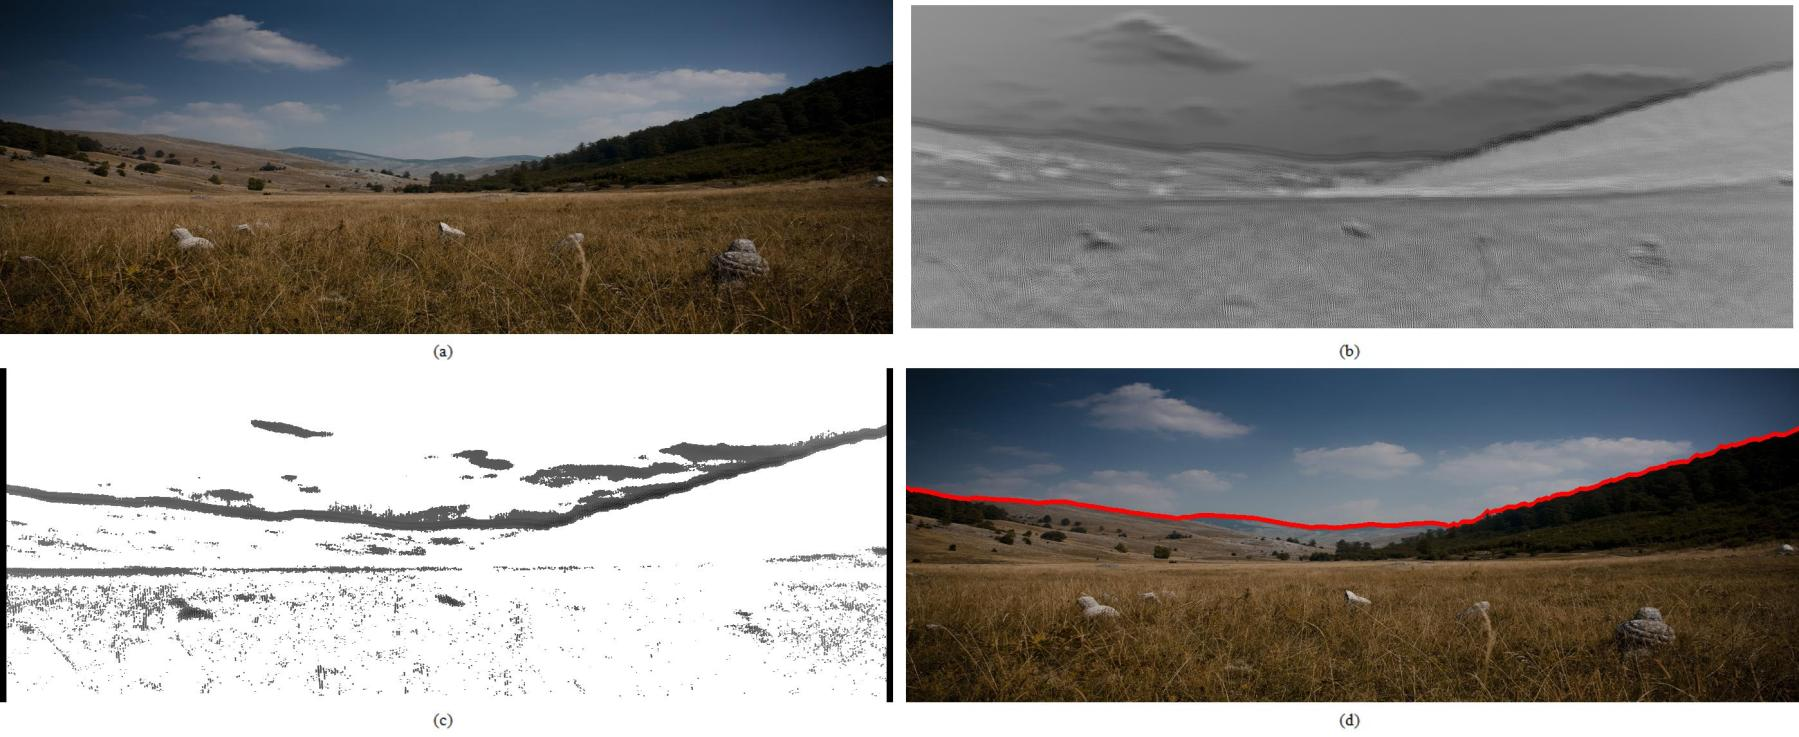
\includegraphics[width=\linewidth]{edgeless}
	\caption[Edge-less horizon detection]{\label{fig:edgeless}An edge-less horizon detection algorithm generates a dense classifier score image (DCSI) (b) from a query image (a) using trained classifiers, where a threshold is then applied (c) before it plots the horizon line (d). Reprinted with permission from~\cite{t._ahmad_edge-less_2015}}
\end{figure}

\nomenclature[z-dcsi]{DCSI}{Dense classifier score image} 

\subsection{Vanishing Point Detection} \label{secvanishing}
This is typically used in tandem or as an alternative to horizon detection to localise the vehicle with respect to the image frame. The vanishing point is a point on an image where a pair or more parallel lines in 3D space converges to. According to Rother~\cite{rother_new_2002}, the detection of a vanishing point consists of an accumulation step and a search step. The accumulation step clusters line segments that share a common vanishing point and the search step searches for dominant line clusters. Rother noted that the random sample consensus (RANSAC) method could be used to speed up vanishing point detection, to which Bazin and Pollefeys~\cite{j._c._bazin_3-line_2012}  proposed an approach that uses only three lines to achieve this. They proposed this approach for a three-degrees of freedom (3DoF) robotic manoeuvrability system similar to a ground vehicle. This effectively enables the system to estimate its rotation based on its captured visual lines and vanishing point. Kong, Audibert and Ponce~\cite{h._kong_general_2010} described an approach to road detection that centres around vanishing point detection, and their method is as illustrated in Fig.~\ref{fig:vanishingpoint}. They proposed the Locally Adaptive Self-Voting (LASV) algorithm that estimates the vanishing point based on a confidence model in a local region for texture orientation estimation. While it is more accurate than conventional voting approaches, Zhu et al.~\cite{zhu_visual_2014} noted that this approach does not perform well in suburban environments with dense roadside vegetation and fixtures. They subsequently utilised a colour histogram method to compare the captured image against an \textit{a priori} model to obtain the vanishing point. Still, line voting remains a popular method to achieve vanishing point detection and it is also used by Zhu et al. and other recent works~\cite{wu_novel_2016, alvarez_combining_2014, ricaud_general_2014, t._h._bui_local_2012, p._moghadam_fast_2012}. 

\nomenclature[z-ransac]{RANSAC}{Random sample concensus} 
\nomenclature[z-lasv]{LASV}{Locally adaptive self-voting} 
\nomenclature[z-dof]{DoF}{Degrees of freedom} 

\begin{figure}[H]
	\centering
	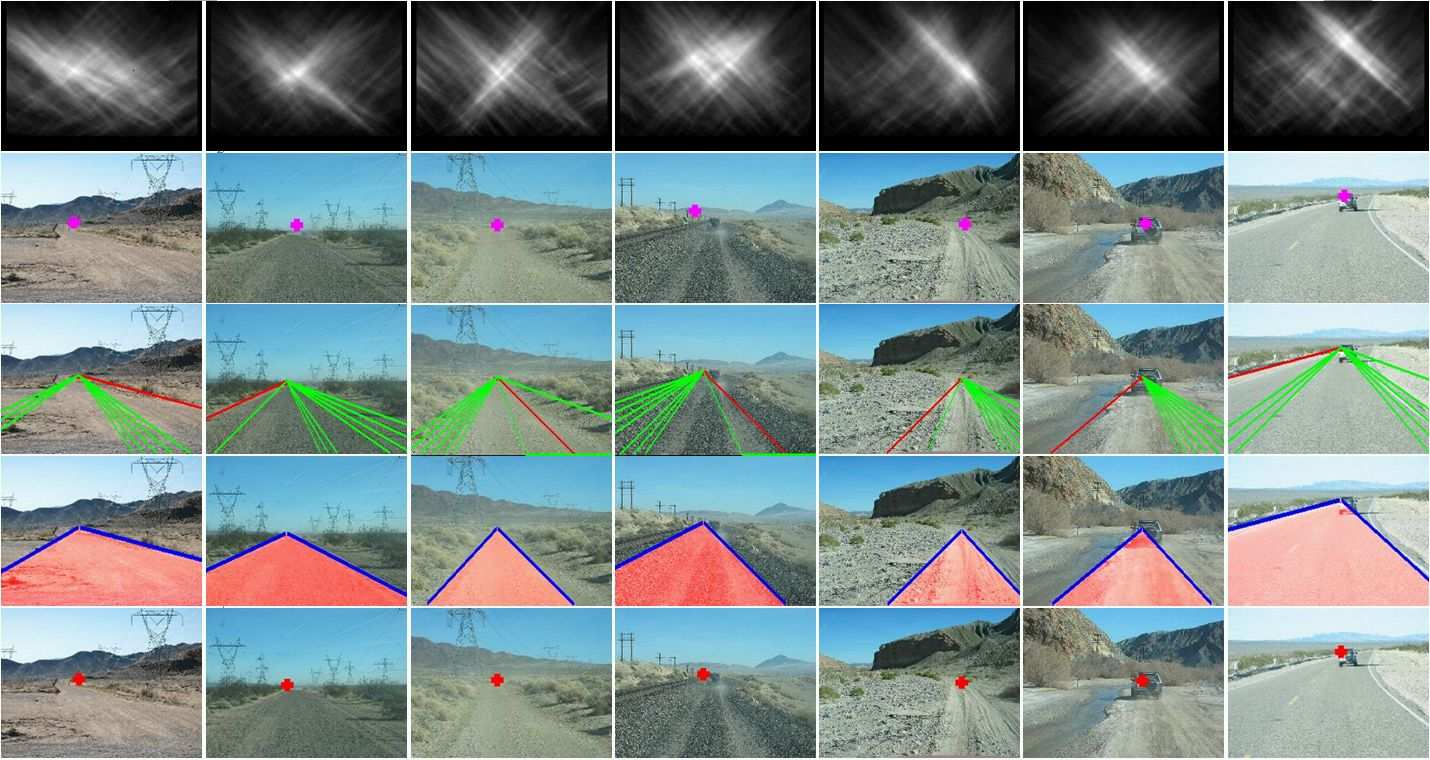
\includegraphics[width=\linewidth]{kongvanishingpoint.jpg}
	\caption[Vanishing point estimation]{\label{fig:vanishingpoint}Vanishing point estimation of seven desert road images showing the LASV algorithm. Reprinted with permission from~\cite{h._kong_general_2010}.}
\end{figure}

\subsection{Region of Interest Isolation} \label{secregion}
ROI isolation methods are used as a popular approach to recognise road segments from non-road segments. An ROI is usually identified and defined in frames before these image segments are classified. Instead of needing to process the entire frame, using an ROI isolates image processing to a frame's specific region to further reduce computing requirements. This may be used in tandem with horizon detection where certain regions below the horizon line are designated as the ROI. For road recognition, the ROI is generally a definitive region that encompasses both road and non-road regions or lane markings, as classification can then be drawn from processing that ROI. While conventional ROIs are usually fixed at a predetermined location on a frame, this assumes that the road boundary will always be on the same frame location~\cite{k._ghazali_road_2012,t._y._chen_vehicle_2015}. To circumvent this, adaptive ROI algorithms were proposed as a more robust solution that adjusts to illumination changes~\cite{bottazzi_adaptive_2014} or the location of vanishing points~\cite{d._ding_adaptive_2013}. 

\subsection{Image Classification} \label{secimage}
Image classification is used in this context to classify an image into road and non-road areas using a binary classifier~\cite{cristoforis_real-time_2016}. Roads are recognised through a combination of the road lane markings and road boundary. Lane markers are usually painted in high contrast from the road surface to be conspicuous to the drivers, and visual processing also benefits from this whereby good edge detection results can be obtained more easily. Conversely, variations in road lane appearances such as colours, lines and condition from wear and tear may pose a challenge for lane detection algorithms~\cite{j._c._mccall_video-based_2006}. Works that attempt to circumvent these variations include~\cite{fernando_real-time_2014,j._huang_robust_2013}. Some roads, especially non-gravel roads, are unstructured and have no lane markings at all. In these circumstances, lane detection algorithms will not work, and road boundary detection algorithms will be applied. On urban roads, the road boundary is perceived as the region where the asphalt meets an unpaved ground. Works that detect road boundaries may also use kerbs~\cite{f._oniga_curb_2011} or highway barriers~\cite{t._scharwachter_visual_2014}. More robust road boundary detection algorithms aim to work across different road types, including dirt roads and snow roads~\cite{h._kong_general_2010}; or variations to illumination and weather such as night driving and rain~\cite{j._dai_night-time_2014,shibata_detection_2014}. Techniques used for both road lane and boundary detection may vary, but they may also share some similarities, especially with the usage of edge detection algorithms. For instance, stereoscopic sensors can be used to perceive the tangible road boundaries in urban areas, which works as an alternative to radar or LiDAR~\cite{hu_roadside_2011}, or in conjunction for added robustness~\cite{c._fernandez_curvature-based_2015}. Non-urban roads commonly share the same plane as non-road areas, so such detection algorithm should be purely appearance-based. An example of such an algorithm was proposed by Crist\'{o}foris et al.~\cite{cristoforis_real-time_2016}, where they applied a mixture of Gaussians (MOG) model onto an image's ROI on HSV colour space that is converted from RGB. This more commonly known as the Gaussian mixture model (GMM). The GMM is a form of Bayesian classification, which performs decision making using the probability theory based on the maximum likelihood estimation (MLE). As its name suggests, a GMM a combination of several Gaussian distributions and hence the MLE is derived from the weighted sum of the Gaussians as the probability density function~\cite{paalanen_feature_2006}. In the context of road detection, GMM analyses the colour distribution of the road and estimates the colour model based its similarities with similar model groups. Gaussian models are widely used as a supervised learning approach to image classification.   Other works that incorporate a Gaussian model include~\cite{m._aly_real_2008,wang_adaptive_2015}. Alkhorshid et al.~\cite{alkhorshid_road_2016} used a histogram obtained from the calculation of frequency distribution of pixel values, and subsequently used candidate training to classify whether or not the ROI is fully, partially or not part of a road region; this is modelled after the AdaBoost classifier~\cite{yoav_freund_decision-theoretic_1997} that is employed to minimise weighted errors. Other methods of classification include using textural features~\cite{xiao_monocular_2016,s._strygulec_road_2013}, which assumes a homogeneous road texture that is compared to non-road textures. 

\nomenclature[z-mog]{MOG}{Mixture of Gaussians} 
\nomenclature[z-hsv]{HSV}{Hue, saturation, value} 
\nomenclature[z-gmm]{GMM}{Gaussian mixture model} 
\nomenclature[z-mle]{MLE}{Maximum likelihood estimation} 
\nomenclature[z-iou]{IoU}{Intersection over Union} 

\subsection{Model Fitting} \label{secmodel}
Once road and non-road regions have been classified in the image, navigational boundaries must be marked (fitted) to prevent the vehicle from veering off course. These boundaries can be marked more easily on marked roads using edge detection algorithms that benefit from the large gradient values. Edge filters such as the Sobel and Canny filters are commonly used~\cite{min_component-model_2015, c._siagian_mobile_2013, r._chen_research_2013}. Regions of the high gradient can then be plotted according to the filters' results. These plots will result in the road or lane boundary, and they can either be parametric, semi-parametric or non-parametric~\cite{bar_hillel_recent_2014}. Parametric models comprise mostly of straight lines~\cite{h._kong_general_2010}; semi-parametric models comprise of splines~\cite{wang_lane_2000} and polynomial curves~\cite{z._tao_lane_2013,m._revilloud_improved_2013}; and non-parametric models comprise of continuous arbitrary lines~\cite{cristoforis_real-time_2016}. Urban roads typically have well-defined lane markings and boundaries, hence these navigational boundaries can be marked with a parametric or semi-parametric model, effectively reducing computation complexity. Rural and unpaved roads may require the use of semi or non-polynomial models. Outliers are commonly present with fitting models, therefore it is also common to implement RANSAC for outlier rejection at this stage. Aly~\cite{m._aly_real_2008} used RANSAC to fit lines and splines in his lane detection algorithm, and it is applied after performing a simplified Hough transform for lane line counting. With the road/lane boundaries marked, the vehicle can then be guided to drive at the centre of the road/lane by finding the distance between its left and right boundaries. In addition to road boundaries, model fitting can also be applied for marking the horizon and path for navigation, such as the approach used by Crist\'{o}foris et al.~\cite{cristoforis_real-time_2016}. A popular technique of model fitting in road recognition is the Hough transform~\cite{richard_o._duda_use_1972}. The Hough transform is a shape analysis technique typically used to extract shape features from an image. Road detection and recognition works commonly apply Hough line transform on an edge-detected image to detect lane markings and road edges according to the aforementioned line models. This achieves road segmentation, splitting road sections for vehicles to recognise areas such as lanes and non-road areas. The Hough transform uses a voting procedure to fit lines. This means that each point that may correspond to a line section votes for the likelihood that a line section may be from. More votes are cast when more points lie on the same line, and lines with higher votes will be fitted~\cite{muhammad_opencv_2015}. Fig.~\ref{fig:lanedetect} illustrates an example of lane detection using Hough transform, the blue and red lines mark the left and right edge of the lane respectively, where a driving rule can be established to ensure that the vehicle does not cross these boundaries while driving. Works that employ the Hough transform or a similar voting approach to classify road and non-road regions are~\cite{h._kong_general_2010, abbas_novel_2016, zhu_visual_2014}.

\begin{figure}[H]
	\centering
	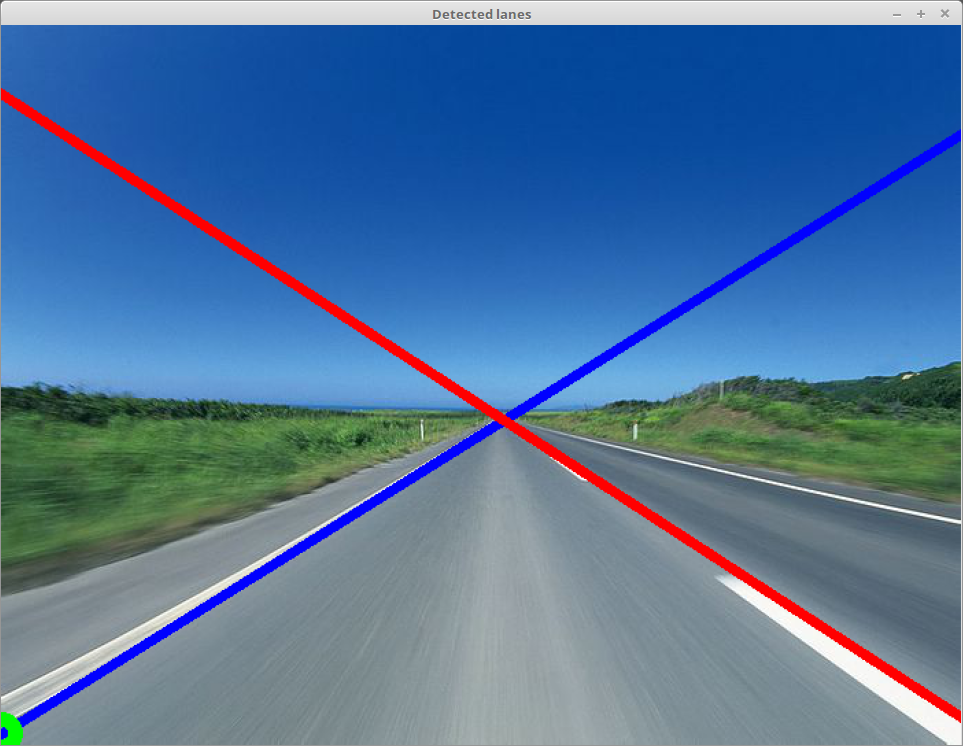
\includegraphics[width=0.5\linewidth]{lane_detection.png}
	\caption{\label{fig:lanedetect}Lane detection with Hough transform performed using OpenCV}
\end{figure}

\section{Learning Methods} \label{seclearning}
Many works are implementing learning methods these days for road recognition, where support vector machines (SVMs)~\cite{shengyan_self-supervised_2010,jian_unstructured_2009}, neural networks~\cite{m._foedisch_adaptive_2004} and AdaBoost~\cite{cord_automatic_2012} are among the more commonly implemented approaches. A neural network approach was proposed as early as 2003 by Conrad and Foedisch~\cite{p._conrad_performance_2003} using Matlab's Neural Network Toolbox. The authors compared this approach to an SVM approach and noted that while SVMs are more accurate, their computation times are long for road classification tasks. It is noted that SVM has historically been a mainstream learning method for road recognition, with newer implementations incorporating dynamic programming to account for the changes in road scenes~\cite{j._yao_estimating_2015}. Learning methods on road recognition is seeing a rise in popularity also due to the increased demand in autonomous driving, and the KITTI benchmark suite also includes are road and lane detection evaluation benchmark since 2013~\cite{jannik_fritsch_new_2013}. This benchmark categorises road scenes according to a combination of roads types including urban marked, unmarked, multiple marked lanes/roads. There are currently 336 benchmark submissions for the categories to date, using various methods such as SVM~\cite{d._a._chacra_road_2016}, CNN~\cite{oliveira_efficient_2016,mendes_exploiting_2016} and may incorporate other sensors such as LiDAR~\cite{caltagirone_fast_2017}.
%expand SVM?

\nomenclature[z-svm]{SVM}{Support vector machine} 

Due to the increased availability of parallel computers nowadays, recent works are more commonly implementing convolutional neural networks for road recognition in favour of SVM and custom networks. CNNs are feedforward neural networks with more than one convolution layer. This convolution layer applies a function repeatedly over the output of other functions, which greatly benefit from parallel computation. For road recognition, CNNs are commonly used for object detection and image segmentation, which are used on road scenes to detect and discern areas in the image that encompasses an object, where in addition to roads, it also segments other elements such as pedestrians, vehicles, vegetation and road signs. This process is commonly known as semantic segmentation. Semantic segmentation classes objects in an image according to its pixels, thereby improving the system's comprehension towards road scenes in addition to road classification over conventional learning methods, allowing for a more holistic autonomous driving system that also incorporates features such as road sign understanding, pedestrian and vehicle detection, and collision avoidance~\cite{d._kochanov_scene_2016,teichmann_multinet:_2016,badrinarayanan_segnet:_2017}. Thoma~\cite{thoma_survey_2016} and Garcia-Garcia et al.~\cite{garcia-garcia_review_2017} published surveys of semantic segmentation, which include a good background study of the underlying approaches of semantic segmentation. While the KITTI benchmark suite has not yet incorporated a semantic segmentation benchmark, it does provide a list of resources of KITTI images with semantic labels. MultiNet~\cite{teichmann_multinet:_2016} is an example that combines semantic segmentation, classification and detection for road scenes that is consolidated from the same encoder to minimise time redundancy. Results were tested and benchmarked on KITTI's road dataset where it is found to be capable of real-time processing. 

Semantic segmentation uses neural networks and is hence trained and tested on datasets. The review paper by Garcia-garcia et al.~\cite{garcia-garcia_review_2017} provides a detailed analysis of the datasets used in semantic segmentation, categorising them into 2D, 2.5D and 3D datasets. The KITTI~\cite{geiger_are_2012}, CamVid~\cite{brostow_semantic_2009} and Cityscapes~\cite{cordts_cityscapes_2016} datasets are more commonly associated with training and testing semantic segmentation for urban road scenes. The KITTI Vision Benchmark Suite is an actively maintained project by the Karlsruhe Institute of Technology and the Toyota Technological Institute of Chicago. Images were obtained by driving a car around Karlsruhe, Germany, covering a variety of road scenes. This benchmark suite spans across several categories including optical flow, stereo vision, visual odometry, and road/lane detection. The road/lane detection evaluation benchmark consists of 289 and 290 training and test images respectively. Additionally, the CamVid dataset was proposed in 2008 containing 367 training and 233 testing images. Images were obtained from the City of Cambridge, England by driving a car around. This dataset was created for semantic segmentation and each training image pixel is labelled with a different shade of grey corresponding to one of the twelve classes for road scene objects, forming the ground truth. Finally, the Cityscapes dataset was obtained from 50 cities in Germany from a road vehicle across three seasons. This is a 5000-image dataset whereby 2975, 500 and 1525 images are categorised for training, validation and testing respectively. The authors of Cityscapes made comparisons to KITTI and CamVid and noted that semantic labelling can be easily achieved with their smaller datasets and that the Cityscapes dataset provides a better challenge for new semantic segmentation approaches with its much larger dataset. Table~\ref{tabdatasets} summarises the datasets presented here according to its publication data and number of sample images for training and testing.

\begin{table}[H]
	\renewcommand{\arraystretch}{1.3}
	\caption{Summary of road datasets presented}
	\label{tabdatasets}
	\centering
	\begin{tabular}{c c c c}
		\toprule
		        \multirow{2}{*}{Dataset}         & \multirow{2}{*}{Year} & \multicolumn{2}{c}{Image Samples} \\
		             \cmidrule{3-4}              &                       & Training & Testing                \\ \midrule
		   KITTI-Road~\cite{geiger_are_2012}     & 2013                  & 289      & 290                    \\
		  CamVid~\cite{brostow_semantic_2009}    & 2009                  & 367      & 233                    \\
		Cityscapes~\cite{cordts_cityscapes_2016} & 2016                  & 2975     & 1525                   \\ \bottomrule
	\end{tabular}
\end{table}

Examples of works that focuses on semantic segmentation for road scene recognition are SegNet~\cite{badrinarayanan_segnet:_2017}, KittiSeg~\cite{teichmann_multinet:_2016} and ENet~\cite{paszke_enet:_2016}. SegNet was proposed by Badrinarayanan et al. as a CNN architecture that is often implemented on the Caffe~\cite{jia_caffe:_2014} framework. Its architecture uses an encoder-decoder network that is followed by a pixelwise classification layer, where the encoder and decoder networks consist of 13 convolutional layers each. The encoder network is the same as the VGG16~\cite{simonyan_very_2014} network, which performs convolutions to obtain a set of feature maps. The decoder network then upsamples the feature map of each corresponding encoder, producing dense feature maps that are then batch normalised. A soft-max classifier at the output then individually classifies each pixel into one of twelve object classes to form the output image as illustrated in Fig.~\ref{figsegnet}. SegNet's proposal was compared against fully convolutional network decoding technique, also based on the VGG16 network, and DeconvNet~\cite{zeiler_visualizing_2014}, which uses fully connected layers. The authors tested SegNet on the CamVid dataset and SegNet's road scene segmentation results showed that while DeconvNet and SegNet yielded favourable results, SegNet's computational cost was significantly lesser due to its network being smaller. KittiSeg is the segmentation sequence of MultiNet whereby encoding is performed using the first 13 layers of the VGG16 network like SegNet. The fully connected layers of the VGG architecture is then transformed for decoding, thereby employing a fully connected network architecture. The authors used the KITTI Road Benchmark dataset for training and noted that the network converged quickly with high road segmentation efficiencies, which placed their KittiSeg on top of KITTI's road leaderboard at the time of its publication. An example of KittiSeg's input and output on the Cityscapes dataset is as illustrated in Fig.~\ref{figkittiseg}. Paszke et al. noted that the VGG16 architecture that these works are based on are very large and hence less suitable for embedded and mobile applications, leading to the proposal of ENet~\cite{paszke_enet:_2016}. Since real-time semantic segmentation requires a frame rate of at least 10 frames per second (fps), this is difficult to achieve on embedded computers. ENet is a custom-designed neural network architecture proposed for high computational speed and accuracy that is designed based on ResNets~\cite{k._he_deep_2016}.  Performance tests showed that ENet is about 17 times faster than SegNet while running on an Nvidia Jetson TX1~\cite{nvidia_corporation_embedded_2017-1} embedded computer while being significantly more memory efficient. Training and testing benchmarks were performed across the Cityscapes, CamVid and SUN RGB-D~\cite{s._song_sun_2015} datasets with their results compared against SegNet. By measuring the intersection over union (IoU) matrices, ENet was able to outperform SegNet in the Cityscapes dataset, as well as the CamVid dataset in six of its eleven classes. Treml et al.~\cite{treml_speeding_2016} subsequently proposed a new architecture that improves on the accuracy of ENet, while being implementable on embedded computers for real-time inference. This architecture follows SegNet whereby it uses an encoder-decoder pair. The authors modified a SqueezeNet~\cite{iandola_squeezenet:_2016-1} architecture for its encoder network favouring its low latencies, and a parallel dilated convolution layer~\cite{l._c._chen_deeplab:_2017} as its decoder to retain high computation performance while using fewer parameters. Testing and training were performed on the Cityscapes dataset over the Caffe framework. Results were compared against ENet, outperforming it in its IoU matrices in both class and category, while compromising on slightly lower framerates on the Jetson TX1, but still exceeding the 10 fps requirement for autonomous driving. A summary of the semantic road segmentation algorithms are presented in Table~\ref{tabsemantic}, listing each algorithm according to its encoder-decoder network, and the datasets used for their experiments. 

\begin{figure}[H]
	\centering
	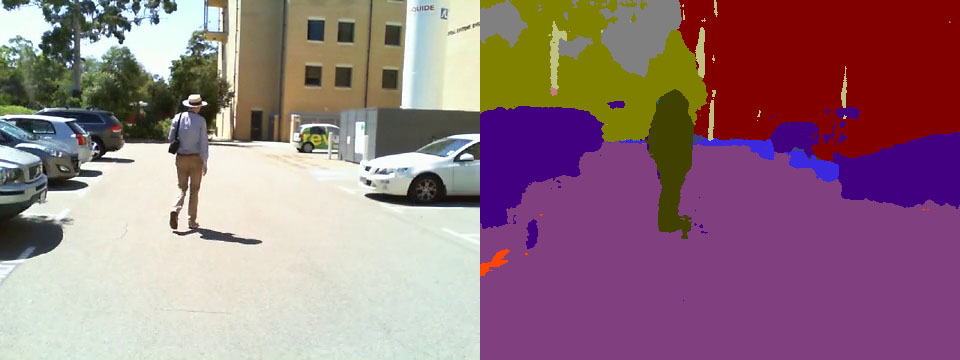
\includegraphics[width=0.8\linewidth]{segnet}
	\caption[SegNet on a Western Australian road scene]{SegNet's input (left) and output (right) for a typical Western Australian road scene.}
	\label{figsegnet}
\end{figure}

\begin{figure}[H]
	\centering
	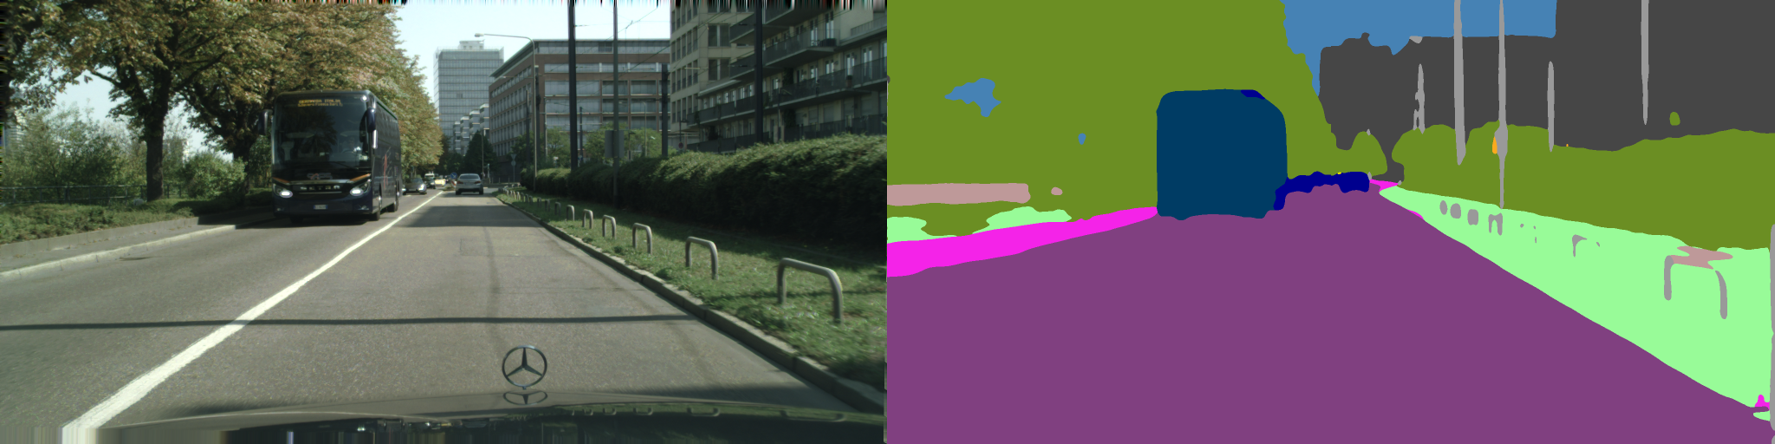
\includegraphics[width=0.8\linewidth]{kittiseg}
	\caption[KittiSeg on the Citiscapes dataset]{KittiSeg's input (left) and output (right) on the Cityscapes dataset using a Tensorflow~\cite{abadi_tensorflow:_2016} implementation. Reprinted with permission from~\cite{palazzi_github_2017}}
	\label{figkittiseg}
\end{figure}

\begin{table}[H]
	\renewcommand{\arraystretch}{1.3}
	\caption{Summary of semantic road segmentation algorithms presented}
	\label{tabsemantic}
	\centering
	\begin{tabularx}{\linewidth}{c c c >{\centering\arraybackslash}X c}
		\toprule
		           \bfseries Algorithm            & \bfseries Year & \bfseries Encoder & \bfseries Decoder             & \bfseries Dataset  \\ \midrule
		SegNet~\cite{badrinarayanan_segnet:_2017} & 2015           & VGG16             & Custom                        & CamVid             \\
		KittiSeg~\cite{teichmann_multinet:_2016}  & 2016           & VGG16             & Fully convoluted              & KITTI Road         \\
		      ENet~\cite{paszke_enet:_2016}       & 2016           & bottleneck        & bottleneck                    & CamVid, Cityscapes \\
		 Treml et al.~\cite{treml_speeding_2016}  & 2016           & SqueezeNet 1.1    & Parallel dilated convolutions & Cityscapes         \\ \bottomrule
	\end{tabularx}
\end{table}

\section{Commercial Implementations} \label{seccommercial}
Commercial implementations of road recognition in the automotive industry are largely based on the availability of original equipment manufacturers (OEMs) that supply advanced driver-assistance system (ADAS) computers and sensors. Mobileye~\cite{mobileye_mobileye_2016}, Nvidia~\cite{nvidia_corporation_nvidia_2017-1}, Velodyne~\cite{velodyne_lidar_velodyne_2017-1} and FLIR~\cite{flir_systems_flir_2017-1} are few of the OEMs involved in manufacturing autonomous driving systems. Mobileye is reputed for their ADAS system-on-chip (SoC) called EyeQ~\cite{mobileye_evolution_2017}, where in addition to lane keeping, it is capable of supporting sensor fusion, visual computing, path planning etc. towards full (Level 5~\cite{sae_international_u.s._2016-1}) autonomous driving while being power-efficient. Nvidia's DRIVE PX~\cite{nvidia_corporation_nvidia_2017-1} system uses its graphics processing unit (GPU) architectures to deliver on fast learning performance on mobile vehicles. They recently announced the Drive PX Xavier computer, which is an SoC that integrates a new GPU architecture, an eight-core central processing unit (CPU) and a computer vision accelerator with a 20 Watt requirement~\cite{shapiro_introducing_2016}, making it ideal for real-time road recognition tasks. Nvidia has also published a work describing the mapping camera pixels to steering commands using an end-to-end approach on a CNN, which is processed by the Drive PX~\cite{bojarski_end_2016}. Velodyne and FLIR are well-known OEMs that manufacture LiDAR and camera systems respectively for autonomous driving. Aside from OEMs, corporates that research into autonomous driving algorithms includes Google~\cite{waymo_waymo_2017} and Uber~\cite{etherington_ubers_2016}, as well as automotive manufacturers such as BMW~\cite{nica_bmw_2016}, Volvo~\cite{volvo_car_corporation_autonomous_2017-1} and Daimler~\cite{daimler_ag._autonomous_2017}.

\nomenclature[z-oem]{OEM}{Original equipment manufacturer} 

Road recognition and detection techniques are also becoming more accessible to the masses. As part of an effort to produce an open-sourced autonomous car, Udacity has introduced its Self-Driving Car Nanodegree Programme, which includes road and lane detection as part of its Term 1 curriculum~\cite{udacity_self-driving_2017}. Specifically, Project 1: Finding Lane Lines, and Project 4: Advanced Lane-Finding. In Project 1, students utilised OpenCV's functions such as Canny edge detection and Hough transform for road and lane detection. Project 4 expands on this to classify lane boundaries, as well as to provide the vehicle's estimated position on the road and the road's curvature. Binary images of road scenes are perspectively transformed into a bird's-eye view, where lane pixels are subsequently detected for a polynomial model fitting. The model fitted lanes can then determine the road's curvature. Fig.~\ref{figudacity} shows the final output of a Project 4 report, which includes marked lane boundaries with estimations of the lane curvatures and the vehicle's position.

\begin{figure}[H]
	\centering
	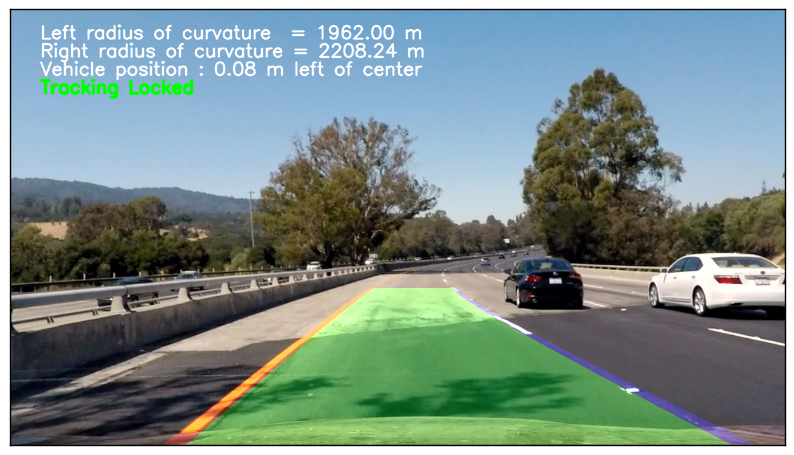
\includegraphics[width=0.7\linewidth]{udacity}
	\caption[Self-Driving Car Nanodegree output]{The Self-Driving Car Nanodegree's Term 1, Project 4 output. Reprinted with permission from~\cite{anthony_github_2017}.}
	\label{figudacity}
\end{figure}

comma.ai~\cite{comma._ai_comma.ai_2017} is a startup company by George Hotz that specialises in providing assisted and autonomous driving systems to the consumer market. Their goal is to achieve fully autonomous driving with existing road vehicles with after-market devices. Most of the software that comma.ai creates are open-sourced, which includes its autonomous driving system, openpilot~\cite{comma._ai_openpilot_2017}. openpilot performs adaptive cruise control and lane keeping that can be retrofitted to existing cars. comma.ai also includes semantic segmentation for road scenes~\cite{comma.ai_self_2016}, where they have experimented with SegNet and ENet, and proposed a solution based on ENet and ReSeg with VGG convolutional layers~\cite{visin_reseg:_2016} dubbed Suggestions Network (SugNet) to automatically label ground truths. This is in addition to the recurrent neural network approach that they took with autoencoders to learn a driving simulator as part of their initial research, which generates realistic road image predictions~\cite{santana_learning_2016}. 

\section{Recent Works} \label{secrecent}
Recent research developments in road detection are inclining towards supervised learning and neural networks. For instance, Brust et al.~\cite{brust_convolutional_2015} described an approach that uses an image patch that is fed into a CNN for label estimation, dubbed the Convolutional Patch Network. The image patch is used as the spatial prior for this method, which corresponds to a position of an object from a small group of pixels in the image frame. Among the other implementation methods proposed by the authors is a normalised initialisation approach to neural network parameters, thereby circumventing the vanishing gradient problem. For benchmarking, the authors used the KITTI dataset in a bird's-eye view. This means that a transformation was done to convert dashboard view (ego view) images into bird's-eye view, to which~\cite{jannik_fritsch_new_2013} claimed that road detection is more efficient this way. Training weights are therefore chosen according to the pixel sizes after this conversion, as the authors noted that any classification errors that happens near the horizon pixels in ego view will escalate to many more pixels in bird's-eye view. Experiments performed by the authors for road detection yields a 10\% improvement over that of Alvarez et al., which is largely contributed to the addition of spatial priors into the network. Visual road recognition implementations for autonomous driving are sometimes performed on mobile robots due to local legislation and safety concerns on autonomous vehicles~\cite{ofjall_visual_2016}. \"{O}fj\"{a}ll et al.~\cite{ofjall_visual_2016} developed a road-following system that incorporates supervised and self-reinforcement learning called symbiotic online learning of associations and regression (SOLAR). The system is initially trained by a human driver with a recording camera for the system to learn the road's appearance, whereupon sufficient training, the system will be capable of taking over controls from the driver. The system predicts visual feature vectors of subsequent frames using a Hebbian associate learning procedure~\cite{ofjall_biologically_2014}, allowing the system to perform self-feedbacks for reinforcement learning. The authors implemented SOLAR on a remote controllable robot car in environments that simulate real roads, and subsequently compared its autonomous driving capability and learning time to qHebb~\cite{ofjall_biologically_2014}, along with a CNN approach with the Caffe framework. Results showed that the CNN approach is incapable of running in real time with long learning times. Comparisons with qHebb notes that SOLAR is able to simultaneously improve learning speeds due to its reinforcement learning.  Another work that implements road detection on a mobile robot for testing is the visual road following approach by Krajn{\'i}k et al.~\cite{tomas_krajnik_visual_2015}. It shares some similarities with Crist\'{o}foris et al.'s~\cite{cristoforis_real-time_2016} work whereby it produces a path guide for the autonomous navigation of a mobile robot. This work, however, emphasises on their photometric methods that adjust to the reflectance of captured objects for shadow removal, hence providing an illumination invariant solution for visual road recognition. For testing, the authors implemented two threads in parallel; one for manoeuvring the robot, and the other calculates the robot's orientation with respect to the path boundary. This effectively ensures that the robot navigates at the centre of the path. An image captured by the robot's onboard camera is processed into an intrinsic image --- a process that decomposes an image into multiple layers of intrinsic properties. Using intrinsic images enables the algorithm to be illumination invariant. The authors subsequently used the intrinsic images to compute the robot's path through histogram equalisation, which segments the path from the background, thus binary classifying them into path and non-path regions. The robot's orientation for navigation is then calculated from a probability distribution estimation of intrinsic pixels from a histogram based on Shannon entropy~\cite{c._e._shannon_mathematical_1948}. Experiments were conducted offline using datasets and online on a mobile robot, and the results proved that using intrinsic images allows the robot to move autonomously across different illumination conditions.

\nomenclature[z-solar]{SOLAR}{Symbiotic online learning of associations and regression} 

\section{Conclusion} \label{secconclusion}
This paper presented a review of literature that covers the visual road recognition process according to its associated methods, followed by methods that incorporate machine learning, and a brief review of current commercial implementations. In a typical chronology, a methodological approach starts with horizon detection under the assumption that all road regions are below the horizon, which effectively isolates and segregates the sky portion above the horizon from any image processing. Subsequently, detecting vanishing points allows us to find the point of convergence between the road and the horizon, enabling horizon and road segmentation to be performed corresponding to that vanishing point. The road region below the vanishing point can be further segmented for computation efficiency by the introduction of the region of interests, which usually encapsulates the road or its edges where computation can be concatenated. Computational processes for visual road detection generally involves binary image classification, which classifies roads from non-road regions using techniques ranging from Gaussian models to histograms. Recently, many works incorporate CNN for visual classification with improved accuracies. With image classification complete, model fitting is applied to visually distinguish roads from non-road areas. There is also a recent shift in road recognition approaches using deep learning whereby semantic segmentation is increasingly utilised for road detection, along with other objects in road scenes. From a hardware perspective, visual road recognition is quickly replacing conventional methods such as using LiDAR and radar due to the rapid improvements in the cost and availability of image sensors. With the general availability of datasets and libraries such as KITTI and OpenCV, along with open-source deep learning libraries such as Caffe and Tensorflow, visual road recognition is now easily implementable and evaluated even in embedded systems. Additionally, recent approaches in visual road recognition are steadily addressing the research challenges presented in this area, which encompass those that are generally found in visual computing, such as illumination invariance and camera distortions. Therefore, a robust visual road recognition system should provide high accuracies while maintaining real-time computation capabilities that are able to compensate for the dynamic changes in road scenes at any time.

\section*{Acknowledgment}

The authors would like to thank Mr Andrea Palazzi, Mr Thomas Anthony, Mr Touqeer Ahmad and Prof Hui Kong for the granting of permission to use their figures in this paper.

%%*******************************************************************************
%%****************************** Second Chapter *********************************
%%*******************************************************************************
%
%\chapter{My second chapter}
%
%\ifpdf
%    \graphicspath{{Chapter2/Figs/Raster/}{Chapter2/Figs/PDF/}{Chapter2/Figs/}}
%\else
%    \graphicspath{{Chapter2/Figs/Vector/}{Chapter2/Figs/}}
%\fi
%
%
%\section[Short title]{Reasonably long section title}
%
%% Uncomment this line, when you have siunitx package loaded.
%%The SI Units for dynamic viscosity is \si{\newton\second\per\metre\squared}.
%I'm going to randomly include a picture Figure~\ref{fig:minion}.
%
%
%If you have trouble viewing this document contact Krishna at: \href{mailto:kks32@cam.ac.uk}{kks32@cam.ac.uk} or raise an issue at \url{https://github.com/kks32/phd-thesis-template/}
%
%
%\begin{figure}[htbp!] 
%\centering    
%
\includegraphics[width=1.0\textwidth]{minion}
%\caption[Minion]{This is just a long figure caption for the minion in Despicable Me from Pixar}
%\label{fig:minion}
%\end{figure}
%
%
%\section*{Enumeration}
%Lorem ipsum dolor sit amet, consectetur adipiscing elit. Sed vitae laoreet lectus. Donec lacus quam, malesuada ut erat vel, consectetur eleifend tellus. Aliquam non feugiat lacus. Interdum et malesuada fames ac ante ipsum primis in faucibus. Quisque a dolor sit amet dui malesuada malesuada id ac metus. Phasellus posuere egestas mauris, sed porta arcu vulputate ut. Donec arcu erat, ultrices et nisl ut, ultricies facilisis urna. Quisque iaculis, lorem non maximus pretium, dui eros auctor quam, sed sodales libero felis vel orci. Aliquam neque nunc, elementum id accumsan eu, varius eu enim. Aliquam blandit ante et ligula tempor pharetra. Donec molestie porttitor commodo. Integer rutrum turpis ac erat tristique cursus. Sed venenatis urna vel tempus venenatis. Nam eu rhoncus eros, et condimentum elit. Quisque risus turpis, aliquam eget euismod id, gravida in odio. Nunc elementum nibh risus, ut faucibus mauris molestie eu.
% Vivamus quis nunc nec nisl vulputate fringilla. Duis tempus libero ac justo laoreet tincidunt. Fusce sagittis gravida magna, pharetra venenatis mauris semper at. Nullam eleifend felis a elementum sagittis. In vel turpis eu metus euismod tempus eget sit amet tortor. Donec eu rhoncus libero, quis iaculis lectus. Aliquam erat volutpat. Proin id ullamcorper tortor. Fusce vestibulum a enim non volutpat. Nam ut interdum nulla. Proin lacinia felis malesuada arcu aliquet fringilla. Aliquam condimentum, tellus eget maximus porttitor, quam sem luctus massa, eu fermentum arcu diam ac massa. Praesent ut quam id leo molestie rhoncus. Praesent nec odio eget turpis bibendum eleifend non sit amet mi. Curabitur placerat finibus velit, eu ultricies risus imperdiet ut. Suspendisse lorem orci, luctus porta eros a, commodo maximus nisi.
%
%Nunc et dolor diam. Phasellus eu justo vitae diam vehicula tristique. Vestibulum vulputate cursus turpis nec commodo. Etiam elementum sit amet erat et pellentesque. In eu augue sed tortor mollis tincidunt. Mauris eros dui, sagittis vestibulum vestibulum vitae, molestie a velit. Donec non felis ut velit aliquam convallis sit amet sit amet velit. Aliquam vulputate, elit in lacinia lacinia, odio lacus consectetur quam, sit amet facilisis mi justo id magna. Curabitur aliquet pulvinar eros. Cras metus enim, tristique ut magna a, interdum egestas nibh. Aenean lorem odio, varius a sollicitudin non, cursus a odio. Vestibulum ante ipsum primis in faucibus orci luctus et ultrices posuere cubilia Curae; 
%\begin{enumerate}
%\item The first topic is dull
%\item The second topic is duller
%\begin{enumerate}
%\item The first subtopic is silly
%\item The second subtopic is stupid
%\end{enumerate}
%\item The third topic is the dullest
%\end{enumerate}
%Morbi bibendum est aliquam, hendrerit dolor ac, pretium sem. Nunc molestie, dui in euismod finibus, nunc enim viverra enim, eu mattis mi metus id libero. Cras sed accumsan justo, ut volutpat ipsum. Nam faucibus auctor molestie. Morbi sit amet eros a justo pretium aliquet. Maecenas tempor risus sit amet tincidunt tincidunt. Curabitur dapibus gravida gravida. Vivamus porta ullamcorper nisi eu molestie. Ut pretium nisl eu facilisis tempor. Nulla rutrum tincidunt justo, id placerat lacus laoreet et. Sed cursus lobortis vehicula. Donec sed tortor et est cursus pellentesque sit amet sed velit. Proin efficitur posuere felis, porta auctor nunc. Etiam non porta risus. Pellentesque lacinia eros at ante iaculis, sed aliquet ipsum volutpat. Suspendisse potenti.
%
%Ut ultrices lectus sed sagittis varius. Nulla facilisi. Nullam tortor sem, placerat nec condimentum eu, tristique eget ex. Nullam pretium tellus ut nibh accumsan elementum. Aliquam posuere gravida tellus, id imperdiet nulla rutrum imperdiet. Nulla pretium ullamcorper quam, non iaculis orci consectetur eget. Curabitur non laoreet nisl. Maecenas lacinia, lorem vel tincidunt cursus, odio lorem aliquet est, gravida auctor arcu urna id enim. Morbi accumsan bibendum ipsum, ut maximus dui placerat vitae. Nullam pretium ac tortor nec venenatis. Nunc non aliquet neque. 
%
%\section*{Itemize}
%\begin{itemize}
%\item The first topic is dull
%\item The second topic is duller
%\begin{itemize}
%\item The first subtopic is silly
%\item The second subtopic is stupid
%\end{itemize}
%\item The third topic is the dullest
%\end{itemize}
%
%\section*{Description}
%\begin{description}
%\item[The first topic] is dull
%\item[The second topic] is duller
%\begin{description}
%\item[The first subtopic] is silly
%\item[The second subtopic] is stupid
%\end{description}
%\item[The third topic] is the dullest
%\end{description}
%
%
%\clearpage
%
%\tochide\section{Hidden section}
%\textbf{Lorem ipsum dolor sit amet}, \textit{consectetur adipiscing elit}. In magna nisi, aliquam id blandit id, congue ac est. Fusce porta consequat leo. Proin feugiat at felis vel consectetur. Ut tempus ipsum sit amet congue posuere. Nulla varius rutrum quam. Donec sed purus luctus, faucibus velit id, ultrices sapien. Cras diam purus, tincidunt eget tristique ut, egestas quis nulla. Curabitur vel iaculis lectus. Nunc nulla urna, ultrices et eleifend in, accumsan ut erat. In ut ante leo. Aenean a lacinia nisl, sit amet ullamcorper dolor. Maecenas blandit, tortor ut scelerisque congue, velit diam volutpat metus, sed vestibulum eros justo ut nulla. Etiam nec ipsum non enim luctus porta in in massa. Cras arcu urna, malesuada ut tellus ut, pellentesque mollis risus.Morbi vel tortor imperdiet arcu auctor mattis sit amet eu nisi. Nulla gravida urna vel nisl egestas varius. Aliquam posuere ante quis malesuada dignissim. Mauris ultrices tristique eros, a dignissim nisl iaculis nec. Praesent dapibus tincidunt mauris nec tempor. Curabitur et consequat nisi. Quisque viverra egestas risus, ut sodales enim blandit at. Mauris quis odio nulla. Cras euismod turpis magna, in facilisis diam congue non. Mauris faucibus nisl a orci dictum, et tempus mi cursus.
%
%Etiam elementum tristique lacus, sit amet eleifend nibh eleifend sed \footnote{My footnote goes blah blah blah! \dots}. Maecenas dapibu augue ut urna malesuada, non tempor nibh mollis. Donec sed sem sollicitudin, convallis velit aliquam, tincidunt diam. In eu venenatis lorem. Aliquam non augue porttitor tellus faucibus porta et nec ante. Proin sodales, libero vitae commodo sodales, dolor nisi cursus magna, non tincidunt ipsum nibh eget purus. Nam rutrum tincidunt arcu, tincidunt vulputate mi sagittis id. Proin et nisi nec orci tincidunt auctor et porta elit. Praesent eu dolor ac magna cursus euismod. Integer non dictum nunc.
%
%
%\begin{landscape}
%
%\section*{Subplots}
%I can cite Wall-E (see Fig.~\ref{fig:WallE}) and Minions in despicable me (Fig.~\ref{fig:Minnion}) or I can cite the whole figure as Fig.~\ref{fig:animations}
%
%
%\begin{figure}
%  \centering
%  \begin{subfigure}[b]{0.3\textwidth}
%    
\includegraphics[width=\textwidth]{TomandJerry}
%    \caption{Tom and Jerry}
%    \label{fig:TomJerry}   
%  \end{subfigure}             
%  \begin{subfigure}[b]{0.3\textwidth}
%    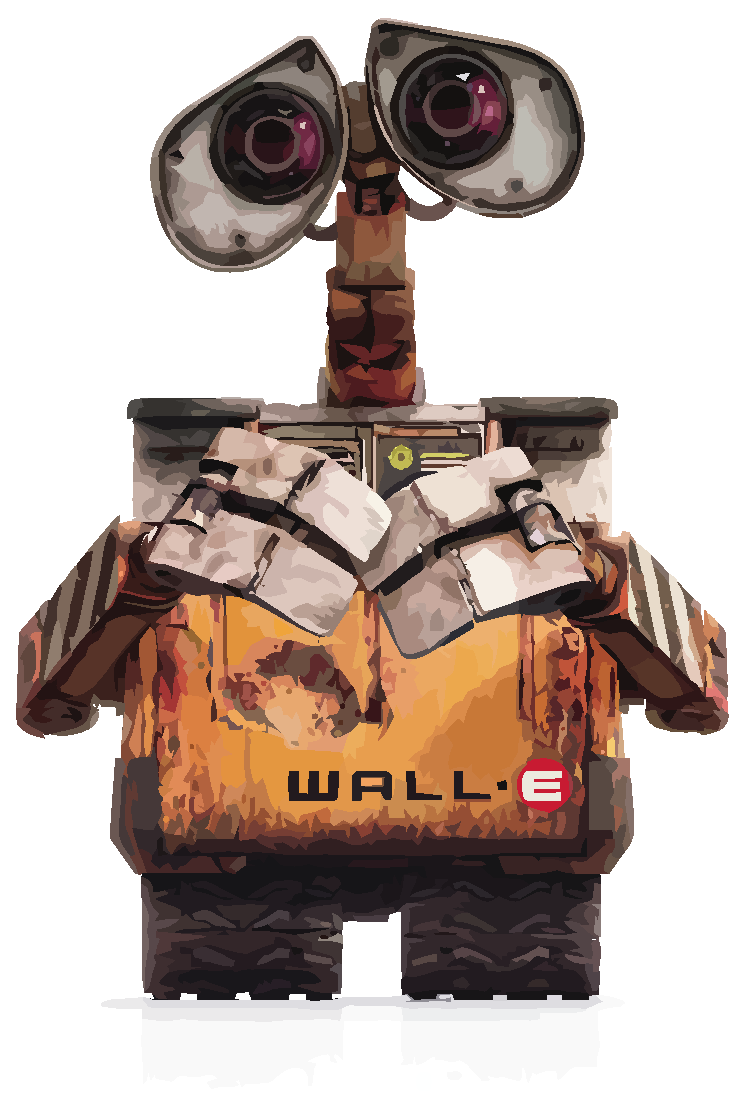
\includegraphics[width=\textwidth]{WallE}
%    \caption{Wall-E}
%    \label{fig:WallE}
%  \end{subfigure}             
%  \begin{subfigure}[b]{0.3\textwidth}
%    
\includegraphics[width=\textwidth]{minion}
%    \caption{Minions}
%    \label{fig:Minnion}
%  \end{subfigure}
%  \caption{Best Animations}
%  \label{fig:animations}
%\end{figure}
%
%
%\end{landscape}

%!TEX root = ../thesis.tex

\chapter[Visual Odometry Review]{A Review of Visual Odometry Methods and Its Applications for Autonomous Driving}
\label{ch:voreview}

\ifpdf
\graphicspath{{Chapter3/Figs/Raster/}{Chapter3/Figs/PDF/}{Chapter3/Figs/}}
\else
\graphicspath{{Chapter3/Figs/Vector/}{Chapter3/Figs/}}
\fi

The research into autonomous driving applications has observed an increase in computer vision-based approaches in recent years. In attempts to develop exclusive vision-based systems, visual odometry is often considered as a key element to achieve motion estimation and self-localisation, in place of wheel odometry or inertial measurements. This paper presents a recent review to methods that are pertinent to visual odometry with an emphasis on autonomous driving. This review covers visual odometry in their monocular, stereoscopic and visual-inertial form, individually presenting them with analyses related to their applications. Discussions are drawn to outline the problems faced in the current state of research, and to summarise the works reviewed. This paper concludes with future work suggestions to aid prospective developments in visual odometry.

\section{Introduction}
Autonomous driving has come a long way since it was first promoted in the DARPA Urban Challenge back in 2007~\cite{buehler_darpa_2009}. With major car manufacturers lobbying their technologies in autonomous driving, the ownership of autonomous vehicles is set to rise in the future. Current autonomous vehicles rely on a variety of sensors to achieve self-localisation and obstacle avoidance. These can include a combination of laser scanners, radar, GPS, and camera. However, the installation of sensor arrays on a vehicle greatly increases its cost and complexity. At the same time, the increasing affordability and ubiquity of cameras and high-performance graphics processing units (GPUs) are catalysing the resurgence of image processing and computer vision applications. In other words, these applications that were once computationally expensive, are gradually replacing tasks that were performed using other sensors and methods. These tasks include the motion estimation of the vehicle, where precise odometry is crucial for the accurate localisation of the autonomous vehicle. The odometry problem exists such that conventional GPS sensors are unable to provide the necessary road lane precision ($\approx3$ m), and that it is unable to function indoors such as inside tunnels and buildings. Additionally, standard wheel odometry suffers from accumulating drift errors that increase over time. While the use of sensors such as high precision differential GPS and inertial sensors could alleviate this problem, they are significantly more expensive to purchase than a standard camera setup. 

Visual odometry (VO) is a research area that is becoming increasingly popular in recent years. Ground vehicles and robots rely on odometry to measure and record their traversed path as they navigate, making this an essential component for autonomous navigation. Visual odometry is odometry that is performed by analysing visual data such as one from a mounted camera. This concept was first proposed by Moravec in~\cite{hans_peter_moravec_obstacle_1980}, and the term ``visual odometry'' was coined by Nistér et al. in~\cite{nister_visual_2006}. Conventional wheel odometry estimates a robot's position by measuring the wheel rotation using sensors from the servos. A common issue experienced by wheel odometry is wheel slip, whereby pose estimations becomes incrementally inaccurate from the occasional loss of traction from the wheels. Visual odometry negates this problem.

\nomenclature[z-vo]{VO}{Visual odometry}
VO techniques can be classified according to their utilised imagery --- either stereoscopic or monocular visual odometry, and their processing techniques --- either feature-based or direct (image/appearance-based). These methods can either use a combination of feature matching, feature tracking or optical flow ~\cite{scaramuzza_visual_2011, yousif_overview_2015}. Since a majority of visual odometry implementation recreates a 3D navigation environment from a set of captured images, most approaches are of a stereoscopic approach that utilises a pair of mounted cameras on the robot. By accounting for the cameras' capture frame rate and the distance between them, the robot's displacement and velocity from an object can be calculated with ease through the triangulation of image features~\cite{hartley_triangulation_1997}. Therefore, the monocular visual odometry problem is more complex and it is not until recently that we are starting to see an increasing trend in this area. Monocular visual odometry achieves motion estimation and environment recreation through a combination of a series of at least three 2D images in series, along with its bearing data. An adaptation of the parallel tracking and mapping (PTAM) algorithm~\cite{georg_klein_parallel_2007} is used in many monocular implementations. PTAM is originally devised for augmented reality (AR) implementations, but its speed and robustness while relying only on existing map features made it a popular choice for researchers of visual odometry. 

\nomenclature[z-ptam]{PTAM}{Parallel tracking and mapping}

On the processing techniques front, feature-based approaches achieve motion estimation by extracting image features such as lines and edges, and tracking them in subsequent frames; by calculating the Euclidean distances of each feature points between frames, the displacement and velocity vectors can be calculated. Direct approaches use pixels in an image frame and track the changes in pixel intensity~\cite{valiente_garcia_visual_2012}, where pixel selection can either be all pixels (dense) or sparsely selected (sparse). In feature-based approaches, feature matching detects and tags existing features on a given set of frames. Feature extraction and matching techniques such as Scale Invariant Feature Transform (SIFT)~\cite{lowe_distinctive_2004}, Features From Accelerated Segment Test (FAST)~\cite{rosten_machine_2006}, Speeded Up Robust Features (SURF)~\cite{bay_speeded-up_2008}, Binary Robust Independent Elementary Features (BRIEF)~\cite{calonder_brief:_2010} and Oriented FAST and Rotated BRIEF (ORB)~\cite{e._rublee_orb:_2011} are some of the more commonly implemented ones in literature. Feature tracking techniques allow features to be tracked across subsequent frames. This is usually used in tandem with features obtained from a feature extraction technique. Feature tracking is essential for visual odometry, as it allows the robot to achieve a consistent measurement to localise itself~\cite{yousif_overview_2015}. Varying conditions in the environment such as lighting conditions and dynamic obstacles can impede accuracy with outliers. To circumvent this, many works employ the Random Sampling Consensus (RANSAC)~\cite{martin_a._fischler_random_1981} outlier rejection scheme or a variation of it; more recently, Buczko and Willert have also proposed an outlier detection scheme for monocular~\cite{buczko_monocular_2017} and stereoscopic~\cite{buczko_how_2016} approaches. Finally, optical flow allows the robot to estimate its distance from an environmental object by tracking its features from the robot's camera feed. With optical flow, the robot can perform obstacle detection and avoidance during navigation. An optical flow algorithm outputs an image pattern that relates to the movement of objects within the robot's field of view (FOV). Examples of popular optical flow algorithms include the Lucas and Kanade's~\cite{bruce_iterative_1981}, Horn and Schunck's~\cite{horn_determining_1981}, Farneback's~\cite{farneback_two-frame_2003}, and SimpleFlow~\cite{tao_simpleflow:_2012} algorithms. Optical flow algorithms can either be dense (tracks a full frame) or sparse (tracks extracted features). Dense optical flow requires greater computation performance, whereas sparse optical flow methods employ feature extraction prior to its computation to make it less intensive. 

\nomenclature[z-fast]{FAST}{Features from accelerated segment test}
\nomenclature[z-brief]{BRIEF}{Binary Robust Independent Elementary Features}
\nomenclature[z-orb]{ORB}{Oriented FAST and rotated BRIEF}
\nomenclature[z-fov]{FOV}{Field of view}

It is also common for researchers to use a combination of the three processing techniques to achieve robust optical flow. For example, Wang and Schmid~\cite{wang_action_2013} used a combination of SURF descriptors, RANSAC for outlier rejection, and dense optical flow to achieve the prediction of human actions. Liu et al.~\cite{liu_maximum_2016} proposed an optical flow approach based on the Maximum Likelihood Estimation (MLE), which is implemented on a mobile robot and compared against their RANSAC development for optical flow; they concluded that their MLE approach is more accurate than the RANSAC approach. More recently, Kroeger et al.~\cite{kroeger_fast_2016} proposed a faster approach for dense optical flow computation using the dense inverse search (DIS)~\cite {s._baker_equivalence_2001} method, noting that many optical flow proposals have neglected time complexity in favour of accuracy. The authors' evaluation of the DIS fast optical flow showed that while it introduced slight estimation errors, it is much faster even when compared to newer optical flow methods. 

\nomenclature[z-dis]{DIS}{Dense inverse search}

This paper reviews monocular and stereoscopic VO methods according to their procedures to achieve motion estimation, as well as their methods of evaluation. A shorter section on visual-inertial odometry is also presented to explore works that combine inertial measurements for VO. The review of these VO methods intends to gauge their suitability for use in real-time, on-line autonomous driving, which is motivated by the research gap in VO applications for autonomous vehicles. The aim of this article is hence to understand the current trends in VO and to determine if the current state of VO is adequate enough to be utilised in autonomous vehicles. 

This paper reviews monocular and stereoscopic VO methods according to their procedures to achieve motion estimation, as well as their methods of evaluation. A shorter section on visual-inertial odometry is also presented to explore works that combine inertial measurements for VO. The review of these VO methods intends to gauge their suitability for use in real-time, on-line autonomous driving, which is motivated by the research gap in VO applications for autonomous vehicles. The aim of this article is hence to understand the current trends in VO and to determine if the current state of VO is adequate enough to be utilised in autonomous vehicles. 

\begin{figure}[ht]
	\centering
	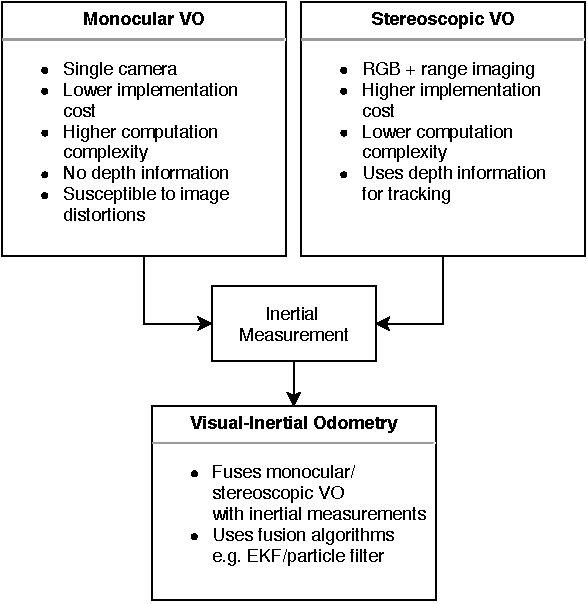
\includegraphics[width=0.5\linewidth]{VO-Imagery.pdf}
	\caption[Types of VO approaches]{Types of VO approaches as classified by their imagery methods. Visual-inertial odometry is VO that is fused with inertial measurements.}
	\label{fig:3:imagery}
\end{figure}

\begin{figure}[ht]
	\centering
	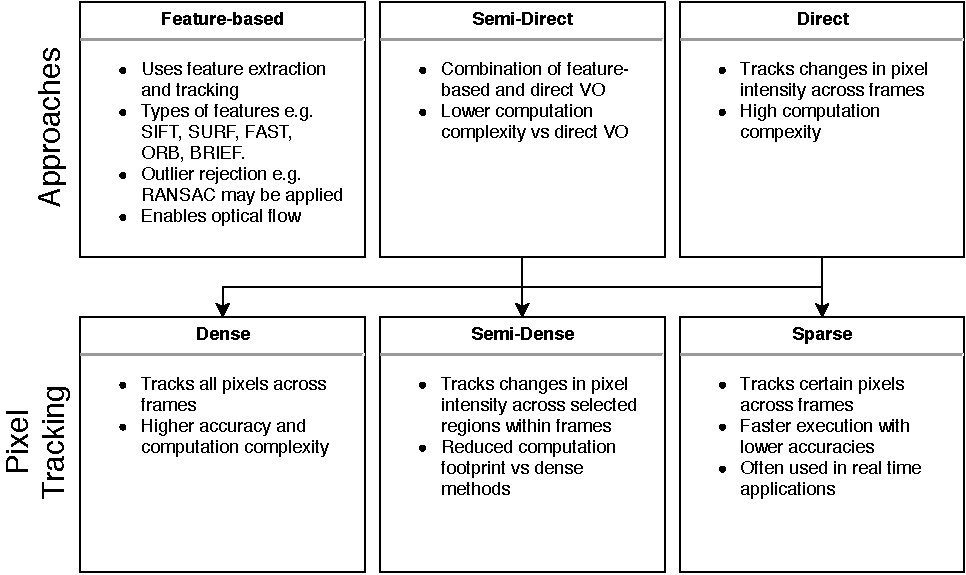
\includegraphics[width=0.9\linewidth]{VO-Processing.pdf}
	\caption[VO processing techniques]{Processing techniques used in VO according to their approaches and their pixel tracking methods for direct approaches.}
	\label{fig:3:processing}
\end{figure}

Figures~\ref{fig:3:imagery} and ~\ref{fig:3:processing} summarise the scope of this paper. The remainder of this paper is organised according to imagery techniques given in  Figure~\ref{fig:3:imagery}, whereby Sections~\ref{sec:3:mvo} through~\ref{sec:3:vio} describes monocular VO, stereoscopic VO and visual-inertial odometry respectively; Section~\ref{sec:3:discuss} presents critical discussions from our review findings in relation to autonomous driving before the conclusion is drawn in Section~\ref{sec:3:concl}. Reviews will emphasise on the VO approaches and for direct methods, the pixel tracking density according to Figure~\ref{fig:3:processing}, which is further elaborated in Section~\ref{sec:3:mvo}.

\section{Monocular Visual Odometry}\label{sec:3:mvo}
Using a monocular camera setup for VO benefit implementations that are lower in cost and complexity. A monocular setup will also alleviate the decrease in depth measurement accuracies as the distance between the camera and the scene increases beyond the stereo baseline. This setup, however, introduces several challenges in addition to the lack of depth measurements on a stereoscopic setup. This was pointed out by Yang et al.~\cite{yang_challenges_2017}, where they have investigated several challenges that pertain to this area namely photometric calibration, motion bias, and (assuming that a roller shutter camera is used) the rolling shutter effect. Photometric calibration is required as the pixel intensity for a same 3D point will experience varying values due to the changes in camera adjustment such as optical exposures and gains; motion bias notes that VO performances are different for forward and backward playback on the same sequence; and the rolling shutter effect is predominantly present in rolling shutter cameras whereby an image will distort in while a camera is in motion as the frame is captured line by line. The authors then analysed these challenges using a feature-based method, a semi-direct method, and a direct method, which are ORB-SLAM~\cite{mur-artal_orb-slam2:_2017}, SVO~\cite{forster_svo:_2017} and DSO~\cite{engel_direct_2018} respectively. The several conclusions drawn from this analysis allowed us to deduce that direct methods are more robust with photometric calibration while being insensitive to pixel discretisation artefacts; while it is affected by the rolling shutter effect, in terms of autonomous driving, using a global shutter camera will nullify this. 

\nomenclature[z-svo]{SVO}{Semidirect visual odometry}
\nomenclature[z-dso]{DSO}{Direct sparse odometry}
\nomenclature[z-slam]{SLAM}{Simultaneous localisation and mapping}

For feature-based VO, Chien et al.~\cite{chien_when_2016} compared the SIFT, SURF, ORB and A-KAZE~\cite{alcantarilla_fast_2013} feature extraction methods for monocular VO. Experiments were conducted on the KITTI dataset using OpenCV 3.1, and concluded that while SIFT is the most accurate at extracting features, ORB is less computationally intensive, the A-KAZE method sits between SIFT and ORB in computational requirements and accuracy. We hence decided that as our autonomous driving implementation uses an embedded computer, the ORB method is better suited for our applications. 

Prominent monocular VO algorithms that are recently proposed include Direct Sparse Odometry (DSO)~\cite{engel_direct_2018} and Semidirect Visual Odometry (SVO)~\cite{forster_svo:_2017}. As their names suggest, DSO uses a direct approach whereas SVO uses a semi-direct approach to monocular VO. DSO also uses a sparse formulation thereby decreasing computation complexity, as opposed to dense~\cite{newcombe_dtam:_2011, meilland_real-time_2011} and semi-dense~\cite{daftry_semi-dense_2015, engel_lsd-slam:_2014} formulations of past proposals. This meant that DSO is capable of achieving real-time computation, as it samples only points of sufficient intensity gradient, and neglecting the geometric prior. DSO functions by continuously optimising photometric parameters from the camera to achieve photometric calibration. This optimisation was performed using a Gauss-Newton method through a sliding window. DSO uses sparse technique whereby it samples data points that are of a limited and equally distributed number across space and active frames, thereby reducing sampling redundancy for data point management. Experimental results showed that DSO as a direct approach is robust against photometric noise, and is able to achieve high accuracies with proper calibration. 

SVO was proposed to solve the slow computations and lack of optimality and consistencies of direct methods by combining traits of direct and feature-based methods. This algorithm performs a minimisation of photometric errors on features of the same 3D point, where subpixel features are subsequently obtained through the relaxation of geometric constraints. The minimisation of photometric error is performed at the sparse image alignment stage using a method of least squares, where it assumes that depth information is only known at corners and features that lie on intensity edges. A sparse method uses little depth information and hence the authors enhanced its robustness by aggregating the photometric cost for pixels surrounding the feature, with approximations similar to the feature depth. SVO employs drift minimisation by relaxing geometric constraints and aligning corresponding feature patches to an older reference patch, which is subsequently optimised for reprojection errors using a bundle adjustment. To improve computation efficiency, SVO uses a second thread for mapping, which initialises a new depth filter at FAST corners at every keyframe, thereby estimating the pixel depth using a recursive Bayesian depth filter. Experiments comparing SVO against ORB-SLAM and LSD-SLAM showed that SVO is more efficient at tracking features due to its sparse approach while being robust to high-speed camera captures without the need for outlier rejection methods such as RANSAC. For application requiring high accuracies, the authors used iSAM2~\cite{kaess_isam2:_2012}, which applies incremental smoothing for the trajectory motion, thereby achieving the same accuracy as a batch estimation of the entire trajectory in real-time. SVO can also be fused with inertial measurement to further increase odometric accuracies. 

\subsection{Related Applications}
Monocular VO algorithms are often tested as a benchmark on datasets such as MonoVO~\cite{engel_photometrically_2016} and KITTI's monocular VO dataset~\cite{geiger_are_2012}. Recent works that implement monocular VO include the work by Sappa et al.~\cite{sappa_monocular_2016}, which uses fused images to achieve monocular VO through a discrete wave transform (DWT) scheme where the characteristics of the captured image determine the DWT parameters. Using an image fusion technique condenses information from multiple image frames into one before it is used for motion estimation. This method is compared against VISO2~\cite{kitt_visual_2010}, and experiments were performed on video sequences captured on vehicles driving at different times of day and location. By comparing this fusion approach with previous approaches, the authors noted that the algorithm performs well in challenging environments such as low light drives. Results during daytime are similar across all compared approaches.  

\nomenclature[z-dwt]{DWT}{Discrete wave transform}

The online supervised approach presented by Lee et al.~\cite{lee_online_2015} uses ground classification to achieve monocular VO. The authors employed an appearance-based approach with RANSAC over three successive frames to obtain the image flow. Online self-learning is achieved by combining geometric estimates with the ground classifier, which uses a histogram of colour labels. The authors tested their approach on the KITTI odometry dataset where it is compared against the VISO2 algorithm and concluded that their approach was superior in terms of stability and translation performance. While the exclusive use of ground information is adequate to achieve VO for autonomous driving, the authors noted that it could be worthwhile to extend the work to estimate other object models. 

Additionally, works that combine semantic segmentation and monocular VO include~\cite{ros_vision-based_2015, an_semantic_2017}. An et al.~\cite{an_semantic_2017} introduced a semantic-segmentation aided VO in order to identify and compensate for dynamic visual obstructions in a camera frame. A modified version of SegNet~\cite{badrinarayanan_segnet:_2017} is used to find visual cues that represent regions of actual motion. The VO method is a semi-direct method whereby in the feature-based section, the authors employed a $k$-nearest neighbour method to match keypoints from prior frames with its transformation solved using a least-square minimisation method; in the direct (alignment-based) method, the authors used a semi-dense method whereby the framework only utilises regions with certain segmentation labels to ensure that planar objects that are not in motion are selected, which are road and pavement regions, and road markings. Tests were performed on the KITTI odometry dataset and the authors' Beijing Wuhan dataset. The VO approach was compared against the VISO~\cite{geiger_stereoscan:_2011}, DSO and ORB-SLAM2 algorithms, and concluded that a semantic segmentation approach is able to compensate moving objects on the road, where the VISO, DSO and ORB-SLAM2 could not. 

The approach by~\cite{an_semantic_2017} ties into our requirements for our autonomous driving platform, as we also employ semantic segmentation to achieve visual autonomous driving. Also, the authors noted that ORB-SLAM2 achieved the best accuracy on the KITTI dataset on low traffic segments. This could also indicate that an ORB-SLAM-based method with semantic segmentation could be implemented for autonomous driving if it's properly optimised. If performance cost is an issue, we hypothesise that using a ground-only approach such as~\cite{lee_online_2015} could achieve adequate VO for autonomous driving, while neglecting dynamic road objects. A robust day-night implementation could benefit from the implementation of a fusion technique as in~\cite{sappa_monocular_2016}, but its overhead performance cost needs to be taken into consideration. A summary of the monocular VO algorithms reviewed is given in Table~\ref{tablemono}, which lists its approach type, descriptors/features, outlier rejection scheme, dataset evaluated, and intended environment.

 \begin{sidewaystable}
 	\caption{Summary of monocular VO methods reviewed}\label{tablemono}
 	\centering
 	\footnotesize
 	\begin{tabularx}{\textwidth}{X c c c c c}
 		\toprule
 		\bfseries Method & \bfseries Approach & \bfseries Descriptor & \bfseries Outlier Rejection & \bfseries Dataset & \bfseries Environment \\
 		\midrule
 		DSO~\cite{engel_direct_2018} & Direct & Photometric & Threshold filter & monoVO, EuRoC, ICL-NUIM & Aerial drone \\
 		SVO~\cite{forster_svo:_2017} & Semi-direct & Photometric + FAST & Depth filter & TUM RGB-D, EuRoC, ICL-NUIM, Circle~\cite{forster_svo:_2017} & Aerial drone \\
 		Sappa et al.~\cite{sappa_monocular_2016} & Feature & SURF (VISO2) + DWT & RANSAC & KAIST~\cite{choi_kaist_2018}, CVC~\cite{poujol_visible-thermal_2016} & Road vehicle \\
 		Lee et al.~\cite{lee_online_2015} & Direct & Geometric estimate & RANSAC & KITTI & Road vehicle \\
 		An et al.~\cite{an_semantic_2017} & Semi-direct & Photometric + SegNet & RANSAC & KITTI, Beijing Wuhan~\cite{an_semantic_2017} & Road vehicle\\
 		\bottomrule
 	\end{tabularx}

 	\caption{Summary of stereoscopic VO works reviewed}\label{tablestereo}
 	\centering
 	\footnotesize
 	\begin{tabularx}{\textwidth}{X c c c c c}
 		\toprule
 		\bfseries Method & \bfseries Approach & \bfseries Descriptor & \bfseries Outlier Rejection & \bfseries Dataset & \bfseries Environment \\
 		\midrule
 		CV4X~\cite{persson_robust_2015} & Feature & FAST + BRIEF & RANSAC & KITTI & Road vehicles\\
 		Stereo DSO~\cite{wang_stereo_2017} & Direct & Photometric & Threshold filter & KITTI, Cityscapes & Road vehicles \\
 		Wu et al.~\cite{wu_framework_2017} & Feature & KLT & RANSAC & KITTI & Road vehicles\\
 		Proen\c{c}a and Gao~\cite{proenca_probabilistic_2018} & Feature & SURF + LSD & Circle matching & TUM RGB-D, ICL-NUIM & Pedestrian (Indoor)\\
 		Holzmann, Fraundorfer and Bischof~\cite{holzmann_detailed_2016} & Direct & SAD & Cauchy Loss function & Rawseeds~\cite{ceriani_rawseeds_2009}, KITTI,~\cite{holzmann_detailed_2016} & Aerial, ground robots\\
 		Jaimez et al.~\cite{jaimez_fast_2017} & Direct & Photometric + Background Seg & \textit{None} & TUM RGB-D & N/A\\
 		Liu et al.~\cite{liu_robust_2017} & Feature & SURF (VISO2) & Circle matching & KITTI, New Tsukuba & Road vehicles\\
 		Kunii, Kovacs and Hoshi~\cite{kunii_mobile_2017} & Feature & FREAK, CenSurE & RANSAC & Real world (Izu Oshima) & Mobile robot\\
 		Sun et al.~\cite{sun_sequentially_2017} & Feature & U-SURF & RANSAC & Real world & Mobile robot \\
 		Kim and Kim~\cite{kim_effective_2016} & Direct & Photometric & t-distribution & TUM RGB-D, real world & Mobile robot \\
 		\bottomrule
 	\end{tabularx}
 \end{sidewaystable}

\section{Stereoscopic Visual Odometry}\label{sec:3:svo}
Visual odometry is stereoscopic when a depth measurement is obtainable from a range imaging/RGB-D camera, often through a stereoscopic camera which uses stereo triangulation to measure depth. Other range imaging cameras that are used for stereoscopic VO include structured-light cameras~\cite{liu_improved_2017,huang_visual_2017} and time-of-flight cameras~\cite{stefan_threedimensional_2009}. This depth measurement enables the distance between the vehicle and its surrounding objects to be perceived, thereby simplifying VO calculations. It is also possible to rely solely on this depth measurement to perform VO, as opposed to using an image-based (feature or appearance-based) approach; this is known as a depth-based approach~\cite{fang_experimental_2015}. Applications for stereoscopic VO are popular, having a list that includes the Mars rover~\cite{maimone_two_2007} and autonomous aerial drones~\cite{strydom_visual_2014}. Its popularity today can be attributed to the leaderboard on the KITTI VO benchmark~\cite{geiger_are_2012}, whereby a great proportion of the most accurate methods are stereoscopic. As opposed to a monocular approach, stereo VO requires proper calibration and synchronisation of the camera pair, as errors will directly affect VO performance~\cite{kitt_visual_2010}

\nomenclature[z-rgb]{RGB}{Red, green and blue}
\nomenclature[z-rbgd]{RGB-D}{Red, green, blue and depth}

Stereoscopic VO can also be classified from a combination of feature- or appearance-based approaches. A review was presented by Fang and Zhang~\cite{fang_experimental_2015} in 2014, which compares several stereoscopic VO methods according to their approaches. The authors tested these methods empirically on the TUM RGB-D dataset~\cite{sturm_benchmark_2012}, along with the authors' dataset collected from an indoor environment. This dataset tests the algorithms in a variety of environments with a combination of fast motion, illumination invariances and limited features. Stereo VO algorithms were measured for their accuracies and computational performances. Results showed that depth-based algorithms such as Rangeflow~\cite{jaimez_fast_2015} is robust in environments that lack features or illumination; an image-based algorithm is suitable for feature-rich environments with adequate illumination. 

It should be noted that the implementation simplicity of stereo VO, when compared to the added computation complexity of monocular VO, could imply that the research advancements made by monocular VO are more substantial than that of its stereo counterpart; this argument was pointed out by Persson et al.~\cite{persson_robust_2015}, to which they have presented a stereo VO algorithm dubbed the CV4X that leverages on monocular VO techniques. The authors selected a feature-based method using FAST descriptors for corner extraction that is filtered with an Adaptive Non-Maxima Suppression (ANMS) filter, and tracking is performed on BRIEF descriptors. The camera's pose estimation was performed using RANSAC for the perspective-$n$-point (PNP) problem. Stereo triangulation errors are minimised through an iterative minimising function. CV4X was tested on the KITTI VO dataset and subsequently achieving first place on the benchmark leaderboard at its time of publication. The performance of this algorithm was optimised using OpenMP~\cite{openmp_openmp_nodate} and CUDA~\cite{nvidia_corporation_parallel_2016} for subtask parallelisation during its experiments. 

\nomenclature[z-anms]{ANMS}{Adaptive non-maximal suppression}
\nomenclature[z-pnp]{PNP}{Perspective-$n$-point}

Monocular algorithms that are adapted into a stereo method also exist, with recent examples including the Stereo DSO~\cite{wang_stereo_2017}, where the authors noted that both stereo approaches are complementary, and that multi-view stereo is able to negate the limitation in depth measurements that occur in direct stereoscopy. Multi-view stereoscopy captures stereo images using two or more images~\cite{furukawa_multi-view_2015}, whereas direct stereoscopy achieves this using only an image pair. Direct stereo is used here for the initial depth estimation for multi-view stereo. The tracking of features is achieved using direct image alignment~\cite{forster_svo:_2017} that is optimised using a Gauss-Newton method. Experiments were performed on the KITTI VO and Cityscapes~\cite{cordts_cityscapes_2016} datasets to evaluate tracking and 3D reconstruction. Results showed that the Stereo DSO yields low translational and rotational errors when compared to LSD-VO~\cite{engel_lsd-slam:_2014} and ORB-SLAM2~\cite{mur-artal_orb-slam2:_2017}, with denser and more accurate 3D reconstructions. 

The work by Wu et al.~\cite{wu_framework_2017} is one that combines pruned Kanade-Lucas-Tomasi (KLT) tracking~\cite{tomasi_detection_1991} and Gauss-Netwon optimisation with RANSAC to achieve fast feature-based stereo VO. The proposed pruning-based corner detector reduces redundancies while achieving robust corner detections for feature tracking. The KLT tracker was subsequently optimised to track these features through the addition of a pyramidal process. Evaluations on the KITTI dataset showed that while the proposed method was not able to best the state-of-the-art on the leaderboard, its fast estimation process is able to ensure that VO is performed with a smaller computation footprint. 

\nomenclature[z-klt]{KLT}{Kanade-Lucas-Tomasi}

Methods that rely on time-of-flight or structured-light cameras such as the Kinect sensor captures depth maps that are prone to noises that affect the accuracy of depth measurements. Feature tracking on depth maps can be simplistic due to its reduced detail and colour as compared to an RGB image. For example, Proen\c{c}a and Gao~\cite{proenca_probabilistic_2018} recently proposed a minimalistic environmental representation that combines points, line and planes to achieve VO. The authors noted that the limited field-of-view and the presence of noise on the depth map, which prompted them to propose a method that performs noise reduction using the missing depth measurement recovery technique with and depth uncertainty modelling. The extraction of these features is done using SURF for points, LSD~\cite{gioi_lsd:_2010} for lines and the plane model is fit through a segmented point cloud. Experiments were performed on the TUM RGB-D dataset and the ICL-NUIM~\cite{handa_benchmark_2014} dataset, as well as a dataset collected by the authors. Results showed that this method outperforms the point and line VO methods, as well as DVO and FOVIS~\cite{huang_visual_2017}, this method is unable to outperform methods such as~\cite{newcombe_kinectfusion:_2011,gutierrez-gomez_dense_2016}.

Holzmann, Fraundorfer and Bischof~\cite{holzmann_detailed_2016} proposed a line-based direct stereo VO method using vertical lines. Limiting detections to vertical line enhances detection speed thereby making it suitable for real-time applications. Line verticality is determined using an IMU or a gravity-aligned camera. These lines are matched at every keyframe with direct pose estimation to achieve fast VO. The authors noted that the algorithm performs well in man-made environments, especially indoors with walls and fixtures, even in poorly textured environments; this approach is also adequate for urban driving scenes with  well-defined buildings, vehicles and road edges, as experiments on the KITTI VO dataset revealed that this method achieves results that are comparable to VISO2. However, the heavy presence of textures in outdoor drive scenes prevented the accuracy of this method to surpass that of VISO2. 

Another recent method to achieve fast VO is through geometric clustering. Using geometric clustering solves the same problem with dynamic scenes as listed in~\cite{an_semantic_2017}, whereby objects in the frame that are in motion are capable of distorting VO accuracies. The approach presented by Jaimez et al.~\cite{jaimez_fast_2017} applies k-means clustering on image points, in addition to segmenting image regions where static objects such as road regions for VO. The authors calculated VO through the minimisation of photometric and geometric residuals between the stereo image pairs, which is then estimated using a Cauchy M-estimator. VO performances were evaluated on the TUM RGB-D dataset and are compared against DIFODO~\cite{jaimez_fast_2015}, DVO and SR-Flow~\cite{quiroga_dense_2014}. Results showed that while this approach performs remarkably on dynamic scenes, it is unable to outperform the accuracies of the other algorithms on static scenes. Nevertheless, this method is capable of fast runtimes and real-time performances, which was not achieved by the other compared algorithms. 

In order to improve outlier rejection in dynamic environments, the work presented by Liu et al.~\cite{liu_robust_2017} presents a stereo VO method that aims to improve accuracies using an improved outlier rejection method. The PASAC method is an improvement of RANSAC that achieves higher accuracies through a series of procedure. The authors noted the degradation of RANSAC's accuracy on frames with many outliers, as well as its uniformly generated hypothesis through the sampling of input data, thereby motivating the proposal of PASAC though an enhancement to its hypothesis generation for increased outlier rejection speed and accuracy. As a feature-based method, this method first extracts corner-like features from a stereo image pair, which are then matched using a sum of absolute differences method. Outliers from the image pair and its subsequent frames are then rejected through circle matching to identify mismatched features before the features are tracked according to its detection timestamp. Motion estimation is subsequently performed by an iterative solving of the non-linear least square optimisation problem, with PASAC as the outlier rejection model. This approach was tested on the KITTI VO and New Tsukuba~\cite{martull_realistic_2012} datasets, outperforming RANSAC and PROSAC~\cite{chum_matching_2005} in execution speed and accuracy. 

\subsection{Related Applications}
An implementation of stereo VO was first described by Nistér et al. in 2006~\cite{nister_visual_2006}, which estimates the ego-motion of a camera mounted on an autonomous ground vehicle. Since then, recent stereo VO methods are mostly applied in the robotics field, where they are often implemented onto mobile robots and aerial drones. While datasets from KITTI and TUM are often used to evaluate new stereo VO algorithms, real-world VO applications on-road vehicles are, to our knowledge, quite scarce. For example, while a recent thesis by Aladem~\cite{aladem_robust_2017} described VO for autonomous driving, its evaluations of VO is limited to a ground robot and datasets; an attempt was made to collect local data from a car-mounted camera, but it resulted in unfavourable VO results. For these reasons, we will look into VO methods that are implemented onto mobile ground robots, as its application is most similar to that of a ground vehicle. 

The application by Kunii, Kovacs and Hoshi~\cite{kunii_mobile_2017} uses a feature-based stereo VO method on a mobile robot through landmark tracking. The authors extracted FREAK~\cite{alahi_freak:_2012} descriptors using CenSurE~\cite{agrawal_censure:_2008} after comparing various extraction and descriptor methods for its environment, and stereo-matching is performed using a sum of absolute differences; RANSAC is used as the outlier rejection scheme. By using these VO parameters, the authors compared VO performance against GPS data and deduced errors of less than 5\% in both 2D and 3D space. The VO method is enhanced using template matching to improve computation footprint and accuracy, which returns the robot's position relative to the obstacles ahead. By comparing several methods against a laser scanner, the Zero-Mean Normalised Cross-Correlation (ZNCC) method was used as it returns the least amount of deviation from the laser scanner. Field experiments confirmed that the addition of template matching is able to result in accurate localisation. 

\nomenclature[z-freak]{FREAK}{Fast retina keypoint}
\nomenclature[z-zncc]{ZNCC}{Zero-mean normalized cross-correlation}



Noting that applying VO on background sections of a frame can result in better accuracies in dynamic environments, the application by Kim and Kim~\cite{kim_effective_2016} implements a depth-based dense VO onto a differential drive robot. This background model-based dense-visual-odometry (BaMVO) algorithm isolates moving objects in the foreground by using a nonparametric model in~\cite{elgammal_non-parametric_2000}, measuring the depth differences for objects in consecutive frames. VO on the background model is performed similarly to DVO~\cite{steinbrucker_real-time_2011}, using a minimisation of the weighted sum of squares method. Outlier rejection of the background model is performed using the method in~\cite{kerl_robust_2013}, which filters outliers over a t-distribution. The BaMVO was evaluated on the TUM RGB-D dataset before it was implemented for trajectories captured on the mobile robot in a dynamic indoor environment with pedestrians. The algorithm was compared against DVO and other state-of-the-art, which resulted in a the BaMVO being the most accurate, especially in dynamic environments where the other algorithms had erroneously calculated VO based on moving objects. 

By evaluating the aforementioned methods with regards to autonomous driving, the contributions made by~\cite{kunii_mobile_2017} involve using a template matching method to enhance VO accuracies can be adapted for autonomous driving whereby it can be used to estimate the vehicle's distance relative to its surrounding obstacles. By complementing ZNCC with stereo VO techniques, a more robust VO solution can be applied for autonomous driving. The proposal in~\cite{sun_sequentially_2017} which utilises stereo VO to ensure accurate motion trajectories can be similarly applied for autonomous driving to complement the path planning module of the autonomous car. This means that the adjustments in trajectories can be dynamically adjusted using results from VO to result in added robustness for path planning. Finally, the takeaway from Kim and Kim's~\cite{kim_effective_2016} application suggests that adopting a VO algorithm for dynamic environment enables the vehicle to filter moving road objects such as other vehicles to restrict VO calculations on static, background models, thereby increasing VO robustness. A summary of the stereoscopic VO algorithms reviewed is given in Table~\ref{tablestereo}, which lists its approach type, descriptors/features, outlier rejection scheme, dataset evaluated, and intended environment. 

\section{Visual-Inertial Odometry}\label{sec:3:vio}
Visual-inertial odometry (VIO) is a technique whereby a VO method is fused with the output from an inertial measurement unit (IMU) in order to improve odometry accuracy. Most VO algorithms can be adapted for VIO, resulting in VIO approaches that are either stereoscopic or monocular; using direct, semi-direct or feature-based methods. The addition of an IMU to VO effectively introduces a fusion pipeline that uses state estimation filters such as the extended Kalman filter (EKF) or particle filters; this is a filtering-based VIO approach, which encompasses most proposed VIO works~\cite{gui_review_2015}. Particularly, the EKF (and its precursor, the Kalman Filter) is often more favoured in practical implementations due to its lower computational complexity while ensuring high performances. EKFs are used in state estimation by combining information (in this case, IMU and VO data) in the presence of uncertainty. While a Kalman filter will work under the assumption that this uncertainty is normally distributed, an EKF employs a Taylor series approximation to account for non-linear functions, which include the angular measurements from VO and IMUs. In addition to using a filter, the different sampling rates between the IMU and the camera (i.e. the fusion interval) needs to be synchronised, as IMUs generally sample at a rate that is several times faster than the camera's frame rate. This synchronisation is typically achieved by the resampling of the IMU data at the camera's frame rate~\cite{konolige_large-scale_2010}. 

\nomenclature[z-vio]{VIO}{Visual-inertial odometry}
\nomenclature[z-ekf]{EKF}{Extended Kalman filter}

OKVIS~\cite{leutenegger_keyframe-based_2015}, MSCKF~\cite{mourikis_multi-state_2007} and VINS-MONO~\cite{qin_vins-mono:_2017} are few of the more popular examples of filtering-based VIO methods in literature; additionally, new VIO methods that are based off existing VO methods such as SVO~\cite{faessler_autonomous_2016,forster_-manifold_2017} are often proposed as well. Delmerico and Scaramuzza~\cite{delmerico_benchmark_2018} recently published a benchmark comparing monocular applications of these VIO methods across several hardware platforms to measure their performances for autonomous aerial drones. These methods were tested on the EuRoC MAV~\cite{burri_euroc_2016} dataset, which consists of visual-inertial sequences that were recorded off an aerial drone. Results from these benchmarks concluded that algorithms which result in higher accuracy and robustness generally require higher computation requirements, thereby implying that VIO methods have to be carefully selected and optimised for their specific applications. VIO methods are often applied to autonomous aerial drones as the addition of an IMU sensor enables estimations up to the six degrees of freedom (6DoF) that is required for their functions. Additionally, a recent method for stereo VIO was presented by Sun et al.~\cite{sun_robust_2018}, which postdates this benchmark with the proposal of the stereo multistate constraint Kalman filter (S-MSCKF) method. FAST features are tracked using KLT tracking with RANSAC to remove outliers. Comparisons against OKVIS, ROVIO, VINS-MONO on the EuRoC dataset and on an autonomous aerial drone resulted in the S-MSCKF was able to achieve a balance between computation footprint and accuracy, which suggests that it can be applied on cost-sensitive platforms. While applications on aerial drones are different from autonomous ground vehicles, the benchmarks and works done by~\cite{delmerico_benchmark_2018} and~\cite{sun_robust_2018} can certainly be used when choosing the proper VIO method for implementation.

\nomenclature[z-smsckf]{S-MSCKF}{Stereo multistate constraint Kalman filter}

A stereo application on mobile ground robots is described by Liu et al.~\cite{liu_stereo_2016}, where they have implemented a stereo VIO method onto a model remote controlled car. The VIO method that was proposed utilises multiple Kalman filters for position, orientation and altitude for increased robustness. As the IMU used in the application is considered to be low-cost, the authors also proposed a cascading fusion architecture to estimate orientation measurements, as well as using linear subfilters with low computational footprints with the intention of an embedded computer application. The stereo VO method is a feature-based one whereby SURF descriptors are tracked from the feature pair from each camera, which is detected using the CenSure detector; outlier removal is done using RANSAC. The proposed VIO method was first tested on the KITTI dataset and noted that a pure VO approach will fail at certain turning corners, which is thus rectified with a VIO approach. The second test was performed in a real-world campus pedestrian environment using the mobile robot, where the authors noted that their VIO approach has the least closed-loop error when compared against other state-of-the-art methods, yielding high accuracies while reducing IMU drift errors. While the authors stated that an implementation on an embedded computer with other sensors such as the GPS is part of their future work, the relation to this and autonomous driving is significant, whereby the same method can be adapted for urban road environments, especially when it is benchmarked on the KITTI dataset.

More recently, the use of event cameras for VIO has been proposed by Vidal et al.~\cite{vidal_ultimate_2018}. These cameras are capable of high frame rates and are insusceptible to motion blur, as they transmit pixel intensity changes and not the intensity itself. This method achieves VIO with both an event camera and a standard camera, by tracking FAST corners using the KLT tracker, as well as using the Ceres Solver~\cite{agarwal_ceres_nodate} for optimisation, which is a non-linear optimiser that selects between the event camera and the standard camera for VO, based on its current environmental conditions around the keyframe. This optimisation works by solving non-linear least square problems, where in this context it accounts for the visual and inertial measurements, resulting in the tight coupling of these measurements. Evaluations were performed on the Event Camera Dataset~\cite{mueggler_event-camera_2017} comparing results from using frames (standard camera), events (event camera) and the IMU, whereby the combination of events, frames and IMU yielded significantly better results. Real-world tests on an aerial drone were tested to be resilient against sudden illumination changes, with accurate positioning even in low-light conditions. The high frame rate and robustness achieved using this sensor combination yields results that are real-time and accurate. These results will be highly beneficial to autonomous driving where precise positioning and real-time frame calculations are required. However, the lack of urban road testing by the authors implies that this method should be replicated to assess its capabilities in an autonomous driving environment. 

% for state estimation; using the EKF would also result in a tight coupling, a non-linear optimisation differs whereby it works to minimise feature reprojection errors between image frames. 

\section{Discussions}\label{sec:3:discuss}
This section discusses our overall observations and deductions with regards to the works that were reviewed that are in-line with the current research trends in VO, as well as the requirements for VO to be implemented in autonomous driving applications.  

An application for autonomous driving will require that the implemented methods are capable of running in real-time; in the case of visual algorithms such as VO, 10 Hz is the minimum desired frame rate in order for the vehicle to sustain driving in urban environments~\cite{bojarski_end_2016}, while some are explicitly optimised for real-time applications~\cite{jaimez_fast_2017,holzmann_detailed_2016}, other methods could be further optimised for real-time performances. It should also be noted that the speed performances of VO algorithms can be further improved just through the use of hardware with higher specifications such as high-performance GPUs. Additionally, in order for a VO method to be accurately robust for autonomous driving, the method should account for the various environmental dynamism that occurs on road scenes. This includes moving obstacles, scene changes and illumination invariances. This was noted in~\cite{an_semantic_2017,kim_effective_2016} where dynamic changes in the road scene will affect the accuracies of VO. Through our studies, this dynamic road scene problem can be addressed either through an outlier rejection model such as RANSAC or PASAC~\cite{liu_robust_2017}, or through a semantic selection of classified objects~\cite{an_semantic_2017}. We observed that while the object classification approach might yield higher accuracies due to its deep learning back-end, using an outlier rejection method is computationally simpler and it is more capable of the real-time performance required for autonomous driving.

We observed an insufficiency in real-time VO methods that are explicitly implemented in an autonomous vehicle. While there exist VO implementations on vehicles such as on the parking camera~\cite{lovegrove_accurate_2011}, to the best of our knowledge VO implementations for autonomous vehicles are unavailable. Most autonomous vehicle developments utilise the camera for lane-keeping and obstacle detection/avoidance. However, effective autonomous driving will require precise vehicle localisation and dead-reckoning in the order of centimetres for it to navigate even in unmapped environments. This precision is unattainable through conventional GPS receivers with accuracies of approximately 10 metres; expensive differential GPS receivers are typically installed to achieve this but it introduces redundancy when VO algorithms themselves can be utilised for accurate localisation. Another option to achieve relative localisation is through the installation of an IMU, but unless the IMU is highly precise, the drift errors introduced by an IMU will exponentially affect accuracies; hence the proposals of visual initial odometry. The lack of real-world implementations can also be credited to local legislation and the lack of development vehicles for autonomous drive tests. Here we see that almost all of the recent VO works presented are tested on datasets, and while public datasets such as KITTI or TUM is a great platform and yardstick for method comparisons, it remains to see how these methods will eventually perform in the real world. Testing on these datasets also limit the testing environments to the location where the dataset is captured and is not an effective indicator of the performances of these algorithms in other cities and countries, which will introduce different road scenes altogether. Another reason for the lack of real-world implementation is likely due to the higher computation requirement of VO, which implies that an on-line implementation will require a computer with dedicated and adequate parallel processing hardware. Commercial autonomous driving computers such as Nvidia's DRIVE PX2~\cite{nvidia_corporation_autonomous_nodate} are expensive and are generally unaffordable for developments on a budget, whereas mobile computers such as laptops do not possess the parallel computing capabilities of desktop GPUs. However, the recent availability of low-cost, high performance embedded computers such as the Nvidia Jetson~\cite{nvidia_corporation_embedded_2017-1} and the optimisations of fast VO methods~\cite{jaimez_fast_2017, jaimez_fast_2015, steinbrucker_real-time_2011, sun_robust_2018, wu_framework_2017} could catalyse these implementations. 

VO methods are instead often tested on aerial drones and mobile robots, as they usually provide better feasibility and cost-effectiveness as compared to an actual vehicle implementation. VO on an aerial drone is more complex and often fused with inertial measurements as it has more DoF than a ground vehicle; however, VO on a mobile ground robot also differs from an autonomous vehicle whereby it is difficult to replicate the dynamism of road scenes outside of a simulated environment or in the real world. 

As we observed that many VO methods evaluated its performances against visual SLAM (vSLAM) algorithms, this should suggest that VO is similar to vSLAM such that vSLAM uses VO to achieve relative localisation. VO is however different from vSLAM whereby it does not perform loop closures that are necessary for area mapping. Since an autonomous vehicle does not rely on mapping for odometry nor localisation, vSLAM is therefore beyond the scope of our applications. 

\nomenclature[z-vslam]{vSLAM}{Visual simultaneous localisation and mapping}

\section{Conclusion}\label{sec:3:concl}
The availability of recent works is greatly contributing towards the solution for the visual odometry problem. We have reviewed the various types of visual odometry methods in relation to their applications for autonomous driving. Both monocular and stereoscopic VO are viable approaches for autonomous driving, whereby the hardware will only differ according to its camera setup. The easy attainability of publicly available datasets for autonomous driving such as the well-known KITTI dataset is also a major contributing factor that encourages works in VO. By reviewing recent works pertaining to VO that are not more than three years old, we can confirm that the current VO trend is steering towards a low-cost, high accuracy model that encourages applications on low-powered hardware such as embedded computers. Although the availability of datasets is promoting the proposal of new VO algorithms, we have also observed a current shortage of real-world VO applications, especially in autonomous road vehicles. Many proposed methods stop short of a practical implementation, and only evaluated their algorithms on datasets. We have observed that results from a dataset evaluation often deviates from a complete indication of how the algorithm will perform in a local environment, thereby highlighting our necessity for a practical VO application. We have deduced from our observations that a couple of factors could attribute to this issue. Firstly, the attainability of testbeds for autonomous vehicles is often associated with high costs and complex local legislation, as it usually involves the purchase and retrofitting of an actual road vehicle, especially when considering the higher probability of accidents when new algorithms are tested. On the other hand, while embedded computers are now capable of efficient parallel processing, they are still often unable to provide the necessary computing performance required for visual navigation on the test bed, especially when we compare them against workstation-class GPUs that are typically used to evaluate newly proposed algorithms. Nonetheless, forthcoming high-performance mobile computers and an increasing public recognition towards autonomous vehicles will undoubtedly encourage practical applications of visual odometry in the near future.
%%*******************************************************************************
%%****************************** Third Chapter **********************************
%%*******************************************************************************
%\chapter{My third chapter}
%
%% **************************** Define Graphics Path **************************
%\ifpdf
%    \graphicspath{{Chapter3/Figs/Raster/}{Chapter3/Figs/PDF/}{Chapter3/Figs/}}
%\else
%    \graphicspath{{Chapter3/Figs/Vector/}{Chapter3/Figs/}}
%\fi
%
%\section{First section of the third chapter}
%And now I begin my third chapter here \dots
%
%And now to cite some more people~\citet{Rea85,Ancey1996}
%
%\subsection{First subsection in the first section}
%\dots and some more 
%
%\subsection{Second subsection in the first section}
%\dots and some more \dots
%
%\subsubsection{First subsub section in the second subsection}
%\dots and some more in the first subsub section otherwise it all looks the same
%doesn't it? well we can add some text to it \dots
%
%\subsection{Third subsection in the first section}
%\dots and some more \dots
%
%\subsubsection{First subsub section in the third subsection}
%\dots and some more in the first subsub section otherwise it all looks the same
%doesn't it? well we can add some text to it and some more and some more and
%some more and some more and some more and some more and some more \dots
%
%\subsubsection{Second subsub section in the third subsection}
%\dots and some more in the first subsub section otherwise it all looks the same
%doesn't it? well we can add some text to it \dots
%
%\section{Second section of the third chapter}
%and here I write more \dots
%
%\section{The layout of formal tables}
%This section has been modified from ``Publication quality tables in \LaTeX*''
% by Simon Fear.
%
%The layout of a table has been established over centuries of experience and 
%should only be altered in extraordinary circumstances. 
%
%When formatting a table, remember two simple guidelines at all times:
%
%\begin{enumerate}
%  \item Never, ever use vertical rules (lines).
%  \item Never use double rules.
%\end{enumerate}
%
%These guidelines may seem extreme but I have
%never found a good argument in favour of breaking them. For
%example, if you feel that the information in the left half of
%a table is so different from that on the right that it needs
%to be separated by a vertical line, then you should use two
%tables instead. Not everyone follows the second guideline:
%
%There are three further guidelines worth mentioning here as they
%are generally not known outside the circle of professional
%typesetters and subeditors:
%
%\begin{enumerate}\setcounter{enumi}{2}
%  \item Put the units in the column heading (not in the body of
%          the table).
%  \item Always precede a decimal point by a digit; thus 0.1
%      {\em not} just .1.
%  \item Do not use `ditto' signs or any other such convention to
%      repeat a previous value. In many circumstances a blank
%      will serve just as well. If it won't, then repeat the value.
%\end{enumerate}
%
%A frequently seen mistake is to use `\textbackslash begin\{center\}' \dots `\textbackslash end\{center\}' inside a figure or table environment. This center environment can cause additional vertical space. If you want to avoid that just use `\textbackslash centering'
%
%
%\begin{table}
%\caption{A badly formatted table}
%\centering
%\label{table:bad_table}
%\begin{tabular}{|l|c|c|c|c|}
%\hline 
%& \multicolumn{2}{c}{Species I} & \multicolumn{2}{c|}{Species II} \\ 
%\hline
%Dental measurement  & mean & SD  & mean & SD  \\ \hline 
%\hline
%I1MD & 6.23 & 0.91 & 5.2  & 0.7  \\
%\hline 
%I1LL & 7.48 & 0.56 & 8.7  & 0.71 \\
%\hline 
%I2MD & 3.99 & 0.63 & 4.22 & 0.54 \\
%\hline 
%I2LL & 6.81 & 0.02 & 6.66 & 0.01 \\
%\hline 
%CMD & 13.47 & 0.09 & 10.55 & 0.05 \\
%\hline 
%CBL & 11.88 & 0.05 & 13.11 & 0.04\\ 
%\hline 
%\end{tabular}
%\end{table}
%
%\begin{table}
%\caption{A nice looking table}
%\centering
%\label{table:nice_table}
%\begin{tabular}{l c c c c}
%\hline 
%\multirow{2}{*}{Dental measurement} & \multicolumn{2}{c}{Species I} & \multicolumn{2}{c}{Species II} \\ 
%\cline{2-5}
%  & mean & SD  & mean & SD  \\ 
%\hline
%I1MD & 6.23 & 0.91 & 5.2  & 0.7  \\
%
%I1LL & 7.48 & 0.56 & 8.7  & 0.71 \\
%
%I2MD & 3.99 & 0.63 & 4.22 & 0.54 \\
%
%I2LL & 6.81 & 0.02 & 6.66 & 0.01 \\
%
%CMD & 13.47 & 0.09 & 10.55 & 0.05 \\
%
%CBL & 11.88 & 0.05 & 13.11 & 0.04\\ 
%\hline 
%\end{tabular}
%\end{table}
%
%
%\begin{table}
%\caption{Even better looking table using booktabs}
%\centering
%\label{table:good_table}
%\begin{tabular}{l c c c c}
%\toprule
%\multirow{2}{*}{Dental measurement} & \multicolumn{2}{c}{Species I} & \multicolumn{2}{c}{Species II} \\ 
%\cmidrule{2-5}
%  & mean & SD  & mean & SD  \\ 
%\midrule
%I1MD & 6.23 & 0.91 & 5.2  & 0.7  \\
%
%I1LL & 7.48 & 0.56 & 8.7  & 0.71 \\
%
%I2MD & 3.99 & 0.63 & 4.22 & 0.54 \\
%
%I2LL & 6.81 & 0.02 & 6.66 & 0.01 \\
%
%CMD & 13.47 & 0.09 & 10.55 & 0.05 \\
%
%CBL & 11.88 & 0.05 & 13.11 & 0.04\\ 
%\bottomrule
%\end{tabular}
%\end{table}

%!TEX root = ../thesis.tex

\chapter[Cooperative Multi-Robot Navigation]{Cooperative Multi-Robot Navigation --– SLAM, Visual Odometry and Semantic Segmentation}
\label{ch:cmrn}

\ifpdf
	\graphicspath{{Chapter4/Figs/Raster/}{Chapter4/Figs/PDF/}{Chapter4/Figs/}}
\else
	\graphicspath{{Chapter4/Figs/Vector/}{Chapter4/Figs/}}
\fi

This chapter describes three systems for multi-robot navigation: multi-robot SLAM for large environments, visual odometry for high odometric accuracy, and semantic segmentation for dynamic scene understanding.
Our multi-robot SLAM is capable of navigation, exploring and mapping a large-scale urban environments. Environmental exploration and mapping are achieved through wheel odometry and LiDAR, which interface through the Robot Operating System (ROS) framework on each robot. This system is distributed and decentralised whereby each robot performs localisation and mapping independently, while maintaining persistent maps are being transmitted to a ground control centre that verifies the map data.
Visual navigation in the form of visual odometry is used with minimal changes to the existing software and hardware framework. We use visual odometry as an alternative to wheel odometry, which is affected by wheel slip, a persistent error that accumulates over time.
Semantic segmentation complements object detection data from the LiDAR by introducing a pixel-based object recognition method that allows each robot and their visual odometry to vary its reaction based on the detected object class. These visual navigation subroutines can complement the existing mapping and localisation routines as an alternative solution.

\section{Introduction}
The University of Western Australia (UWA)'s multi-robot system (MRS)~\cite{boeing_wambot:_2012} comprises seven Pioneer 3AT-based outdoor robots. It was designed to solve the multi-robot simultaneous localisation and mapping (SLAM) problem through strongly coordinated behaviours with task allocations that are performed explicitly whereby each task is divided into subtasks that are dynamically allocated and re-allocated in response to changing conditions or failure~\cite{ortiz_task_2005}. In other words, this system is capable of structured communications while being aware of one another.

\nomenclature[z-mrs]{MRS}{Multi-robot system}
\nomenclature[z-uwa]{UWA}{University of Western Australia}

For an MRS to properly navigate an environment and perform cooperative tasks, these localisation estimates need to be robust. Our system uses a contained localisation system to allow for rapid deployments in unstructured/mixed indoor/outdoor environments, which is originally presented in~\cite{reid_large-scale_2016}. Path planning and obstacle avoidance currently follow our implementation in~\cite{a._boeing_real-time_2012, a._boeing_cooperative_2011}. We use a multi-robot SLAM (MR-SLAM) solution to localise robots through the construction of a shared local map. The MR-SLAM problem is complex, whereby localisation is achieved through the registration of each robot in a consistent, global coordinate system, in which large amounts of sensor data fusion must occur on-line. Additionally, these robots often rely on wireless communication that is often lossy and subject to interferences with variations in latencies and bandwidth. Loop closures that are predominant in SLAM problems become more challenging, as they create large sequences of constraint cycles, which can cause a combinatorial increase in computational complexity. This problem stems from the variations between the robots' vantage points where uncertainties in data association might arise due to the pairings between object detections and sensor measurements.

\nomenclature[z-mrslam]{MR-SLAM}{Multi-robot simultaneous localisation and mapping}

MRS projects presented in the recent literature~\cite{luft_recursive_2018, garzon_multirobot_2016, best_dec-mcts:_2018} demonstrated a combination of low-level capabilities such as cooperative SLAM, exploration, object identification, object tracking, and object manipulation. A comprehensive review is available in~\cite{saeedi_multiple-robot_2016, abdulgalil_multi-robot_2019}. These systems are off-line or on-line. Off-line systems collect the first sensor data that is processed at a later stage, while on-line systems perform MR-SLAM and other tasks in real time during deployment. It is worth noting that off-line systems are typically deployed based on their ease of implementation and prototyping, while often relaxing limitations imposed on computation and communication requirements. Additionally, many works are often implemented in constrained environments, such as in indoor laboratories~\cite{jung_development_2015, koch_multi-robot_2016}, thereby preventing the robots from exposure to environmental irregularities, including noise, temperature, illumination, and seasonal variations. These systems can therefore be cheaper and more convenient to implement, as they usually do not require long-range mobility and sensors. Conversely, our MRS was designed for deployment in unconstrained, outdoor urban environments, requiring higher performance sensors and more rugged robots.

The incorporation of visual navigation onto the MRS stems from our motivation to solve problems relating to wheel slip in odometry and scene understanding. Works that implement visual odometry in robots~\cite{kunii_mobile_2017, sun_sequentially_2017, kim_effective_2016} have proven that its ability to reduce the accumulating error caused by wheel slip can lead to more robust SLAM solutions. Visual SLAM algorithms such as ORB-SLAM~\cite{mur-artal_orb-slam2:_2017} and LSD-SLAM~\cite{engel_lsd-slam:_2014} are often implemented on robots, with favourable outcomes. Likewise, scene understanding can be applied alongside obstacle detection from LiDAR measurements, such as classifying static and dynamic obstacles~\cite{zhou_dynamic_2018}. For our application, we have decided to apply semantic segmentation for scene understanding, as it offers a pixel-wise classification of a captured scene while being versatile and compatible with low-cost camera setups.

\section{Robot Hardware Design}
\begin{figure}[H]
	\centering
	\includegraphics[width=\linewidth]{fig1}
	\caption[MRS UGV with hardware modules]{Photo illustrating an single MRS UGV with its hardware modules as labelled.}
	\label{fig:4:design}
\end{figure} 

Each unmanned ground vehicle (UGV) in our MRS is fitted on top of a Pioneer AT3~\cite{adept_technology_inc._pioneer_nodate} base, which provides a chassis, differential drive wheels with motor controllers and encoders, and batteries (see Fig.~\ref{fig:4:design}). High-level controls are performed through an Intel Core 2 Duo automotive PC that is connected to several sensors (see Figure~\ref{fig:4:design}). The sensors comprise an ibeo LUX 4 LiDAR~\cite{autonomoustuff_ibeo_nodate}, a SICK LMS-111 LiDAR~\cite{sick_ag_lms111-10100_nodate}, a Hokuyo URG-04LX LiDAR~\cite{hokuyo_automatic_co._ltd._scanning_nodate}, an Xsens MTi inertial measurement unit (IMU)~\cite{xsens_mti_nodate}, a QStarz GPS receiver~\cite{qstarz_international_co._ltd._bt-q818xt_nodate}, wheel odometry on the Pioneer base, and a Logitech Sphere PZT camera~\cite{logitech_quickcam_nodate}. Communications are performed between UGVs and base station through a Ubiquity Pico Station 2HP~\cite{ubiquiti_networks_picostation2hp_nodate} over a Wi-Fi mesh, with an RF Innovations 900 MHz radio~\cite{sti_engineering_pty_ltd_rfinnovations_nodate} as a redundant communications link. The Pico Station, LUX 4, and LMS-111 interface via 100 Mbps Ethernet, while the other sensors interface through USB 2.0.

\nomenclature[z-ugv]{UGV}{Unmanned ground vehicle}

The sensors perform LiDAR-based SLAM, whereby the LiDAR array maps the environment horizontally and has a 20 m, \ang{270} range at 25 Hz; the URG-04LX is mounted vertically and has a 4 m, \ang{240} range at 10 Hz; and the LUX 4 is mounted horizontally and has a 50 m, \ang{110} range that spans across four parallel, horizontal layers. The LMS-111 is used as the main SLAM sensor, where is it placed 0.5 m above ground to scan a single-layer horizontal plane. This results in 1080 measurements that translate to 2D ``slices'' of the environment around a 20 m radius. The other LiDARs mounted on the UGV are used for object/obstacle detection and tracking.

\section{Cooperative Localisation and Navigation}\label{sec:4:cln}
We incorporate our hybrid-decentralised and distributed MR-SLAM system onto the UGVs, which allows the decentralised UGVs to build distributed global grid-maps and navigate large urban areas~\cite{r._reid_large-scale_2011, r._reid_cooperative_2013}. Using this system enables the system to be deployed rapidly while allowing SLAM on the UGVs with minimal reliance on a ground control system (GCS).

\nomenclature[z-gcs]{GCS}{Ground control system}

\subsection{Mapping}

\begin{figure}[H]
	\centering
	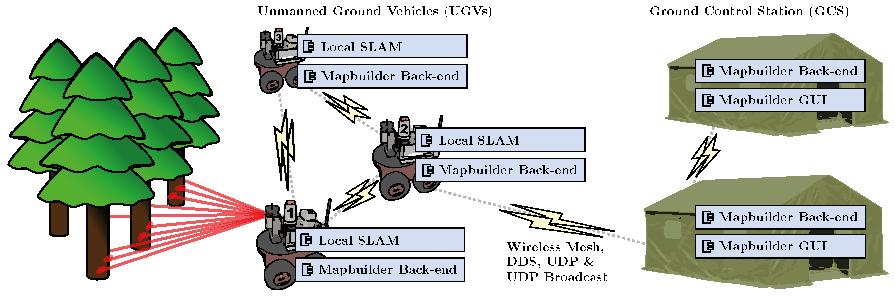
\includegraphics[width=\linewidth]{fig2}
	\caption[MR-SLAM architecture and software development diagram]{The MR-SLAM architecture and software development diagram showing the software components run on the GCS and UGVs.}
	\label{fig:4:mrslam}
\end{figure} 

A typical deployment scenario of the MR-SLAM system is illustrated in Fig.~\ref{fig:4:mrslam}, showing that the back-end is executed across UGVs and GCSs. Each back-end instance stores a local copy of all submaps and constraints, which are then optimised and fused, building global maps; new loop closure constraints between submaps are also searched. Submaps are rectangular grid-maps with dynamically increasing dimensions determined by the LiDAR's maximum range $R$, the environment's shape, and a threshold heuristic described later in this section.

Local SLAM is performed independently on each UGV whereby a single-robot SLAM algorithm builds its own submap by processing its sensor data, which is then broadcasted across the mesh network. Graphical user interfaces (GUIs) are installed on GCS computers to enable operators to view and manipulate global and submaps and interact with pose graphs through a point-and-click interface.

\nomenclature[z-gui]{GUI}{Graphical user interface}

A global grid-map is fused through several overlapping submaps that are obtained from the SLAM algorithms running on each UGV, thereby achieving a distributed map-building sequence. The fusion algorithm searches for overlaps in the grid-maps and subsequently determines if the cells in the global grid-map are occupied, free, or unknown. Each submap initialises with a local coordinate frame on the global frame with its submap pose $p^W_a$, which is estimated through pose graph optimisation in a global Euclidean coordinate frame $W$. Given the UGV pose $r^a_t$ always broadcast relative to $p_a^W$, and that each submap is created with the UGV at its origin, therefore $r^a_0 = [0, 0, 0]^\intercal$, and the UGV's time-varying pose in the global frame is thus:
\begin{align}
r^W_t = p^W_a \oplus r^a_t
\end{align}
Each submap is assigned a 128-bit hexadecimal universally unique identifier (UUID) and exists either in an ``open'' or “closed” state, where they are always created through an “open” state to indicate that an occupied UGV is in the process of building it. Once map building is complete, the submap changes to a “closed” state to render the area immutable and non-traversable by any UGV, only allowing the back-end to update its pose, thereby fusing it onto the global grid-map. Having these states increases the robustness of the MR-SLAM system while ensuring its logic simplicity. A UGV can only occupy a single submap at any given time, and these “open” submaps are often connected to an adjoining “closed” submap. At the creation of a new submap, its map and pose uncertainty is reset. Using this approach enables the system to minimise bandwidth, storage, and redundancy across the MR-SLAM back-end.

\nomenclature[z-uuid]{UUID}{Universally unique identifier}
\nomenclature[a-rab]{$r_a^b$}{UGV pose}  
\nomenclature[a-pab]{$p_a^b$}{Submap pose}  
\nomenclature[r-w]{$W$}{Euclidean coordinate frame}
\nomenclature[s-t]{$t$}{Time}  

Using a ray tracing technique based on~\cite{bresenham_algorithm_1965}, the LiDAR scans obtained while navigating a submap is aligned and fused into a single 2D occupancy grid-map, which maintains an accurate representation of the environment. The LiDAR scans are aligned with scan matching prior to ray tracing to circumvent the accumulation of minor quantisation noise, which is done through a batch rounding of these LiDAR measurements to the nearest grid cell using the grid-map representation.

Aside from quantisation noises, UGV pose uncertainties are also prevalent while it is building a submap. Although a UGV always initialises a new submap with no pose uncertainties, this uncertainty will always accumulate whenever the UGV is manoeuvring, with odometric noise as its main contributor. Therefore, it is more pronounced in larger areas. To solve this problem, the algorithm initialises a new submap whenever this uncertainly surpasses a set threshold, which is determined by comparing the current angular pose uncertainty against the average distance to obstacles in the environment, estimating the amount of “blurring” in distant grid-map cells. Current LiDAR scans will not be fused if a new submap is triggered using this approach; using this heuristic thus minimises distortions entering the submap grid-map, and large distortions that result in misaligned LiDAR scans can be prevented. The algorithm then transfers this accumulated uncertainty's covariance into the new constraint's covariance that is used to connect the old and new submaps through a maximum likelihood estimation.

By assuming an average distance between submaps $D$, the maximum overlap between a sequence of submaps separated by $D$ is given by a ratio:
\begin{align}
\text{Maximum overlap} = \frac{2R}{2R + D}
\end{align}
The MRS yields a maximum submap overlap of 93\%, which implies that the same UGV could create submaps that overlap the same area up to 15 times. This overlapping redundancy is required to allow the distributed back-ends to compare and align map data.

\nomenclature[a-D]{$D$}{Ground distance}  

\subsection{MR-SLAM Architecture}
With reference to Fig.~\ref{fig:4:mrslam}, we have identified the functional roles of the software components as Table~\ref{tbl4:fr}, which illustrates a minimalistic logical design diagram that considers a single UGV and GCS.

\begin{table}[H]
	\caption{Functional requirements of software components}
	\centering
	\label{tbl4:fr}
	\begin{tabularx}{\textwidth}{ p{2cm} X  X X }
		\toprule
		Component        & Input                                                                      & Behaviour                                              & Output                                                                     \\ \midrule
		Local SLAM       & Sensor data (LiDAR, odometry, IMU, GPS)                                    & Performs local SLAM, creates a sequence of submaps     & Broadcasts submap data, constraints, real-time UGV pose estimates          \\
		MR-SLAM back-end & Submap data from all UGVs, submap constraints, ground-truth constraints    & Optimises pose graphs, fuses submap data, searches for & Global or windowed maps, submap pose estimates, submap constraints         \\
		MR-SLAM GUI      & All MR-SLAM messages, GUI events; for example, keystrokes and mouse clicks & Displays global maps, interprets operator commands     & Messages that alter graph structure; for example, ground-truth constraints \\ \bottomrule
	\end{tabularx}
\end{table}

The class diagram in Fig.~\ref{fig:4:cd} illustrates the various message types used by the system for MR-SLAM, which are all derived from the Submap message class. All messages are time-stamped with the source participant's priority and the submap UUID.

\begin{figure}[H]
	\centering
	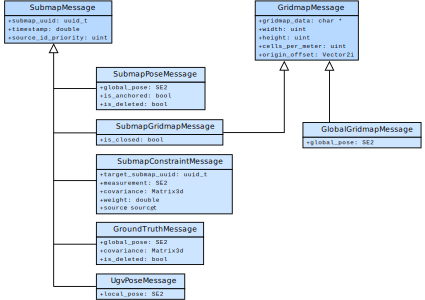
\includegraphics[width=0.9\linewidth]{fig3}
	\caption[MR-SLAM class diagram]{A class diagram showing the MR-SLAM system’s message types and their variables.}
	\label{fig:4:cd}
\end{figure}

For the local SLAM front-end, we use a heuristic-driven EKF-SLAM~\cite{dissanayake_solution_2001} single-robot algorithm that takes all sensor data and outputs submaps, constraints, and real-time pose estimates, which are broadcasted over the mesh network. We have designed this front-end based on the following requirements:
\begin{itemize}
	\item To estimate UGV pose and broadcast in real-time at more than 10 Hz locally, or 1 Hz globally.
	\item To build 10 cm submap grid-maps that are broadcasted at more than 1 Hz locally, or 0.2 Hz globally.
	\item To robustly handle moving objects including human gaits up to 6 km/h.
	\item To handle challenging sensing conditions such as sparse and/or featureless areas.
	\item To detect odometric errors to minimise submap corruption.
	\item To compress submap grid-maps before broadcasting.
	\item To use less than 25\% of total computation and memory footprint.
\end{itemize}
Likewise, the back-end requirements of our MRS are:
\begin{itemize}
	\item To optimise pose graphs robustly and efficiently at less than 5 seconds per iteration.
	\item To output large ($5000\times5000$) grid-maps to the local partition at more than 1 Hz.
	\item To match submaps to generate robust constraints at less than 5 seconds per match.
	\item To broadcast \textbf{SubmapPose} messages globally to maintain decentralised pose graph.
	\item To output \textbf{SubmapPose} updates to the local partition at more than 1 Hz.
\end{itemize}

\subsection{SLAM Implementation}
We apply EKF-SLAM with scan matching which builds submaps by aggregating LiDAR scans at every 20 cm of movement or \ang{20} of rotation, where pose estimation is achieved through an EKF. Scan matching was incorporated to reduce computation requirements by using the described threshold heuristics to decide when a current submap should be closed, which is augmented by a threshold on the percentage of LiDAR returns that are aligned successfully. This method enables the detection of matching failures, especially in sparse environments. EKF is used to estimate the UGV’s pose by initiating each cycle to predict its current pose using the latest wheel odometry and IMU data, which aligns the LiDAR scan against the current submap through scan matching~\cite{censi_accurate_2007}. RANSAC~\cite{martin_a._fischler_random_1981} is also incorporated to reject outliers in the form of moving objects. The EKF and pose estimate is subsequently updated using this scan matching alignment method. Odometric noises that are present in the EKF update are adjusted according to the local ground slope gathered from the pitch and roll measurements from the IMU. An increase in slope leads the module to assume an increase in odometric noise due to wheel slip, thereby switching the filter preference for scan matching over odometry.

\begin{figure}[H]
	\centering
	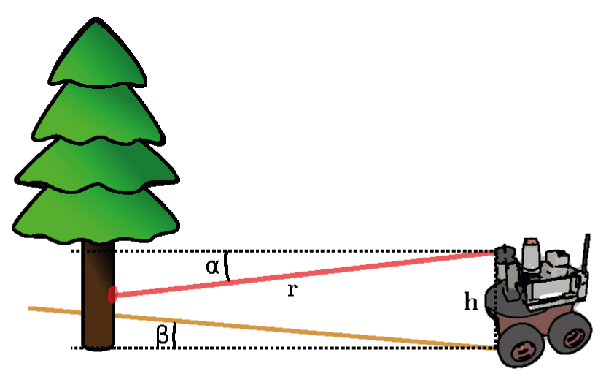
\includegraphics[width=0.6\linewidth]{fig4}
	\caption{Lengths and angles used for calculating the local SLAM prefilter.}
	\label{fig:4:slampf}
\end{figure}

To filter these errors using the IMU, we assume that (1) the terrain inclination is less than $\beta_\mathrm{max}$, and (2) the terrain follows the “Manhattan World”~\cite{coughlan_manhattan_2003} assumption. With reference to Fig.~\ref{fig:4:slampf}, each LiDAR measurement range $r$ is first corrected to account for the declination $\alpha$ from the same measurement as $r\cos\alpha$, whereby an inequality is obtained referencing the height of the LiDAR mounted above the ground $h$.
\begin{align}\label{eqn4:4}
0 < h - r\sin\alpha - r\cos\alpha \cdot \tan\beta_\mathrm{max}
\end{align}
To prevent any measurements from grazing the ground, any instance of $r$ with declination $\alpha$ that dissatisfies \eqref{eqn4:4} is filtered. LiDAR measurements that are corrected and filtered will then be passed to the SLAM algorithm.

\nomenclature[g-a]{$\alpha$}{Declination}    
\nomenclature[g-a]{$\beta$}{Inclination}    
\nomenclature[a-h]{$h$}{Height}  
\nomenclature[a-r]{$r$}{Measurement range [Chapter~\ref{ch:cmrn}]}  


\subsection{UGV/GCS Communications}
Communications between UGVs and GCSs are facilitated through a Wi-Fi mesh network over the IEEE 802.11n standard in a multi-hop configuration over a data distribution system (DDS), which provides a publisher-subscriber framework that provides robust real-time communications. Publishers are separated into partitions which are either global (all participants) or local (within a participant). Global partitions are mostly used to prevent network overloads, as the local partition is used for high-rate inter-process communications, where messages are passed over a shared memory between the front-end, back-end, and other high-level MRS software components.

Messages are broadcasted by the front-end as submaps are closing in the form of compressed grid-map data and the constraint that links the closed submap to the new one. Incomplete grid-maps for open submaps are also broadcasted to visualise real-time global maps; these maps are flagged to indicate that they are not yet immutable. The front-end broadcasts three distinct, time-stamped message types with a fixed DDS buffer size n with varying quality of service (QoS) priorities:
\begin{enumerate}
	\item \textbf{SubmapConstraint} ($n = 1000$) defines the entire pose graph structure. A large buffer size is allocated for the series of small yet vital messages.
	\item \textbf{SubmapGridmap} encodes the actual shape of the environment, constituting most of the MR-SLAM data, which are either open or closed.
	\begin{enumerate}
		\item \textbf{Open} ($n = 0$) grid-maps are disposable as they are periodically broadcasted by the front-end, these are sent to the local partition at the LiDAR’s scan rate.
		\item \textbf{Closed} ($n = 100$) grid-maps have higher priority as they are only transmitted once.
	\end{enumerate}
	\item \textbf{UGVPose} ($n = 0$) are broadcasted frequently in real-time, which stales quickly and is subsequently disposable. These are also sent to the local partition at the LiDAR’s scan rate.
\end{enumerate}
A rendering algorithm ray traces the accumulated LiDAR scans into an empty grid map based on the methods described in~\cite{bresenham_algorithm_1965}. The grid-map data is segregated into $32\times32$ cell tiles that are broadcasted over UDP on a $50:1$ compression ratio.

\nomenclature[z-dds]{DDS}{Data distribution system}
\nomenclature[z-qos]{QoS}{Quality of service}

Likewise, the back-end’s publishing policies are:
\begin{enumerate}
	\item \textbf{SubmapPose}:
	\begin{enumerate}
		\item \textbf{Global Partition} ($n = 0$) does not require delivery guarantees since priority-based filters synchronises this between participants.
		\item \textbf{Local Partition} ($n = 0$) does not require QoS as DDS uses shared memory to delivery real-time submap pose estimates.
	\end{enumerate}
	\item \textbf{SubmapConstraint} ($n = 1000$) is assigned with the highest priority as they define the entire pose graph structure, hence a large buffer size is allocated.
	\item \textbf{GlobalGridmap} ($n = 0$) are delivered through shared memory by DDS in real-time; QoS is therefore not required.
\end{enumerate}

\subsection{Loop Closures}
A loop closure is an event that occurs when a UGV revisits a location it has previously threaded, thereby correcting its accumulated errors. The identification of loop closures occurs between overlapping submap pairs and spatially similar grid maps, which are broadcasted as new constraints that form cycles in the distributed pose graphs, bearing residual errors that require optimisation. The back-end searches for local loop closures between “open” submaps in real-time, especially when multiple UGVs are operating overlapping areas to ensure proper localisation and prevent the accumulation of errors. Using this method enables our system to efficiently accommodate high rates of loop closures and map changes in real-time.

The large number of loop closures generated by the system, as well as the distributed algorithm design, prompted us to utilise the graphics processing unit (GPU) to search for loop closures and merge submaps. Additionally, descriptive spatial relationships between submaps are extracted using a grid-map correlation algorithm on the GPU that calculates likelihood volumes and extracts multimodal Gaussian constraints. Using robust multimodal constraints enables the algorithm to preemptively add loop closures to the pose graph and perform outlier rejection by consensus.

\begin{figure}[H]
	\centering
	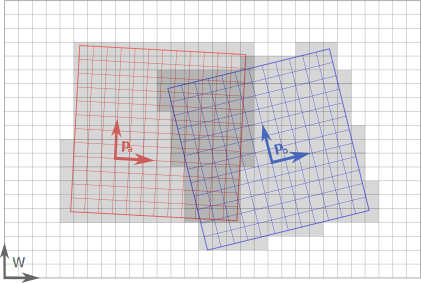
\includegraphics[width=0.7\linewidth]{fig5}
	\caption[Occupancy grid-map fusion]{Occupancy grid-map fusion illustrating two submap grid-maps with their origins $p^W_a$ and $p^W_b$ to be fused onto the global output grid-map $W$ shown as grey grids.}
	\label{fig:4:ogm}
\end{figure}

An overlapping submap pair also initiates an occupancy grid-map fusion algorithm. To achieve the fusion described in Fig.~\ref{fig:4:ogm}, we use a GPU-based approach whereby the algorithm checks for each overlapping cell in the output grid-map and performs a transformation of that cell in its 2D coordinates into the submap’s coordinate frame, subsequently fusing it into the output cell based on the corresponding submap cell value.

To optimise complex multimodal Gaussian constraints, we utilised a continuous mode blending optimisation technique that is based on non-linear least-square approaches and exhibits convergence properties that are representative of the underlying multimodal constraint distributions.

\subsection{SLAM Evaluation}
For the evaluations described here, ten UGVs were deployed to explore an $80\times40$ m environment. The total elapsed time was 36 minutes~\cite{reid_large-scale_2016}. The SLAM routine was completed with minimal user intervention whereby the UGVs autonomously explore the environment while displaying their progress in real-time onto the MR-SLAM system’s GUI. This process follows our approach in~\cite{s._lopes_autonomous_2011} and is illustrated in series across Figs.~\ref{fig:4:slamstart} through~\ref{fig:4:slamend} with timestamps on the upper right corner of the images in minutes and seconds; the total odometry across all UGVs is presented in meters at the lower right corner; UGVs are shown as dots with colour-matched lines showing their trajectories; pose graphs are green with dots, lines, and red triangles representing submap poses, submap constraints, and ground truth constraints, respectively.

The UGVs start at the southeast corner of the warehouse (see Fig.~\ref{fig:4:slamstart}), where two teams split to explore the west and north sections, respectively. Both teams explore independently until a loop closure is evident, as illustrated in Fig.~\ref{fig:4:slammmid}, where the first team is about to exit via the southwestern corner. The exploration forms a total closed path length of 230 m that is measured after the separation of the UGVs in the first room. The final result is presented in Fig.~\ref{fig:4:slamend}. This corresponds to about 70 constraints in the pose graph. Based on 88 samples collected across the surveyed area, the root-mean-square (RMS) error was calculated to be $\approx0.27$ m.

\nomenclature[z-rms]{RMS}{Root-mean-square}

The 2D correlation between each submap in Fig.~\ref{fig:4:mmc} is represented by each slice, with a $\pm3$ m translation variation along with $x$ and $y$-axes at a fixed angular rotation. For example, the middle row represents rotations of $-6$°, $-3$°, 0°, 3°, and 6°, respectively. The 2D ellipses represent three-sigma covariance modes through a Gaussian mixture model that fits the maximum likelihood volume. Occlusions have reduced the overlapping area of occupied cells (black) between the submap pair, and the matcher’s output is mostly dominated by an array of columns in the environment.

\begin{figure}[H]
	\centering
	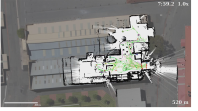
\includegraphics[width=0.8\linewidth]{fig7}
	\caption[SLAM output (starting)]{SLAM output showing the UGVs starting at the southeastern corner of the environment.}
	\label{fig:4:slamstart}
\end{figure}

\begin{figure}[H]
	\centering
	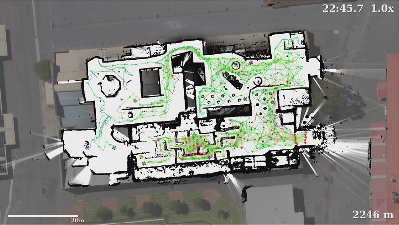
\includegraphics[width=0.8\linewidth]{fig6}
	\caption[SLAM output (loop closure)]{SLAM output showing loop closure between both teams, with the first team about to exit via the southwestern corner.}
	\label{fig:4:slammmid}
\end{figure}

\begin{figure}[H]
	\centering
	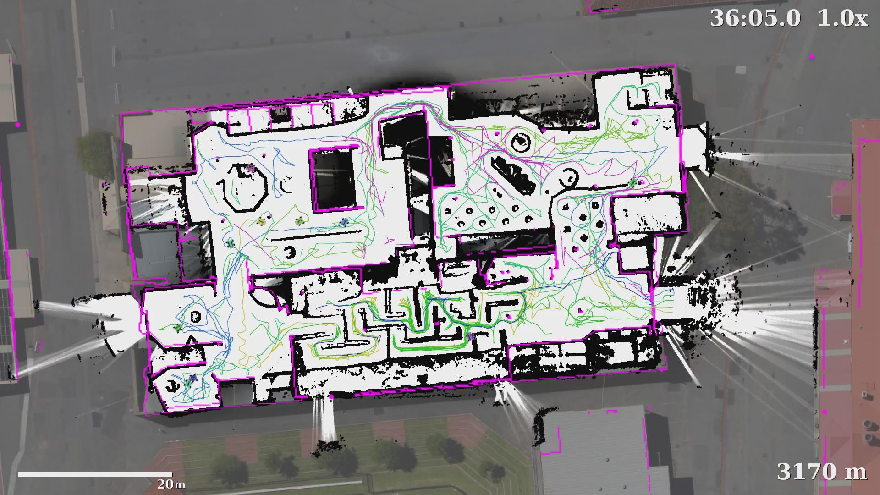
\includegraphics[width=0.8\linewidth]{fig8}
	\caption[Completed global grid-map]{Completed global grid-map with ground truth overlaid in magenta.}
	\label{fig:4:slamend}
\end{figure}

\begin{figure}[H]
	\centering
	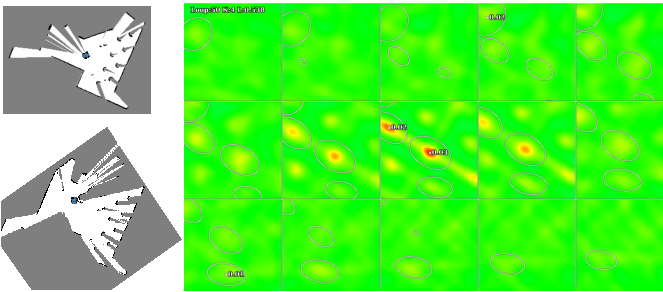
\includegraphics[width=\linewidth]{fig9}
	\caption[Multimodal constraint output]{Example of multimodal constraint output with perceptual aliasing. The correlation results for a test area with perceptual aliasing that was caused by repetitive geometry. It shows an overlapping submap pair (left) along with 15 slices through their constraint likelihood volume.}
	\label{fig:4:mmc}
\end{figure}

\section{Visual Odometry}\label{sec:4:vo}
While some effort was made to circumvent wheel slip accumulation in Section~\ref{sec:4:cln}, other works have demonstrated that visual odometry is often an effective solution to this problem~\cite{aqel_review_2016}. In the case of the MRS, this can be incorporated with no hardware or sensor modifications. Taking advantage of the system’s software scalability, this was programmed on top of the existing software with minimal impact to the overall system.

\subsection{Visual Odometry Method}
As with most practical visual computing applications, the implementation of visual odometry in the real world comes with its own sets of challenges~\cite{zhao_visual_2015}. Environmental dynamics, including variations in seasons, light intensity, sensor occlusions, and motion blurs are capable of distorting visual odometry results that will in turn affect its accuracy. Our application will require that the algorithm is robust enough to withstand the environmental variations present in an urban outdoor environment.

Visual odometry works by tracking either features or appearances in the image frame~\cite{scaramuzza_visual_2011, yousif_overview_2015} with appearance-based approaches usually resulting in more accurate tracking but at the cost of computation complexity. The decentralised nature of the MRS dictates visual odometry to be performed on each robot’s computer as a separate subroutine to MR-SLAM, thereby requiring a feature-based method to be implemented. While visual odometry can be applied across different image features and many feature-based methods do exist~\cite{yousif_overview_2015, chien_when_2016}, oriented FAST and rotated BRIEF (ORB) features~\cite{e._rublee_orb:_2011} were found to be most compatible for the system due to the following:
\begin{itemize}
	\item ORB features achieve a compromise between accuracy and system footprint. In other words, it is adequately accurate for the MRS application while having computation requirements that are low enough to be run on the individual robots.
	\item ORB features were proposed and tested in urban environments, whereby the structured appearance of urban environments enabled ORB features to be extracted effectively, especially on the KITTI benchmark suite~\cite{geiger_are_2012}.
\end{itemize}
Based on these rationales, an algorithm based on ORB-SLAM~\cite{mur-artal_orb-slam2:_2017} was implemented as the visual odometry solution for this system. Once a camera has been corrected for radial distortions, the algorithm tracks ORB features across each frame to determine the displacement of each tracked pixel at every new frame, thereby localising the robot. It functions as a separate thread and routine on the onboard computer to minimise any interference to the other routines running on the robots.

As visual odometry is effectively a visual SLAM algorithm without loop closures, the MRS' implementation of ORB-SLAM is hence used purely for odometry; loop closures and SLAM are still managed by the LiDAR-based front-end, independent from visual odometry.

\subsection{Visual Odometry Evaluation}\label{sec:4:voe}
Evaluations for visual odometry were performed on individual UGVs as the implementation was fully decentralised. To optimise for performance and to reduce redundancy, a modified version of ORB-SLAM2 was proposed whereby all subroutines related to visual SLAM, such as loop closure detection and mapping, are removed. By delegating all SLAM routines to the LiDAR-based front-end, this modification yielded a 120\% increase in performance gain in terms of output frame-rate. Additionally, maps created through the LiDAR-based front-end delivers more accurate point cloud measurements as compared to our monocular camera setup, and a LiDAR-based map requires lower computation and storage requirements than a vision-based solution.

ORB-SLAM2 achieves visual odometry by tracking ORB features, as shown in Fig~\ref{fig:4:orb1}. This evaluation was performed in an outdoor environment with unconstrained lighting conditions using a calibrated monocular camera. Tests were carried out while driving along a 220 m path while generating its trajectory as shown in Fig.~\ref{fig:4:orb2}, where it is indicated in blue; the black dots represent previously tracked ORB features, whereas the red dots represent the features that are currently tracked.

\begin{figure}[H]
	\centering
	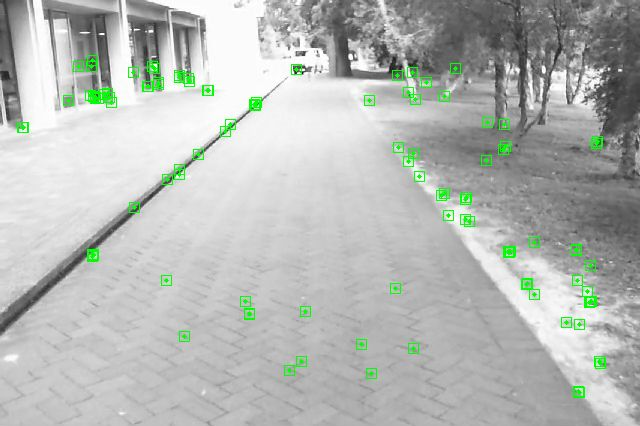
\includegraphics[width=0.8\linewidth]{fig10}
	\caption[Tracked ORB features]{ORB features tracked by ORB-SLAM2 as shown in bounding boxes.}
	\label{fig:4:orb1}
\end{figure}

\begin{figure}[H]
	\centering
	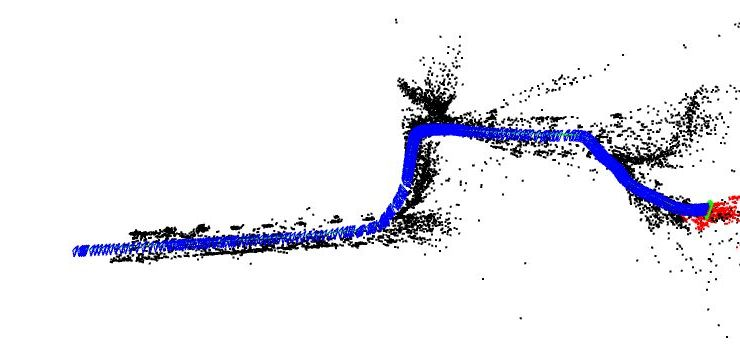
\includegraphics[width=0.8\linewidth]{fig11}
	\caption[ORB-SLAM2 trajectory]{Trajectory measured using ORB-SLAM2 for dead reckoning (blue), previously tracked ORB features (black) and presently tracked ORB features (red).}
	\label{fig:4:orb2}
\end{figure}

\section{Semantic Segmentation}\label{sec:4:semseg}
The incorporation of semantic segmentation into the MRS enables navigation to be supplemented with scene understanding and object classification. Semantic segmentation is a deep learning process that classifies each pixel in an image frame according to the object class it belongs to. This is especially useful in complex environments with multiple objects, with little uniformity in pose, features, and illumination.

\subsection{Semantic Segmentation Method}
For the semantic segmentation application of the MRS, SegNet~\cite{badrinarayanan_segnet:_2017} was selected based on its high compatibility and ease of implementation. The architecture of SegNet uses a convolution encoder and decoder setup that classifies objects from one of the following classes: sky, building, column-pole, road-marking, road, pavement, tree, sign-symbol, fence, vehicle, pedestrian and bicyclist; with a class average classification accuracy of 65.9\%~\cite{badrinarayanan_segnet:_2017}. This MRS uses SegNet whereby pedestrians, vehicles, buildings, vegetation, and pathways are classified as illustrated in Fig.~\ref{fig:4:ss1}, and are subsequently classified into static and dynamic objects.

Static objects are stationary (with stationary positions), while dynamic objects are moving (with time varying positions). It is important for an MR-SLAM system to differentiate static and dynamic objects to devise proper navigational reactions to the environment. For example, static objects such as buildings and vegetation are permanent placements in the environment; these objects will be mapped by the MR-SLAM algorithm as part of the environment. Conversely, dynamic objects such as pedestrians and vehicles are in motion or are temporary placements in the environment; these will not be mapped by the MR-SLAM algorithm. Overall, this process of differentiating object types will ultimately result in higher mapping accuracy, especially when the ground truth does not contain dynamic objects.

The recognition of dynamic objects also enables the system to estimate the motion of a specific moving object. In other words, by segregating moving vehicles or pedestrians within an image frame, the LiDAR can then be utilised to estimate the motion and trajectory of the said object. This enables the robot to actively perform obstacle avoidance according to its motion, which can be implemented by comparing the robot’s current speed against the LiDAR measurements on the classified dynamic object based on the image frame.

\subsection{Semantic Segmentation Evaluation}
Like visual odometry, semantic segmentation was also implemented in a decentralised approach onto individual UGVs. A Caffe~\cite{jia_caffe:_2014} implementation of SegNet is installed onto the individual UGVs, which enables pixelwise object classification that corresponds to LiDAR measurements at that time instance, which can be any of 12 classifiable classes. We subsequently separate these classes into static and dynamic classes. For example, bicycles, pedestrians, and vehicles are dynamic, whereas buildings, fences, pavement, poles, road, road markings, road signs, vegetation, and sky are static. By matching the position of the classified pixel at the $x$-axis against that of the LiDAR on a fixed $y$-plane, dynamic objects can therefore be segregated and tracked using the LiDAR for motion detection. Objects in motion will be compared against the trajectory of the UGV to ensure that there is no impending collision. These dynamic objects will also be ignored as part of the SLAM routine so that it does not become mapped as part of the environment.

\begin{figure}[H]
	\centering
	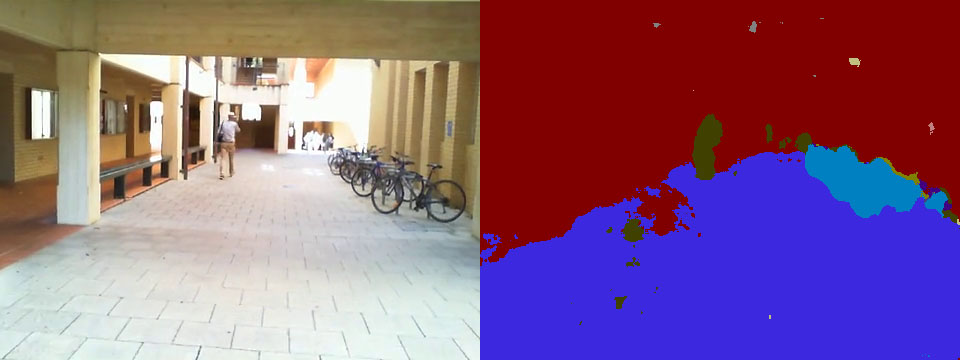
\includegraphics[width=0.8\linewidth]{fig12}
	\caption[SegNet output 1]{SegNet output showing segmented pedestrian (olive), bicycles (light blue), pathway (blue) and building (red).}
	\label{fig:4:ss1}
\end{figure}

Fig.~\ref{fig:4:ss1} was captured while navigating along the path as described in Section~\ref{sec:4:voe}. The parked bicycles on the right side and the pedestrians in the distance were properly segmented as dynamic objects, and the building and pavement as static objects. Several false detections are present due to variations in lighting and image quality, which accounts for 2.83\% of the total pixels classified on the pavement region.

\begin{figure}[H]
	\centering
	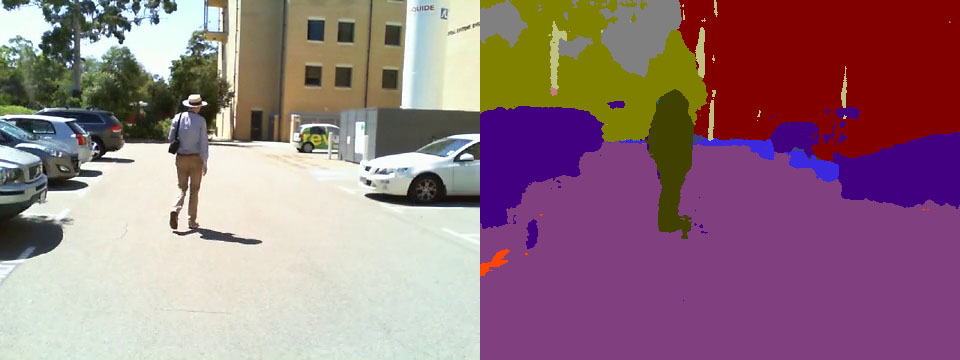
\includegraphics[width=0.8\linewidth]{fig13}
	\caption[SegNet output 2]{SegNet output from a parking area showing segmented road regions (purple), road markings (orange), and poles (yellow).}
	\label{fig:4:ss2}
\end{figure}

Fig.~\ref{fig:4:ss2} was also captured on the same path. While driving on roads, the road region and markings are properly classified along with the electric poles, vehicles, and pedestrians. Uniform lighting resulted in accurate classification accuracy with 0.69\% of all pixels falsely classified.

\section{Conclusion}
In this chapter, we have presented a decentralised multi-robot system for SLAM in urban outdoor environments together with visual odometry and semantic segmentation techniques. The vision-based methods can be used as an alternative to LiDAR-based localisation and object classification and may lead an overall cheaper and more powerful environmental perception system. We have presented an on-line, distributed, and decentralised MR-SLAM system that has proven to be resilient against environmental dynamics such as variations in lighting, terrain, pose, and moving objects. Evaluation results have confirmed the feasibility of using visual odometry as a viable solution to the odometry problem in an MRS, while semantic segmentation is a robust solution to object classification and scene understanding. Practical applications of this system can include search-and-rescue or reconnaissance missions in uncharted or hazardous environments, where detailed maps can be built quickly and accurately using a swarm of robots that are easily deployable, while being robust enough to cater to changes in the environment and hardware setup.
%!TEX root = ../thesis.tex

\chapter[Semantic Segmentation for Road and Lane Detection]{Implementation of Semantic Segmentation for Road and Lane Detection on an Autonomous Ground Vehicle with LiDAR}
\label{ch:semseg}

\ifpdf
	\graphicspath{{Chapter5/Figs/Raster/}{Chapter5/Figs/PDF/}{Chapter5/Figs/}}
\else
	\graphicspath{{Chapter5/Figs/Vector/}{Chapter5/Figs/}}
\fi

While current implementations of LiDAR-based autonomous driving systems are capable of road following and obstacle avoidance, they are still unable to detect road lane markings, which is required for lane keeping during autonomous driving sequences. In this paper, we present an implementation of semantic image segmentation to enhance a LiDAR-based autonomous ground vehicle for road and lane marking detection, in addition to object perception and classification. To achieve this, we installed and calibrated a low-cost monocular camera onto a LiDAR-fitted Formula SAE Electric car as our test bench. Tests were performed first on video recordings of local roads to verify the feasibility of semantic segmentation, and then on the Formula SAE car with LiDAR readings. Results from semantic segmentation confirmed that the road areas in each video frame were properly segmented, and that road edges and lane markers can be classified. By combining this information with LiDAR measurements for road edges and obstacles, distance measurements for each segmented object can be obtained, thereby allowing the vehicle to be programmed to drive autonomously within the road lanes and away from road edges.

\section{Introduction}
The Renewable Energy Vehicle (REV) Project at the University of Western Australia conducts research into electric vehicles, vehicle automation and autonomous driving systems. Recent projects include the development of an Autonomous Formula SAE Electric car~\cite{t._drage_integration_2014}. This vehicle is an open-wheeled, electric drive race car, with electronic drive-by-wire and electromechanical brake/steering actuation. The vehicle serves as a compact, flexible test-bed for sensor testing and the development of autonomous driving algorithms.

\nomenclature[z-rev]{REV}{(The) Renewable Energy Vehicle (Project)}
\nomenclature[z-sae]{SAE}{Society of Automotive Engineers}


Prior research has been conducted on road and road edge detection through optical systems~\cite{p._y._shinzato_road_2014}, radar~\cite{guo_road_2015} as well as using Light Density and Ranging (LiDAR) sensors such as in the winning entry in the 2007 DARPA Urban Challenge~\cite{zhang_lidar-based_2010}. The methodology described in~\cite{nikolova_segmentation_2000} utilises a feature-extraction algorithm while other algorithms such as~\cite{zhao_curb_2012} rely on the presence of curbs and seek to identify and track curbs as features in the LiDAR data. More recently, there has been an increase in the use of cameras to achieve this~\cite{alkhorshid_road_2016}, giving rise to visual road detection. Methodologies to achieve this include feature extraction and classification~\cite{alkhorshid_road_2016}, horizon and vanishing point detections~\cite{p._y._shinzato_fast_2012}, and artificial neural networks (ANNs)~\cite{abbas_novel_2016}.

\nomenclature[z-ann]{ANN}{Artificial neural network}

The problem of path-finding can be described as: ``Given a start state, a goal state, a representation of the robot and a representation of the world, find a collision-free path that connects the start with the goal satisfying the system constraints''~\cite{lavalle_planning_2006}. In mobile robotics, a proven method to obtain the requisite “representation of the world” is via the use of LiDAR data to generate a virtual map in real-time both as the sole sensor~\cite{liu_mobile_2012} and in conjunction with data from additional sensors~\cite{mengyin_multiple_2014}. Similar LiDAR based map building approaches have been shown to be suitable for outdoor terrain~\cite{d._m._cole_using_2006}. These generated maps vary from simple two-dimensional maps suitable for basic path planning consisting of traversable regions, obstacles and unexplored regions~\cite{hao_path_2014} to more complex three-dimensional maps from which sophisticated cost maps are generated~\cite{j._gillula_how_2006}. A more detailed map can be built by supplementing the camera in addition to LiDAR. These additional details can include a combination of vehicle detection and classification~\cite{f._zhang_vehicle_2014}, road sign recognition~\cite{gudigar_review_2016}, and scene recognition~\cite{yang_scene_2015}. 

Visual cameras and LiDAR are often incorporated in autonomous driving systems. Works that combine LiDAR and camera sensors for autonomous driving include the approach from Zhang, Clarke and Knoll~\cite{f._zhang_vehicle_2014}, where they have proposed the fusion of LiDAR and the camera as a compromise for each sensor's drawbacks, with LiDAR providing range information, and the camera identifies objects and scenes. The authors achieved low false alarm rates and a high detection rate for vehicles in urban environments.  A similar fusion of multiple LiDAR, radar, and camera sensors to achieve object detection and tracking was proposed by Cho et al.~\cite{h._cho_multi-sensor_2014}. By tracking pedestrians and vehicles, the system could detect and track vehicles from 150 m away, and pedestrians and cyclists within a 20 m radius. To the best of our knowledge, works that incorporate semantic segmentation onto a LiDAR-based autonomous ground vehicle has not been established at the time of writing. 

Our work is an enhancement to the work done by Drage, Churack and Br\"aunl~\cite{drage_lidar_2015}, where we have proposed a LiDAR-based road edge detection approach on the same vehicle. Our algorithm could detect road curbs and edges by measuring the differences in surface smoothness, which in turn allows the positioning of road edges and curbs.

\section{Implementation}
This section describes the addition of visual perception to the LiDAR-based autonomous SAE car as described in~\cite{drage_lidar_2015}, which includes sections that describe our testing environment, and its applicable procedures to achieve visual autonomous driving. By mounting a monocular camera onto the chassis of the vehicle,  above the LiDAR (see Fig.~\ref{fig:5:cam}), road recognition and obstacle detection are achieved using semantic segmentation. This camera supplements the LiDAR, where the LiDAR is responsible for providing distance measurements for objects and road edges detected by the camera. Semantic segmentation was achieved using SegNet~\cite{badrinarayanan_segnet:_2017}, a convolutional neural network (CNN) architecture for semantic segmentation that is often used for road scenes. Its architecture uses an encoder-decoder network that is followed by a pixelwise classification layer, where the encoder and decoder networks consist 13 convolutional layers each. The Caffe~\cite{jia_caffe:_2014} implementation of SegNet is used for this project. To interface the sensors for autonomous driving, SegNet is installed onto an Nvidia Jetson TX1~\cite{nvidia_corporation_embedded_2017-1}, and the LiDAR interfaces directly to a Raspberry Pi 3~\cite{raspberry_pi_foundation_raspberry_2017}, which drives a control system. A GPS module and an inertial measurement unit (IMU) module also connects to the Raspberry Pi 3 for positioning and localisation. 

The LiDAR system used in this project consists of an ibeo Lux automotive LiDAR with specifications as shown in Table~\ref{tablidar}. This sensor utilises reflected infra-red light to measure distance (via time-of-flight) and can build a 3D point cloud by scanning horizontally in four vertical layers. The ibeo sensor has sophisticated internal data processing functionality including object detection and classification. Data is delivered using TCP/IP over an Ethernet connection and includes scan data in polar coordinates and object data in $x$-$y$ coordinates referenced to the sensor.

\begin{figure}[H]
	\centering
	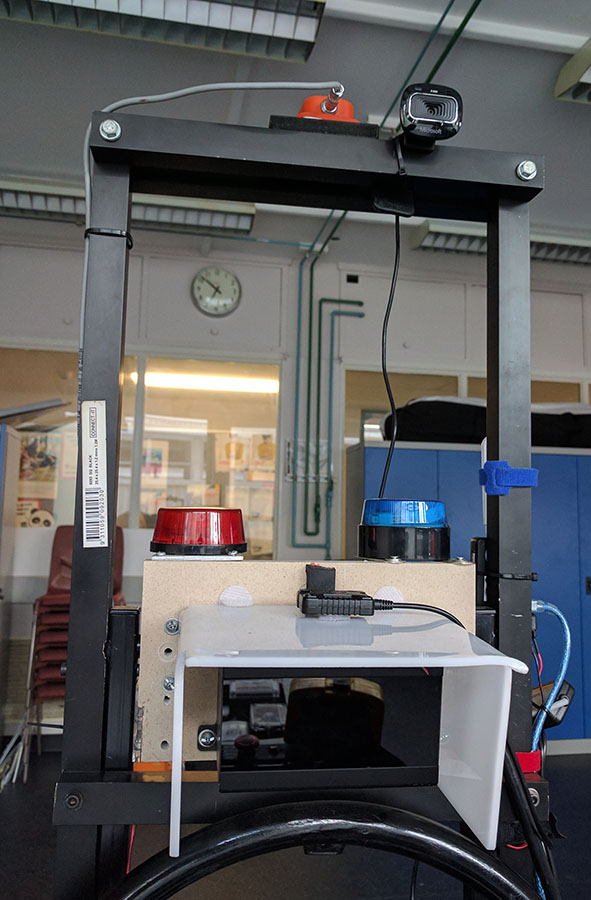
\includegraphics[width=0.35\linewidth]{cammount}
	\caption[Camera mounting location]{The camera is mounted above the LiDAR system from~\cite{drage_lidar_2015}, beside the IMU.}
	\label{fig:5:cam}
\end{figure}

\begin{table}[H]
	\caption{LiDAR Characteristics}
	\label{tablidar}
	\centering
	\begin{tabularx}{0.85\textwidth}{>{\raggedright}p{3cm} X}
		\toprule
		\bfseries Specification & \bfseries Value\\
		\midrule
		Technology & Time of flight (output of distance and echo pulse width)\\
		Range & 200 m\\
		Field of View (Horiz / Vert) & \ang{85} / \ang{3.2}\\
		Layers & 4\\
		Echo Detection & 3 measurements per pulse\\
		Update Rate & Up to 50Hz\\
		Accuracy & 10cm\\
		\bottomrule
	\end{tabularx}
\end{table}

The following subsections describe the process of achieving visual autonomous driving for our project using semantic segmentation with respect to its application environment and its driving sequences.

\subsection{Application Environment}
SegNet was tested within the grounds of the University of Western Australia (UWA), which is the same location that the LiDAR system was tested in~\cite{drage_lidar_2015}. The roads within UWA offers a similar drive environment to standard suburban roads. These single carriageway roads are of low traffic density, with views of pedestrians, faculty buildings, and vegetation for SegNet to recognise and segment. As a feasibility test, we also tested SegNet off a car-mounted dashcam recording while driving on local roads. 

This application environment was selected to test the suitability of using SegNet for autonomous driving locally and to gauge the visual autonomous navigation performance of the vehicle. To achieve a successful autonomous drive using SegNet on the vehicle, road edges and lane markings must be properly recognised, before the application can be subsequently expanded onto a road-licensed vehicle.

It should be noted that our initial implementation uses the trained dataset from the University of Cambridge, CamVid~\cite{badrinarayanan_segnet:_2017}. This dataset was recorded in the City of Cambridge, England. Like most British cities, Cambridge's roads are often narrow, with dense buildings by the side. There is also a large pedestrian population due to it being an academic city. Comparatively, roads in Perth are generally wider, with a sparser build-up density than Cambridge. Its low population density means that there are fewer road pedestrians as compared to Cambridge. The ground terrain around Perth is mostly flat, with long sunshine hours. This means that one can generally expect excellent road visibility on Western Australian roads on most days. However, during poor visibility and night time drives, suburban roads around Perth are generally poorly lit, which may affect road segmentation accuracy. By testing this dataset, we will subsequently contemplate on the need to record and use a dataset from Perth for more accurate segmentation results.

\subsection{Autonomous Driving Procedures}
To use SegNet's output for autonomous driving, we assume that the car begins with a position in the middle of the road lane and that the road incline is flat. By mounting the camera at a fixed position on the car, the central driving position of the car can be obtained, along with distance measurements from the road edges to the left and right sides of the car. With the camera, this is done by identifying and segregating a fixed trapezoidal image region that encapsulates the road segment, which is then transformed into a birds-eye view perspective to obtain vehicle's position with respect to the road's centre. By scaling the road width according to the Australian standards of 3.3--3.5 m, along with the detected road edges and/or lane markings on SegNet's output, the distance from the vehicle's centre to the left and right road edges/lanes can is obtained as Fig~\ref{fig:5:4pane}, with its confidence value determined by the successful detection of road edges or lane markings. From these three sections distance thresholds for the left and right edges or lane markers distances for the car to autonomously centre itself on the road while driving. We call this road centring. In the event where lane markers are not found, road edges will be used instead.

To perform road centring, the car must steer itself in the opposite direction when it crosses the distance threshold to either the left or right road edge/lane markers. The distance from the car to the road edges or lane markers are constantly analysed. If the car is too close to the edge or lane marker, the road centring algorithm will then send commands to the drive system to steer away from the edges with fine adjustments, until the car is cleared from the distance threshold.

\begin{figure}[H]
	\centering
	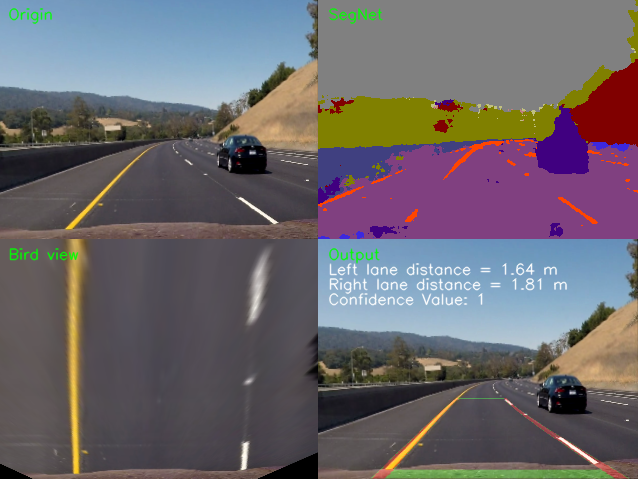
\includegraphics[width=0.8\linewidth]{4pane}
	\caption[Lane distance measurements with SegNet]{Lane distance measurements with SegNet's output on Udacity's Self-Driving Car Nanodegree recording~\cite{udacity_self-driving_2017} as the input in ``Origin''.}
	\label{fig:5:4pane}
\end{figure}

\section{Testing and Evaluations}
\subsection{Methodology} \label{secmethod}
Testing begins with the calibration of the camera, where distance measurements in the real world will be represented in pixel ratios on SegNet's output. Here, we calibrated a Microsoft LifeCam HD-3000 camera. This was done by measuring the distances between road bollards in front of the parked vehicle on the road as illustrated in Fig.~\ref{fig:5:front}.

\begin{figure}[H]
	\centering
	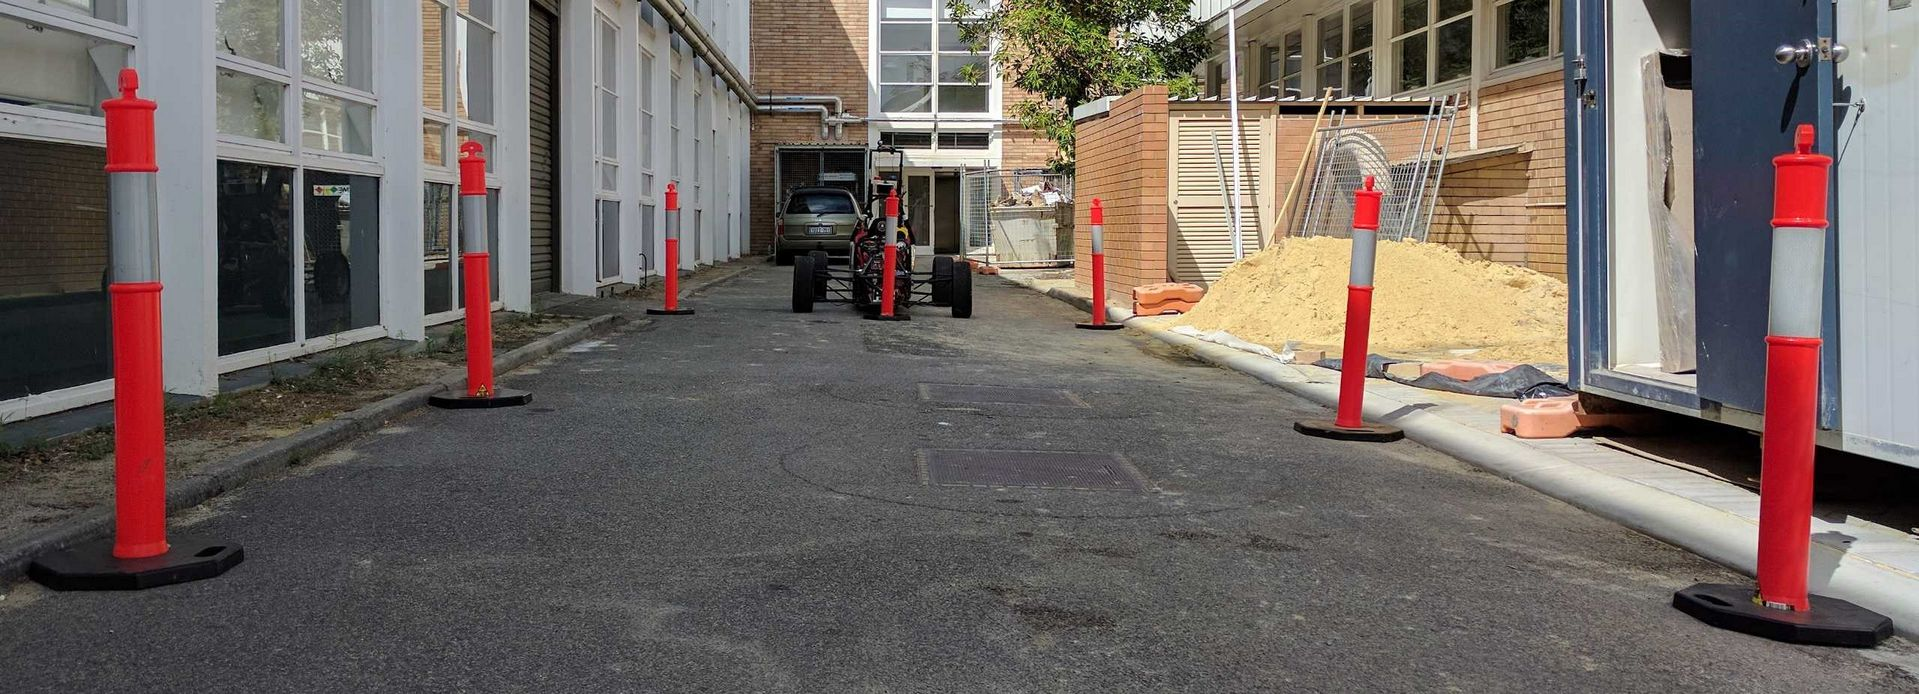
\includegraphics[width=0.8\linewidth]{front}
	\caption[Bollards' position with reference to the car]{Photo illustrating the bollards' position with reference to the car in the centre.}
	\label{fig:5:front}
\end{figure}

The bollards are placed a three-row formation to allow distance measurements from two-point distances on the frame. The first row of bollards on the car establishes the starting distance, with the centre bollard measuring the distance from the camera to the front of the car, while ensuring that the camera is pointed to the centre of the car. All distances are measured from the base at the centre of each bollard. Subsequently, a topological representation of the measurements can be illustrated in Fig.~\ref{fig:5:distances}, which is then represented again in the camera frame in Fig.~\ref{fig:5:bollards}. These measurements are verified with the LiDAR plot at that position as illustrated in Fig.~\ref{fig:5:lidarb}, where the bollards (represented as dot plots) are clearly present around the 2 m, 8 m and 10 m mark on the y-axis. From Fig.~\ref{fig:5:bollards}, each image pixel was calculated to represent 17 mm and 23 mm when measured from 8.5 m and 11.6 m respectively from the camera, and that a level road will converge at around \ang{41} on the camera frame.

The LiDAR readings complement SegNet's output for road edge detection, whereby we use our Kalman Filtered Linear Regression Model as described in~\cite{drage_lidar_2015}. Our algorithm minimises the square residuals between the fit line $y$ and the data ($x_i$, $y_i$), where the most suitable data line will be obtained for a given data set, and its success measured by the product-moment correlation coefficient $r$. The slope $b$ and $r$ values are given as~\eqref{eqn:5:1}.
\begin{subequations}
	\label{eqn:5:1}
	\begin{align}
		y &= (\bar{y}-b\bar{x})+bx \\
		r &= \frac{s_{xy}}{s_x s_y}%x = \sum\limits_{i=0}^{z} 2^{i}Q
	\end{align}
\end{subequations}
where:
\begin{subequations}
	\label{eqn:5:2}
	\begin{align}
	b &= \frac{s_{xy}}{s_x}^2\\
	s_{xy} &= \frac{\sum_{i=1}^{n} x_i y_i}{n}-\bar{x}\bar{y} \\
	{s_x}^2 &= \frac{\sum_{i=1}^{n} {x_i}^2}{n}-\bar{x}^2 \\
	{s_y}^2 &= \frac{\sum_{i=1}^{n} {y_i}^2}{n}-\bar{y}^2
	\end{align}
\end{subequations}

\nomenclature[a-x]{$x$}{$x$-coordinate (Cartesian system)} 
\nomenclature[a-y]{$y$}{$y$-coordinate (Cartesian system)} 
\nomenclature[a-r]{$r$}{Product-moment correlation [Chapter~\ref{ch:semseg}]} 
\nomenclature[a-b]{$b$}{Slope} 

\begin{figure}[H]
	\centering
	\def\svgwidth{0.4\linewidth}
	\input{Chapter5/Figs/PDF/distances.pdf_tex}
	\caption[Topological distance between bollards and car camera]{The topological distance between bollards (dots) and the camera on the car (shaded square).}
	\label{fig:5:distances}
\end{figure}

\begin{figure}[H]
	\centering
	\def\svgwidth{0.6\linewidth}
	\input{Chapter5/Figs/PDF/bollards.pdf_tex}
	\caption{Frame captured from the vehicle's camera for distance calibration.}
	\label{fig:5:bollards}
\end{figure}

\begin{figure}[H]
	\centering
	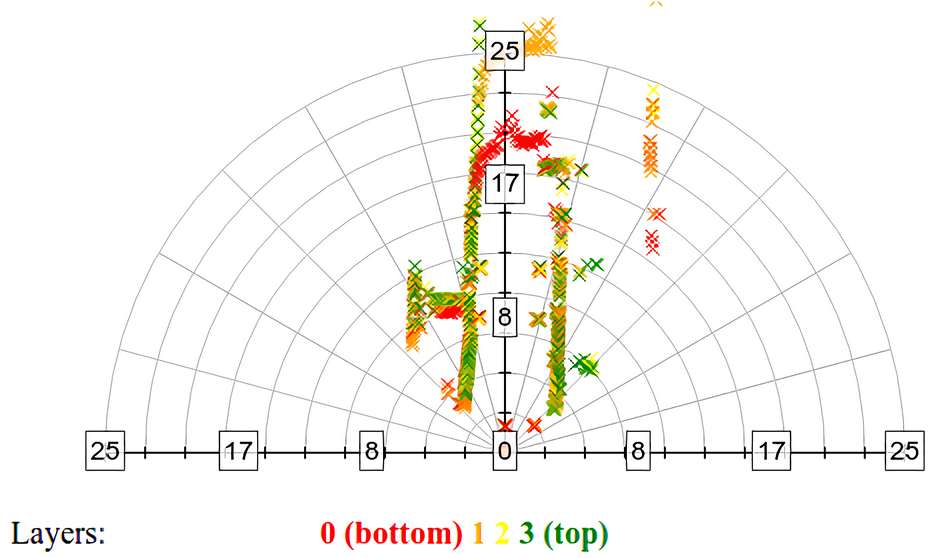
\includegraphics[width=0.8\linewidth]{bollardslidar}
	\caption[Calibration LiDAR plot]{LiDAR plot showing the detected road edges and the bollards' positions from the car where Fig.~\ref{fig:5:bollards} was captured. The graph axes measure distances in metres.}
	\label{fig:5:lidarb}
\end{figure}

With a calibrated camera and LiDAR, the SAE car was driven around the application environment while the camera is recording. The recorded camera footage was used as an input for SegNet. For testing purposes, these footages were processed off-line with SegNet running off an Nvidia GTX Titan X GPU with a 480 by 360-pixel resolution, which resulted in a segmented image output at a consistent 10 frames per second (FPS) sampled at each video frame. This framerate is consistent with the visual autonomous driving results published by Nvidia in~\cite{bojarski_end_2016}, making it adequate for autonomous driving. Further work is required for real-time on-line processing on the Jetson TX1. Likewise, LiDAR plots are also recorded during the duration of the drive, where timestamps are used to synchronise outputs.

\nomenclature[z-fps]{FPS}{Frames per second}

\subsection{Results and Discussions}
Results from semantic segmentation are presented first on open roads with a dash cam recording, and then on the UWA campus ground with the SAE car. Image results in this section are presented with the left image showing segmentation input, and the right image showing its output through SegNet. In the case of false detections, they will be measured in their pixel accuracy (PA). This is done by finding the percentages of road regions, which is done by counting the number of falsely detected pixels $p_{ii}$ against the total number of pixels $k$ in the road region $p_{ij}$ for that image frame:

\begin{align}
\mathrm{PA} = \frac{\sum_{i=0}^k p_{ii}}{\sum_{i=0}^k \sum_{j=0}^k p_{ij}}
\end{align}

\nomenclature[z-pa]{PA}{Pixel accuracy}
\nomenclature[a-p]{$p$}{Classified pixel} 

Segmentation results from the open road testing from the dashcam footage yielded consistently favourable results, as shown in Fig.~\ref{fig:5:road}. Recordings were captured on a clear day, driving on a low traffic dual carriageway. The road region is accurately segmented with negligible false detections. In addition to the road and its markings, SegNet can detect and segment the speed limit sign and the right turn sign ahead. All vehicles and vegetation were also properly detected and segmented. The minor false detections in the sky region are due to the CamVid dataset being trained on a cloudy day, but this should not affect road detection accuracy in any way. This result confirms the feasibility that a CamVid-trained SegNet can be implemented for autonomous driving in the Perth metro area.

\begin{figure}[H]
	\centering
	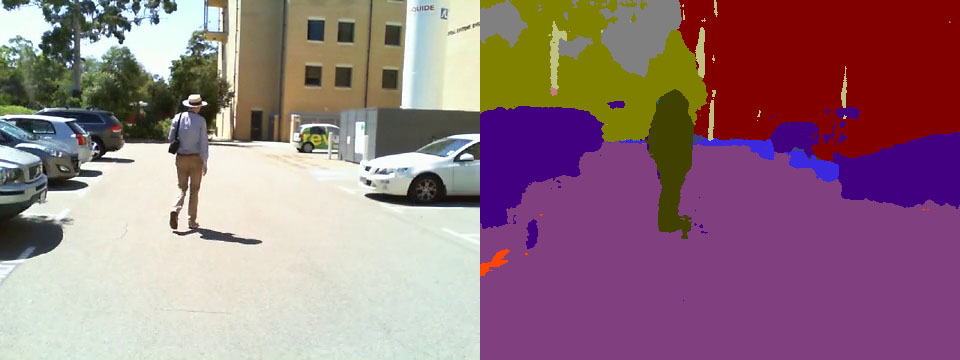
\includegraphics[width=0.8\linewidth]{segnet}
	\caption[SegNet results on a Perth dual carriageway]{SegNet's input (left) and output (right) for a dual carriageway in the Perth metro area.}
	\label{fig:5:road}
\end{figure}

Tests were subsequently performed on the SAE car for a vision-LiDAR-based implementation. Here, runs on campus grounds were recorded using the camera while manually driven on the SAE car following a predetermined route on campus. The car traversed across roads and pavements and the segmentation results are as follows.

\begin{figure}[H]
	\centering
	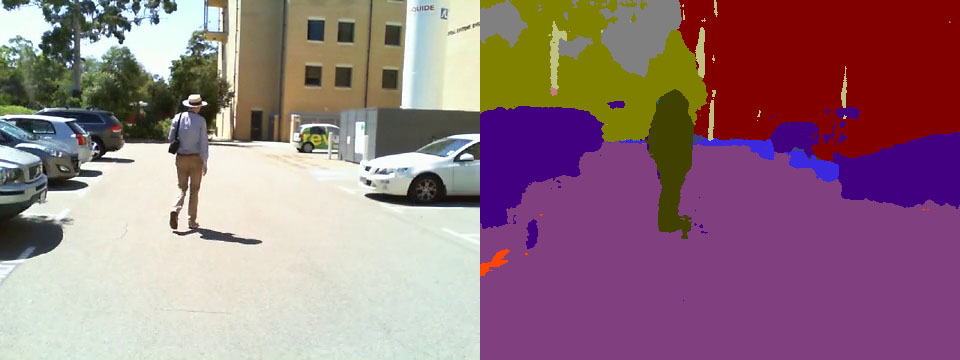
\includegraphics[width=0.8\linewidth]{2}
	\caption{Segmentation results from a parking area on campus grounds.}
	\label{fig:5:carpark}
\end{figure}

\begin{figure}[H]
	\centering
	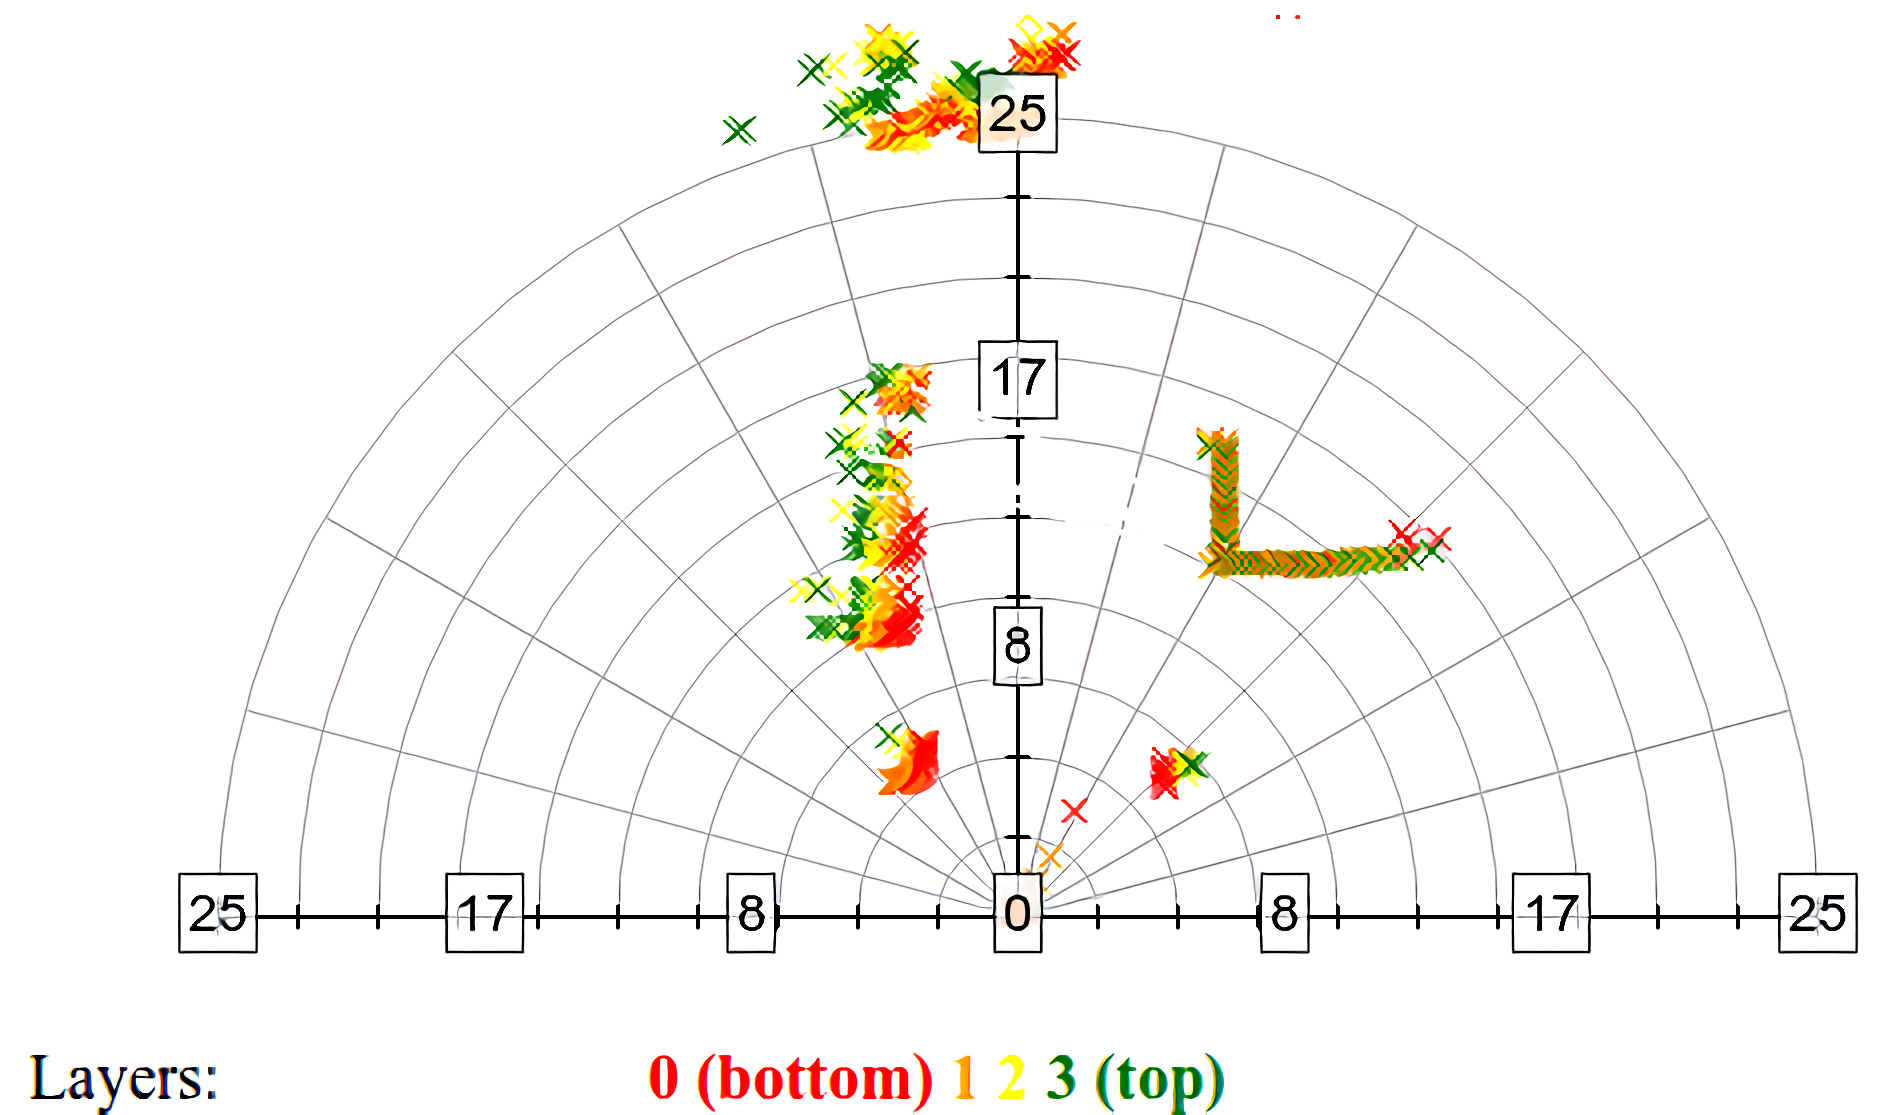
\includegraphics[width=0.8\linewidth]{luxplot}
	\caption[LiDAR plot at the position of Fig.~\ref{fig:5:carpark}]{LiDAR plot showing the detected parked vehicles at the position where Fig.~\ref{fig:5:carpark} was captured. The graph axes measure distances in metres.}
	\label{fig:5:lidar}
\end{figure}

\begin{figure}[H]
	\centering
	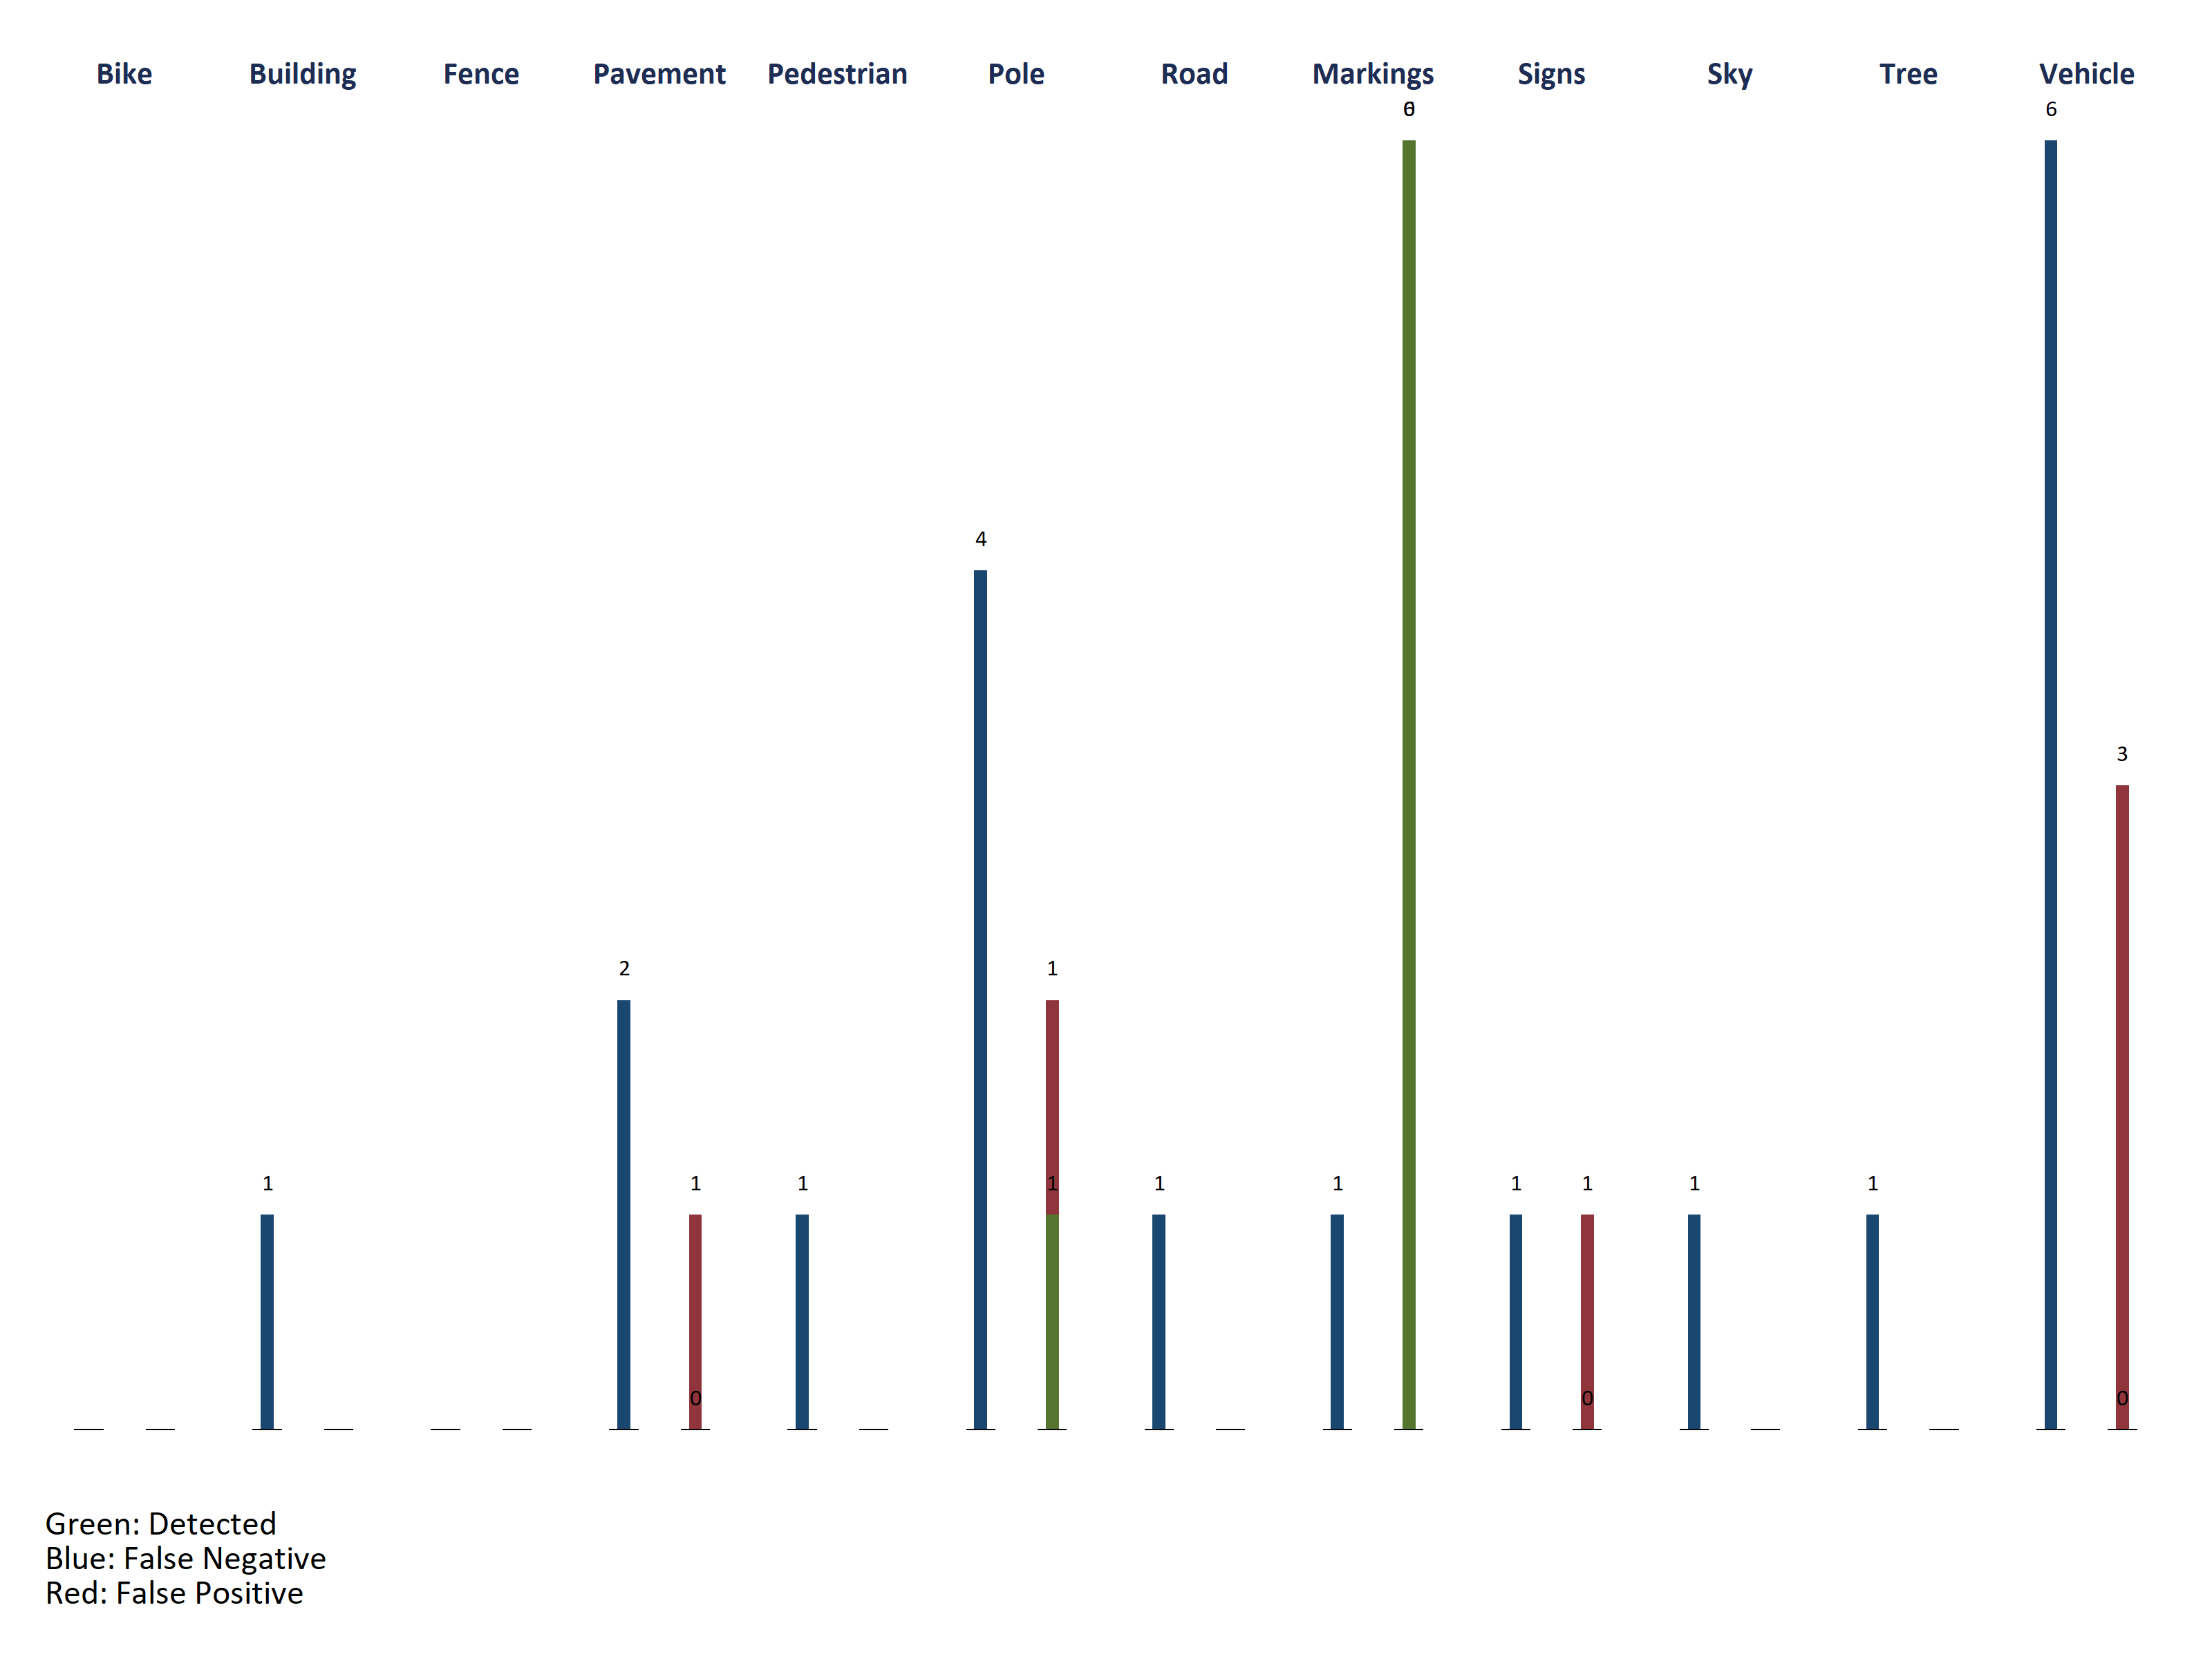
\includegraphics[width=0.9\linewidth]{figure_2}
	\caption[Detected objects and their errors]{The number of detected objects along their errors in detections according to the objects.}
	\label{fig:5:graph}
\end{figure}

The test run began with a drive through the car park. SegNet's output in Fig.~\ref{fig:5:carpark} shows that the image was segmented with good accuracy. With the exception of some minor (0.69\%)  false detections on the car's shadows on the left side, the road, parking lane, and pavements were properly segmented, along with the pedestrian and vehicles. With the LiDAR actively measuring the distance from the parked vehicles to the SAE car (see Fig.~\ref{fig:5:lidar}). Here, we adopt the Linear Regression model that we described in Section~\ref{secmethod}, which plots the road edge position from the parked vehicles so that a fixed distance can be kept between the autonomous cars and the parked vehicles. We have also counted the number of detected objects along with their positive and negative false detections, which are plotted according to their detection/error pairs in Fig.~\ref{fig:5:graph}, whereby the labelled number on each bar indicated the number of correctly identified objects, if present. 

\begin{figure}[H]
	\centering
	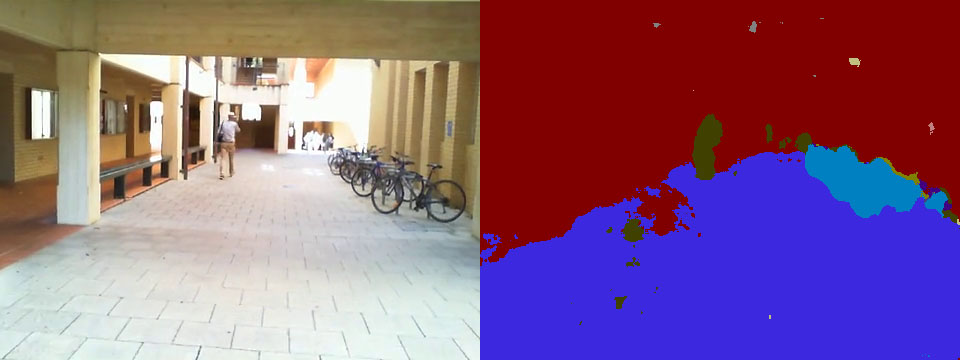
\includegraphics[width=0.8\linewidth]{3}
	\caption{Segmentation results on pavement between faculty buildings.}
	\label{fig:5:pavement}
\end{figure}

From the parking area, the car drives onto the pavement between faculty buildings. From Fig.~\ref{fig:5:pavement}, SegNet could discern pavements from roads as the grounds are now coloured blue. In addition, it was also able to detect the bicycles parked towards the right, and the pedestrians in the distance. False detections are present on the left side of the pavement, where it is incorrectly detected as buildings and pedestrians due to uneven lighting, accounting for 2.83\% of the total pavement region. 

\begin{figure}[H]
	\centering
	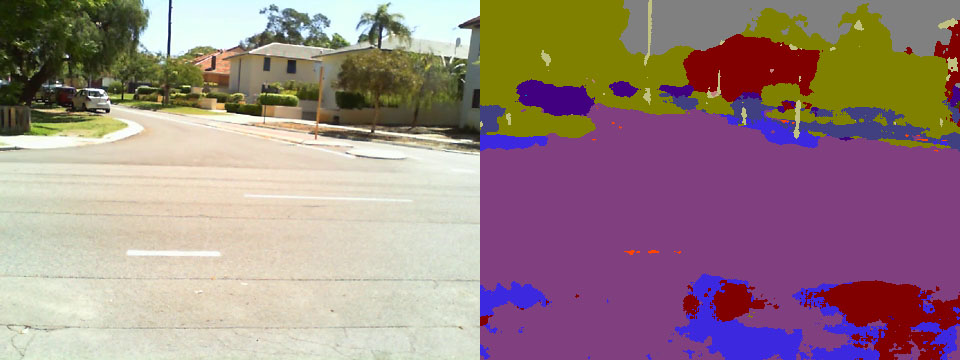
\includegraphics[width=0.8\linewidth]{4}
	\caption{Segmentation results at a road junction.}
	\label{fig:5:junction}
\end{figure}

Fig.~\ref{fig:5:junction} was captured when the car was stopping at a suburban road junction beside the campus. The segmentation output from this figure shows that while the objects in the distance were properly segmented, some parts at the bottom of the image was incorrectly classified as pavements and buildings, which makes up 16.19\% of the road region. This was partly due to the clear weather resulting in a high brightness recording, while SegNet was expecting a darker surface to classify roads. 

\begin{figure}[H]
	\centering
	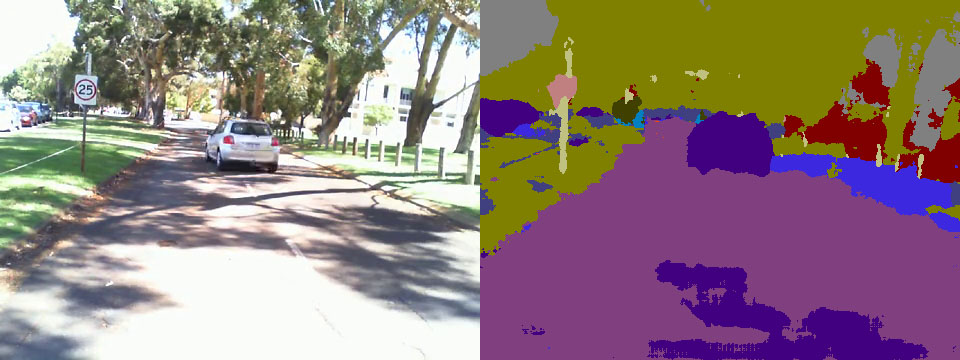
\includegraphics[width=0.8\linewidth]{5}
	\caption{Segmentation results on a road with pronounced shadows.}
	\label{fig:5:shadows}
\end{figure}

Fig.~\ref{fig:5:shadows} was captured while the car was driving on a shadowed road on campus. The shadows on the road introduced a high contrast region, and that the bottom portion of the road was overexposed, resulting in a false classification of 13.93\% and undetected lane markers. However, the overtaking vehicle, vegetation, road sign, and building were correctly segmented. When presented with a false detection on the road as with Figure~\ref{fig:5:road}, results from the LiDAR road edge detection system will compensate the regions of false detection, as the road and road edges were properly measured by the LiDAR system. 

\begin{table}[H]
	\renewcommand{\arraystretch}{1.3}
	\caption[Semantic segmentation accuracy]{The number of road region pixels and its false detections pixels in that region for each figure along with their error percentages. }
	\label{tabpixelcount}
	\centering
	\begin{tabular}{crrr}
		\toprule
		        Fig.         & Road Pixels & False Classifications &   Error \\ \midrule
		 ~\ref{fig:5:road}   &       41648 &                    16 &  0.04\% \\
		\ref{fig:5:carpark}  &       86561 &                   600 &  0.69\% \\
		\ref{fig:5:pavement} &       76731 &                  2168 &  2.83\% \\
		\ref{fig:5:junction} &      108684 &                 17595 & 16.19\% \\
		\ref{fig:5:shadows}  &       83831 &                 11679 & 13.93\% \\ \bottomrule
	\end{tabular}
\end{table}

The false detection rates for each of the example figures is summarised as Table~\ref{tabpixelcount}, which also tabulates the number of road pixels in each detected road segments for each figure, along with the number of falsely classified pixels within that road segment. From these numbers, the detection error is calculated as a percentage that corresponds to the area of each figure's road segments. The false detection rate is at its highest in Fig.~\ref{fig:5:junction}, where the road region encompasses most of the frame, the unevenness in road surface and lighting is the main contributor to this error rate. Conversely, Fig.~\ref{fig:5:road} records the lowest false detection rate its road segment, as the road area was well-defined, and the frame was properly exposed. 

\section{Conclusion}
We have presented a semantic segmentation-based visual navigation approach for autonomous ground vehicles. This approach improves on existing LiDAR-based vehicles to introduce object recognition and classification while driving. SegNet adequately performs semantic segmentation to recognise roads and lane markers, which in turn allows the vehicle to maintain a safe distance from the road and lane edges in addition to LiDAR measurements. We have also shown that the segmentation results from SegNet on the CamVid dataset is satisfactory on Perth metro roads. With a calibrated camera, visual autonomous driving can be achieved using real-time semantic segmentation. Future works will focus on the complete on-line implementation of SegNet on the SAE car for real-time visual autonomous driving.
%!TEX root = ../thesis.tex

\chapter{A Modular Software Framework for Autonomous Vehicles}
\label{ch:modular}

\ifpdf
	\graphicspath{{Chapter6/Figs/Raster/}{Chapter6/Figs/PDF/}{Chapter6/Figs/}}
\else
	\graphicspath{{Chapter6/Figs/Vector/}{Chapter6/Figs/}}
\fi

Software frameworks for autonomous vehicles are required to interface and process data from several different sensors on board the vehicle, in addition to performing navigational processes such as path planning and lane keeping. These can include a combination of cameras, LiDARs, GPS, IMU, and odometric sensors to achieve positioning and localisation for the vehicle and can be challenging to integrate. In this paper, we present a unified software framework that combines sensor and navigational processing for autonomous driving. Our framework is modular and scalable whereby the use of protocol buffers enables segregating each sensor and navigation subroutine individual classes, which can then be independently modified or tested. It is redesigned to replace the existing software on our Formula SAE vehicle, which we use for testing autonomous driving. Our testing results verify the suitability of our framework to be used for fully autonomous drives.

\section{Introduction}
UWA's Renewable Energy Vehicle Project (REV) operates two autonomous vehicles, a BMW X5 and a student-built Formula SAE-Electric car. Formula SAE~\cite{sae_international_student_nodate} is a long-running annual competition organised by the Society of Automotive Engineers with competition events worldwide. The design competition includes petrol cars, as well as the SAE-Electric class which includes ours with two electric motors driving each of the two rear wheels via independent controllers. We have incorporated full drive-by-wire control of the throttle, steering and the hydraulic braking system. The use of a Formula-SAE car provides several advantages for such a project; the car is mechanically simple, Formula-SAE cars with similar designs are common at universities worldwide and the size of the car makes testing accessible without forgoing race car vehicle dynamics. Furthermore, the use of an electric vehicle makes the project significantly more practical for student work as the risks and environmental issues associated with petrol-engine cars are eliminated and the systems installed in this project can take advantage of the large amount of electrical energy already available on the vehicle.

For the driverless FSAE project, our goal was to be able to autonomously drive a vehicle around a race track. This is being achieved by placing waypoints along the ideal driving line, as well as ``fence points" to lock out non-driving areas. Maps can either be recorded by human or remote-controlled driving or specified through a Google Maps driven web-interface. During autonomous driving, a laser scanner and camera are used for detection of road edges as well as any obstacles on the track. Safety systems are essential for a driverless system, as the car weighs more than 250 kg and is capable of driving at a speed of 80 km/h. Both the low-level drive-by-wire, as well as high-level navigation system have independent safety systems built in. These include remote intervention, remote heartbeat and remote emergency stopping, which are implemented through a fail-safe wireless link to a base station as well as through hard-wired buttons on the car itself. 

\nomenclature[z-fsae]{FSAE}{Formula SAE}

Our motivation for designing and presenting this framework is to improve upon the existing autonomous drive software on our SAE vehicle that is documented in~\cite{drage_development_2013}. This software utilises a web-based user interface (UI) that displays via a touch screen mounted in the vehicle’s cockpit. Our proposed framework utilises this existing UI with a revamped backend as described in Section~\ref{sec:6:autonomous}. It was noted that the existing software had a heavy reliance on a central Control module, which required all the sensors and their submodules to run to function. These submodules were programmed throughout the years with different programming languages and redundancies, which made integration difficult. Our proposed framework presents a streamlined approach whereby each module will be programmed with a C++ interface that communicates with either a path planner or a drive control system. This system also benefits from additional features including visualisation data playback (online or offline) and a web-based user interface. As a customised framework for our project, this also alleviates the reliance on node-based solutions such as ROS, which usually requires a perpetually running Master node to function and allows higher reliability when the individual components are integrated.

\nomenclature[z-ui]{UI}{User interface}

Additionally, this approach presents a long-term advantage whereby our framework is made fully open and contributable by students and enthusiasts looking to implement our framework onto their custom-fabricated vehicles. When compared against other autonomous driving frameworks such as Apollo~\cite{baidu_apollo_nodate} and Autoware~\cite{autoware_autoware_nodate} that mostly target commercial vehicles and requiring expensive hardware, our approach leverages on hardware and fabrication methods that are more accessible in cost.

\section{Autonomous Driving Framework}\label{sec:6:autonomous}
\begin{sidewaysfigure}
	\centering
	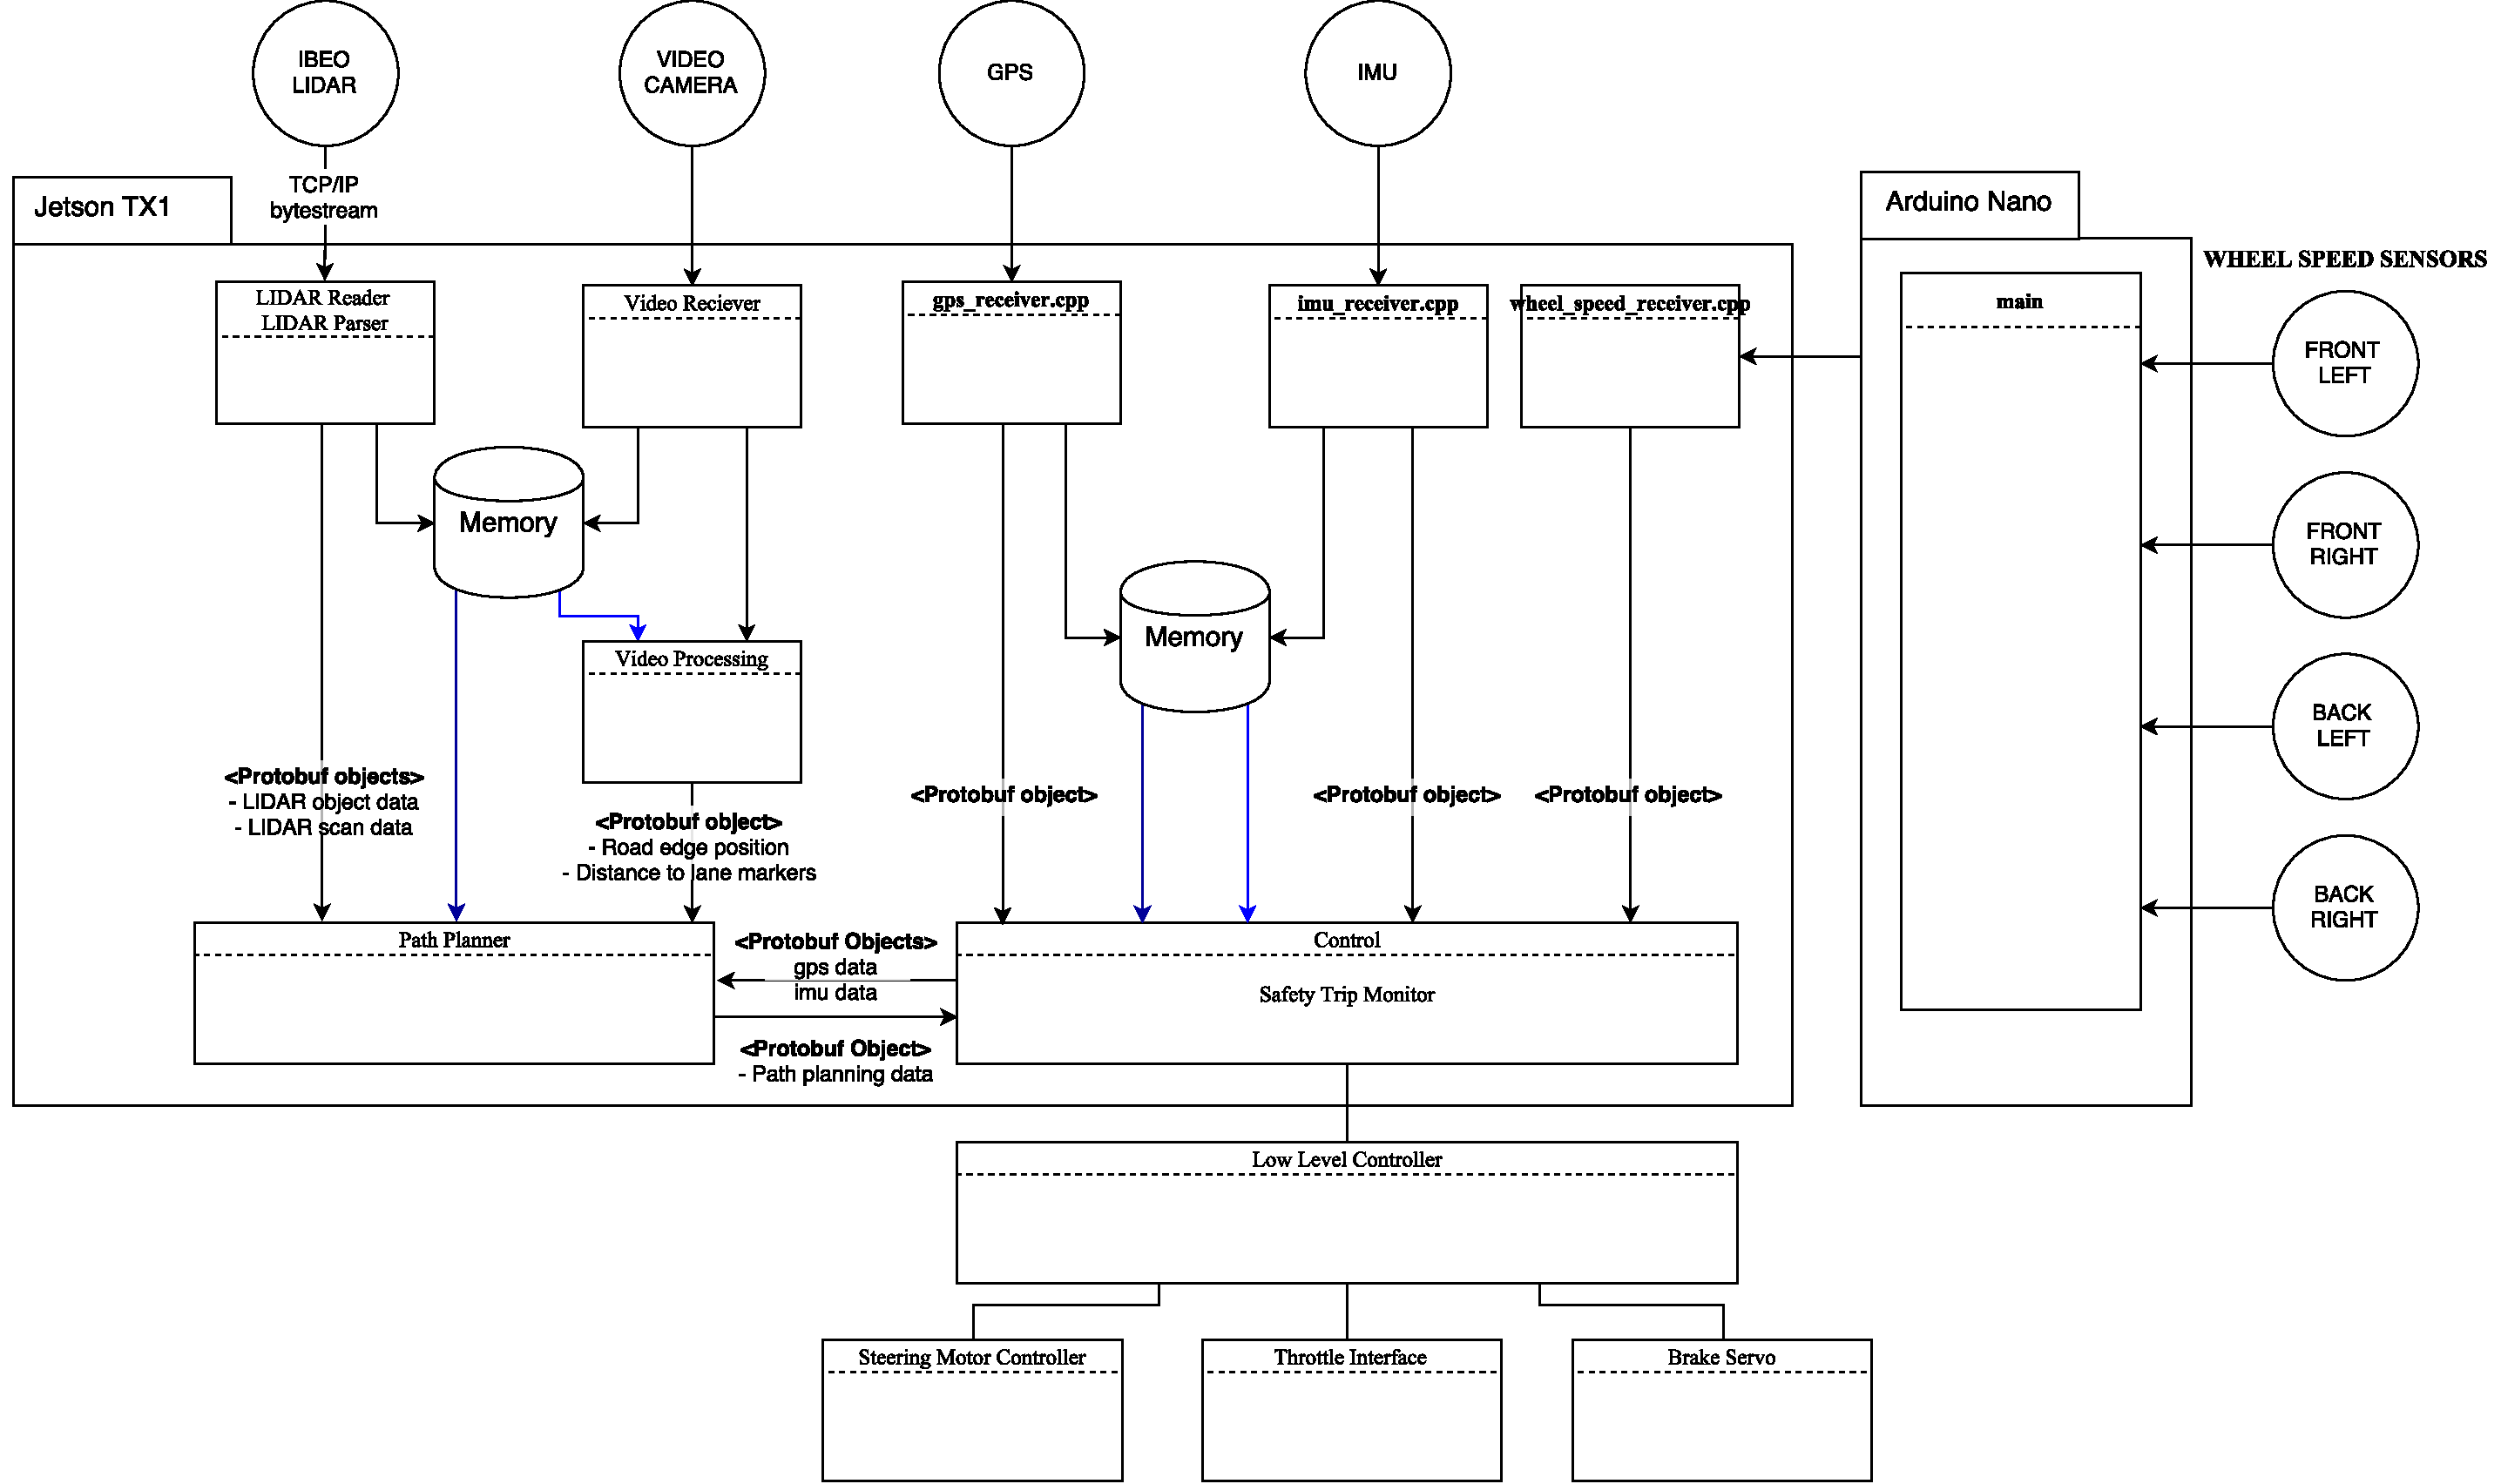
\includegraphics[width=\linewidth] {arch}
	\caption{The software architecture diagram of our proposed framework.}
	\label{fig:6:arch}
\end{sidewaysfigure}

This section introduces our proposed software framework for the SAE vehicle, with the software architecture diagram as illustrated in Fig.~\ref{fig:6:arch}. The software architecture of the vehicle utilises a modular design to allow for continuous parallel development on each of the sensors, the path planning algorithm, and the control policy. Input sensors are comprised of the LiDAR, camera, GPS, IMU and four wheel speed sensors, which are required to function simultaneously in order for the car to drive autonomously. The LiDAR, camera, GPS and IMU each have their own receiver class on the Jetson TX1, which takes the input from the sensors and processes the data. Additionally, rotary-encoder odometry is performed using an Arduino microcontroller connected to each of the wheels' encoder. This information is received in the high-level software by another receiver class which processes the data to produce wheel speed measurements. Relevant data for path planning and localisation is encoded in protobuf~\cite{google_developers_protocol_nodate} format and then passed to either the path-planning program or the control program, which performs localisation as well as some communication and logging utilities. The control program also communicates with the web GUI, providing a visualisation of the data and allows the user to start and stop autonomous driving as well as the safety trip monitor and the controller, thereby introducing a high-level interface for driving the car. The control program, once it has communicated with the path-planner to combine localisation data with a set of future way points, will transmit driving instructions to the controller. This in turn transmits them to a low-level microcontroller. Not pictured in the diagram is the fusion of data from sources such as the GPS and IMU, and IMU and LiDAR in order to improve the accuracy of localisation. Detailed explanations of the sensors and classes are covered in Sections~\ref{sec:6:pathplanner} through~\ref{sec:6:controller}.

\subsection{Path Planner}\label{sec:6:pathplanner}
We use a real-time capable path-planning algorithm based on~\cite{chu_local_2012}.
Given a set of pre-recorded or pre-defined waypoints along a track, the planner will generate a optimised path through all way points, which serves as a base frame for trajectory generation.
During operation, the algorithm evaluates a variety of possible trajectories in the configurations space of the vehicle using rapidly-exploring random trees (RRTs)~\cite{lavalle_planning_2006}.
Those intermediate trajectories are generated along a curvilinear coordinate system, along with the base frame.
Each possible trajectory is checked for collisions with obstacles. A collision free path is then picked, utilizing a cost-function, that enables us to influence the driving style of the vehicle.
The algorithms are implemented in C++14 and rely heavily on the C++ source libraries Boost and Eigen3.

\nomenclature[z-rrt]{RRT}{Rapidly-exploring random tree}

We use an arc-length parametrised cubic B-spline $P_b(s)$~\cite{wang_arc-length_2002} to generate a base frame for the curvilinear coordinate system, which can be described as a non-linear transformation of the parameter domain on the four waypoints $a$ to $d$, parametrised by $s$.
\begin{align}
	P_b(s) = \begin{cases}
	x_b(s) & = a_{x,i}(s - s_i)^3 + b_{x,i}(s - s_i)^2   + c_{x,i}(s - s_i) + d_{x,i} \\
	y_b(s) & = a_{y,i}(s - s_i)^3 + b_{y,i}(s - s_i)^2   + c_{y,i}(s - s_i) + d_{y,i} \\
	\end{cases}
\end{align}
The curvature $\kappa_b$ can be calculated from the first and second derivatives of $P_b(s)$
\begin{align}
\kappa_b = \frac{x'_by''_b - x''_by'_b}{(x'^2_b - y'^2_b)^\frac{3}{2}} &
\end{align}
where:
\begin{subequations}
	\begin{align}
	\frac{dx_b}{ds} &= x_b' = \cos\theta_b \\
	\frac{dy_b}{ds} &= y_b' = \sin\theta_b
	%\frac{d^2x_b}{ds^2} = x_b'' &\qquad \frac{d^2y_b}{ds^2} = y_b''\\
	\end{align}
\end{subequations}
The curvature of a cubic spine is continuous in all sections.
For this reason, a parametric cubic B-spline is adopted for the base frame.
Since the position of the vehicle is provided in Cartesian-space, we need to find a transform those coordinates to a curvilinear representation, of which the B-spline provides the base.
This is equal to finding the closest point to the vehicle on the base frame, by minimising the Euclidean distance between the position of the vehicle and the cubic B-spline.
\begin{equation}
\min_s d(s) = \sqrt{[x_v - x_b(s)]^2+[(y_v - y_b(s)]^2}
\end{equation}
We chose Brent's method~\cite{brent_algorithms_1973} to find the minimum. Another suitable and stable algorithm is provided in~\cite{xu_accurate_2008}.
From the lateral distance to the base frame and the base frame we construct the curvilinear coordinate system in which we generate a number $n$ of paths as cubic polynomials.
Each polynomial is defined by a lateral offset $q(s)$ and a curvature $\kappa$, to cover a broad section of the configuration space of the vehicle.
$n$ is a design parameter and can be chosen to adjust the computational load of the algorithms.
We now design a vehicle model of a set of differential equations in Cartesian space.
\begin{subequations}
	\begin{align}
	\dot{x} &= v \cos\theta \\
	\dot{y} &= v \sin\theta \\
	\dot{\theta} &= v\kappa
	\end{align}
\end{subequations}
This vehicle model is transformed onto the curvilinear coordinate system, and the position of the vehicle in Cartesian space can then be determined by forward integration.
Paths that violate the nonholonomic constraints of vehicle motions or collide with an obstacle are eliminated.
The remaining paths are evaluated by a construction. 
The cost function itself can be chosen to optimise driving for an arbitrary property, like sportiness or safety.
By simulating the path planner using equally weighted costs, the near-optimal path can be obtained as Fig.~\ref{fig:6:loop}, with the path drawn in green and the base frame in blue. The manoeuvre selection is subsequently presented as Fig.~\ref{fig:6:mano} 
Because this planner insoles a simple vehicle model as a set of ordinary differential equations, it can be conveniently integrated into any control algorithm.

\nomenclature[g-k]{$\kappa$}{Curvature}
\nomenclature[g-t]{$\theta$}{Angular orientation}
\nomenclature[a-s]{$s$}{Paramaterisation}   
\nomenclature[s-t]{$b$}{B-spline}   
\nomenclature[a-n]{$n$}{Integer set}   
\nomenclature[a-v]{$v$}{Velocity}   
\nomenclature[a-v]{$d$}{Euclidean distance}   

\begin{figure}[H]
	\centering
	\begin{subfigure}[b]{0.45\textwidth}
		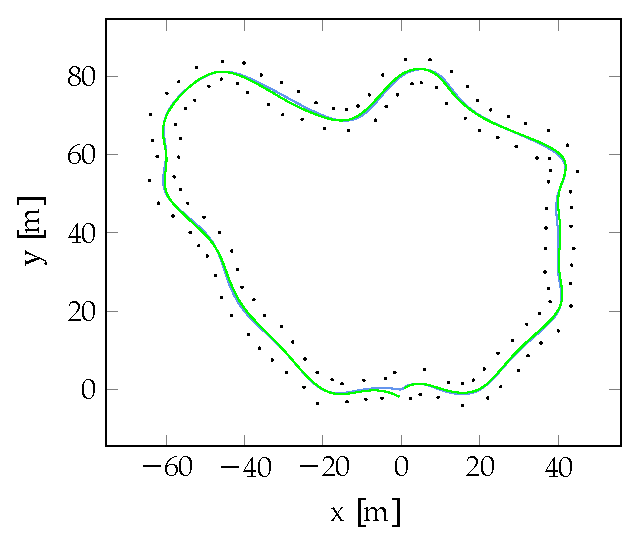
\includegraphics[width=\textwidth]{pathloop}
		\caption{Simulated path}
		\label{fig:6:loop}   
	\end{subfigure} 
	\hspace{1em}         
	\begin{subfigure}[b]{0.45\textwidth}
		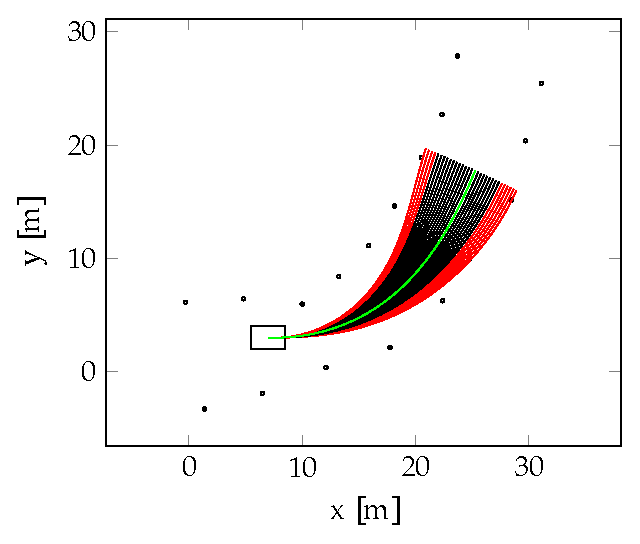
\includegraphics[width=\textwidth]{manoeuvre}
		\caption{Manoeuvre selection}
		\label{fig:6:mano}
	\end{subfigure}             
	\caption[Simulated near-optimal path and manoeuvre selection]{Simulated near-optimal path (a) and manoeuvre selection (b). Black dots represent road delimiters.}
	\label{fig:6:loopmano}
\end{figure}

\subsection{Software Communications}
The sensors on the vehicle communicate with the path planner using procotol buffers. Protocol Buffers (protobuf)~\cite{google_developers_protocol_nodate} are a formalised data structure developed by Google for use in cross-platform systems. Protobuf allows for the combination of several standard variables into a single packed structure that can be easily serialised and accessed using automatically generated methods. The protobuf library has bindings for many common programming languages, including C++, Python and Java, meaning that a protobuf structure packaged in a C++ application, can be read in by a Java application with no conversion needed. 

\nomenclature[z-protobuf]{Protobuf}{Protocol buffer}

Protocol buffers are used internally within our software as regularly structured state variables, with easy to use member functions. For example, the GPS software stores its current state within a protobuf object containing data such as latitude, longitude, ground speed and angle. This GPS state can then be used by internal code regularly, or it can be used serialised and stored.  The serialised protobuf data is very compact and space efficient, meaning that a huge amount of logged data can be saved sequentially. 

By abstracting the actual data from a specific sensor behind a protobuf object, it allows for the use of Polymorphism within our software, and so dependencies on a specific piece of hardware are loosened. As long as a specific hardware device can be interpreted into the appropriate protobuf form,  it can be integrated easily into the system, with only short wrapping code needed to be written. There is also no dependency for this protobuf data to come from a physical sensor, the protobuf data can be read in from a previously serialised log, allowing for the replay of data, or it can be read from an external piece of software, allowing for the use of simulation programs.

\subsection{Localisation}
The vehicle achieves localisation through the inertial measurement unit (IMU) and global positioning system (GPS). The IMU used in the project is the Xsens MTi~\cite{xsens_mti_nodate} 9 depth-of-field sensor. The sensor contains several advanced internal algorithms in order to provide accurate and noise-free measurements of the current gyroscopic position, the acceleration, and the magnetic field. These values are returned by the IMU readings as the velocity, acceleration, and the three rotations (pitch, roll and yaw) along the $x$, $y$ and $z$ axis. The sensor is used within the project to determine heading, and assist in the calculation of local positions. 

The GPS receiver used is the Columbus V-800 GPS receiver. It is used with the GPSd~\cite{raymond_gpsd_nodate} software to parse the National Marine Electronics Association (NMEA) standard data outputted by the GPS unit, and retransmit internally in an easier to use format. The data used from the GPS unit are the GPS coordinates, the ground speed, and the heading.  These GPS coordinates are first converted into a local reference frame, as a distance from a datum point. 
The acceleration and position data from the IMU and the GPS units respectively are fused together using an extended Kalman filter (EKF), producing a value for positioning that has a higher accuracy than GPS alone. This fusion system outputs the filtered position, velocity, and acceleration data which is then fed into the Path Planner and Control modules along with the bearing to ensure that the vehicle can reliably localise itself and obtain accurate readings for the position, velocity and acceleration. 

\nomenclature[z-nmea]{NMEA}{National Marine Electronics Association}

\subsection{Odometry}
The SAE car has been fitted with Hall Effect sensors that send its data through a comparator and an OR gate, this makes a pulse train where we use an Arduino UNO~\cite{arduino_arduino_nodate} to count the time between pulses to give angular velocity, which can be translated to meters per second. This gives the car Odometry, in which software will use an EKF to fuse the measurements together to improve their individual measurements and the vehicles’ localization capabilities. As the Arduino UNO is too slow to control the steering as well as breaking for the SAE Car, we added a second Arduino to do the odometry which then sends the data through serial communications to the main Arduino Nano. This low-level communicates steering and wheel velocity to the Nvidia Jetson TX1 for processing the data through the EKF, using a simple car kinematic model. The goal is to achieve the localization with reduced reliance on the GPS.

\subsection{LiDAR}
The Autonomous Formula SAE vehicle uses an ibeo LUX~\cite{autonomoustuff_ibeo_nodate} Light Distance and Ranging system (LiDAR) to sense distance information about the world around it. The LiDAR records the time interval between emission and recapture of thousands of infra-red light pulses to record a stream of 3-Dimensional points. The LiDAR is specifically designed for automotive purposes and is capable of internal data analysis; detecting and classifying objects in its field of vision. The LiDAR connects via an Ethernet switch to the Nvidia Jetson TX1~\cite{nvidia_corporation_embedded_2017-1}. A LiDAR reader class receives the serial bytestream which is continuously being transmitted. The data parsing is handled by the parser class which converts the bytestream into Protobuf objects. This format facilitates the storage and sharing of the information to the LiDAR visualisation.

\begin{figure}[H]
	\centering
	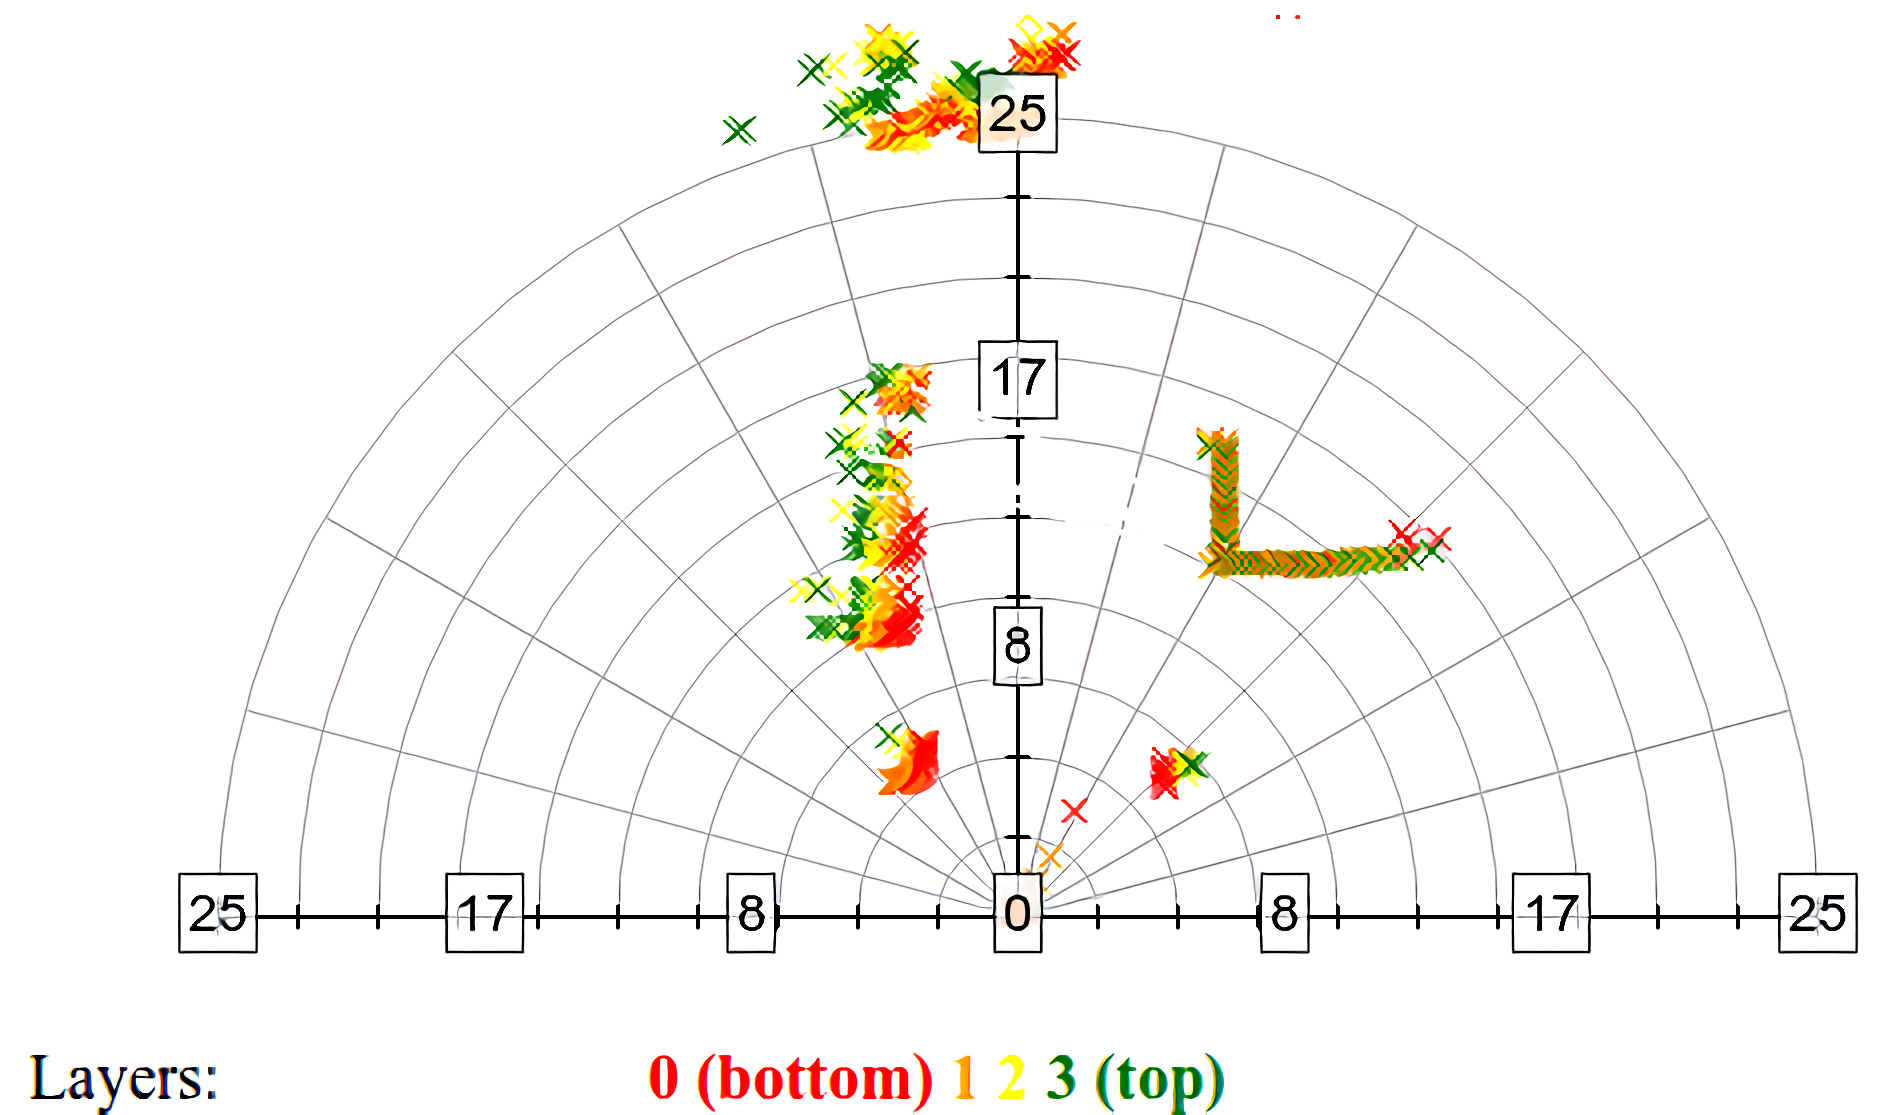
\includegraphics[width=0.8\linewidth]{luxplot}
	\caption[LiDAR plot at the position of Fig.~\ref{fig:6:carpark}]{LiDAR plot showing the detected parked vehicles at the position where Fig.~\ref{fig:6:carpark} was captured. The graph axes measure distances in metres.}
	\label{fig:6:lidar}
\end{figure}

Road-edge detection is achieved through the use of the LiDAR data. The LiDAR, aimed at an angle below horizontal beyond the front of the car, provides four layers of depth information with a horizontal angle of 85 degrees. Its output is visualised as Fig.~\ref{fig:6:lidar}. Road edge detection is achieved by analysing the depth information in one of the layers and checking it for both smoothness and slope. The central data points and those near them are considered and checked to confirm that they meet the slope criteria (the road should be relatively flat so no great changes in depth should be noted in a line) iteratively further and further points are considered in a stepwise process where the correlation coefficient is considered at each point. The road edge is the point at which the correlation coefficient is the highest whilst the slope condition is still being met. This approach was improved with the implementation of a Kalman filter which creates a time-averaged estimate of the road edge-position assisting in the prediction of the current road edge.

\subsection{Visual Navigation}
The SAE vehicle uses visual information as one of its references for driving decisions. It mainly uses an off-the-shelf monocular camera to collect images then applied through OpenCV and SegNet~\cite{badrinarayanan_segnet:_2017} for road edges detection. OpenCV provides many modules, such as image processing, video, and video input/output, that is useful for road edges detection. However, using OpenCV alone for image recognition is limited by variations in image quality, brightness, and contrast. SegNet is an image semantic segmentation approach. It can classify road scene objects, such as the pedestrian, lane marking, traffic light, vehicles etc., that complement the insufficient of single image processing scheme. SegNet is a pixel-wise semantic segmentation in deep learning framework. Semantic segmentation is used to apply for understanding the visual scene and object. This has been widely adopted in autonomous driving. The architecture of SegNet is a convolution encoder and decoder which is a pixel-wise classifier. The objects classify from SegNet is including following classes, sky, Building, column-pole, road-marking, road, pavement, tree, sign-symbol, fence, vehicle, pedestrian, and bicyclist. The accuracy of classify result is 65.9\% for classes average~\cite{badrinarayanan_segnet:_2017}. The input images utilise SegNet to perform visual scene classification. This will produce results whereby road, road-marking, and pavement are classified (see Fig.~\ref{fig:6:carpark}), which is useful for road edges detection. OpenCV is simultaneously used to perform image processing. The first step for image processing is camera calibration to get an undistorted image. This is achieved using a chess board image and finding chess board corners to get two accumulated list --- 3D point in real world space and 2D points in an image plane. Then we use the camera calibration function in the OpenCV library to obtain the camera calibration and distortion coefficients. This scheme will remove camera distortions.

\begin{figure}[H]
	\centering
	\includegraphics[width=0.8\linewidth]{2}
	\caption{Segmentation results from a parking area on campus grounds.}
	\label{fig:6:carpark}
\end{figure}

The road edges detection scheme detects lane-marking at two sides of autonomous SAE vehicle. The lane-marking detection can also be performed solely by the OpenCV library. Finding the edges of the whole image will reduce the image complexity because numbers of colour and gradient of the image would make image processing more difficult. Canny edge detection~\cite{canny_computational_1986} is a convenient approach in found in the OpenCV library that can be applied for this purpose. Then, Hough transform~\cite{hough_method_1962} can be applied onto the image to detect the lanes on both sides of autonomous SAE vehicle. The marking of lanes is detected then using perspective transforms to get a bird’s eye view-like image. It can easily find the four points to represent the lane marking pair, where a second order polynomial method can be applied to fit the points. The lane distances are obtained using pixel values that are converted into metres. The scaling factors are according to the Australian road width standard of 3.3 to 3.5 metres. However, the image processing approach might fail because the lane markings are not clear or when there are no lane markings. Therefore, using SegNet's results can effectively circumvent this drawback due to its ability to robustly detect and classify road and lane markings, whereby the same road distance calculation can be applied to find the vehicle's distances to the road edges.

\subsection{Safety Trip Monitor}
The safety trip monitor was designed with an observer-notifier structure. Any of the objects responsible for performing a safety-crucial function in the software can call a trip on the trip state monitor. This includes the low-level safety software, the controller, the GPS software, the web interface, the heart beat and the car network. The trip state is stored by the trip state monitor and pushed to any object which implements the trip state observer class and has registered itself with the monitor. The observer class ensures that the trip state does not produce any irregular operations while driving. The observers which receive the trip state upon each change are attached to the monitor after its instantiation, which means that the set of objects in the software which can change the trip state and which need to track to trip state can be completely reconfigured without needing to make changes to the trip state monitor or observer classes. This is an ideal structure for the software of a research autonomous vehicle, as the continuous development of ongoing research will frequently modify the structure of functions of portions of the software while seeking to maintain the integrity of safety features, like the safety trip.

\subsection{Controller} \label{sec:6:controller}
The controller class is the high-level interface for the drive-by-wire functionality of the vehicle. The actual drive-by-wire controlling of the vehicle is done by separate software on an Arduino microcontroller. The controller class is the only high-level software which communicates with the low-level controller. The program utilizes three PID controllers to set the throttle, brake, and steering values. The controller class provides a high-level interface with methods to begin to stop autonomous control of the throttle, brake, and steering, as well as methods to set the bearing or speed of the vehicle with desired values. This interface is utilized by the Control program, which handles path planning, and the Fusion program, which provides fused IMU-GPS data in order to facilitate waypoint-based driving. Fig.~\ref{fig:6:base frame} and~\ref{fig:6:curvature} illustrates the base frame and curvature output by the path planner using the Control program based on our evaluation path in Section~\ref{sec:6:implement}. A large change in curvature is present where the U-turn was made.

\nomenclature[z-pid]{PID}{Proportional--integral--derivative (controller)}

\begin{figure}[H]
	\centering
	\begin{subfigure}[b]{0.45\textwidth}
		\def\svgwidth{\textwidth}
		\input{Chapter6/Figs/PDF/baseframe.pdf_tex}
		\caption{Baseframe trajectory}
		\label{fig:6:base frame}   
	\end{subfigure} 
	\hspace{1em}         
	\begin{subfigure}[b]{0.45\textwidth}
		\def\svgwidth{\textwidth}
		\input{Chapter6/Figs/PDF/curvature.pdf_tex}
		\caption{Derived curvature}
		\label{fig:6:curvature}
	\end{subfigure}             
	\caption[Generated trajectory base frame]{The trajectory base frame generated by the path planner (a) and its derived curvature (b).}
	\label{fig:6:basecurve}
\end{figure}

\section{Implementation on SAE Vehicle} \label{sec:6:implement}
The software for the autonomous driving system is programmed onto an Nvidia Jetson TX1  embedded computer that is mounted on the chassis of the vehicle. The environmental sensors namely the LiDAR, GPS, IMU and camera connects directly to the camera via Ethernet (LiDAR) and USB 2.0 (GPS, IMU, camera) respectively. This software can be implemented onto another vehicle so long as the same sensors are used, as the system outputs drive commands through the Control module, which can be configured according to the vehicle's hardware specifications. To test our system, we collected driving data with the vehicle driving in a parking area at the University of Western Australia (shown in Fig.~\ref{fig:6:map}) by recording readings from the GPU, IMU, LiDAR and camera. The GPS and IMU plots waypoints for the car, LiDAR performs obstacle detection, and the camera performs semantic segmentation. The test drive begins from the southern end and then driving towards the northern end before making a U-turn back to the vehicle's station position. The recorded waypoints are passed to the path planner, which generates a trajectory base frame as shown in Fig.~\ref{fig:6:base frame}. Subsequently, the curvature is obtained from the derivative of the base frame as Fig.~\ref{fig:6:curvature}, which can then be used to determine the steering angle for autonomous driving. 

\begin{figure}[H]
	\centering
	\def\svgwidth{0.7\linewidth}
	\input{Chapter6/Figs/PDF/map.pdf_tex}
	\caption{Map showing the path taken by the vehicle in with a solid red line.}
	\label{fig:6:map}
\end{figure}

\section{Results}
Fig.~\ref{fig:6:carpark} was captured while the car was driving northward as it approaches the end of its path. The input image is displayed on the left and its semantic segmentation result is displayed on the right image. Results from semantic segmentation showed that the road is properly classified, along other elements in the frame. Its LiDAR readings at that position is as illustrated in Fig.~\ref{fig:6:lidar}, whereby the parked vehicles are detected on the left, along with the vegetation in the distance and the wall on the right side of the vehicle. The combination of LiDAR and semantic segmentation enables the vehicle to understand its position on the road, along with the obstacle types and the distances to each obstacle. For further results on road and lane marker detection, we processed a drive recording from Udacity's Self-Driving Car Nanodegree~\cite{udacity_self-driving_2017}. From Fig.~\ref{fig:6:segnetroad}, the input image (Origin) is used for both semantic segmentation (SegNet), and bird's eye view transformation (Bird view). The system was able to identify objects on the road scene, and the curvature of the road can be calculated using the bird's eye view. The distance between the centre of the vehicle and the left and right lane markers are calculated as shown in the output. This is accompanied with a confidence value whereby a successful detection of the road lane markings will be denoted with a ``1''.  

\begin{figure}[H]
	\centering
	\includegraphics[width=0.8\linewidth]{segnet_road}
	\caption[Visual navigation output]{Original and Jetson TX1 output showing segmentation, bird’s eye view, vehicle distance to left and right lane marks.}
	\label{fig:6:segnetroad}
\end{figure}

\section{Conclusion}
In this paper, we have designed and demonstrated the functionality of our software framework that is implemented on our autonomous SAE vehicle. This framework is designed to cohesively interface with the vehicle's camera, LiDAR, GPS, IMU and wheel speed sensors while being capable of performing navigational tasks such as path planning, image processing, odometry, localisation, safety checks, speed and steering control. Each sensor and navigation task is programmed as a separate module to ensure modularity and scalability, allowing for each module to be changed independently. Protocol buffers handle intermodular communications, whereby each process parses its output as a protobuf to be sent to another module. With this framework implemented on the Jetson TX1, our test drives on the autonomous SAE vehicle was able to achieve results that are adequate for fully autonomous driving. Future works will include further testing of the autonomous navigation software and refinements to the control and path planner classes to ensure that the system is capable for road drives using full automation. 
%!TEX root = ../thesis.tex

\chapter[Evolution of a Reliable and Extensible High-Level Control System]{Evolution of a Reliable and Extensible High-Level Control System for an Autonomous Car}
\label{ch:evo}

\ifpdf
	\graphicspath{{Chapter7/Figs/Raster/}{Chapter7/Figs/PDF/}{Chapter7/Figs/}}
\else
	\graphicspath{{Chapter7/Figs/Vector/}{Chapter7/Figs/}}
\fi

The reliability of autonomous vehicles is heavily dependent on their software frameworks, which are required to interface and process data from many different sensors on board the vehicle, perform navigational processes such as path planning and lane keeping, take action to ensure safety and display data to an operator in a useful fashion. These sensors can include a combination of cameras, LiDARs, GPS, IMU, and odometric sensors to achieve positioning and localisation for the vehicle and nearby objects in their environment and can be challenging to integrate. In this paper, we present a hybridised software framework that combines sensor and navigational processing for autonomous driving. Our framework utilises a modular approach for interfacing and safety functionality, whilst navigation and sensor interfaces are implemented as nodes in the Robot Operating System (ROS). Our testing results verify the suitability of our framework by integration with a hardware-in-the-loop simulation system and for fully autonomous field driving.

\section{Introduction}
The Renewable Energy Vehicle Project (REV) at UWA has developed an intelligent autonomous test vehicle, utilising a Formula-SAE race car (see Fig.~\ref{fig:7:car}) as a platform (Formula SAE~\cite{sae_international_student_nodate} is an annual student competition organised by the Society of Automotive Engineers with events worldwide). Using such a vehicle allows us to target driving applications, both on- and off-road, in structured and unstructured driving environments. We have incorporated full drive-by-wire control of the electric vehicle's throttle, steering and the hydraulic braking system. The use of a Formula-SAE car provides several advantages for such a project as the vehicle is mechanically simple. Formula-SAE cars with similar designs are common at universities worldwide and the size of the vehicle makes testing accessible. Furthermore, the use of an electric vehicle makes the project significantly more practical for student work and the hardware installed in this project can take advantage of the large amount of electrical energy already available on the vehicle.

\begin{figure}[H]
	\centering
	\includegraphics[width=0.7\linewidth]{car}
	\caption{Autonomous SAE Vehicle.}
	\label{fig:7:car}
\end{figure}

For the driverless FSAE project, our goal was to be able to autonomously drive a vehicle around a race track. Initially, this was achieved by placing waypoints along the ideal driving line, as well as ``fence points" to lock out non-driving areas. Maps can either be recorded by human or remote-controlled driving or specified through a Google Maps driven web interface. During autonomous driving, a laser scanner and camera are used for detection of road edges as well as any obstacles on the track. Our current work involves increasing the level of automation to drive a semi-structured (traffic cone or road edge delineated) race track by first automatically driving and mapping the path without prior knowledge of the track and then redriving it, optimised, at greater speed with the assistance of inertial navigation.

Safety systems are essential for a driverless system, as the car weighs more than 250 kg and is capable of driving at a speed of 80 km/h. Both the low-level drive-by-wire, as well as high-level navigation system have independent safety systems built in. These include active geofencing, remote intervention, remote heartbeat and remote emergency stopping, which are implemented through a fail-safe wireless link to a base station as well as through hard-wired buttons on the vehicle itself. 

The previous revision of our framework~\cite{drage_development_2013, lim_modular_2018} had a heavy reliance on a central control module, which required all the sensors and their submodules to function. These submodules were developed over time using different programming languages and are partially redundant, which made integration difficult. First, this was streamlined in an approach whereby each module is programmed with a C++ interface that communicates with either a path planner or a drive control system. Here, we present the integration of this approach with the Robot Operating System~\cite{open_source_robotics_foundation_ros/introduction_nodate} which allows the further separation of functions into ROS nodes and provides a consistent application programming interface (API) for implementation of additional sensors and higher level automation, whilst the original program, now running as a ROS node, deals with critical interfacing and safety functions.

\nomenclature[z-api]{API}{Application programming interface}

Additionally, this approach presents a long-term advantage whereby our framework is made fully open and contributable by students and enthusiasts looking to implement our framework onto their custom-built vehicles. When compared against other autonomous driving frameworks such as Apollo~\cite{baidu_apollo_nodate} and Autoware~\cite{autoware_autoware_nodate} that mostly target commercial vehicles requiring expensive hardware, our approach leverages hardware and fabrication methods that are more affordable. The framework has been integrated with a simulator which provides the ability to test software modifications and algorithms prior to deployment to the vehicle.

Our contributions in this paper are demonstrated through the proposal of our high-level autonomous control system that interfaces through standard, off-the-shelf sensors and equipment. This system is made holistic through the integration of the following features --- real-time localisation through odometry and dead-reckoning; object segmentation and detection using LiDAR and camera; real-time path planning via waypoints or object positioning; visual navigation with odometry, object recognition and tracking, and semantic segmentation; and a hardware-in-the-loop simulator for prototyping verification.  

The remainder of this paper is organised as follows. Section~\ref{sec:7:overview} introduces the system framework with an overview. Section~\ref{sec:7:sensors} describes the sensors that are used. Section~\ref{sec:7:path} presents the path planning approaches used in the system. Section~\ref{sec:7:vision} explains how visual navigation is performed on the system. Section~\ref{sec:7:sim} highlights our driving simulator. Section~\ref{sec:7:bench} describe our system validations, before the concluding remarks are drawn in Section~\ref{sec:7:conclusion}.

\section{System Overview}\label{sec:7:overview}
In order to satisfy the requirements of resiliency, flexibility, extensibility and simple integrations, a publish/subscribe software architecture was used. This allowed for highly decoupled software to be developed, with each component or series of components needing only to conform to the expected message type on the input and output topics.  The use of a publish/subscribe architecture allows for nodes to be easily swapped in and out in order to test different solutions, as well as allowing multiple components to make use of the same data sources without modifying the source, providing simple methods of logging, data capture and data replay.

It was decided to use ROS as the publish/subscribe layer of the application. This decision was influenced heavily by the usage of ROS in the Apollo Auto~\cite{baidu_apollo_nodate} project, as it is shown to be reliable and performant. This also provides a path for upgrades, with a version of ROS modified for automotive use through the addition of shared memory transport for message passing, support for the Protobuf~\cite{google_developers_protocol_nodate} message passing protocol, and the decentralisation of ROS to reduce single points of failure available on an open-source licence. This also allows for any components developed to be more easily ported to the complete Apollo Auto platform at a later stage. In addition, the popularity of ROS ensures that there are a large number of existing modules available for use, allowing the team to focus on the goals stated above, instead of on creating supporting code and utilities.
Based on the desired functionality, it was determined that the publish/subscribe architecture would initially require the nodes and topics outline in Fig.~\ref{fig:7:architecture}.

\begin{figure}[H]
	\centering
	\includegraphics[width=0.8\linewidth]{rosnodes}
	\caption{SAE vehicle software framework.}
	\label{fig:7:architecture}
\end{figure}

We migrated the existing code base of the high-level software system to use the ROS framework in 2018 to reduce the development complexity of the software system. ROS provides low-level device control, implementation of commonly used tools, message passing between processes, and package management~\cite{open_source_robotics_foundation_ros/introduction_nodate}. Instead of creating an independent system where a \textit{broker} would manage the intercommunications between \textit{modules} (programs that have a specific function) ROS readily provides these services. Hence, the user only has to create \textit{nodes} (programs that perform a certain function) that listen and talk to other nodes. Using ROS therefore simplifies the integration process for each individual module in the system. By defining the topic information for messages to communicate, the individual nodes can work together without too much effort in integration. 

More specifically, existing modules in our system presented in~\cite{lim_modular_2018}, including modules for logging, web server and serial communication were replaced with their equivalent ROS packages, as they are often more stable and better supported. All existing messages from the system are converted into ROS messages. The testing for the individual modules therefore only requires minimal changes to the core software.

The ROS version used on the SAE vehicle is currently ROS Kinetic Kame running on Ubuntu 16.04 LTS which will be long-term supported until April 2021.

\section{Navigation Sensors}\label{sec:7:sensors}

\begin{figure}[H]
	\centering
	\includegraphics[width=0.45\linewidth]{sensorrack}
	\caption{The SAE vehicle's rack-mounted sensors.}
	\label{fig:7:rack}
\end{figure}

The SAE vehicle performs autonomous driving through a combination of navigation sensors including LiDARs, cameras, wheel odometry and inertial measurement unit (IMU) (as shown in Fig.~\ref{fig:7:car}, with the sensor rack detailed in Fig.~\ref{fig:7:rack}) which are categorised into four categories --- odometry, dead reckoning, LiDAR and camera systems, which are elaborated upon in their individual Sections~\ref{sec:7:odometry} to~\ref{sec:7:camera}.

\subsection{Odometry}\label{sec:7:odometry}
The SAE vehicle has been fitted with Hall Effect sensors on each wheel which send data through a comparator and an \texttt{OR} gate, and generate a pulse train to an Arduino Nano~\cite{arduino_arduino_nodate-1}. The sensors count pulses for each wheel and report them to the low-level controller with timestamps. The linear velocity and rotational velocity are then evaluated by a low-level controller with the feedback from the steering sensor. The accumulated pose information is then combined with the wheel odometry of the SAE car. The goal for implementing this wheel odometry is to provide basic offline localisation within a low-level system and to be further fused with other sensors such as IMU, LiDAR and cameras for a more accurate global positioning.

\subsection{Dead Reckoning}\label{sec:7:dr}
Having an accurate state estimation is crucial for making optimal decisions for future control inputs to effectively navigate the environment. Dead reckoning on the vehicle is achieved through the Xsens MTi-G-710~\cite{xsens_mti-g-710_nodate}, which is an inertial measurement unit (IMU) that is equipped with a global navigation satellite system (GNSS) running at 50 Hz. However, these sensors are susceptible to noise and imperfections which introduce uncertainty to the measurements. Hence, we introduce an extended Kalman filter (EKF) to fuse data from these sensors with that from odometry using a model of the car's dynamics to obtain a more precise estimate of its state. Since the computation of the car's movements requires direction, trigonometric functions are needed. The EKF linearises these non-linear functions using a first-order Taylor series approximation~\cite{yu_derivation_nodate}, where it is approximated according to~\cite{morrell_extended_1997} in equation (\ref{eqn:f_uk}). 
\begin{align}\label{eqn:f_uk}
f(u_k,x_{k-1}) \approx f(u_k, x_{k-1}) + \frac{df(u_k, \mu_{k-1})}{dx_{k-1}}(x_{k-1} - \mu_{k-1})
\end{align}
where $u$ and $\mu$ are the mean and the estimate of $x$, respectively. With an EKF, we calculate the fused covariance values $P_k$ by predicting next state and the next error covariance using the current state and current estimate error covariance. $x_k$ is the current pose at time instance $k$ and $f$ is a non-linear transition function that converts the past state to the current state; state $x$ is composed of the car's $x$-$y$ coordinates and orientation $\varphi$. We perform this as a three-step process, following the descriptions in Section III of~\cite{moore_generalized_2016}:
\begin{enumerate}
	\item Compute the Kalman gain $K$
	\item Perform the correction to find the current state $x_k$, and
	\item Calculate the new process error $P_k$
\end{enumerate}
This is used as the foundation for our experiments on sensor fusion, as described in Section~\ref{sec:7:sensorfusion}.

\nomenclature[g-u]{$\mu$}{Estimate of $x$ [Chapter~\ref{ch:evo}]}
\nomenclature[a-u]{$u$}{Mean} 
\nomenclature[a-k]{$K$}{Kalman gain} 
\nomenclature[g-phi]{$\varphi$}{Vehicular orientation} 

\subsection{LiDAR System}
The vehicle utilises an array of Light Distance and Ranging (LiDAR) systems. This consists of a SICK LMS111-1010~\cite{sick_ag_lms111-10100_nodate} and an ibeo LUX 4~\cite{autonomoustuff_ibeo_nodate} connected through an Ethernet switch to the Nvidia Jetson TX1. The LMS111 scans a single layer at 50 Hz while the LUX scans four layers at 10 Hz featuring in-built object detection and tracking. 
The data is published by each of the LiDAR's ROS drivers and processed to achieve desired functionalities.

The LMS111 is mounted forward-facing on the front of the vehicle at 15 cm above the ground to obtain a \ang{270} field of view, suitable for detecting close obstacles and scans a plane close to horizontal. The point cloud is sorted and then from left to right; each point is assigned a cluster identification number based on distance to the next point and the angle between it and the next point relative to the laser. This delivers accurate obstacle detection with features such as cluster size indicating the size of the obstacle, allowing for classification of obstacles (such as a cone). The LUX is mounted above the driver and pitched towards the ground slightly such that the lower layer scans the ground 20 metres ahead of the vehicle. It is utilised to achieve road edge and object detection at a distance. 

Road edge detection is achieved by analysing the depth information in one of the layers and checking it for both smoothness and slope. The central data points and those near them are considered and checked to confirm that they meet the slope criteria (the road should be relatively flat so no great changes in depth should be noted in a line). Iteratively, further and further points are considered in a stepwise process where the correlation coefficient is considered at each point. The road edge is the point at which the correlation coefficient is the highest whilst the slope condition is still being met. This approach was improved with the implementation of a Kalman filter which creates a time-averaged estimate of the road edge-position assisting in the prediction of the current road edge. A detailed description of our methods is presented in~\cite{drage_lidar_2015}.

\begin{figure}[H]
	\centering
	\includegraphics[width=0.8\linewidth]{pointcloud}
	\caption[Captured scene with its instantaneous LiDAR point cloud]{Point cloud generated from the LMS111 (coloured) and the LUX (4-layers, white) (left) and the scene where it was captured (right).}
	\label{fig:7:pointcloud}
\end{figure}

The in-built object detection and tracking of the LUX will be used for fusion with the obstacles reported through processing of the LMS111's data. The comparison of positions of objects reported by the LUX and LMS111 will increase the likelihood of detecting an object. The LMS111 giving information on the objects on a low and horizontal plane and the LUX giving information of objects in the mid to far range. In turn, this object information will also be fused with that of the camera vision. 
We use both LiDARs to collectively generate a point cloud as illustrated in Fig.~\ref{fig:7:pointcloud}, captured during a test run. 
The LMS111 point cloud is coloured based on its intensity, retrieving information on the reflectivity of the surface struck by each point. The LUX is scanning layers onto the path in the distance while also picking up a large amount of detail from the surrounding vegetation as pedestrians walk past.

\subsection{Camera System}\label{sec:7:camera}
A pair of FLIR Blackfly GigE~\cite{flir_blackfly_nodate} cameras are mounted on the vehicle's frame to perform tasks related to visual navigation, such as semantic segmentation and visual odometry. These cameras are fitted with Fujinon f/1.2, 2.8--8 mm wide-aperture varifocal lenses~\cite{flir_fujinon_nodate}, and are individually capable of capturing a wide field of view. To suit our application, these cameras use 1.3 megapixel 1/3" global shutter CCD image sensors that will not be affected by any distortions caused by the rolling shutter effect~\cite{liang_analysis_2008}. The cameras are connected to a Gigabit Ethernet switch that connects to the Jetson TX1, interfacing them through Blackfly's ROS node where it is configured to record at 10 Hz per channel.

\nomenclature[z-ccd]{CCD}{Charge-coupled device}

At the time of writing, the use of stereoscopic vision for autonomous driving is still subject to evaluation. Our application focuses on using monocular vision that is paired with measurements from the LiDAR system in order to achieve depth perceptions. The methods that we use for semantic segmentation and visual odometry for this paper currently do not require a stereoscopic setup. Our implementation of these methods is further described in Section~\ref{sec:7:vision}.

\section{Path Planning}\label{sec:7:path}
We have programmed the control system to deliver path planning routines to drive either through a series of predefined waypoints, or in between a series of traffic cones placed on either side of the vehicle.

\subsection{Waypoint Driving}\label{sec:7:waypoint}
The underlying idea behind waypoint driving is to drive a set of predefined points in between the starting position $P_1$ ($x$ = 0, $y$ = 0 and orientation $\varphi$ = 0) to the destination position $P_2$, which can be obtained through the differences in GPS coordinates. These waypoints can either be stored in Cartesian coordinates in an array or in our test case, they are selected based on the driver's preference by selecting position points on RViz~\cite{kam_rviz:_2015}, which are then confirmed on the console. To ensure that all points can be driven smoothly with the consideration of the correct heading to the subsequent point, a spline approach has been implemented within this design to generate the desired path.

Once the waypoints are chosen, two static paths are shown on RViz (see Fig.~\ref{fig:7:waypoint}). The first path (green) consist of straight lines that interlink all the points with the arrow at the end showing the destination heading. The second path (purple) is the desired path which consists of a smoothed curvature that passes through all of the waypoints, the generation of this path is based on the Hermite spline interpolation technique~\cite{de_boor_practical_1978} with the required parameters which are the four vectors:
\begin{enumerate}
    \item Current position, $P_1$
    \item Target position, $P_2$
    \item Tangent of departure from current position, $T_1$
    \item Tangent of approach from target position, $T_2$
\end{enumerate}
Along with four Hermite basis functions $H_n(u)$
\begin{subequations}
	\label{eqn:hermitebasis}
	\begin{align}
	H_1(u) &= 2u^3-3u^2+1 \\
	H_2(u) &= -2u^3+3u^2 \\
	H_3(u) &= u^3-2u^2+u \\
	H_4(u) &= u^3-u^2
	\end{align}
\end{subequations}
where $0 \leq u \leq 1$ which represents the start to finish motion. We then construct the resultant path $f$ by calculating the product between the vectors and the Hermite basis functions
\begin{align}\label{eqn:hermite}
f(x,y,\varphi) = H_1P_1 + H_2P_2 + H_3P_3 + H_4P_4
\end{align}

\nomenclature[a-H]{$H_n$}{Hermite basis function} 
\nomenclature[a-P]{$P_x$}{Position at $x$} 

\begin{figure}[H]
	\centering
	\includegraphics[width=0.6\linewidth]{waypoint}
	\caption{Calculated waypoints on RViz with inputs from~\eqref{eqn:hermitebasis} and~\eqref{eqn:hermite}.}
	\label{fig:7:waypoint}
\end{figure}

The actual simulated driving pattern (red line) is determined based on the distance measurement between the current position of the vehicle against the desired path (purple) with a predefined tolerance range, and limited maximum turning angle ranged between $\pm\ang{25}$. The desired path is constituted by a finite number of points generated from the Hermite spline interpolation. To avoid oversteering or understeering, we compute the slope differences for both the driving path and the desired path.  With this logic in place, the vehicle is either turning left ($\varphi$ \textgreater\ \ang{0}), right ($\varphi$ \textless\ \ang{0}) or moving straight either at a constant speed or slowed speed for a sharper turn in order to reach the goal point ($\varphi$ =\ \ang{0}).

\subsection{Cone Driving}\label{sec:7:cone}
The current iteration of the path planning procedure uses obstacle detection of the cones to determine the correct path. This algorithm is similar to our solution in~\cite{lim_modular_2018}, but simplified to allow for quicker calculation. Our cone driving module accepts cone locations from either the map, LiDAR or camera, classifying them as objects. Then, the vehicle navigates to drive within the track formed by cones safely without collision. Using a range of the maximum turning circle of the car, of both a left-hand turn and right-hand turn, it then looks at which predicted paths will intercept cones. The vehicle dynamics are thus limited during motion planning such that the steering angle does not exceed \ang{25}. Our algorithm will iterate through all cones within the car's range and calculate the best collision-free path to undertake, as detailed in Algorithm~\ref{algo:7:cones}.

\begin{algorithm}
	\begin{flushleft}
		\caption{Cone driving}\label{algo:7:cones}
		\begin{algorithmic}[1]
			\Procedure{ConeDrive}{cones in range}
			\State init \textit{steering\_range} to [-25,25]
			\For{all \textit{cones} in \textit{range}}
			\State evaluate \textit{collision\_range} with \textit{cone}
			\State exclude the \textit{collision\_range} from \textit{steering\_range}
			\EndFor
			\If{\textit{steering\_range} is empty}
			\State stop
			\ElsIf{all \textit{steering\_range} $\leq$ \textit{threshold}}
			\State select largest \textit{steering\_range}
			\ElsIf{all \textit{steering\_range} $>$ \textit{threshold}}
			\State select \textit{steering\_angle} with minimum change in current direction
			\EndIf
			\State drive toward centre of \textit{steering\_range}
			\EndProcedure
		\end{algorithmic}
	\end{flushleft}
\end{algorithm}

\section{Visual Navigation}\label{sec:7:vision}
The vehicle is capable of performing visual navigation tasks through a combination of semantic segmentation, visual odometry and visual cone detection that is decided depending on the application requirements. These tasks commonly rely on the OpenCV~\cite{opencv_opencv_2016} library, utilising functions such as handcrafted feature detection, general image processing and transforming. It achieves a visual perception of the driving environment through the camera system as described in Section~\ref{sec:7:camera}.

\subsection{Road and Lane Detection}\label{semseg}
Our system uses either semantic segmentation or edge detection to detect road edges and lane markings, depending on the environment's complexity. Using semantic segmentation also enables obstacle recognition which can be integrated with the LiDAR system. Environments are complex when there is a lack of uniformity in pose, features and illumination. While it is possible to solely rely on modules within OpenCV here, the performance of using handcrafted features alone for image recognition is restricted by variations in image quality, brightness, and contrast. In order to improve its performance under these environments, we selected SegNet~\cite{badrinarayanan_segnet:_2017} for semantic segmentation due to its high compatibility and ease of implementation. Its ability to perform pixel-wise classification for road scene objects complements the drawbacks of a single image processing scheme.

The architecture of SegNet uses a convolution encoder and decoder setup that classifies objects into one of the following classes --- sky, building, column-pole, road-marking, road, pavement, tree, sign-symbol, fence, vehicle, pedestrian and bicyclist; with a class average classification accuracy of 65.9\%~\cite{badrinarayanan_segnet:_2017}. Our application uses SegNet whereby road, road markings, and pavement are classified (see Fig.~\ref{fig:7:segnet}), which is useful for road edges detection. However, OpenCV is simultaneously used to perform image processing, with the first step being camera calibration to get an undistorted image. This is achieved using a chessboard image and finding its corners to get two accumulated list --- a 3D point in real-world space and a 2D point in an image plane. We then use the camera calibration function in the OpenCV library to obtain the camera calibration and distortion coefficients. Our experiments using SegNet for autonomous driving was performed in~\cite{k._l._lim_implementation_2017}, where we have evaluated its segmentation accuracy in our test environment through the calculation of its pixel accuracy (PA).
\begin{align}\label{eqn:PA}
\textrm{PA} = \frac{\sum_{i}n_{ii}}{\sum_{i}t_i}
\end{align}
where $n_{ii}$ represents the number of classified class $i$ pixels correctly classified to belong in class $i$, and $t_i$ represents the total number of pixels in class $i$ belonging in the ground truth.

\nomenclature[s-i]{$i$}{Classified class (semantic segmentation)}   

\begin{figure}[H]
	\centering
	\includegraphics[width=0.8\linewidth]{segnet}
	\caption[Semantic segmentation results from test drive]{Semantic segmentation results during a test drive. This scene resulted in a pixel accuracy of 99.31\%.}
	\label{fig:7:segnet}
\end{figure}

The road edges detection process finds lane markings at both sides of the car. We have noted that lane marking detection can also be performed solely using OpenCV functions, especially in non-complex, uniform environments with minimal illumination variations, thereby reducing its computation requirements. Algorithm~\ref{algo:7:lanes} describes our approach.

\begin{algorithm}
	\begin{flushleft}
		\caption{Road and Lane Detection}\label{algo:7:lanes}
		\begin{algorithmic}[1]
			\Procedure{LaneDetect}{\textit{histogram\_vector} from camera}
			\State undistort \textit{image\_frame} from lens distortions
			\State Sobel filter \textit{image\_frame} as \textit{filtered\_image}
			\State threshold \textit{filtered\_image} as \textit{binary\_image}
			\State obtain \textit{histogram\_vector} for \textit{binary\_image} on $y$-axis
			\State split \textit{histogram\_vector} into left\_half and right\_half
			\For{each \textit{histogram\_vector}}
			\State find \textit{peak\_position} on $y$-axis
			\State init \textit{sliding\_window} at bottom of image at \textit{peak\_position}
			\While{\textit{sliding\_window} not at \textit{top\_of\_image}}
			\State find \textit{mass\_center} of \textit{sliding\_window} as \textit{line\_point}
			\State move \textit{window} to the \textit{mass\_center}
			\State move \textit{window} iteratively on $x$-axis towards \textit{top\_of\_image}
			\EndWhile
			\State fit \textit{line\_point} with second-order polynomial
			\EndFor
			\EndProcedure
		\end{algorithmic}
	\end{flushleft}
\end{algorithm}

The lane distances are obtained using pixel values that are converted into metres, and its scaling factors are according to Australian road width standard of 3.3 to 3.5 metres. However, this image processing approach might fail when the lane markings are not clear or there are no lane markings. Therefore, using SegNet's results can effectively mitigate this drawback due to its ability to robustly detect and classify road and lane markings, whereby the same road distance calculation can be applied to find the vehicle's distance to the road edges.

\subsection{Visual Odometry}\label{sec:7:vo}
Our system implements ORB-SLAM2~\cite{mur-artal_orb-slam2:_2017} as our baseline algorithm for visual odometry based on its use of Oriented FAST and rotated BRIEF (ORB) features for mapping, tracking and place recognition. ORB features are similar to Binary Robust Independent Elementary Features (BRIEF) with an extra feature of introducing rotation invariance and noise resistance, while utilising Features from accelerated segment test (FAST) for corner detection. This results in a balanced compromise between accuracy and computation footprint, making it desirable for our hardware setup. Although initially proposed as a visual simultaneous localisation and mapping (SLAM) algorithm, our ORB-SLAM2 application focuses on visual odometry as we do not implement its loop closing feature. To further increase the efficiency of this algorithm for our specific needs, a new set of vocabularies were trained using the images collected from the cameras mounted on the car. This reduces the size of vocabularies, which results in improved memory footprint. The Jetson TX1's 256-core embedded GPU is being used to improve image processing through parallelisation. The original ORB-SLAM2 was not adapted for this acceleration. In order to boost runtime performance, the applied ORB-SLAM2 has been rewritten to adapt CUDA~\cite{nvidia_corporation_parallel_2016} and thus utilise the GPU on the TX1~\cite{chen_yunchih/orb-slam2-gpu2016-final_2019}. Fig.~\ref{fig:7:vo} illustrates an experiment with ORB-SLAM2 on a path segment as shown in (a), with its generated path in (b) through the tracking of features along subsequent frames.

\begin{figure}[H]
	\centering
	\begin{subfigure}[b]{0.45\textwidth}
		\includegraphics[width=\textwidth]{vo}
		\caption{Tracked keyframes}
		\label{fig:7:vo:1}   
	\end{subfigure} 
	\hspace{1em}         
	\begin{subfigure}[b]{0.45\textwidth}
		\includegraphics[width=\textwidth]{os_overlay}
		\caption{Resultant path}
		\label{fig:7:vo:2}
	\end{subfigure}             
	\caption[ORB-SLAM2 experiment]{ORB-SLAM2 experiment showing (a) tracked keyframes as red points that results in (b) the generated path in blue with the said tracked features as red dots, overlaid on satellite imagery.}
	\label{fig:7:vo}
\end{figure}

\subsection{Cone Detection}\label{sec:7:conedetect}
Handcrafted features that combine a linear classifier are utilised for cone detection using OpenCV. We use the histogram of oriented gradients (HOG) descriptor across an image to find and segregate regions of interest (ROIs) that may encompass a cone, which is then used as inputs for a support vector machine (SVM) classifier. For all regions that are positively classified, the hue layer is thresholded with an orange value, as our system is benchmarked using orange cones. We finally apply a histogram to the thresholded image and then obtain the position of the cone within the image frame. However, in order to fuse this classification result with other sensors, the detected cones must be presented in the global reference frame. This is done by applying a perspective transform to the image, and with the assumption that the vehicle is driving on a flat plane. The position of the cones in the global frame can then be obtained by projecting these cones onto a horizontal ground plane.   

\nomenclature[z-hog]{HOG}{Histogram of oriented gradients}

In order to reduce the effect from variations in brightness caused by the different sunlight angles, more samples must be included in the training process of the SVM. This significantly degrades the runtime performance of the entire system while offering only a minor accuracy improvement. Because of this, we designed a convolutional neural network (CNN) to provide a flexible feature extraction method to adapt this variation in the environment. This network has two convolutional layers and two fully-connected layers, which are used for detecting cones. In order to run the visual cone detection process smoothly along with all other modules in the system, we designed the network to be simple with a small footprint. Using this CNN yielded increased detection accuracies as compared to the SVM approach while offering similar runtime performance~\cite{girshick_region-based_2016}. 

\section{Hardware-in-the-Loop Simulation}\label{sec:7:sim}
Simulation is a cornerstone of autonomous vehicle testing, allowing high-level software such as image processing and path planning to be tested in predefined scenarios on a much faster schedule than is possible with hardware testing. In addition, the use of autonomous driving simulations allows for testing to be performed in faster than real time, and for testing to be scheduled and the results reviewed at a later time. 

We designed a hardware-in-the-loop (HIL) simulation system, whereby an interface between the high-level software of the autonomous SAE vehicle and the CARLA driving simulator~\cite{dosovitskiy_carla:_2017} allows software components such as localisation and path planning to be tested in a simulated environment, resulting in faster iterations as tests can be conducted at any time that is convenient. This interface consists of a ROS node that retrieves environment data such as a camera feed and LiDAR point cloud from CARLA and sends movement commands to CARLA. Due to the message passing system used by ROS, this interface can easily generate and consume the outputs and inputs expected by other ROS nodes without requiring changes to the application, even across multiple devices, and allows for the application architecture in Fig.~\ref{fig:7:simarchitecture}. This allows CARLA to be run on a more powerful computer more suited to generating a simulated environment while still allowing for the Jetson TX1 to be used to run the SAE vehicle software in order to maintain as realistic an environment and workload as possible, as the control hardware and software on the simulator is identical to the ones used in the real vehicle. In addition, the simulation node handles input from a Logitech G920 racing wheel~\cite{logitech_logitech_2019} and simulates the low-level safety systems in order to allow overriding autonomous functions using manual inputs in a similar manner to what is possible on the SAE vehicle.

\begin{figure}[H]
	\centering
	\includegraphics[width=0.7\linewidth]{simarchitecture}
	\caption{Simulation software framework.}
	\label{fig:7:simarchitecture}
\end{figure}

\section{System Validation}\label{sec:7:bench}
In order to verify our system, we conducted experiments relating to sensor fusion for dead reckoning, waypoint and cone driving, and the driving simulator, which are elaborated individually in Sections~\ref{sec:7:sensorfusion} through~\ref{sec:7:benchdrive}.

\subsection{Sensor Fusion}\label{sec:7:sensorfusion}
The odometry measurements are compared to the fused odometry and IMU position estimate using our approach described in Section~\ref{sec:7:dr}. To gather the data, the vehicle was driven in a relatively straight path on an even plane and as a result the $z$ coordinate was omitted. In Table~\ref{tbl:7:odometry}, we hence measured and calculated the displacement of the car's state $\Delta x_k$ and its error covariance $P_k$ across three time instances $k$ measured in seconds. We then compared the values obtained through pure wheel odometry (no IMU fusion) against that from the EKF (with IMU fusion); these values are expressed in Cartesian coordinates ($x$,~$y$) and are measured in metres.

\nomenclature[a-k]{$k$}{Time instance [Chapter~\ref{ch:evo}]}
\nomenclature[a-n]{$\Delta x$}{State displacement}      
\nomenclature[a-P]{$P_k$}{Error covariance at instance $k$ [Chapter~\ref{ch:evo}]}

\begin{table}[H]
	\caption{Displacement \& Error Covariance Comparison}%, With and Without IMU Fusion}
	\label{tbl:7:odometry}
	\centering
	\begin{tabular}{lccc}
		\toprule
		IMU Fusion & $k$ & $\Delta x_k$ & $P_k$\\
		\midrule
		No  & 50.88   & (1.430, 0.030)    & (0.0160, 0.0160)  \\
		& 100.91  & (41.070, 13.934)  & (0.0160, 0.0160)  \\
		& 150.89  & (58.000, 27.680)  & (0.0160, 0.0160)  \\
		\midrule
		Yes     & 50.88   & (1.436, 0.025)    & (0.0130, 0.0134)   \\
		& 100.91  & (41.073, 13.901)  & (0.0132, 0.0132)   \\
		& 150.89  & (57.970, 27.658)  & (0.0132, 0.0133)   \\
		\bottomrule
	\end{tabular}
\end{table}

The results in Table~\ref{tbl:7:odometry} shows an improvement in the certainty of positioning, whereby sensor fusion has performed corrections to the coordinates and improved the covariances in $x$ and $y$. In our tests, the combination is sufficiently accurate for this application.

\subsection{Waypoint Driving}\label{sec:7:benchway}
We carried out our experiments for waypoint driving by measuring its path planning accuracy through the calculation of waypoints across several driving scenarios as shown in Fig.~\ref{fig:7:expwp}. Figure legends are as presented in Section~\ref{sec:7:waypoint}. This accuracy is quantified by the car's projection error $\epsilon_P$ (the maximum deviation of the path projection from the ground truth), and its root-mean-square error $\epsilon_\textrm{rms}$.
\begin{align}
\epsilon_\textrm{rms} = \sqrt{\frac{\sum\limits_{i=1}^{n} (D_i - M_i)^2}{n}}
\end{align}
where $n$ denotes the total number of records; $D_i$ and $M_i$ denotes the distance of the ground truth and the projected path, respectively at record $i$.  

\nomenclature[g-e]{$\epsilon$}{Error}
\nomenclature[a-k]{$M$}{Projected distance}

\begin{figure}[H]
	\centering
	\includegraphics[width=\linewidth]{wp2}
	\caption[Generated path projections, ground truth and linear displacements]{Generated path projections $M_i$ (red), its ground truth $D_i$ (purple) and the linear displacements of waypoints (green). [Grid size: $\SI{1}{\meter}\times\SI{1}{\meter}$]}
	\label{fig:7:expwp}
\end{figure}

Distance error measurements are shown in Table~\ref{tbl:7:waypoint}, while heading angle deviations were found to be insignificant.

\begin{table}[H]
	\caption{Error and Distance Measurements from Fig.~\ref{fig:7:expwp}}
	\label{tbl:7:waypoint}
	\centering
	\begin{tabular}{cccc}
		\toprule
		Fig.~\ref{fig:7:expwp} & $\epsilon_p$ (m) & $M_i$ (m) & $D_i$ (m) \\
		\midrule
		(a)  & 0.316 & 13.895 & 13.579 \\
		(b)  & 0.000 & 10.895 & 10.895 \\
		(c)  & 0.412 & 15.053 & 14.158 \\
		(d)  & 0.368 & 15,263 & 14.482 \\
		(e)  & 0.474 & 13.895 & 14.105 \\
		(f)  & 0.626 & 14.053 & 13.737 \\
		\bottomrule
	\end{tabular}
\end{table}

Using the values of $M_i$ and $D_i$ in Table~\ref{tbl:7:waypoint}, $\epsilon_\textrm{rms}$ was calculated to be 0.525 m, which is 85\% accurate when compared to the average transverse track width of 3.5 m. This accuracy indicates that $D$ is relatively close to $M$ across the total $i$ records. Additionally, the increase in track complexity (such as through the addition of sharper turns and more segments) contributes to a greater increase in $\epsilon_p$, as compared to the increase of $(D_i-M_i)$. As expected, $\epsilon_p$ is non-existent when a perfectly straight path is generated as shown in Fig~\ref{fig:7:expwp}b.

\subsection{Cone Driving}\label{sec:7:benchcone}
Cone driving on the car follows the setup as prescribed by the standards set by Formula Student Germany's Track Marking and Skidpad for Dynamic Events (DE6.3/DE6.4)~\cite{formula_student_germany_gmbh_fsg_2018}. Each cone measures $228 \times 228 \times 325$ ($l\times w \times h$) \si{\milli\meter} and they are placed as pairs 5 \si{\meter} apart, creating a track width of 3.5 \si{\meter}, as illustrated in Fig.~\ref{fig:7:conedrone}.

\begin{figure}[H]
	\centering
	\includegraphics[width=0.8\linewidth]{dronecones_cropped}
	\caption{Experimental setup for cone driving.}
	\label{fig:7:conedrone}
\end{figure}

The system obtains the positions of the cones through the combination of LiDAR and vision processing. Data from the LiDAR is simultaneous to visual cone detection to provide a more robust solution to cone positioning. In our experiments, the speed of the car is limited to 5 \si{\meter\per\second} due to safety considerations.  

\begin{figure}[H]
	\centering
	\includegraphics[width=0.7\linewidth]{svm2.png}
	\caption{Visual cone detection showing the detected cones in bounding boxes.}
	\label{fig:7:svm}
\end{figure}

To detect cones in the vicinity, we first apply the process described in Section~\ref{sec:7:conedetect} to find a suitable path to navigate. Fig.~\ref{fig:7:svm} shows the detected cones in bounding boxes, which are red upon detection turns green as it passes the colour filter. The accuracy of visual cone detection for our initial training and test sets are good, at 96.3\% and 92.1\% respectively, with its F\textsubscript{1} score as calculated in Table~\ref{tbl:7:cone}, which are given in their mean, best and worst cases as measured from each frame across different lighting conditions. These results imply that our classifier is highly accurate under certain conditions and with a mean F\textsubscript{1} score of 0.85, our visual cone detection algorithm is therefore deemed suitable for the system. 

\begin{table}[H]
	\caption{F\textsubscript{1} Scores for Visual Cone Detection}
	\label{tbl:7:cone}
	\centering
	\begin{tabular}{lccc}
		\toprule
		Case & Precision & Recall & F\textsubscript{1} \\
		\midrule
		Mean  & 0.9568 & 0.7644 & 0.8499 \\
		Best  & 1.0000 & 1.0000 & 1.0000 \\
		Worst & 0.7500 & 0.5524 & 0.6362 \\
		\bottomrule
	\end{tabular}
\end{table}

\nomenclature[a-f1]{$F_1$}{F-measure}
\nomenclature[g-s]{$\sigma$}{Standard deviation}

Meanwhile, measurements from the LiDAR are used to accurately obtain the relative position of the cones. Its accuracy is verified by comparing it against their ground truth distances. We have thus calculated the mean distance error $\epsilon_d$ to be 21.30 mm with its standard deviation $\sigma_d$ at 15.49 mm. By evaluating these results against the 5 m cone distances, we have subsequently deduced that the LiDAR system is adequately accurate for dynamic cone positioning. 

\begin{figure}[H]
	\centering
	\includegraphics[width=0.9\linewidth]{conedriving}
	\caption[Visualisation of the path planner on cone driving]{Visualisation of the path planner on cone driving. Immediate cones are red and subsequent cones are yellow; green regions are viable paths. }
	\label{fig:7:conedrive}
\end{figure}

Paths are generated through the clustering and filtering of LiDAR data. With reference to Fig.~\ref{fig:7:conedrive}, the vehicle will drive straight following the green arrow in the green region as it has the largest range free of objects. Path planning for cone driving was tested across three sets of recordings $N$ to verify the consistency of path generation across all subsequent frames $\Sigma n$. Frames with false positives and negatives are considered erroneous frames $n_e$, where the error percentage $e$ is then calculated with our results given as Table~\ref{tbl:7:frame}. With a mean false detection of less than 5\% and the erroneous frames at less than 8\%. We have therefore deduced from these results that our cone driving algorithm is adequate for autonomous driving. Note that these errors can be further remedied with frame coherence, which is capable of eliminating the classification of stray frames.

\begin{table}[H]
	\caption{Path Errors}
	\label{tbl:7:frame}
	\centering
	\begin{tabular}{cccc}
		\toprule
		$N$ & $n_e$ & $\Sigma n$ &  $e$   \\ \midrule
		 1  &   7   &     84     & 7.14\% \\
		 2  &   3   &     62     & 4.84\% \\
		 3  &   1   &     24     & 4.17\% \\ \bottomrule
	\end{tabular}
\end{table}

The runtime performances of individual nodes were recorded during our experiments, which are given in percentages as their means and standard deviations for CPU (avgCPU, stdCPU) and memory consumption (avgRAM, stdRAM), as tabulated in Table~\ref{tbl:7:runtime}. The sensors’ driver nodes make up the largest utilisation percentage, with the image captures occupying over 60\% of the CPU footprint to capture a series of 3-channel, 8-bit calibrated RGB image from the camera pair. The LiDARs collectively consume 18\% of CPU. The path planning (ConeDetect) and high-level control nodes operate at 20 Hz, with 11\% CPU usage.

\nomenclature[z-cpu]{CPU}{Central processing unit}

\begin{table}[H]
	\caption{Runtime Performances for Cone Driving}
	\label{tbl:7:runtime}
	\centering
	\begin{tabular}{lrrrr}
		\toprule
		Nodes      &  avgCPU  &  stdCPU  & avgRAM & stdRAM  \\ \midrule
		Camera     & 63.47\%  & 3.862\%  & 1.5\%  &  0.0\%  \\
		IMU        & 7.157\%  & 0.5182\% & 1.9\%  &  0.0\%  \\
		LUX        & 9.955\%  & 0.6802\% & 1.7\%  &  0.0\%  \\
		LMS111     & 7.586\%  & 0.4830\% & 0.30\% &  0.0\%  \\
		ConeDetect & 7.605\%  & 0.7858\% & 0.38\% & 0.040\% \\
		roscore    & 0.1354\% & 0.1909\% & 0.88\% & 0.61\%  \\
		control    & 3.557\%  & 0.2461\% & 0.30\% &  0.0\%  \\ \bottomrule
	\end{tabular}
\end{table}

\subsection{Driving Simulation}\label{sec:7:benchdrive}
The effectiveness of the simulation system was measured through the drawing of comparisons to results gathered from testing of the SAE vehicle. Given the current work involving autonomously driving a traffic cone delineated race track, a focus was placed on the relative accuracy of the LiDAR and visual cone detection systems compared to results gained from test drives of the SAE vehicle. Comparisons were made by recreating a cone track on a flat plane in the simulation system and performing visual comparisons of the results. A comparison of the tracks used is displayed in Fig.~\ref{fig:7:scenarioComparison}.

\begin{figure}[H]
	\centering
	\begin{subfigure}[b]{0.45\textwidth}
		\includegraphics[width=\textwidth]{scenario-real}
		\caption{Real}
		\label{fig:7:sc:real}   
	\end{subfigure} 
	\hspace{1em}         
	\begin{subfigure}[b]{0.45\textwidth}
		\includegraphics[width=\textwidth]{scenario-sim}
		\caption{Simulated}
		\label{fig:7:sc:sim}
	\end{subfigure}             
	\caption[Real and simulated LiDAR scenarios for visual cone processing]{Scenarios used for comparing (a) real and (b) simulated LiDAR and visual cone processing outputs.}
	\label{fig:7:scenarioComparison}
\end{figure}

From Fig.~\ref{fig:7:lidarComparison}, the output from the simulated LiDAR is significantly more detailed than that on the SAE vehicle. As such, the original LiDAR output from the simulator (white points) was cropped to simulate the LiDAR available on the SAE vehicle through the use of ROS' ``pointcloud\_to\_laserscan'' package, resulting in the 2D laser scan data displayed in green. While these laser scans are not identical, with the real data displaying the ground on the far right as a result, of the uneven terrain, these figures show that the cone locations identified are sufficiently similar to allow testing of higher level components (e.g. path planning) on the simulated system.

\begin{figure}[H]
	\centering
	\begin{subfigure}[b]{0.45\textwidth}
		\includegraphics[width=\textwidth]{lidar-real}
		\caption{Real}
		\label{fig:7:lidarComparison:1}   
	\end{subfigure} 
	\hspace{1em}         
	\begin{subfigure}[b]{0.45\textwidth}
		\includegraphics[width=\textwidth]{lidar-sim}
		\caption{Simulated}
		\label{fig:7:lidarComparison:2}
	\end{subfigure}             
	\caption[Real and simulated LiDAR output for visual cone processing]{LiDAR cone processing outputs from (a) real and (b) simulated scenarios.}
	\label{fig:7:lidarComparison}
\end{figure}

\section{Conclusion}\label{sec:7:conclusion}
We have presented a software framework for a high-level control system that is designed for autonomous vehicles that is both modular and scalable. Our design approach using open-source software with commercially available sensors and parts hopes to encourage similar projects especially in academia where we have fitted a student competition vehicle for full autonomous driving. These projects can therefore be low-cost while allowing users to adapt the software to the vehicle's and environment's needs. This system aims to be holistic by incorporating all the necessary modules required for autonomous driving, including sensor interfaces and fusion, localisation, path planning, visual navigation and road detection; as well as cone driving and an identical driving simulator for both real-world and simulated tests.  It is therefore easily deployable while requiring minimal configuration. Experiments on path planning, cone driving and the simulator proved that this system is robust and adequate for implementation. We are eager to correspond with any entities who wish to incorporate our approach in their respective projects. 
%!TEX root = ../thesis.tex

\chapter[Hardware-in-the-Loop Autonomous Driving Simulation]{Hardware-in-the-Loop Autonomous Driving Simulation without Real-Time Constraints}
\label{ch:sim}
\usetikzlibrary{pgfplots.statistics}
\pgfplotsset{compat=1.14}
\pgfplotstabletranspose\responseTimesTable{Chapter8/data/responseTimes.dat}
% Change colour of average marker on boxplots.
\makeatletter
\pgfplotsset{
    boxplot/draw/average/.code={%
            \color{.!0!red}
        \draw[/pgfplots/boxplot/every average/.try]
            \pgfextra
            \pgftransformshift{%
                \pgfplotsboxplotpointabbox
                    {\pgfplotsboxplotvalue{average}}
                    {0.5}%
            }%
            \pgfuseplotmark{\tikz@plot@mark}%
            \endpgfextra
        ;
    },
}
\makeatother
\ifpdf
	\graphicspath{{Chapter8/Figs/Raster/}{Chapter8/Figs/PDF/}{Chapter8/Figs/}}
\else
	\graphicspath{{Chapter8/Figs/Vector/}{Chapter8/Figs/}}
\fi

Simulation is a cornerstone of autonomous driving efforts, allowing testing to occur more rapidly and with significantly less risk than is possible with hardware platforms alone.
Simulation systems must be able to emulate a variety of sensors including cameras and LiDARs in order to allow high-level software such as image processing and path planning to be tested.
In this paper, we present a hardware-in-the-loop (HIL) simulation system without real-time constraints.
It is based on CARLA to give access to the sensors required to test high level software, and incorporates compute hardware identical to that used on an autonomous vehicle platform in order to provide realistic constraints regarding available processing power.
In addition, we explore the Robot Operating System (ROS) based software framework used on the Formula SAE (FSAE) vehicle and its integration with the driving simulator.
Finally, we validate the sensor outputs and vehicle dynamics of the simulated system against a physical autonomous driving hardware platform.

\section{Introduction} \label{introduction}

The Renewable Energy Vehicle (REV) Project at UWA is currently focused on the development of autonomous driving applications.
This development has occurred predominantly on a hardware platform consisting of an FSAE~\cite{sae_international_student_nodate} race car converted to an electric drive equipped with an ibeo LUX LiDAR, an Xsens MTi-G-710 combined inertial measurement unit (IMU)/global positioning system (GPS) and a number of cameras for sensing, an Nvidia Jetson TX1 for compute, and full drive-by-wire capabilities.
The goal for the driverless FSAE project is to increase the level of autonomy of the vehicle as it drives around a race track, from relying on waypoints placed manually through a Google Maps driven web interface, to relying solely on input from the variety of sensors available on the vehicle.
This should result in the vehicle being capable of driving and mapping a semi-structured race track (with edges delineated by either cones, as displayed in Fig.~\ref{fig:8:tracks}, or road edges) with no prior knowledge before generating an optimised path and re-driving the track at a greater speed.

\begin{figure}[H]
	\centering
	\begin{subfigure}[b]{0.45\textwidth}
		\includegraphics[width=\textwidth]{trackReal}
		\caption{Real}
		\label{fig:8:tracks:real}   
	\end{subfigure} 
	\hspace{1em}         
	\begin{subfigure}[b]{0.45\textwidth}
		\includegraphics[width=\textwidth]{trackSim}
		\caption{Simulated}
		\label{fig:8:tracks:sim}
	\end{subfigure}             
	\caption[Experimental track setup]{Track setup used for comparing real (a) and simulated (b) LiDAR and visual cone processing outputs.}
	\label{fig:8:tracks}
\end{figure}

This platform is equipped with a variety of hardware safety systems and provides a number of advantages, such as being mechanically simple (resulting in low maintenance requirements and allowing for modifications to be made with ease) and being able to provide ample electrical power to the onboard sensors and hardware.
However, given that it is a 250~kg vehicle capable of speeds up to 80~km/h, it is subject to onerous safety requirements.
In addition, it is not a road-licensed vehicle, preventing testing on public roads.
These issues provide the motivation for the development of an HIL simulation system without real-time constraints, designed to allow more frequent testing in a wider range of environments with minimal risk while still presenting the same constraints on the available compute hardware.

The viability of the HIL simulation system outlined in this paper, especially in terms of ease of integration and maintainability, was influenced greatly by the current software framework utilised on the FSAE vehicle.
As such, this software framework will also be explored in this paper.

In order for simulated testing to be effective, a high degree of similarity in vehicle dynamics and sensor outputs must be maintained between the simulated and real systems.
As a result, validation of these aspects of the HIL simulation system against a physical autonomous driving platform was undertaken.

The contributions of this paper are: developing an integration between CARLA and ROS; verifying the correlation between real and simulated sensor measurements; establishing and verifying that neither simulation nor real vehicle require hard real-time constraints to operate; and quantifying the time saved through use of simulation experiments as an initial step before experiments on real vehicles.

The remainder of this paper is organised as follows.
Section~\ref{sec:8:softwareFramework} introduces the current software framework utilised on the FSAE vehicle.
Section~\ref{sec:8:drivingSimulator} introduces the open-source software used as the basis for the driving simulator, and details the integration with the software framework utilised on the FSAE vehicle.
Section~\ref{sec:8:navigationAndPathPlanning} outlines the sensors available on the FSAE vehicle and the equivalent sensors available in the simulation software, along with the cone detection and path planning algorithms currently available on the FSAE vehicle.
Section~\ref{sec:8:experimentsAndResults} presents our experiments and results, followed by potential future works in Section~\ref{sec:8:futureWork}.
Finally, concluding remarks are drawn in Section~\ref{sec:8:conclusion}.

\section{Software Framework} \label{sec:8:softwareFramework}
This section introduces the software framework currently utilised on the FSAE car.
Given the use of this software as a development platform in an autonomous vehicle, it was imperative that it be flexible and extensible, allowing for new components to be easily integrated, as well as resilient to software failures.
This set of requirements led to a publish/subscribe software architecture being utilised, as it allows for highly decoupled software to be developed with a minimal set of shared dependencies, with each component (or series of components) needing only to conform to the expected input and output message types.
By extension, this also allows for components to be developed in different languages depending on their importance and required performance characteristics, reducing the development time for simple, non critical components.
The use of a publish/subscribe architecture also allows components to be swapped in and out, simplifying the testing of different solutions, and providing simple methods of logging, data capture and data replay that do not require modifying each component individually.

Based on the success of the Apollo Auto project~\cite{baidu_apollo_nodate}, it was decided to use ROS~\cite{open_source_robotics_foundation_ros/introduction_nodate} as a base system to provide the desired publish/subscribe functionality due to the resilience and performance that it displays.
In addition, this provides a series of potential future upgrades, from transitioning to the Apollo platform~\cite{apollo_auto_collections_2019} for improved performance due to shared memory transport for message passing, Protobuf message support, and decentralisation to reduce single points of failure, to adopting the complete Apollo Auto platform should access to a supported hardware platform eventuate.
The usage of ROS now ensures that any components developed will be compatible at any stage in this upgrade path, while also providing access to a large library of existing components and libraries, minimising the amount of supporting code and number of utilities that must be developed by the group to support common activities.

The nodes and message passing required to meet the current goals of the REV Project were heavily influenced by the software modules and interactions defined in the software architectures of two open-source autonomous driving platforms, Apollo Auto~\cite{baidu_apollo_nodate} and Autoware~\cite {autoware_autoware_nodate}.
Apollo Auto is a Baidu-led project with partners including major automotive manufacturers such as Ford and autonomous driving hardware suppliers such as Nvidia and Velodyne.
The project is aiming to implement full autonomy on highways and urban roads by the end of 2021, and is already used in production on over 100 autonomous shuttles operating in closed venues~\cite{noauthor_self-drive_2018}.
Autoware is a similar project which has been adopted by over 100 companies, and which is qualified to operate driverless vehicles on public roads in Japan.

The high-level architectures of these projects, one of which is presented in Fig.~\ref{fig:8:autowareArchitecture}, display significant similarities in the flow of data and controls throughout each system.
This starts with environment data from sensor suites, followed by localisation and perception modules, with the processed data then being utilised by planning and control modules.
The software framework developed for the FSAE vehicle was designed around the commonalities of these architectures, with appropriate adaptations being made to ensure compatibility with the hardware available on the FSAE vehicle.
For example, due to the lack of sufficiently high resolution LiDARs, adaptations have been made to remove the need for HD mapping.

\nomenclature[z-hd]{HD}{High definition}

\begin{figure}[H] % autowareArchitecture
	\centering
	\includegraphics[width=0.9\columnwidth]{autowareArchitecture}
	\caption[High-level architecture of the Autoware project]{High-level architecture of the Autoware project, adapted from~\cite{autoware_open-source_2019}.}
	\label{fig:8:autowareArchitecture}
\end{figure}

Due to the flexibility of the publish/subscribe-based framework, this is an outline of the required functionality only, with the potential for some of the nodes displayed to be broken down into a series of smaller components.
For instance, development of a variety of ``Object Filter'' nodes can be hastened by dividing it into two nodes as demonstrated in Fig.~\ref{fig:8:objectFilterDivision}, one to simply combine the incoming object arrays into a single array (``Object Array Concatenation''), and another to perform the filtering (``Object Filter'').
Development of nodes in this manner provides additional benefits, such as requiring only a single component to be modified should a new source of object data be introduced, such as a radar system.

\begin{figure}[H]
	\centering
	\includegraphics[width=0.9\columnwidth]{objectFilterDivision}
	\caption{Division of ROS node responsibilities.}
	\label{fig:8:objectFilterDivision}
\end{figure}

\section{Driving Simulator} \label{sec:8:drivingSimulator}

Driving simulation systems have long been a cornerstone in efforts to lower development costs for advanced driver assistance systems~\cite{gietelink_development_2006, bella_collision_2011, hassan_reconfigurable_2013} and are used extensively by major automotive manufacturers~\cite{chapron_new_2007, murano_development_2009, kading_advanced_1995}.

Given the potential for uncertainty in the regulatory landscape to slow down progress into autonomous vehicles~\cite{brodsky_autonomous_2016}, companies such as Waymo~\cite{waymo_waymo_2017}, Cognata~\cite{cognata_cognata_nodate}, rFpro~\cite{rfpro_rfpro_nodate} and Nvidia~\cite{nvidia_corporation_nvidia_nodate}, as well as an open-source collaboration between Intel, Toyota and the Computer Vision Center~\cite{dosovitskiy_carla:_2017}, are extending on these ideas by developing autonomous driving simulators in order to allow autonomous vehicles to be trained and tested without regulatory hurdles.
In addition, driving simulators allow testing of a series of predefined scenarios to be performed quickly~\cite{li_intelligence_2016}, as well as allowing testing to occur for scenarios not regularly encountered during driving.
These systems have become cornerstones of autonomous vehicle testing, evidenced by Waymo having simulated 4.3 billion kilometres of driving in 2017 alone.

While the REV Project has made use of an autonomous driving simulator in the past~\cite{bradley_automotive_2009}, it was decided that the lack of support for LiDARs as sensors, the outdated graphics, and the complexity involved in developing integrations with external systems provided sufficient reason to move to a more modern simulation platform.
As such, the driving simulator developed is centred around the CARLA open source driving simulator~\cite{dosovitskiy_carla:_2017}, due to its providing the desired sensors and customisable scenarios without prohibitively expensive licensing or hardware requirements.
By default, CARLA provides access to data from a configurable suite of sensors including cameras and LiDARs along with information regarding the current pose, velocity and acceleration of the simulated autonomous vehicle through a Python API.
In addition, CARLA provides access to information regarding other simulated agents, allowing for the automated verification of results, and is developed in Unreal Engine~\cite{epic_games_unreal_nodate}, a popular gaming and simulation engine, which ensures that tools and resources are available for any future modifications to the system.

\begin{figure}[H] 
	\centering
	\includegraphics[width=0.9\columnwidth]{simulationHardwareDiagram}
	\caption{Autonomous driving simulator hardware diagram.}
	\label{fig:8:simulationHardwareDiagram}
\end{figure}

\begin{figure}[H] 
	\centering
	\includegraphics[width=0.8\columnwidth]{simulationHardware}
	\caption{Autonomous driving simulator setup.}
	\label{fig:8:simulationHardware}
\end{figure}

The autonomous driving simulator consists of a computer (Intel i7-4770 CPU, 8GB DDR3-1066 RAM, Nvidia Titan X (Maxwell) GPU) running the aforementioned CARLA driving simulator and ROS simulation node which receives input from the Logitech G920 racing wheel over a USB connection, and performs bidirectional communication with an Nvidia Jetson TX1 over a network connection, as shown in Fig.~\ref{fig:8:simulationHardwareDiagram}.
The inclusion of HIL allows a much narrower ``reality gap'' than a purely software-based system, as all vehicle responses are ``real'' in a sense that they come from the actual drive computer at the correct ``real'' vehicle timing conditions.
With this set up, we are able to run CARLA at upwards of 30 frames per second (FPS) without impacting the performance of the FSAE software running on the Nvidia Jetson TX1 for testing in simple environments.
Note that this simulation system was established without the need for real-time constraints, beither on the simulation side, nor on the real vehicle control side.
Sensor data will be provided to the connected hardware when calculated and does not have guaranteed response times.
This setup is displayed in Fig.~\ref{fig:8:simulationHardware} along with the displays and racing seat used to provide a realistic driving environment.

\nomenclature[z-ram]{RAM}{Random-access memory}

The interface between the FSAE vehicle software framework and the CARLA driving simulator was greatly simplified due to the choice of ROS as a basis.
ROS allows for inter-device communication over a network connection, and the software framework detailed in Section~\ref{sec:8:softwareFramework} allows for components or groups of components to be trivially swapped in and out.
This resulted in the interface consisting of a single ROS node written in Python which retrieves sensor and environment data from the CARLA application programming interface (specifically, two camera feeds, a LiDAR point cloud and pose and velocity information of the vehicle), and published this information to the topics expected by the video processing and LiDAR processing nodes.
The node then receives control data from the navigation/path planning node, which is used to create the control objects expected by CARLA for driving the simulated vehicle.
This node acts in the place of the fusion and localisation, camera, LiDAR and low level nodes presented in Fig.~\ref{fig:8:fsaeRosNodes}, resulting in the application architecture seen in Fig.~\ref{fig:8:simulationArchitecture}.

\begin{figure}[H] 
	\centering
	\includegraphics[width=0.9\columnwidth]{fsaeRosNodes}
	\caption{FSAE vehicle ROS node structure.}
	\label{fig:8:fsaeRosNodes}
\end{figure}

\begin{figure}[H] 
	\centering
	\includegraphics[width=0.7\columnwidth]{simArchitectureVert}
	\caption{Software framework architecture with CARLA simulator interface.}
	\label{fig:8:simulationArchitecture}
\end{figure}

The inter-device communication enabled by ROS is critical in allowing realistic compute hardware to be used in the autonomous driving simulator.
This allows the simulation software and results validation to be performed on a secondary device while the FSAE software is run on an Nvidia Jetson TX1, identical to the system installed on the FSAE vehicle.
This allows for a high quality simulation to be run without negatively impacting the high-level software performance, while still presenting similar performance constraints to the high-level software.
This ensures that software tested successfully on the simulated system will be able to perform almost identically on the real FSAE vehicle, which is verified in Section~\ref{subsec:8:computeHardwareLoad}.

In replacing the low-level node, the simulator interface also assumed responsibility for emulating a number of the safety systems provided by the low level controller, such as allowing for manual intervention to override the autonomous systems.
This was achieved by handling manual input through either a keyboard or Logitech G920 racing wheel~\cite{logitech_logitech_2019}, and replicating the low level system's response to these inputs in the simulator interface.
It is also possible to connect a small touch-screen display to the Nvidia Jetson TX1 to provide an interface to the autonomous systems identical to that found on the FSAE vehicle, allowing for user interface testing to occur in a safe environment.

The open-source nature of the CARLA simulator provides additional benefits, such as an active community to provide troubleshooting and contribute features and performance and stability improvements to the project.
To date, the primary benefit has been in the ability to create custom scenarios and import custom object meshes, however there is scope for actions such as creating new types of sensors should the need arise.

\subsection{Performance and Suitability for Wall-clock Time Operation} \label{subsec:8:performanceAndSuitabilityForWallClockTimeOperation}

The control system on the physical FSAE vehicle uses ROS and is not a hard real-time system in a sense that it does not guarantee fixed reply times.
This has not been necessary for controlling the vehicle, as all sensor data is received asynchronously at various update rates.
Consequently, there are no real-time requirements for the simulation system either, provided that the simulated sensor data can be provided at a similar and sufficiently high frame rate.
It is worth noting that both Apollo Auto as well as Autoware are ROS-based and are not real-time systems either.
Instead, it is simply demonstrated that the simulation system is capable of generating data at a rate which exceeds the rate at which the software framework consumes it, ensuring that the software framework receives new data with every request.
The rates at which data is generated by sensors and consumed by various key nodes from the software framework are presented in Table~\ref{tbl:8:nodeUpdateFrequencies}.

\begin{table}[H]
	\centering
	\caption[Real and simulated update frequencies of sensors and ROS nodes]{Comparison of real and simulated update frequencies of sensors and key ROS nodes.}
	\label{tbl:8:nodeUpdateFrequencies}
	\begin{tabular}{lcc}
		\toprule
		\multirow{2}{*}{Sensor or Node} & \multicolumn{2}{l}{Update Frequency (Hz)} \\
		\cmidrule(l){2-3}               & Physical &           Simulation           \\ \midrule
		ibeo LUX LiDAR                  &    10    &               45               \\
		SICK LMS111-1010                &    50    &               45               \\
		FLIR Blackfly GigE camera       &    10    &               45               \\
		Vehicle odometry                &    30    &               45               \\
		Control node                    &    30    &               30               \\
		Cone detection node             &    10    &               10               \\ \bottomrule
	\end{tabular}
\end{table}

By comparison, the simulation system on average generates and publishes data at a rate of 45 FPS, with 95\% of frames generated at a rate of at least 24 FPS, as seen in Fig.~\ref{fig:8:simFrameRates}.
While the ibeo LUX LiDAR generates data at a higher frequency, this data is consumed by the cone detection node at a rate of only 10 Hz, significantly lower than the rate at which the simulation system provides sensor data.
As such, the simulation system is able to operate effectively without a hard real-time requirement.

\begin{figure}[H] % simFrameRates
	\centering
	\begin{tikzpicture} \label{plot:simFrameRates}
	\begin{axis}[xlabel=Frame Rate (FPS), xtick distance=25, ytick=\empty, width=\columnwidth, height=0.9in]
	\addplot+[boxplot prepared={
		lower whisker=12.8,
		lower quartile=33.3,
		median=38.5,
		upper quartile=47.6,
		upper whisker=62.5,
		average=30,
		every average/.style={mark size=4pt}
	}] coordinates{};
	\end{axis}
\end{tikzpicture} \label{plot:simFrameRates}
	\caption[Comparison of frame rates]{Comparison of frame rates achieved by CARLA (blue) with the control node update frequency (red).}
	\label{fig:8:simFrameRates}
\end{figure}

\subsection{Time Synchronisation} \label{subsec:8:timeSynchronisation}

Within ROS, the header of each message sent contains a timestamp generated based on the source computer's clock, moving the responsibility of time synchronisation to the operating system.
At present, rough time synchronisation between the simulation and autonomous driving software nodes relies on a shared, remote NTP server.
This has resulted in a clock error of 35ms between the simulation and autonomous driving nodes as measured by Ubuntu's \texttt{clockdiff} utility~\cite{canonical_ltd._ubuntu_2019}.

\subsection{Simulation Benefits} \label{subsec:8:simulationBenefits}
The establishment of a reliable and accurate simulation system provided significant time savings during the development of high-level perception and planning modules by significantly reducing the time required to test each iteration of a software module.
It achieved these reductions by significantly reducing the time to setup and breakdown test scenarios.
The approximate time savings that resulted from the availability of a simulation system are presented in Table~\ref{tbl:8:simTimeSavings}.
From this, it can be seen that the simulation system saves around 110 minutes or almost two hours per test, allowing tests to be performed more regularly.
In addition, the use of the simulation system allows testing to be carried out by an individual where physical testing requires a minimum of three persons to satisfy safety requirements, resulting in a saving of around 330 man-minutes per test, and was unaffected by any hardware faults such as sensor failures.
In essence, each software error caught by the simulation system saved at least five man-hours of testing overhead, as it prevented issues that could render a physical test drive ineffective.

\begin{table}[H]
	\caption{Approximate autonomous driving test times.}
	\centering
	\label{tbl:8:simTimeSavings}
	\begin{tabularx}{0.8\linewidth}{Xcc}
		\toprule
		\multirow{2}{*}{Task}                       & \multicolumn{2}{c}{Time Required (minutes)} \\
		\cmidrule{2-3}                          & Physical &            Simulation            \\ \midrule
		Moving vehicle to appropriate test location &    60    &                0                 \\
		Setting up test track/environment           &    15    &                5                 \\
		Breaking down test track/environment        &    15    &                5                 \\
		Returning vehicle to storage                &    30    &                0                 \\ \midrule
		Total                                       &   120    &                10                \\ \bottomrule
	\end{tabularx}
\end{table}

\section{Sensors, Navigation and Path Planning} \label{sec:8:navigationAndPathPlanning}

The FSAE car uses a combination of sensors (displayed in Fig.~\ref{fig:8:sensorRack}) including LiDARs, cameras, wheel odometry and an IMU, which are divided into four categories: a camera system, dead reckoning, a LiDAR system and odometry.
The driving simulator provides replacements for the LiDAR and camera systems, and makes the dead reckoning and odometry systems obsolete by providing exact positioning in the simulated environment, allowing focus to be placed on camera and LiDAR systems with the guarantee that the data regarding the cars positioning will be correct.
This section will demonstrate the sensors that are made available by CARLA, and draw comparisons to the sensors currently installed on the FSAE vehicle.
It will also introduce the path planning algorithm which has been used for testing the simulator.

\begin{figure}[H] % sensorRack
	\centering
	\includegraphics[width=0.45\linewidth]{sensorRack}
	\caption{Autonomous FSAE sensor rack.}
	\label{fig:8:sensorRack}
\end{figure}

\subsection{LiDAR System} \label{subsec:8:lidarSystem}
The cone detection algorithm currently utilised on the FSAE vehicle, detailed in Algorithm~\ref{algo:8:lidarConeDetection}, relies on a single front-mounted 2D SICK LiDAR~\cite{sick_ag_lms111-10100_nodate}, providing a \ang{270}\ horizontal field of view with an angular resolution of 0.25--\ang{0.5}\ and a range of up to 20 m.
CARLA provides a \ang{360} LiDAR with a configurable range, number of channels, rotation frequency, and upper and lower field of view limits~\cite{carla_cameras_nodate}.
In order to emulate the \texttt{LaserScan}~\cite{ros_sensor_msgs/laserscan_nodate} data that is available through SICK's LMS1xx ROS driver~\cite{ros_lms1xx_nodate}, the \texttt{pointcloud\_to\_laserscan} ROS package~\cite{ros_pointcloud_to_laserscan_nodate} was used in conjunction with a CARLA LiDAR configuration with a narrow vertical field of view.
This combination allows a \texttt{LaserScan} to be produced with a configurable horizontal field of view and angular resolution, hence matching the output produced by the physical LiDAR.

\begin{algorithm}[H] % algo:8:lidarConeDetection
	\caption{LiDAR cone detection}\label{algo:8:lidarConeDetection}
	\begin{algorithmic}[1]
		\Procedure{LiDARConeDetection}{laserscan}
		\State crop \textit{laserscan} to [-90,90] degree range
		\For{all \textit{point} in \textit{laserscan}}
		\If{\textit{point} is first point}
		\State init a \textit{cluster} with \textit{point}
		\Else
		\State from (\textit{this\_ point}, \textit{last\_point})
		\State evaluate \textit{magnitude}, \textit{orientation}
		\If{(\textit{magnitude} or \textit{orientation}) $>$ \textit{threshold}}
		\State start new \textit{cluster} with \textit{point}
		\Else
		\State add \textit{point} to current \textit{cluster}
		\EndIf
		\EndIf
		\EndFor
		\For{all \textit{cluster} in \textit{laserscan}}
		\State \textit{cone\_center} = \textit{center\_point} of \textit{cluster}
		\State \textit{cone\_size} = \textit{point(nearest)} - \textit{point(furthest)}
		\EndFor
		\EndProcedure
	\end{algorithmic}
\end{algorithm}

\subsection{Camera System} \label{subsec:8:cameraSystem}
The FSAE vehicle is currently equipped with two FLIR Blackfly GigE~\cite{flir_blackfly_nodate} cameras.
Each of these cameras has a maximum resolution of $1288 \times 964$ pixels and is capable of working at 30 FPS.
The cameras make use of a global shutter, removing the need for the compute hardware to perform compensation for rolling shutter effects~\cite{lauxtermann_comparison_2007}, such as those presented in~\cite{liang_analysis_2008}.
CARLA provides a direct analogue for these cameras in the form of the ``scene final'' cameras~\cite{carla_cameras_nodate}.
These are also global shutter cameras, and CARLA provides facilities to configure the field of view, resolution and position of the cameras.
Using this feature, the simulation is configured to output two image streams at a resolution of 1288 $\times$ 964 pixels each, placed the same distance apart to mirror the FLIR camera setup displayed in Fig.~\ref{fig:8:sensorRack}.
The frame rate of the cameras provided by CARLA is tied to the frame rate that the CARLA simulator is run at.
While it is possible to set a static FPS target in CARLA, this prevents the simulator from running in wall-clock time which is incompatible with our FSAE software framework.
Instead, images are published to the software framework at the same FPS that CARLA runs at, with only the latest received image being stored.
The visual cone detection node, detailed in Algorithm~\ref{algo:8:visualConeDetection}, then retrieves this image as needed at a frequency of between 15 Hz and 30 Hz.

\begin{algorithm}[H] % algo:8:visualConeDetection
	\caption{Visual cone detection}\label{algo:8:visualConeDetection}
	\begin{algorithmic}[1]
		\Procedure{VisualConeDetection}{image}
		\State crop \textit{image} to 64 x 64 \textit{patches} with a stride = 4
		\For{all \textit{patches} in \textit{image}}
		\State evaluate \textit{feature\_vector}
		\State pass \textit{feature\_vector} to \textit{SVM\_classifier}
		\If{not \textit{patch} has \textit{cone}}
		\State \textbf{continue}
		\EndIf
		\State threshold the \textit{hue\_layer} to match color
		\State apply histogram to \textit{hue\_mask} on (x, y)
		\State \textit{histo(peak)} = \textit{center(cone)} in \textit{camera\_frame}
		\State project \textit{center\_point} onto \textit{ground\_plane}\;
		\State \textit{projected\_point} = \textit{cone\_location} in \textit{global\_frame}
		\EndFor
		\EndProcedure
	\end{algorithmic}
\end{algorithm}

\subsection{Path Planning} \label{subsec:8:pathPlanning}
The FSAE control system has been implemented to deliver path planning routines to allow either driving through a series of predefined waypoints, or in between a series of traffic cones placed on either side of the vehicle.
This paper will focus solely on the cone driving scenario, as this presents a higher level of complexity and processing power in order to thoroughly test the simulation system.

The current iteration of the path planning procedure uses obstacle detection of the cones to determine the correct path.
The current code uses the same as~\cite{lim_modular_2018}, but simplifies it to allow for quicker calculation.
Our cone driving module accepts cone locations from either the map, LiDAR or camera, classifying them as objects.
Then, the vehicle navigates to drive within the track formed by cones safely without collision.
Using a range of the maximum turning circle of the car, of both a left-hand turn and right-hand turn, it then looks at which predicted paths will intercept cones.
The vehicle dynamics is thus limited during motion planning whereby the steering angle does not exceed \ang{25}.
Our algorithm will iterate through all cones within the car's range and calculate the best collision-free path to undertake, as detailed in Algorithm~\ref{algo:8:cones}.

\begin{algorithm}[H] % algo:8:cones
	\caption{Path planning}\label{algo:8:cones}
	\begin{algorithmic}[1]
		\Procedure{conedrive}{cones in range}
		\State init \textit{steering\_range} to [-25,25]
		\For{all \textit{cones} in \textit{range}}
		\State evaluate \textit{collision\_range} with \textit{cone}
		\State exclude the \textit{collision\_range} from \textit{steering\_range}
		\EndFor
		\If{\textit{steering\_range} is empty}
		\State stop
		\ElsIf{all \textit{steering\_range} $\leq$ \textit{threshold}}
		\State select largest \textit{steering\_range}
		\ElsIf{all \textit{steering\_range} $>$ \textit{threshold}}
		\State select \textit{steering\_angle} with minimum change in current direction
		\EndIf
		\State drive toward centre of \textit{steering\_range}
		\EndProcedure
	\end{algorithmic}
\end{algorithm}

\section{Experiments and Results} \label{sec:8:experimentsAndResults}
Verification of our simulation system came in the form of experiments related to the accuracy of simulated vehicle dynamics, LiDAR and vision-based cone detection, processor load monitoring, and system response times, detailed in Sections~\ref{subsec:8:vehicleDynamics} through~\ref{subsec:8:responseTime}.

\subsection{Vehicle Dynamics} \label{subsec:8:vehicleDynamics}
This experiment aimed to verify that the dynamics of the simulated vehicle were comparable to those of the physical FSAE vehicle.
This was achieved by having both the real and simulated vehicles perform a prescribed set of actions, and recording the path driven by the vehicle.
Two simple scenarios were performed: driving in a straight line for a fixed period of time, and driving in a circle with a fixed steering angle and speed.
In the straight line scenario, the vehicle started from stationary, accelerated to a fixed speed of 3 m/s, and fully applied the brakes at the five second mark until the car returned to stationary.
During this manoeuvre, the FSAE vehicle travelled a distance of 13.4 m on average.
In comparison, the simulated vehicle travelled, on average, a distance of 13.0 m, which is within 3\% of the FSAE vehicle.
In the steering angle scenario, the vehicle was driven at 3 \si{\meter\per\second} with a number of fixed steering angles, and the radius of the turning circle measured.
The results of these scenarios for both the real and simulated vehicles are presented in Table~\ref{tbl:8:steeringAngleVsTurningRadius}, in which it can be seen that the radius of the turning circle of the simulated vehicle is within 5\% of the physical vehicle on average.
While there is some error present in the vehicle dynamics exhibited by the simulation system, the constant feedback loop during autonomous operation works to minimise the effects of these differences.

\begin{table}[!ht]
	\centering
	\caption{Real and simulated turning radii for varying steering angles.}
	\label{tbl:8:steeringAngleVsTurningRadius}
	\begin{tabular}{ccc}
		\toprule
		\multirow{2}{*}{Steering Angle} & \multicolumn{2}{l}{Turning Radius (m)} \\ \cmidrule{2-3}
		                                & Real &                      Simulation \\ \midrule
		10                              & 10.3 &                            10.4 \\
		15                              &  7.0 &                             7.3 \\
		20                              &  5.3 &                             5.7 \\
		25                              &  4.3 &                             4.6 \\ \bottomrule
	\end{tabular}
\end{table}

\subsection{LiDAR Cone Detection} \label{subsec:8:lidarConeDetection}
The aim of this experiment was to verify that the LiDAR output obtained from the simulation using the method described in Section~\ref{subsec:8:lidarSystem} was sufficiently similar to that generated by the SICK LiDAR available on the FSAE vehicle.
This is required in order to allow cone detection algorithms to be tested on the driving simulator with a high degree of certainty that the results will be transferable to the SICK LiDAR.
This was achieved by simulating a scenario mimicing that of a previous test of the FSAE vehicle, and verifying that a similar set of cones was detected by the same algorithm used in the FSAE vehicle test.
Using the real and simulated scenarios presented in Fig.~\ref{fig:8:lidarScenarios}, the outputs of the cone detection performed on each scenario, displayed as red cylinders in Fig.~\ref{fig:8:lidarOutputs}, are sufficiently similar to allow testing of higher level components such as path planning and object avoidance on the simulated system.

\begin{figure}[H]
	\centering
	\begin{subfigure}[b]{0.45\textwidth}
		\includegraphics[width=\textwidth]{scenarioReal}
		\caption{Real}
		\label{fig:8:lidarScenarios:real}   
	\end{subfigure} 
	\hspace{1em}         
	\begin{subfigure}[b]{0.45\textwidth}
		\includegraphics[width=\textwidth]{scenarioSim}
		\caption{Simulated}
		\label{fig:8:lidarScenarios:sim}
	\end{subfigure}             
	\caption[Scenarios used for comparing real and simulated cone processing outputs]{Scenarios used for comparing real (a) and simulated (b) LiDAR and visual cone processing outputs.}
	\label{fig:8:lidarScenarios}
\end{figure}

\begin{figure}[H]
	\centering
	\begin{subfigure}[b]{0.45\textwidth}
		\includegraphics[width=\textwidth]{lidarOutputReal}
		\caption{Real}
		\label{fig:8:lidarOutputs:real}   
	\end{subfigure} 
	\hspace{1em}         
	\begin{subfigure}[b]{0.45\textwidth}
		\includegraphics[width=\textwidth]{lidarOutputSim}
		\caption{Simulated}
		\label{fig:8:lidarOutputs:sim}
	\end{subfigure}             
	\caption[LiDAR-based cone detection results from real and simulated scenarios]{LiDAR-based cone detection results from real (a) and simulated (b) scenarios. The raw LiDAR data is displayed in green, and detected cones are displayed in red.}
	\label{fig:8:lidarOutputs}
\end{figure}

In addition, the LiDAR accuracy was verified through a direct comparison of LiDAR point clouds from the real and simulated LiDARS on a known cone layout, the results of which are displayed in Fig.~\ref{fig:8:lidarComparison}.
With the exception of some minor inconsistencies which can be attributed to errors in measurement of the physical cone layout and minor differences between the physical cones and simulated cone models, the simulated point cloud is seen to directly overlay the real point cloud.

\begin{figure}[!ht] % lidarComparison
	\centering
	\includegraphics[width=0.8\columnwidth]{lidarComparison}
	\caption[LiDAR point clouds from read and simulated scenarios]{Comparison of LiDAR point clouds from real (green) and simulated (red) scenarios.}
	\label{fig:8:lidarComparison}
\end{figure}

As seen in Algorithm~\ref{algo:8:lidarConeDetection}, the LiDAR-based cone detection operates by clustering the LiDAR points, and classifying them as cones based on the number of points in the cluster, which has been tuned to the maximum distance at which cones are detected reliably based on the resolution of the SICK LiDAR.
In order to ensure that this algorithm is also effective on the simulated LiDAR output, the number of points returned by objects of various sizes and reflectivities at set distances was measured and compared.
As can be seen in Fig.~\ref{fig:8:lidarPointCounts}, the number of points returned by the simulated LiDAR is within $\approx 15\%$ of the physical LiDAR, and demonstrates a realistic decrease in the number of points returned by an object as distance increases.

\begin{figure}[!ht]
	\centering
	\begin{subfigure}[b]{0.45\textwidth}
		\begin{tikzpicture} \label{plot:lidarPointCounts:smallCone}
      \begin{axis}[legend entries={Real, Simulated}, legend pos=north east,xlabel=Distance (m), ylabel=No. Points, width=\linewidth]
      \addplot table [x index=0, y=Small cone - Real, col sep=comma] {Chapter8/data/lidarPointCounts.csv};
      \addplot table [x index=0, y=Small cone - Sim, col sep=comma] {Chapter8/data/lidarPointCounts.csv};
      \end{axis}
\end{tikzpicture}%
		\caption{Small cones}  
	\end{subfigure} 
	\hspace{1em}         
	\begin{subfigure}[b]{0.45\textwidth}
		\begin{tikzpicture} \label{plot:lidarPointCounts:mediumCone}
  \begin{axis}[legend entries={Real, Simulated}, legend pos=north east,xlabel=Distance (m), ylabel=No. Points, width=\linewidth]
  \addplot table [x index=0, y=Medium cone - Real, col sep=comma] {Chapter8/data/lidarPointCounts.csv};
  \addplot table [x index=0, y=Medium cone - Sim, col sep=comma] {Chapter8/data/lidarPointCounts.csv};
  \end{axis}
\end{tikzpicture}%
		\caption{Medium cones}
	\end{subfigure}
	\vspace{1em} 
	\begin{subfigure}[b]{0.45\textwidth}
		\begin{tikzpicture} \label{plot:lidarPointCounts:largeCone}
      \begin{axis}[legend entries={Real, Simulated}, legend pos=north east,xlabel=Distance (m), ylabel=No. Points, width=\linewidth]
      \addplot table [x index=0, y=Large cone - Real, col sep=comma] {Chapter8/data/lidarPointCounts.csv};
      \addplot table [x index=0, y=Large cone - Sim, col sep=comma] {Chapter8/data/lidarPointCounts.csv};
      \end{axis}
\end{tikzpicture}%
		\caption{Large cones}  
	\end{subfigure} 
	\hspace{1em}         
	\begin{subfigure}[b]{0.45\textwidth}
		\begin{tikzpicture} \label{plot:lidarPointCounts:metalPlate}
      \begin{axis}[legend entries={Real, Simulated}, legend pos=north east,xlabel=Distance (m), ylabel=No. Points, width=\linewidth]
      \addplot table [x index=0, y=Metal plate - Real, col sep=comma] {Chapter8/data/lidarPointCounts.csv};
      \addplot table [x index=0, y=Metal plate - Sim, col sep=comma] {Chapter8/data/lidarPointCounts.csv};
      \end{axis}
\end{tikzpicture}%
		\caption{Metal plate}
	\end{subfigure}        
	\caption[Number of LiDAR points returned]{Number of LiDAR points returned by small cones (a), medium cones (b), large cones (c) and a metal plate (d) at varying distances.}
	\label{fig:8:lidarPointCounts}
\end{figure}

The influence of LiDAR noise on the cone detection algorithm was tested by comparing the detection rates of the algorithm on the default simulated LiDAR output, which shows perfect precision for well constructed collision boxes, and the same output to which artificial noise has been introduced.
This was achieved by passing the LiDAR data through a filter which modifies the distance of each point over a Gaussian error distribution typical of LiDAR sensors.
In both scenarios, an average detection rate of $\approx 95\%$ was observed, with a minimum detection rate of $\approx 92\%$.
This conforms to the expected behaviour, as the typical error of the SICK LiDAR ($\pm 30$ \si{\milli\meter}) is significantly smaller than the cutoff magnitude used in the cone detection algorithm, and so would not be expected to affect the point clustering.

\subsection{Visual Cone Detection} \label{subsec:8:visualConeDetection}
This experiment aims to verify that the images available through CARLA's camera sensors (described in Section~\ref{subsec:8:cameraSystem}) are sufficiently similar to those generated by the FLIR Blackfly GigE cameras installed on the FSAE vehicle that a visual cone detection algorithm is capable of producing similar results on both images.
A comparison of these results is given in Fig.~\ref{fig:8:cameraOutputs}.
From this, it can be seen that cones are identified successfully, however with a decreased range on the simulated image.
It is expected that the detection range on simulated images could be increased by incorporating some simulated images into the training set.

\begin{figure}[H]
	\centering
	\begin{subfigure}[b]{0.45\textwidth}
		\includegraphics[width=\textwidth]{cameraOutputReal}
		\caption{Real}
		\label{fig:8:cameraOutputs:real}   
	\end{subfigure} 
	\hspace{1em}         
	\begin{subfigure}[b]{0.45\textwidth}
		\includegraphics[width=\textwidth]{cameraOutputSim}
		\caption{Simulated}
		\label{fig:8:cameraOutputs:sim}
	\end{subfigure}             
	\caption[Computer vision based cone detection results]{Computer vision based cone detection results from real (a) and simulated (b) scenarios.}
	\label{fig:8:cameraOutputs}
\end{figure}

The experiment also aims to demonstrate that the performance of computer vision code is similar between real images and those generated by the simulator, which was achieved by monitoring the per-frame runtime performance of the cone detection algorithm currently in use on the FSAE vehicle.
These times are presented in Fig.~\ref{fig:8:coneDetectionProcessingTimes}, from which it can be seen that the average processing time for the computer vision algorithm on simulated images is on average only 0.005\% faster than the average processing time for real images, and the median of the processing time on simulated images is 0.003\% slower than for real images, confirming the similarity in the computer vision code performance.

\begin{figure}[!ht] % coneDetectionProcessingTimes
	\centering
	\begin{tikzpicture} \label{plot:coneDetectionProcessingTimes}
    \begin{axis}[xlabel=Time (s), ytick={1, 2}, yticklabels={Real, Sim}, width=\columnwidth, height=1.25in]
        \addplot+ [boxplot prepared={
          lower whisker=0.319,
          lower quartile=0.323,
          median=0.326,
          upper quartile=0.337,
          upper whisker=0.353,
        }] coordinates{};
        \addplot+ [boxplot prepared={
          lower whisker=0.314,
          lower quartile=0.323,
          median=0.327,
          upper quartile=0.333,
          upper whisker=0.349,
        }] coordinates{};
    \end{axis}
\end{tikzpicture}
	\caption{Cone detection algorithm processing times for real and simulated images.}
	\label{fig:8:coneDetectionProcessingTimes}
\end{figure}

The detection rates of the computer vision based cone detection algorithm for real and simulated scenarios is presented in Table~\ref{tbl:8:visionConeDetectionRates}.
This includes both the raw simulated output, along with images that have had post processing applied to introduce Gaussian-distributed additive noise.
This was achieved by adding values from a Gaussian distribution with $X \sim \mathcal{N}(0,\,20^{2})$ to each of the RGB channels of each pixel of the image.
The divergence of the detection metrics of simulated images from real images is presented in Table~\ref{tbl:8:visionConeDetectionRateDivergence}.
Averaged across all frames, the average divergence of the simulated images from the real across the three detection metrics is 8.3\%, which increases to 8.7\% when noise is introduced.

\nomenclature[a-Ncal]{$\mathcal{N}$}{Normal distribution}

\begin{table}[H] % visionConeDetectionRates
	\centering
	\caption[Vision based cone detection rates for real and simulated images]{Comparison of computer vision based cone detection rates for real and simulated images.}
	\label{tbl:8:visionConeDetectionRates}
	\begin{tabular}{llccc}
		\toprule
		Image Source                           & Case  & \multicolumn{1}{c}{Precision} & \multicolumn{1}{c}{Recall} & \multicolumn{1}{c}{F\textsubscript{1}} \\ \midrule
		\multirow{3}{*}{Real}                  & Mean  &            0.9568             &           0.7644           &                 0.8499                 \\
		                                       & Best  &            1.0000             &           1.0000           &                 1.0000                 \\
		                                       & Worst &            0.7500             &           0.5524           &                 0.6362                 \\ \midrule
		\multirow{3}{*}{Simulation}            & Mean  &            0.9017             &           0.8867           &                 0.8773                 \\
		                                       & Best  &            1.0000             &           1.0000           &                 1.0000                 \\
		                                       & Worst &            0.6000             &           0.5000           &                 0.6667                 \\ \midrule
		\multirow{3}{*}{Simulation (w/ noise)} & Mean  &            0.8246             &           0.8000           &                 0.7845                 \\
		                                       & Best  &            1.0000             &           1.0000           &                 1.0000                 \\
		                                       & Worst &            0.5000             &           0.5000           &                 0.5000                 \\ \bottomrule
	\end{tabular}
\end{table}

\begin{table}[H] % visionConeDetectionRateDivergence
	\centering
	\caption{Divergence of detection metrics from real images for simulated images.}
	\label{tbl:8:visionConeDetectionRateDivergence}
	\begin{tabular}{llccc}
		\toprule
		Image Source                           & Case  & \multicolumn{1}{c}{Precision} & Recall & F\textsubscript{1} \\ \midrule
		\multirow{3}{*}{Simulation}            & Mean  &             5.8\%             & 16.0\% &       3.2\%        \\
		                                       & Best  &              0\%              &  0\%   &        0\%         \\
		                                       & Worst &            20.0\%             & 9.5\%  &       4.8\%        \\ \midrule
		\multirow{3}{*}{Simulation (w/ noise)} & Mean  &            13.8\%             & 4.7\%  &       7.7\%        \\
		                                       & Best  &              0\%              &  0\%   &        0\%         \\
		                                       & Worst &            33.3\%             & 9.5\%  &       21.4\%       \\ \bottomrule
	\end{tabular}
\end{table}

\subsection{Compute Hardware Load} \label{subsec:8:computeHardwareLoad}
This experiment was designed to verify that the use of identical compute hardware (an Nvidia Jetson TX1) in the simulation loop resulted in similar performance constraints to those presented by the FSAE vehicle platform.
This verification comes in the form of a comparison of the system resources used in the real and simulated systems while performing a similar task, in this instance, LiDAR-based cone detection.
Results were gathered by running the \texttt{sysstat} performance monitoring tools for Linux~\cite{sebastien_performance_2019} while the cone detection algorithms were operating on both systems.
This utility captured the percentage of the processor utilised by user and system processes at a frequency of 1 Hz for 120 seconds to allow an average to be computed, the results of which are displayed in Fig.~\ref{fig:8:computeHardwareLoad}.
From this figure, it can be seen that the hardware in the simulation loop had consistently higher processor utilisation for user space processes, with an average of $\approx 25.2\%$ (Fig.~\ref{fig:8:computeHardwareLoad:Sim}) compared to $\approx 20.6\%$ (Fig.~\ref{fig:8:computeHardwareLoad:Real}) for user space processes on the real system.
Given that in both scenarios more than 60\% of processor time is spent at idle, it is unlikely that this difference in processor utilisation by user space processes would significantly impact application performance.

\begin{figure}[H]
	\centering
	\begin{subfigure}[b]{0.7\textwidth}
		\begin{tikzpicture} \label{plot:computeHardwareLoad:Sim}
      \begin{axis}[legend entries={User, System, Idle}, reverse legend, legend pos=north east,xlabel=Time (s), ylabel=Utilisation (\%), xmin=0, ymax=100, width=\linewidth]
      \addplot table [x=Time, y=User+nice, col sep=comma] {Chapter8/data/computeHardwareLoadSim.csv};
      \addplot table [x=Time, y=System, col sep=comma] {Chapter8/data/computeHardwareLoadSim.csv};
      \addplot table [x=Time, y=Idle, col sep=comma] {Chapter8/data/computeHardwareLoadSim.csv};
      \end{axis}
    \end{tikzpicture}%
		\caption{Simulated}  
		\label{fig:8:computeHardwareLoad:Sim}
	\end{subfigure} 
	\vspace{1em}         
	\begin{subfigure}[b]{0.7\textwidth}
		\begin{tikzpicture} \label{plot:computeHardwareLoad:Real}
      \begin{axis}[legend entries={User, System, Idle}, reverse legend, legend pos=north east,xlabel=Time (s), ylabel=Utilisation (\%), xmin=0, ymax=100, width=\linewidth]
      \addplot table [x=Time, y=User+nice, col sep=comma] {Chapter8/data/computeHardwareLoadReal.csv};
      \addplot table [x=Time, y=System, col sep=comma] {Chapter8/data/computeHardwareLoadReal.csv};
      \addplot table [x=Time, y=Idle, col sep=comma] {Chapter8/data/computeHardwareLoadReal.csv};
      \end{axis}
\end{tikzpicture}%
		\caption{Real}
		\label{fig:8:computeHardwareLoad:Real}
	\end{subfigure}
	\caption[Processor utilisation during LiDAR-based cone processing]{Processor utilisation during LiDAR-based cone processing based on simulated (a) and real (b) input.}
	\label{fig:8:computeHardwareLoad}
\end{figure}

\subsection{Response Time} \label{subsec:8:responseTime}
Given that the simulation involves transferring streams of images and other sensor data across a network connection, verification is required to ensure that this does not introduce significant delays to the response time of the system.
This was achieved by sending a control command from the simulation computer, measuring the time taken for the system to respond, and comparing this to the same measure taken on the FSAE vehicle.
The results of this experiment are presented in Fig.~\ref{fig:8:responseTimes}, where it can be seen that the simulator had a significantly lower average response time.
As testing currently occurs predominantly at low speeds this is seen to be insignificant for current use cases, although an artificial delay could be trivially added to the simulation system to better mimic the FSAE vehicle.

\begin{figure}[H] % responseTimes
	\centering
	\begin{tikzpicture} \label{plot:responseTimes}
    \begin{axis}[xlabel=Time (s), ytick={1, 2}, yticklabels={Real, Sim}, width=\columnwidth, height=1.25in]
        \addplot+ [boxplot] table [y index=1] {\responseTimesTable};
        \addplot+ [boxplot] table [y index=2] {\responseTimesTable};
    \end{axis}
\end{tikzpicture}
	\caption{Vehicle response times for real and simulated vehicles.}
	\label{fig:8:responseTimes}
\end{figure}

\section{Future Work} \label{sec:8:futureWork}
In the current implementation, all vehicle dynamics are handled purely by CARLA through Unreal Engine's vehicle physics.
Some qualitative efforts have been made to match the stability of the FSAE vehicle during acceleration, braking and cornering actions through adjustments to existing vehicle parameters.
This could be further reinforced by the completion of a quantitative comparison of the real and simulated vehicles' poses during common driving scenarios.
In the event that these results differ significantly, more accurate vehicle physics could then be implemented.

The response time of our simulation to a control command is significantly lower than that of the FSAE vehicle.
In order to improve the accuracy of the simulator, it is proposed that a processing delay be added to control commands.

In order to reduce the synchronisation error, we plan to employ a local Network Time Protocol (NTP) server, which has a typical accuracy in the tens of microseconds over a local area network.
Improving time synchronisation will also allow the software framework itself to be distributed over multiple compute nodes as the performance limitations of a single node are reached, and for the software framework as a whole to be synchronised with a reference clock provided by the available GPS receiver.
While it is expected that this level of synchronisation will be sufficient, time synchronisation could be further improved through the use of a Precision Time Protocol (PTP), which supports sub-microsecond synchronisation accuracy~\cite{noauthor_ieee_2008}.

\nomenclature[z-ntp]{NTP}{Network Time Protocol}

The HIL simulation system described has been used to simulate near ideal weather conditions only, in order to replicate the Western Australian climate, which averages approximately 110 clear and 130 partly cloudy days per year~\cite{bureau_of_meteorology_climate_2013}.
As such, a key area of focus for future enhancement of the system is the development of scenarios in less ideal weather conditions, and verification of the accuracy of the simulated sensors in these situations.

\section{Conclusion} \label{sec:8:conclusion}
We have presented an HIL autonomous driving simulation system that is capable of simulating the various sensors available on the FSAE vehicle without hard real-time constraints.
We have detailed the architecture of the software framework utilised on the FSAE vehicle, and how the use of this framework was able to simplify the development of the HIL simulation due to its high degree of flexibility and extensibility.
Our design approach of utilising actively developed, open-source projects on commodity hardware results in a relatively low-cost simulation solution that is nonetheless capable of generating sensor data at a frame rate greater than that required for our FSAE vehicle's software framework.
We have shown that this system allows for software to be tested in an environment that presents similar performance constraints as the FSAE vehicle platform.
Most importantly, we have verified that results generated through use of this simulation system are transferable to the FSAE vehicle for the group's current use cases.

%!TEX root = ../thesis.tex

\chapter[REView]{REView: A Unified Telemetry Platform for Electric Vehicles and Charging Infrastructure}
\label{ch:review}

\ifpdf
	\graphicspath{{Chapter9/Figs/Raster/}{Chapter9/Figs/PDF/}{Chapter9/Figs/}}
\else
	\graphicspath{{Chapter9/Figs/Vector/}{Chapter9/Figs/}}
\fi

Charging station networks and connected vehicles play a pivotal role in the advent of smart cities and smart grids. A cornerstone of these infrastructures is often a platform or a service that handles the copious amounts of data generated, processing and storing them for monitoring and analyses. REView is a software platform to automatically collect, analyse and review live and recorded data from electric vehicles (EVs) as well as electric vehicle supply equipment (EVSE or “charging stations”) to introduce a unified monitoring platform for these infrastructures that is both modular and scalable. The data described in this paper has been collected live from the Western Australian Electric Vehicle Trial and the WA Charging Station Trial. A secure web portal was designed with different viewing entries for electric vehicle users, charging station users and charging station operators. It includes informative statistics about a user’s driving efficiency and energy use and is compared to the average of all other users. It further includes a smartphone application for live monitoring and itemised billing. In this chapter, we discuss the development of REView, including mechanisms used to generate and collect the information. Finally, we show and discuss the visualised data itself, which includes the charging time, duration, energy used, as well as utilisation metrics of the charging infrastructure. We promote an open source approach to charging station software development. This will allow a single-software back end to handle multiple stations from different manufacturers, promoting competition and streamlining the integration of charging technologies into other devices. The results from this network and platform have ultimately enabled us to perform quantitative investigations towards the driving and charging behaviours, as well as the overall electric vehicle trends around Perth.

\nomenclature[z-evse]{EVSE}{Electric vehicle supply equipment}
\nomenclature[z-wa]{WA}{Western Australia}

\section{Introduction}
\label{sec:9:intro}
The REV Project at The University of Western Australia (UWA) operates one of the largest electric vehicle (EV) charging station networks in Western Australia, where it is also the largest network operated by an academic institution in the country. This network includes 23 units of 7 kW AC chargers (Level 2) and one 50 kW DC fast charger (Level 3). All of the energy generated for on-campus charging is provided through a 20 kW-peak solar photovoltaic (PV) array. Additionally, our successful run of the Western Australian Electric Vehicle Trial 2011--2014 has enabled us to establish a vehicle fleet-tracking platform for EVs. Being able to collect individual user data for EVs and EVSEs and relay them back to the user in both itemised and statistical form, provides a substantial added value for individual mobility.

\nomenclature[z-ac]{AC}{Alternating current}
\nomenclature[z-dc]{DC}{Direct current}
\nomenclature[z-pv]{PV}{Photovoltaic}

Our telemetry platform REView is a web-based software package that receives, processes and stores incoming telemetry data from connected infrastructures and more importantly, it facilitates data sharing from the various streams of incoming data, thereby enabling it to directly influence system automation without external intervention. This data is then visualised on REView’s front end where it then performs automatic statistical evaluations and presents the results to users in a meaningful and informative way, letting each user know about his or her own individual mobility costs, as well as their ranking alongside other EV users of this software platform. We find that by illuminating the user’s patterns and contrasting them with data from other users, we can motivate individuals to reduce their energy consumption and carbon emissions, as well as, in general, educate people about zero emission transportation. The approach of competing users against each other is known as gamification and has already been used in related areas~\cite{magana_gafu:_2015}.

The statistics generated allow drivers and fleet managers to monitor their vehicles’ efficiency and energy use. It allows charging network operators to monitor the effectiveness and usage of their stations, and it allows station users to monitor their energy usage and costs. This information is made available in several ways, including live mobile phone web applications, desktop web applications, data exporting and printing.  

REView was developed as part of two different projects:
\begin{enumerate}
	\item The Western Australian Electric Vehicle Trial, Australia’s first EV trial, consisting of eleven locally converted EVs based on the Ford Focus and owned by various businesses and government agencies~\cite{mader_western_2013}.
	\item The installation of the Western Australian charging station network, a set of 23 AC and one DC electric vehicle charging outlets, which are made available to the public.
\end{enumerate}
REView has helped in analysing driving and charging behaviours of EV drivers~\cite{speidel_driving_2014, jabeen_electric_2013, speidel_analysis_2012} and statistics generated from this system have been used in setting up an acceptance study among EV drivers~\cite{jabeen_acceptability_2012}.

REView is currently providing real-time monitoring of vehicles, charging stations and solar installations around Western Australia, with new statistics generated every half hour. The software is presented as a full stack project to be entirely web based, utilising a combination of Python servers, cron batch scripting of Python for statistical processing, PHP server side and PostgreSQL back end with JavaScript, CSS and HTML for the user interface. As these open source languages (along with several open source libraries) make up the system, it has the ability to be used extensively and be available to any educational or not-for-profit organisation. We hope this will promote further research into charging station infrastructure and show that it is possible to fill the void between a research organisation’s need for data collection and the government/corporate sponsors needed for investment return.

\nomenclature[z-html]{HTML}{Hypertext Markup Language}
\nomenclature[z-css]{CSS}{Cascading Style Sheets}
\nomenclature[z-css]{SQL}{Structured Query Language}

That said, the motivation for proposing REView mainly stems from the lack of availability of an open and scalable telemetry and data monitoring platform that comprehensively incorporates multiple sources of data across various infrastructures. Throughout the development of this software there were several lessons learned from stakeholders’ requirements, acceptance of features by station users, and general possibilities for charging station software. We believe that the features that were developed in this system help form a baseline for future software developments in vehicle tracking and charging station monitoring. As many of these infrastructures become more integrated, telemetry platforms are required to become more centralised as an effective yet holistic solution to convey its information to the user. However, we have found that many existing solutions are exclusive, only supporting certain and often proprietary products and are usually impossible to integrate with other infrastructures. Through the EV Trial we found that commercial software which is sold bundled with charging stations often lacks vital functions and can be very awkward to operate, also in all cases we have seen, such software is limited to the associated company’s charging hardware, and does not support interoperability with other stations. With many different charging station manufacturers in the market, this makes management, analysis and billing cumbersome. 

The solution proposed by REView is to store and organise telemetry data. The significance of its contribution is the ability to handle, process, store and visualise this data effectively, which can occur on demand and in real time. The platform is scalable whereby it is able to process data across different manufacturers and infrastructures. Monetisation options are also included in REView, as monthly bills are automatically generated for users, station operators and administrators to quantify the running cost and usage of both the charging stations and the vehicles. In addition to monitoring and visualisations, we also use this collected data to analyse charging behaviours and the local EV adoption rate. The combination of these features aims to present a centralised solution to inform and encourage EV market penetration.

We organise the remainder of this chapter as follows. Section~\ref{sec:9:bg} introduces the background into REView’s development. Section~\ref{sec:9:sdo} presents the overview of the system design. Section~\ref{sec:9:charging} describes the telemetry design for charging infrastructures. Section~\ref{sec:9:vm} describes the telemetry design for vehicle fleets. Section~\ref{sec:9:evpg} outlines the data management from energy generation. Section~\ref{sec:9:ub} features usage billing from telemetry data. Section~\ref{sec:9:app} introduces REView’s mobile application. Section~\ref{sec:9:results} evaluates data interpretations and their results. Finally, Section~\ref{sec:9:conclusion} draws the concluding remarks. 

\section{Background}
\label{sec:9:bg}
In this section, we present the background research that resulted in the development of REView. These topics cover EV adoption, environmental impacts and telematic platforms, which are elaborated in the following subsections.

\subsection{Local and International Adoption of Electric Vehicles and Charging Stations}
When starting the WA EV Trial and the charging station trial in 2010, there were no OEM-built (commercially built) EVs available in Australia and there were no charging stations in Western Australia. Since then, several manufacturers have released new electric vehicles and plug-in hybrid vehicles into the Australian market, including Mitsubishi, Nissan, Hyundai, Holden, Renault, Jaguar, BMW, Porsche and Tesla Motors. Globally the number of Electric Vehicles has grown from 700,000 in 2014 to over three million in 2017~\cite{international_energy_agency_global_2018}. Electric vehicles are no longer a pipe dream, but a reality, and every year we will see more on our roads. For fleet managers, tracking and logging of energy usage, as well as localisation and utilisation are valuable tools to reduce carbon emissions and expenses.

Meanwhile the number of charging station manufacturers has increased significantly, and many governments around the world are subsidising their installation in order to meet the desire to reduce the dependence on oil. While charging station manufacturers currently have incompatible customer identification methods and competing management software, the Open Charge Point Protocol (OCPP)~\cite{a._rodriguez-serrano_communication_2013} has been introduced as a possible new standard for EVSE communication. OCPP is an open, uniform communications protocol that can be used across all charging stations. Already, many manufacturers are supporting this protocol---now being the most popular protocol for new stations. This means that external companies can access the data and control of the stations via an application program interface (API), no matter which manufacturer.

\nomenclature[z-ocpp]{OCPP}{Open Charge Point Protocol}

The number of EVs in Perth, Western Australia, has grown exponentially from 15 in 2010 to over 700 in 2018.  Various consulting firms and governments have forecast the growth of EV sales in Australia. In 2009 the Department of Environment and Climate Change commissioned consulting firm AECOM to study the economic viability of electric vehicles~\cite{aecom_australia_economic_2009} and they projected that supply constraints would limit the sales of EVs (including hybrids) in Australia until 2020 and in each of their three projections over 60\% of new cars would be plug-in hybrids or pure EVs by 2040. AECOM released another report in 2011 for the Victorian Department of Transport where through the use of a vehicle choice model, they concluded that sales of mild hybrid vehicles in Victoria will be more predominant in the short term (up to five years), plug in EVs in the medium term (five to 10 years) and pure battery EVs in the long term (more than 15 years)~\cite{kinghorn_forecast_2011}. They also found evidence that high levels of charging infrastructure will significantly increase the adoption of EVs. 

In 2012, ABMARC performed a survey of motorists in Australia with a conservative estimate of EV uptake. They concluded that without a breakthrough in battery technology the adoption of EVs by 2020 would likely be 0.4\% of new car sales~\cite{roberts_media_2012}. However, plug-in hybrid electric vehicles would constitute a much large proportion of 6.4\% of the new vehicle market.
The Energy Supply Association of Australia reviewed several different forecasts for Australia, showing that they all had several factors in common that controlled EV uptake, with a major factor being available EV charging infrastructure~\cite{energy_supply_association_of_australia_sparking_2013}.  

\subsection{Importance of Measuring Environmental Impact}
The environmental impact of running any vehicle needs to be analysed from its source. The environmental benefit in terms of CO\textsubscript{2} emissions of EVs relies quite heavily on the way the electricity is generated. In 2018, 21\% of all energy generated in Australia came from renewable sources. This is made up as 35.2\% from hydro, 33.5\% from wind, 19.6\% from small-scale solar PV, 7.1\% from bioenergy, 3.9\% from large-scale solar PV, and 0.8\% from medium-scale solar PV~\cite{clean_energy_council_clean_2019}. The Union of Concerned Scientists released a report in 2012 in the US that related the source of electricity generation directly to the environmental benefit of a Nissan Leaf EV~\cite{anair_state_2012}. Their report showed that in some regions the difference in carbon emissions in electricity generation varied as much as three times, where a nuclear and renewable energy mix of generation is compared to a coal and gas driven power generation. This meant that EVs in areas with high electricity emissions were comparable to highly efficient petrol vehicles (17\% of all Americans live in these areas).

\begin{table}[H]
	\centering
	\caption{Efficiency and Theoretical Emissions of Electric Vehicles}
	\label{tbl:9:evefficiency}
	\begin{tabular}{lccc}
		\toprule
		Model              & Efficiency (Wh/km) & Range (km) & CO\textsubscript{2} (g/km) \\ \midrule
		Hyundai Ioniq EV   &        115         &    280     &            104             \\
		Hyundai Kona EV    &        131         &    557     &            118             \\
		Renault ZOE        &        133         &    403     &            120             \\
		BMW i3             &        137         &    335     &            123             \\
		Tesla Model S (70) &        185         &    455     &            166             \\
		Tesla Model X (60) &        208         &    363     &            187             \\
		Jaguar I-Pace      &        230         &    446     &            207             \\ \bottomrule
	\end{tabular}
\begin{tablenotes}
	\small
	\item Model, kWh/km and range from greenvehicleguide.gov.au~\cite{department_of_infrastructure_and_regional_development_green_2018}, CO\textsubscript{2} emission calculated from SMEC 2008.
\end{tablenotes}
\end{table}

A report by SMEC in 2008 for the Department of Transport states that in Western Australia the amount of kgCO\textsubscript{2} Emissions per kWh is 0.936~\cite{van_namen_green_2011}. From this information and the efficiencies of the models from the Australian Department of Infrastructure and Regional Development~\cite{department_of_infrastructure_and_regional_development_vehicle_2016} one could calculate theoretical CO\textsubscript{2} emissions per km of the EVs available in WA, and Table~\ref{tbl:9:evefficiency} lists this according to the EVs that are currently available for purchase in Australia. However, this would assume that these cars are charged entirely from the average grid without any renewables, which is clearly not the case. Many early EV adopters also have solar PV generation at home and are able to charge their cars completely emission free. Also, just assuming the local energy mix for EV charging is too simplistic, as it does not take into account the time of charging:
\begin{itemize}
	\item Public charging stations are mostly used during sunshine hours with a usage pattern quite similar to solar PV. This means EV charging can make use of excess solar energy during the middle of the day
	\item Home charging can be shifted to convenient hours of the night after the evening peak. At these times EV charging can make use of excess wind energy and use the otherwise wasted baseload energy of coal-fired power stations, which run through the night.
\end{itemize}
Further, the focus on CO\textsubscript{2} values ignores more harmful emissions, such as carbon monoxide and particulate matter (PM10 and PM2.5), which can be better controlled in power stations than in combustion engine cars.

\nomenclature[z-pm]{PM}{Particulate matter}

In 2013, the Australian National Transport Commission released a report discussing the carbon dioxide emissions of new Australian vehicles~\cite{national_transport_commission_carbon_2014}. They found that the average gCO\textsubscript{2} per km was 199g/km, meaning that EVs in the worst-case scenario generate less emissions than the average new petrol car. To reduce or remove CO\textsubscript{2} emissions for EVs, they must be charged (or arguably offset) from a renewable energy resource.
 
It is important to note that air quality in metropolitan areas will improve through the use of EVs, even when charged from a “dirty grid”. EVs produce zero local emissions and power stations are typically located in less populated areas outside a city. Also, many emissions can be better dealt with at a power station that at thousands of ICE (internal combustion engine) cars.

\subsection{Telemetry Platforms and Networks}
While we note the scarcity of a cohesive solution to telemetry monitoring for public charging stations, vehicles and solar PV systems, exclusive solutions for these systems are well documented and established. Charging station networks have since relied on the expanding EV market for their own expansions in installation base and coverage area. Commercial global networks such as Chargepoint~\cite{chargepoint_inc_chargepoint_nodate} and Tesla’s Superchargers~\cite{tesla_supercharger_nodate} have tens of thousands of installations to track usage and billing. Additionally, governmental networks such as China’s GB-T aims to achieve more than 200,000 installations nationwide by the end of 2018~\cite{china_electric_vehicle_charging_infrastructure_promotion_alliance_zhongguo_2017}. Locally in Australia, networks such as ChargeStar~\cite{chargestar_chargestar_nodate} operate a system where stations owners can participate as part of their network to bill customers. Billings from these networks are often outsourced to external companies such as Go Electric Stations~\cite{go_electric_stations_s.r.l.s_go_nodate}.

Telemetry for connected vehicles became popular when automotive manufacturers installed CAN buses onto their products, thereby allowing third-party access to vehicle data.  By connecting cellular-enabled GPS tracking devices to a fleet of vehicles, a connected fleet telematics system (FTS) can thus be established to monitor these vehicles. These systems are often controlled through an application service provider (ASP) such as OpenGTS~\cite{geotelematic_solutions_inc._opengts_nodate}, Traccar~\cite{traccar_ltd_traccar_nodate} and GPSGate~\cite{gpsgate_ab_gpsgate_nodate}. 

\nomenclature[z-fts]{FTS}{Fleet telematics system}
\nomenclature[z-asp]{ASP}{Application service provider}

There are several examples of commercial GPS tracking software packages for fleet vehicles. Commercial vehicle tracking is used in many different industries including mining, trades, utilities, transportation and government agencies. There are a number of products available in Australia, such as EZY2C~\cite{netstar_ezy2c_nodate}, Fleetmatics~\cite{verizon_fleetmatics_nodate} and Linxio~\cite{linxio_linxio_nodate}. These systems claim to provide solutions that will reduce fuel costs, improve productivity, reduce labour costs and increase accurate reporting. These services install GPS tracking devices into the fleet vehicles to monitor them remotely. The major drawback of such commercial systems is that they do not record energy usage or the status of charging, air conditioning, heating and headlights but rather exclusively rely on a GPS unit. Additionally, they do not include information from other devices, such as charging infrastructure. All these systems are aimed at the petrol fleet market.

Similarly, PV monitoring systems are also readily available. Many solar PV inverters such as SolarEdge~\cite{solaredge_technologies_inc._solaredge_nodate} have Wi-Fi connectivity, which allows for remote monitoring on PCs and smartphones. Grid-connected PV systems can utilise the smart grid to manage solar feeds and power allocations. Locally, Synergy~\cite{synergy_solar_nodate} offers such a system, which enables customers to monitor their PV system and solar feeds, as well as managing solar tariff returns.

In the academic scene, works that incorporate telemetry monitoring for connected vehicles~\cite{rybak_systems_2017, amadeo_information-centric_2016, siegel_survey_2018}, charging stations~\cite{amjad_review_2018, shaukat_survey_2018, zhou_incentive-based_2018} and solar PVs~\cite{manghani_internet_2018, touati_investigation_2016} are not uncommon. Many institutions around the world have started research into tracking and monitoring of electric vehicles and charging stations, using their own GPS systems and charging infrastructure. In the North East of England, Blythe performed a study tracking 15 electric vehicles and a charging station network~\cite{hill_tracking_2012}. They concluded with stating their ability to use the data from tracked vehicles to derive the state of the charging station network. From there they are able to predict possible future problem areas for electricity power generation. 

While individual applications for charging network management and connected fleet or vehicles do exist, these are typically closed sourced and proprietary. Although we may not refute the availability of proprietary or undisclosed software, at the time of writing, we are unable to find any work relevant to a telemetry monitoring system that combines vehicle tracking and charging station usage.

\section{System Design Overview}
\label{sec:9:sdo}

\begin{figure}[H]
	\centering
	\includegraphics[width=\linewidth]{arch}
	\caption{Network architecture of REView.}
	\label{fig:9:arch}
\end{figure}

REView’s overall architecture can be summarised as Fig.~\ref{fig:9:arch}, consisting of seven components --- an EV server, charging station server, a solar downloader, data processing scripts, a database, a web server and its web interface. 

The charging stations and vehicles are all fitted with machine-to-machine (M2M) modems, which are perpetually connected to Telstra’s 3G Universal Mobile Telecommunications System (UMTS) network on the 850 MHz frequency. These modems then connect to our local server to transmit data over the Transmission Control Protocol (TCP) across two dedicated ports --- one for the charging stations and another for the vehicles, as the charging stations and vehicles package data through different protocols. The server handles these transmissions through a SocketServer framework on Python 2.6.

\nomenclature[z-umts]{UMTS}{Universal Mobile Telecommunications System}
\nomenclature[z-tcp]{TCP}{Transmission Control Protocol}

The Python daemons that run the SocketServer function receive and parse the incoming telemetry data from the charging stations and vehicles before appending these data onto a PostgreSQL database. This process also verifies data integrity and consistency by filtering any duplicates and non-events. This PostgreSQL database is installed onto the same server, which stores all data relating to telemetry, charging stations, vehicles and users. The platform’s Apache front end can then access this data for visualisation and analysis. 

The REView website features several pages including vehicle tracking, vehicle statistics, charging station status, charging station statistics, billing, heat maps, journey lists, charging lists, mobile tracking and more. Depending on the type of user (station operator, station user or EV tracker) some pages are restricted or hidden. The website is a secure HTML 5 site with live information, interactive maps, graphs and customisable time scales. The supported browsers are Chrome, Microsoft Edge, Firefox and Safari, allowing access from computers, tablets and smartphones. At the time of writing, we are running PostgreSQL 8.4.20 and Apache 2.2.15 on a Red Hat Enterprise Linux (REHL) 6.10 server platform.

\nomenclature[z-rehl]{REHL}{Red Hat Enterprise Linux}

\section{Charging Infrastructures}
\label{sec:9:charging}
Our charging station network was established in 2011 as part of our research initiatives into the Western Australian EV landscape, which enables the collection of charging data to quantify charging trends and behaviours. This began with the installation of the Level 2 AC stations in the Perth metro area, followed by the installation of the 50 kW DC fast-charging station at UWA in 2014. We offer these charging stations free of charge to EV owners in return for research and data collection. The AC and DC stations transmit data through different protocols but are monitored for the same information. In other words, we collect information pertaining to charge times, duration and energy consumption from the stations for data visualisation and modelling. The following subsections detail the functions of these charging stations.

\subsection{DC Charging}
The 50 kW DC fast-charging station at UWA is a Tritium Veefil-RT~\cite{tritium_pty_ltd_veefil-rt_nodate} (see Fig.~\ref{fig:9:dccs}), which supports charging over the CHAdeMO~\cite{anegawa_development_2010} and SAE Combined Charging System (CCS) Type 2 (IEC 62196-3)~\cite{commission_iec_2014} standards. This station performs telemetry through the Open Charge Point Protocol (OCPP) 1.6 over a 3G UMTS network. Data from the station is first pushed onto Tritium’s server before it is pushed back to our local server, this allows Tritium to collect and consolidate data from its charging stations, and to streamline their maintenance and support on the station. The simplified class diagram in Fig.~\ref{fig:9:umldc} summarises REView’s functions on the DC station.

\nomenclature[z-ccs]{CCS}{Combined Charging System}
\nomenclature[z-iec]{IEC}{International Electrotechnical Commission}

\begin{figure}[H]
	\centering
	\includegraphics[width=0.2\linewidth]{dc-cs-cropped}
	\caption{UWA’s Tritium Veefil-RT DC fast charging station.}
	\label{fig:9:dccs}
\end{figure}

\begin{figure}[H]
	\centering
	\includegraphics[width=\linewidth]{uml-dc}
	\caption{Simplified class diagram of REView’s DC station management.}
	\label{fig:9:umldc}
\end{figure}

\subsubsection{Communication Protocols}
OCPP data from Tritium’s servers are transmitted through the Simple Object Access Protocol (SOAP). We run a PHP SOAP server with its service functionality described in a Web Service Description Language (WSDL) file, following the service list as described by e-laad.nl~\cite{elaadnl_elaad_nodate}, to which we have ensured its compatibility with the Veefil charging stations. The charging station constantly transmits timestamped SOAP messages relating to heartbeats, start/stop charging events, status notifications, user authorisation and energy meter values.

\nomenclature[z-soap]{SOAP}{Simple Object Access Protocol}
\nomenclature[z-wsdl]{WSDL}{Web Service Description Language}

By referencing the WSDL file, our SOAP server receives and logs incoming data, subsequently appending it into the dccharge table. Each charging station user is assigned a unique identification (ID) the charging vehicle, and each station broadcasts a unique station ID that corresponds to its installed location; for each charging event, the charging station measures energy consumption in Wh units, along with its start and end times; finally, the station also broadcasts the charging standard used (CHAdeMO or CCS2) for each charging event.

\nomenclature[z-id]{ID}{Identification}

From the series of SOAP messages, the server appends charge data following Algorithm~\ref{algo:9:dccharge}.
The combination of this data allows us to perform time series analysis and modelling with regards to charge frequencies, duration, energy consumption and charge standard used. Additionally, we have instigated measures to maximise user participation through the station’s proximity to the city centre, while providing the service free of charge. These measures provide us with reliable data to model EV trends and fast-charging behaviours around Perth.

\begin{algorithm}[H]
	\begin{flushleft}
		\caption{DC charges database append}\label{algo:9:dccharge}
		\begin{algorithmic}[1]
			\Procedure{DCAppend}{incoming header}
			\State open Connection to database and table \textit{dccharge}\
			\State read incoming header
			\If{header is \textit{StartTransaction}}
			\State append to \textit{dccharge} with values \textit{TransactionID}, \textit{UserID}, \textit{StationID}, \hspace*{12.5mm}\textit{StartTimestamp}, \textit{StartUnits}, \textit{ConnectorID}\
			\EndIf
			\If{header is \textit{StopTransaction}}
			\State update \textit{dccharge} with values \textit{UserID}, \textit{StopTimestamp}, 
			\textit{StopUnits}, \hspace*{12.5mm}\textit{TransactionData} where same \textit{TransactionID}
			\State update \textit{status} = ChargeComplete
			\EndIf
			\State close Connection to database\
			\EndProcedure
		\end{algorithmic}
	\end{flushleft}
\end{algorithm}

\subsubsection{User Authentication}
To improve data integrity, our DC station supports user authentication based on near-field communication (NFC). Users are given the flexibility to use any compatible NFC card in their possession, including those for public transportation, work or school. Fig.~\ref{fig:9:tagdc} shows a non-exhaustive example of NFC cards that the station accepts. The charging station reads these cards for a four-byte unique identification number (UID), which is presented as eight hexadecimal numbers. The UID is then crosschecked with its database entry for charging authentication. In addition to the tag number, users are required to register with UWA for their names, email, vehicle model and registration number; whereby these fields are stored in a separate table in the database.

\begin{figure}[H]
	\centering
	\includegraphics[width=0.7\linewidth]{tag-dc}
	\caption[RFID cards supported by the DC station]{RFID cards supported by the DC station. Pictured are a Transperth Smart-Rider card, a UWA Student ID and a general issue MIFARE RFID card, commonly used by station users.}
	\label{fig:9:tagdc}
\end{figure}

\nomenclature[z-rfid]{RFID}{Radio-frequency identification}

\subsubsection{Data Visualisation}
\label{sec:9:dcvis}
Data visualisation for the DC stations is performed through a series of SQL queries which are parsed through a series of JSON encode/decode processes over PHP. REView visualises these data in the form of time series graphs and pie charts, as well as a page delimited table with the option for a \textit{*.csv} file export.

\nomenclature[z-json]{JSON}{JavaScript Object Notation}

A back-end PHP script performs data parsing by connecting to the PostgreSQL database, which we use to send SQL queries. For the visualisation of charts, these arrays are appended with their headers, and then combined with chart parameters such as graph types, chart title, axes titles and legends; which are subsequently encoded into a JSON representation. For a table visualisation, the JSON representation will also include the total number of charging events to enable the page delimiter to determine the number of pages for the table.

Likewise, a front-end PHP script \textit{gets} the JSON representations from the back-end script and decodes it. This script interfaces with the web browser and is therefore also programmed with HTML and JavaScript as a webpage. Users of this webpage can specify visualisation periods with a start and end date, which is then used as part of the SQL statement to generate the query. The front-end script then parses the decoded JSON representation to determine all chart parameters, and subsequently plots them in a table using the Google Visualisation API~\cite{google_developers_google_nodate} as illustrated in Fig.~\ref{fig:9:dcvis}.

\begin{figure}[H]
	\centering
	\includegraphics[width=\linewidth]{dc-vis-crop}
	\caption[Examples of visualisations for the DC station]{Examples of visualisations for the DC station given the month ending 5 April 2019.}
	\label{fig:9:dcvis}
\end{figure}

On the other hand, the table visualisation front end as illustrated in Fig.~\ref{fig:9:dctbl} draws an HTML table and fills it with the array obtained from a query that returns data from all DC charging events with the columns storing start and end times, charge duration, energy consumption and type of connector used. Each page is limited to 50 entries as defined in the query. This page supports \textit{*.csv} data exports, whereby the file will be downloaded with the same table headers.

\begin{figure}[H]
	\centering
	\includegraphics[width=0.8\linewidth]{dc-table-crop}
	\caption[DC charges table]{Screen grab showing the DC charges table on REView with the last ten charges.}
	\label{fig:9:dctbl}
\end{figure}

\subsection{AC Charging}
Our AC charging station network consist of 11 dual outlet (see Fig.~\ref{fig:9:accs}) and one single outlet Elektromotive Elektrobay charging stations, totalling 23 stations. These charging stations act as individual clients and connect to a central server node in a many-to-one configuration. Each charging station is powered through a 7 kW three-phase AC supply and are either wall mounted or floor mounted. The charging outlets support the IEC 62196-2 (Type 2/Mennekes) standard, which is compatible with all recent EVs sold in Australia. The stations are water resistant and fitted with overcurrent protection and RCD switches. The functions of REView on our network are as summarised in the simplified class diagram in Fig.~\ref{fig:9:umlac}, and are elaborated in the respective subsections.

\nomenclature[z-rcd]{RCD}{Residual-current device}

\begin{figure}[H]
	\centering
	\includegraphics[width=0.17\linewidth]{ac-cs-cropped}
	\caption{UWA’s dual outlet Elektromotive Elektrobay AC charging station.}
	\label{fig:9:accs}
\end{figure}

\begin{figure}[H]
	\centering
	\includegraphics[width=\linewidth]{uml-ac}
	\caption{Simplified class diagram showing REView’s AC station management.}
	\label{fig:9:umlac}
\end{figure}

\subsubsection{Communication Protocols}
The AC station network achieves telemetry through the RS-232 serial standard, wherein for each station, a DE-9 cable connects to a Four-Faith F2414~\cite{xiamen_four-faith_communication_technology_co._ltd._f2414_nodate} High-Speed Downlink Packet Access (HSDPA) M2M modem (see Fig.~\ref{fig:9:acmodem}), transmitting charging data directly to our local server. We configured these modems using AT Commands, which instructs them to connect to our server through its IP address and port number, using TCP for data transmission. These modems establish a perpetual cellular connection upon power on, enabling them to transmit data from the stations on demand. Unlike the DC station, each AC station can be configured directly using the Elektromotive EB Connect software to set station parameters such as authorisation control, energy metering, charge limits, charge event and energy tracking. It also gives the administrator the ability to remotely login to the station or disconnect a user or reset a station.  To allow this software to connect to the station, the server can open a Secure Shell (SSH) tunnel between the station and the administrator PC. This can be used to either remotely configure the station’s modem or the charging station itself. 

\nomenclature[z-hsdpa]{HSDPA}{High Speed Downlink Packet Access}
\nomenclature[z-ssh]{SSH}{Secure Shell}
\nomenclature[z-ip]{IP}{Internet Protocol}

\begin{figure}[H]
	\centering
	\includegraphics[width=0.4\linewidth]{f2414-rs}
	\caption{A Four-Faith F2414 M2M modem used in AC charging stations.}
	\label{fig:9:acmodem}
\end{figure}

Telemetry data from the AC charging stations follow Elektromotive’s proprietary protocol that transmits a series of concatenated, timestamped hexadecimal strings. In order to append the database, we run a Python-based data parsing script as a daemon that first splits the string into parts that correspond to the database variables, and then converts these parts into intelligible ASCII texts. This script logs all incoming telemetry data from the charging stations, which for every charging station, transmit at five-minute intervals. It also checks and sets the stations real time clock, and requests information from the stations internal database. 

\nomenclature[z-ascii]{ASCII}{American Standard Code for Information Interchange}

The charging station modems are configured to connect to the server, allowing them to use dynamically allocated IP addresses, which are generally a cheaper option to using more convenient static IPs. To distinguish the charging stations, each modem is programmed to transmit its Modem ID as a header for all outgoing TCP messages. The Modem ID is a four-byte alphanumerical variable that is appended into every database entry to uniquely identify the station and its charging outlet (left/right side). In other words, a dual outlet station will consist of two modems, one for each charging outlet. The server then parses all messages and groups them according to their charging stations based on this Modem ID.

Each station keeps a record of several types of events, including charging, disconnect, power failure and reset. When the number of recorded events at the server is less than that at the station, the excess records are downloaded and stored for later statistical analysis. 

\subsubsection{Telemetry Parameters}
In addition to the Modem ID, other relevant parameters are further detailed in their respective paragraphs.

\paragraph{Clock}Each AC charging station keeps a clock which timestamps telemetry messages as they are produced. The stations’ clock differs from the server’s clock whereby the server’s clock is used to timestamp the telemetry messages as they are received. This clock redundancy is particularly useful at times when the UMTS network is unreliable, in which case the charging station will store these messages in memory before transmitting them in series as soon as the UMTS network re-establishes. While the charging stations’ clocks support over-the-air synchronisation, this process occurs intermittently on demand, which implies that the server’s clock, being consistently connected to the Internet, is more accurate. To accommodate this issue, the data parsing script checks for any time discrepancy between the server and the station, setting the message timestamp to the server’s time if it is less than 12 hours apart.

\paragraph{Station Attributes}A \textit{flag} variable transmits station attributes through an array of 16 binary objects that correspond to various station statuses. These array elements are, in sequence, “data erased”, “station restarted”, “no return timer activated”, “no power drain”, “excess power drain”, “power failure”, “door jammed”, “door forced open”, “record trip”, “mains status”, “door status”, “charge time exceeded”, “transaction start”, “transaction end”, “remote event” and “force end charge cycle”. The values presented in this array are important for data collection and station diagnostics. For example, we use a combination of these station attribute flags to decipher station logs and append them as charging events into the database.

\paragraph{Station Status} The combination of short telemetry intervals with its contained station attributes enables REView to determine the status of each station, where they are classified as “In use”, “Not in use” or “Unknown” and subsequently visualised on the front end for users to check on the station bays’ occupancy. While the “in use” and “not in use” states can be ascertained from the telemetry logs, an “unknown” state is set for a station when more than 15 minutes have elapsed since its last telemetry message was received, considering that each station is programmed to transmit messages every five minutes. A station that is “in use” will also display its current charging time and allowing registered users to track their charging status on their phones via a mobile website.

\subsubsection{User Authentication}
AC charging station users have been supplied with RFID tags for identification to allow monitoring and future billing. This also reduces the risk of cable theft, as only the correct tag can release the charging cable. Other identification methods used elsewhere include smartphone login, credit card swipe and in-vehicle identification, but these require higher security standards (in case of credit card readers) and constant Internet connection, which makes these methods more expensive.

\begin{figure}[H]
	\centering
	\includegraphics[width=0.35\linewidth]{tag}
	\caption[An RFID token used for our AC charging station network]{An RFID token used for our AC charging station network. Pictured here is the tag for the User ID REV182.}
	\label{fig:9:actag}
\end{figure}

User authentication on our AC charging station network is established through Elektromotive-supplied RFID tokens (see Fig.~\ref{fig:9:actag}). Each charging station is fitted with an RFID tag reader that conforms to the MIFARE DESFire~\cite{nxp_semiconductors_mifare_nodate} standard. These RFID tokens also communicate through the 13.56 MHz band and are also compatible with the DC charging station. Users intending to charge their vehicle at our charging station network are required to register their details and consent to having their charging data collected for research purposes. We issue the Electromotive RFID tokens to all registered users, and each RFID tag number uniquely identifies the user through the storing of the tag’s user ID.

\subsubsection{Database}
The database stores charging data from the charging station network in a normalised manner across three redundant tables shown in Figure~\ref{fig:9:umlac}, namely \texttt{raw\_station\_database}, \texttt{station\_database\_events} and \texttt{station\_charges}. This redundancy not only protects the data from accidental deletions, it also enables us to experiment and modify filter and merging rules for the tables while preserving data integrity. 

Noting the longer average charge duration of Level 2 stations (the location of AC stations sees most users leaving their vehicle charging while at work), we have set up REView to feature per-hour and per-day-of-week data recordings for charging duration and energy consumption. For instance, a size 24 array represents each hour of the day; a size 7 array represents each day of the week. By segregating these analyses into a time series, we can therefore visualise and model the stations’ utilisation as time progresses. The longer charge duration will often also imply that vehicles are left plugged into the charging stations even after they are fully charged. These vehicles are therefore subjected to a trickle charging state where their batteries are charged at their self-discharging rate, where the charging stations are \textbf{maintaining} charge at an \textbf{idle} state. To differentiate and analyse this charge maintaining state, we classify all charging instances that draw less than 1 kWh per hour as one that maintains charge, and that of more than 1 kWh per hour as one that is actively charging. 

We present Algorithms~\ref{algo:9:acimport1} and~\ref{algo:9:acimport2} for the importation of data between tables, each representing a different parsing script. 

\begin{algorithm}[H]
	\begin{flushleft}
		\caption{\texttt{station\_status\_log} to \texttt{raw\_station\_database}}\label{algo:9:acimport1}
		\begin{algorithmic}[1]
			\Procedure{ACAppend1}{incoming telemetry message}
			\State open Connection to database and table \textit{station\_status\_log}\
			\State read incoming \textit{NumRecords}, \textit{ModemID}\
			\State fetch lastEntry from \textit{station\_status\_log}\
			\While{incoming.\textit{NumRecords} $<$ lastEntry.\textit{NumRecords}}
			\State \textit{amount} = incoming.\textit{NumRecords} $-$ lastEntry.\textit{NumRecords}\
			\State fetch past \textit{amount} record from \textit{station\_status\_log}\
			\For{each \textit{amount} record}
			\State append into \textit{raw\_station\_database} with values \textit{StationID}, \textit{Flags}, \hspace*{18mm}\textit{ServerTime}, \textit{StationTime}, \textit{MeterReading}, \textit{EnergyReading}, \textit{Index}, \textit{UserID}, \hspace*{18mm}\textit{ModemID}
			\EndFor
			\EndWhile
			\State close Connection to table \textit{station\_status\_log}\
			\EndProcedure
		\end{algorithmic}
	\end{flushleft}
\end{algorithm}

\begin{algorithm}[H]
	\begin{flushleft}
		\caption{\texttt{raw\_station\_database} to \texttt{station\_charges}}\label{algo:9:acimport2}
		\begin{algorithmic}[1]
			\Procedure{ACAppend2}{incoming header}
			\State open Connection to database and table \textit{station\_database\_events}\
			\For{each \textit{ModemID} in \textit{station\_database\_events}}
			\State \textit{lastEvent} = max(\textit{endtime}) from \textit{station\_database\_events} at \textit{ModemID}
			\State get first \textit{event}
			\For{each \textit{event} where \textit{StartTime} $<$ \textit{lastEvent}}
			\If{not \textit{stationRestarted} and \textit{transactionStart} and \textit{serverTime} 
				$<$ \textit{currentTime} \hspace*{18mm}}
			\If{not \textit{chargeStart}}
			\State \textit{chargeStart} = \textit{event}
			\EndIf
			\State lastEvent = \textit{event}
			\EndIf
			\If{chargesStart and (transactionStart and transactionEnd) or 
				\hspace*{18mm}(chargeRestart and not transactionStart)}
			%\State \textit{duration} = \textit{EndTime} - \textit{StartTime}
			\State \textit{kWh} = \textit{EndMeterReading} - \textit{StartMeterReading}
			\State append into \textit{station\_database\_events} with values \textit{stationID}, \hspace*{25mm}\textit{StartTime}, \textit{EndTime}, \textit{kWh}, \textit{UserID}, \textit{rightSide}, \textit{ModemID}
			\EndIf
			\EndFor
			\State open Connection to table \textit{station\_charges}
			\For{each appended \textit{event}}
			\State append into \textit{station\_charges}
			\EndFor
			\EndFor
			\State close Connection to all tables and database
			\EndProcedure
		\end{algorithmic}
	\end{flushleft}
\end{algorithm}

We improve data integrity by setting charging limitations on the charging stations. These include a 12-hour charge duration limit, and an energy threshold between 3 Wh and 14.4 kWh. The charge duration limit ensures that users who forget to tag off after a charge, or subject their vehicles to extended periods of trickle charge are not accounted for data collection; similarly, current limits protect the charging stations from overloading and the charging event is properly terminated as soon as the vehicle’s battery is fully charged. On the database, we have programmed the data import script to filter for extremes and negative values. These filters ensure that 
\begin{enumerate}
	\item Energy values are between 0 kWh to 200 kWh. This upper limit is, at the time of writing, higher than the battery capacity of any commercially available EV.
	\item Charging durations are between 0 to 12 hours, to ensure that the charge duration limits are coherent with those set at the charging stations.
\end{enumerate}
Any entry that does not satisfy the filter boundaries are not imported into the \texttt{station\_charges} table.

\subsubsection{Data Visualisation}
Unlike the DC charging station’s architecture, data from the AC charging station network is stored entirely on the same local server and does not involve any communication between servers. Having all data eventually consolidated into a single table also enables us to condense, query and retrieve all data that is required for visualisation into a single SQL query that combines data from charging events with its tag owner. The result is encoded as a JSON representation that is subsequently sent to the front end that calls it.

Data visualisation at the front end is similar to the DC charging station’s whereby it generates a series of charts and a page delimited table. However, the added complexity of a charging station network, along with the increased variety of collectable data from it implies a differentiation from our descriptions in Section~\ref{sec:9:dcvis}. The Google Visualisation API is again used to render charts for the AC stations. The difference, however, is that data parsing is performed directly on a single SQL query result, as compared to sending multiple queries for the DC station. A JavaScript function is written to parse the decoded JSON representation and group them into multiple charts based on their headers. Users can select a specific time period for visualisation periods, as well as specific charging stations. In addition to time series charts describing energy usage and charge duration, having per-station and per-user data also enables cost patterns and energy usage to be visualised for each user and station in the form of pie charts. An example of these visualisations is given as Fig.~\ref{fig:9:acvis}.

\begin{figure}[H]
	\centering
	\includegraphics[width=\linewidth]{ac-vis-crop}
	\caption[Examples of visualisations for the AC station]{Visualisation examples for the AC stations given the month ending 5 April 2019.}
	\label{fig:9:acvis}
\end{figure}

Furthermore, using this query approach along with a visualisation period selection enables the front end to include a summary table for each charging station and its network. This table summarises, for any selected period, its total energy consumption, estimated running cost (peak and off-peak), number of charges, total plugged-in time, total charging and maintaining charge time, average charge duration, average charging and maintaining charge duration, percentage of time in use and power used for peak, shoulder and off-peak times. Each of the statistics generated is useful to charging station operators.  The table shows:
\begin{itemize}
	\item Which electricity plan is more useful, displaying the cost of a flat rate of electricity price (e.g. 21.87¢ per kWh) and a tiered rate (peak/shoulder/off-peak, e.g. 42.15¢, 21.44¢ and 11.32¢ per kWh respectively), which charges more during peak times and less during off-peak times.
	\item Time spent charging the vehicle (drawing more than 1 kW) and the time spent plugged in and not charging as a percentage. This shows if a station is more used for charging or if a location is more used as a parking spot. 
	\item Time spent on a transaction (how long the vehicle is plugged in on average).
	\item Amount of time the station is actually in use versus its total time installed. Showing how often the stations are utilised as an average over all locations.
\end{itemize}

\section{Vehicle Monitoring}
\label{sec:9:vm}
REView’s electric vehicle tracking functionality was first established and presented as part of The REV Project’s WA Electric Vehicle trial in 2011, whereby a fleet of 11 electric-converted Ford Focuses were fitted with mobile GPS tracking units, which tracks the vehicles’ movement patterns, battery level, charging, headlight, heater, air conditioning and ignition status. 2.7 million data points were collected over the trial period, which includes 5,000 independent journeys averaging 9.3 km per trip and 1,600 charges. Since then, our vehicle tracking platform has expanded to include our electric Jet Ski, electric boat and autonomous driving projects. The incorporating of EV tracking onto REView enables us to better analyse usage behaviours of EVs and to model future commute habits. Results stemming from our vehicle tracking system are published in~\cite{speidel_analysis_2012}. Vehicle tracking on REView is performed according to the class diagram in Fig.~\ref{fig:9:umlvt}, and is detailed in the subsections.

\begin{figure}[H]
	\centering
	\includegraphics[width=\linewidth]{uml-vt}
	\caption{Simplified class diagram showing REView’s vehicle tracking system.}
	\label{fig:9:umlvt}
\end{figure}

\subsection{Communication Protocols}
Our fleet network was initially fitted with Astra Telematics’ AT110~\cite{astra_telematics_limited_at110_nodate} tracking devices, which were then upgraded to the AT240 (version 8.5)~\cite{astra_telematics_limited_at240_nodate} to support the 3G UMTS network. These tracking devices communicate with the server via an internal UMTS modem, using a SIM card with machine-to-machine (M2M) capabilities. 

\nomenclature[z-sim]{SIM}{Subscriber identity module}

\begin{figure}[H]
	\centering
	\includegraphics[width=0.4\linewidth]{at240-rs}
	\caption[Astra Telematics AT240 vehicle tracking device]{An Astra Telematics AT240 vehicle tracking device used in our vehicle fleet network.}
	\label{fig:9:vtmodem}
\end{figure}

The AT240 (shown in Fig.~\ref{fig:9:vtmodem}) are capable of vehicle tracking through a Global Navigation Satellite System (GNSS) over the ublox EVA-M8M module~\cite{u-blox_ag_eva-m8_2016}, and are IP67 waterproof rated, making them suitable for our watercraft projects. Each tracking device is based on a Cortex M3 microcontroller~\cite{yiu_armv8-m_2015}, which is powered by a 510 mAh battery that is able to sustain three days of hourly updates, and a three-axis accelerometer to detect motion and driving behaviours. Input/output options include six digital inputs and five digital outputs, as well as two inputs connected to an analogue-to-digital converter. 

\nomenclature[z-gnss]{GNSS}{Global Navigation Satellite System}
\nomenclature[z-can]{CAN}{Controller Area Network}
\nomenclature[z-obd]{OBD}{On-board diagnostics}

The five digital input lines of the tracking devices are connected to the air conditioning, ignition, headlights, radio and, heater statuses. The analogue input line is connected to a battery level logging device that outputs the battery level percentage as an analogue voltage. The battery meter counts the energy flowing in and out of the main electric vehicle battery pack using a current sensor. Serial communications are facilitated through the RS232 standard. In the case of our road vehicles, these connect through OBD-II over a CAN bus, which transmits the vehicle’s journey information to the tracking device. This journey information supplements the sensor readings from the device which are then packaged and transmitted over to our server.

The charging system monitoring is done with a Python daemon running the Threading Socket server library. This library listens for TCP connections on a defined port and creates a new thread for each one, which can handle the processing of the data received. The processing is done by parsing the incoming message from the byte stream into Python variables, connecting to the database and inserting the new data points. Each vehicle connects to our local server via a dedicated port over TCP, where the vehicles are identified through the devices’ IMEI number. The tracking devices transmit telemetry messages to the server using Astra’s proprietary Protocol A. This script connects to the same database and deciphers each incoming packet from the vehicles. 

\nomenclature[z-imei]{IMEI}{International Mobile Equipment Identity}

The tracking devices’ reporting frequency is determined by the vehicle’s ignition state. In other words, a vehicle that is running (positive ignition) will transmit data every minute; whereas a vehicle that is parked (negative ignition) will transmit data every half hour. Charging is facilitated through the vehicle’s 12 V rail, which is connected in line over a 1 A fuse to the vehicle’s battery.

\subsection{Database}
\label{sec:9:vt:db}
Our server’s vehicle tracking daemon receives and parses all incoming telemetry data from the vehicles, which is subsequently appended into the \texttt{telemetry} table in the PostgreSQL database. The following information is recorded in the database for each data point --- latitude, longitude, time logged on device, time received at server, vehicle speed, vehicle heading, altitude, journey max speed, journey max acceleration, journey distance, journey idle time, ignition status, alarm line status (unused), air-conditioning status, headlights status, heater status, charging status and car battery level The GPS positions and line inputs are uploaded onto the server either at every minute or at every ten meters, whichever comes first.

The server runs a separate parsing script, scheduled as a cron job, to further process and classify the variables into three separate and redundant tables.
\begin{enumerate}
	\item The \texttt{journeys} table records data pertaining to journeys made with the condition that the device records an increase in distance travelled. Entries are appended at one-minute intervals.
	\item The \texttt{charges} table is appended from any telemetry data that whenever the vehicle is charging, are appended at one-minute intervals.
	\item The \texttt{events} table logs and timestamps any appends pertaining to charges and journeys, summarising and batching each data parsing event according to the vehicle’s IMEI number.
\end{enumerate}
This is followed by ten cron-scheduled Python scripts that calculate and update the imported entries for these tables, activating every 30 minutes. These scripts perform the following:
\begin{itemize}
	\item Generate vehicle journeys, charging events, idle events, missing data events.
	\item Generate charging station events.
	\item Combine similar charging station and vehicle charging events based on user tag, time and location.
	\item Compress data, such as air conditioning, heater, headlights into a data point for a journey.
	\item Compress charging data into charging/maintaining charge, divide into by-hour and by-week arrays.
	\item Generate heat maps.
\end{itemize}

As separate scripts are used for different functions, adding new functionality or statistics can be easily done by adding an additional script. This limits the need for modifying existing software and reduces integration problems and helps in isolating errors.

The following paragraphs detail notable information that the data import relates:

\paragraph{Charging places} By assuming that each charging event will take place at either the trial participant’s workplace, home or a public charging station, each participant nominates a work and home location for charging. Charging places are hence classified as charging stations, workplaces and homes with their data stored in a separate table in the database.

\paragraph{Data loss} As each tracking device is programmed to transmit data at every minute when the vehicle is running, and every 30 minutes when the vehicle is parked or idle, any subsequent data packets that arrive later than 30 minutes will be identified as a data loss, these are recorded into a \texttt{data\_loss} table.

\paragraph{Time series modelling} Data from the telemetry table are parsed into day/week time series representation through scripts 8 and 10. This is done by selecting and grouping telemetry data from day and week segments. Travelling distances and energy consumption is summed as they are appended into the \texttt{charges} and \texttt{journeys} tables. Time series modelling is vital for the visualisation of our vehicles’ data as they are disclosed to trial participants to gauge and understand their driving habits.

\subsection{Data Visualisation}
REView visualises vehicle data across four categories --- vehicle tracking, driving statistics, heat maps and journey logs, as detailed in their subsections. All visualisations are presented on REView’s front end, which is presented through a PHP script that connects to any of the three related tables on the database through SQL queries. Users wanting to view their vehicle’s data on REView are required to log in with their credentials, which is linked to their registered vehicles. In this context, we establish a one-to-many relationship between the User and Cars tables in the database. We use a one-month sampling period to represent the figures in this section.

\subsubsection{Vehicle Tracking}
The vehicle tracking page looks up a list of vehicles that corresponds to the user viewing it. The user can select an individual vehicle or all vehicles in a fleet and the time period to display. The graph is interactive, allowing the user to drag and zoom in on the time scale. 

This page uses PHP scripts to supply the information to JavaScript code on the page using several free-to-use libraries including JQuery~\cite{noauthor_jquery_2019} for communication with the server, Google Maps for the map and Dygraph~\cite{vanderkam_interactive_2019} for the interactive graph. The Dygraph library is open source and was modified for use in the website. 

To display the GPS data, the map has the ability to show individual interactive points that can be clicked on for additional information or an image that is generated by a PHP script on the server. The number of interactive points is limited to 150, as too many points can cause instability in the browser. However, the image overlaid over the map can contain any number of points, which allows users to see data over longer time periods. Generating an image at the server is also useful, because the information sent from the server to the user is significantly less. The server caches all images generated and generates differently scaled images for different map zoom levels.

For performance and stability reasons, the graph below the map is limited to displaying 2,000 points at a time. To reduce the load on the server, the graph caches data and only requests additional information when necessary. When a user pans the graph to the left or right, only the missing information is requested. The granularity of the data is also important, and the server is designed to send sub-divided data when the time period selected has more than the 2,000-point maximum. When the user zooms on a section of the graph, the server is asked for sub-divided or raw information for this smaller time period. 

A query reads all IMEIs associated to that user and retrieves a list of related vehicles from the Cars table, which is subsequently presented as a selectable radio button list. For each selected vehicle, the vehicle tracking page visualises the vehicle’s position and its trajectory from the selected time period, which is displayed using the Google Maps JavaScript API. The vehicle’s current location is given as a colour-coded pin that corresponds to the selected vehicle, whereas its trajectory is plotted through an array of markers obtained from the vehicle’s historical location data from the telemetry table. 

Additionally, the vehicle tracking page also includes a chart that allows users to check, by defining a sampling period, the vehicle’s driving behaviour as a time series, which is also exportable as a \textit{*.csv} file. REView plots multiple line graphs on this chart, which includes battery levels, vehicle speed, travelled distance, as well as air conditioning, headlights and heater usage. Fig.~\ref{fig:9:vt:vis:vt} shows an example of this visualisation.

\begin{figure}[H]
	\centering
	\includegraphics[width=0.9\linewidth]{vt-t-vis-vt}
	\caption[Vehicle tracking page screen grab]{Partial screen grab of the vehicle tracking page showing its historical trajectories on Google Maps, and its driving behaviours in the bottom chart.}
	\label{fig:9:vt:vis:vt}
\end{figure}

\subsubsection{Driving Statistics}
Visualisation for driving statistics is presented in two modes --- one as an overview for all vehicles, and another for a detailed analysis of driving patterns. The overview page consolidates statistics across all vehicles, and for a specific range of dates, with examples as shown in Fig.~\ref{fig:9:vt-t-vis-ds1}.

\begin{figure}[H]
	\centering
	\includegraphics[width=\linewidth]{vt-t-vis-ds1-crop}
	\caption{Examples of charts showing driving data.}
	\label{fig:9:vt-t-vis-ds1}
\end{figure}

\paragraph{Leaderboard} The leaderboard table ranks the vehicles according to their distance travelled and compares them alongside the other vehicles. The table also lists the vehicles’ driving times, total number of journeys, average journey distance and average journey time. An example of the leaderboard is shown in Fig.~\ref{fig:9:vt-leaderboard}.

\begin{figure}[H]
	\centering
	\includegraphics[width=\linewidth]{vt-leaderboard-crop}
	\caption[Sample leaderboard displaying driving statistics for the trial vehicles]{A sample leaderboard displaying driving statistics for the trial vehicles for an average month. Vehicle names have been pixelated to preserve privacy.}
	\label{fig:9:vt-leaderboard}
\end{figure}

\paragraph{Chart legends} Legends used in the charts are described according to their:
\begin{itemize}
	\item Vehicle name: Name of vehicle e.g. UWA Lotus, UWA Getz etc.
	\item Location type: Type of charging station location e.g. home, business or public station.
	\item Vehicle state: Vehicle status e.g. idle, driving or plugged in.
	\item Plug type: Charging current e.g. 32 A, 15 A or 10 A.
	\item Daily distance travelled in km, with an average plot.
\end{itemize}

Likewise, driving statistics for the individual vehicles are presented across three sections --- distance, charging and journeys, as shown in Fig.~\ref{fig:9:vt-t-vis-ds2}. For each statistic, results from each vehicle are compared against the average results from the rest of the vehicles (community). This, along with the leaderboard, is a gamification feature, which we find useful to keep monthly reports interesting for the users. These are mostly presented in bar charts of grouped pairs to illustrate the statistical difference between that vehicle and the community.

\begin{figure}[H]
	\centering
	\includegraphics[width=\linewidth]{vt-t-vis-ds2}
	\caption[Individual driving statistics]{Individual driving statistics are presented in distance, journeys and charging sections.}
	\label{fig:9:vt-t-vis-ds2}
\end{figure}

\subsubsection{Heat Maps}
REView generates heat maps of the tracked vehicles through the aggregation of their GPS coordinates and location type geofencing. They are automatically generated and can show areas where vehicles drive, park and charge within certain time periods. The server periodically runs a heat map generating Python script as a cron job, which searches through the journeys, charges, telemetry and any low charges from the journeys table, eventually generating a \textit{*.kml} file that contains the location of the heat maps.

The Python script imports Jeffrey Guy’s heatmap library~\cite{guy_python_2019}, which utilises the Python Imaging Library (PIL) to generate a heat map \textit{*.kml} file along with a \textit{*.png} file containing an image overlay that corresponds to the heat maps. Areas with increasing overlapping entries from the database will progress from a navy to a red hue, as shown in Fig.~\ref{fig:9:vt-t-vis-hm}. These heat maps can be generated according to the user’s selection, which includes the type of heat map (places parked, charged or driven), time frame (year or month) and time period.

\nomenclature[z-pil]{PIL}{Python Imaging Library}

\begin{figure}[H]
	\centering
	\includegraphics[width=0.8\linewidth]{vt-t-vis-hm}
	\caption[Heat map of the vehicle fleet tracked over a month]{Heat map of the vehicle fleet tracked over a month for possible charging locations that are utilised during the day (7 am to 6 pm).}
	\label{fig:9:vt-t-vis-hm}
\end{figure}

\subsubsection{Journey Logs}
The completion of any drive routine from a tracked vehicle will result in the tabulation and display of its journey log onto REView as shown in Fig.~\ref{fig:9:vt-t-vis-j}.

The cost of equivalent petrol, electricity and carbon emissions are calculated based on the distance travelled, which is 10.43 cents, 3.47 cents and 168 g per kilometers respectively. These values were taken off the Carbon Dioxide Emissions from New Australian Vehicles 2013 information paper~\cite{national_transport_commission_carbon_2014} by the Australian National Transport Commission along with current electricity tariffs as an average. The monetary savings are calculated as a difference between petrol and electricity cost. Importing options for \textit{*.csv} data is also available.

\begin{figure}[H]
	\centering
	\includegraphics[width=\linewidth]{vt-t-vis-j-crop}
	\caption[Journey logs of a tracked vehicle]{Table showing the journey logs of a tracked vehicle. Vehicle names have been pixelated to preserve privacy.}
	\label{fig:9:vt-t-vis-j}
\end{figure}

\section{EV Charging Power Generation}
\label{sec:9:evpg}
UWA's AC chargers are powered through a solar PV array installed on the roof of the Human Movement building. This is a dual inverter PV plant that is rated at 20 kWp and collectively generates 114.1 kWh per day, which is greater than the combined usage of all our AC chargers. This plant uses two Sunny STP 10000TL-10~\cite{sma_solar_technology_ag_sunny_2017} 10 kW three-phase inverters with a maximum efficiency of 98.1\% at a nominal 600 V. Monitoring on the solar plant is done through SMA's Sunny WebBox~\cite{sma_solar_technology_ag_sunny_nodate}, which provides a web interface for configuration, including that for telemetry data transmission to our local server at up to one-minute intervals. The average instantaneous measurement of the plant is tabulated in Table~\ref{tbl:9:pg}. REView processes data from this infrastructure according to the class diagram in Fig.~\ref{fig:9:uml-pg}.

\begin{table}[H]
	\centering
	\caption{The average instantaneous measurements of the solar PV plant}
	\label{tbl:9:pg}
	\begin{tabular}{ll}
		\toprule
		DC Current        & 1 A                  \\
		DC Voltage        & 510 V                \\
		DC Power          & 1000 W (2 inverters) \\
		AC Grid Frequency & 50 Hz                \\
		AC Grid Power     & 1600 W               \\
		AC Phase Current  & 1.1 A                \\
		AC Phase Voltage  & 225 V                \\
		AC Phase Power    & 500 W                \\
		AC Day Yield      & 56.67 kWh            \\ \bottomrule
	\end{tabular}
\end{table}

\begin{figure}[H]
	\centering
	\includegraphics[width=\linewidth]{uml-pg}
	\caption{Simplified class diagram showing REView’s energy generation system.}
	\label{fig:9:uml-pg}
\end{figure}

\subsection{Data Visualisation}
Data from the Sunny WebBox is pushed daily to our server via FTP as a series of \textit{*.csv} spreadsheets, containing timestamped entries at five-minute intervals that record each inverter's instantaneous measurements, similar to Table~\ref{tbl:9:pg}. We subsequently wrote a Python script that imports this data into our server's PostgreSQL database as the \texttt{sunny\_solar} table, which runs on a five-minute cron schedule. This script reads the last event in the table and imports every successive data from the spreadsheet, synchronising the data between the two entities. The data from the solar system includes time stamps, power generated, voltages at the panels and grid and operation health flags. PV systems are connected to and scanned every 15 minutes for data download.

\nomenclature[z-ftp]{FTP}{File Transfer Protocol}

This data in the \texttt{sunny\_solar} table is, in turn, visualised as a series of line graphs on REView's front end, which can be selected through a day, week or month period. Visualisations are given in the solar plant's power and energy generation and consumption, as accumulated from the selected period. We achieve this visualisation by importing the JpGraph~\cite{asial_corporation_jpgraph_nodate} library, whereby a back-end PHP script calls all related SQL queries which then encodes it as a JSON representation for the front end, as Fig.~\ref{fig:9:solar} illustrates.

\begin{figure}[H]
	\centering
	\includegraphics[width=\linewidth]{solar}
	\caption{Graphs generated from solar PV data over a typical week.}
	\label{fig:9:solar}
\end{figure}

\section{Usage Billing}
\label{sec:9:ub}
The billing page allows an EV user to view his or her monthly mobility cost. It also lets station operators view utilisation and energy usage of their stations. In both cases summaries as well as itemised bills are generated. All bills are automatically generated with several informative graphs, including distance travelled, distance per charge and kWh per km of the individual versus the community. Also, a time-of-use energy graph is generated.

To provide users and charging station owners with a summarised update, bills are generated at every first Monday of the month through a scheduled cron job, which is then emailed to related users who opt into this service, where they are classified as either vehicle owners or station operators. For this purpose, we have configured a CSS script that enables the printing of the contents directly through HTML as a Tax Invoice. This is presented as a combination of charts and tables that are dependent on the type of bill presented --- Vehicle/User (User Billing), Charging Station (Station Operator Billing) or Summary (Network Overview). Each bill type is generated through individual PHP back ends that encode SQL queries as a JSON representation as detailed in the subsections.

\subsection{User Billing}
An itemised bill enables users to individually monitor and track their charging behaviours, which is displayed as a line graph followed by three tables (see Fig.~\ref{fig:9:uib}). If the vehicle is part of our tracked fleet in Section~\ref{sec:9:vm}, its driving statistics (total distance travelled, distance per charge and kWh per km) will be presented above the line graph and compared against the rest of the community. REView obtains these data by running a query for each graph or table for a given bill. This query is applied for the \texttt{station\_charges} table according to the accessing user and its selected sampling timeframe, which returns the charging timestamps, duration, location and per-hour energy usage to the front end.

\begin{figure}[H]
	\centering
	\includegraphics[width=\linewidth]{bill-user_1_crop}
	\caption{Itemised bill generated for a station user for August 2018.}
	\label{fig:9:uib}
\end{figure}

The line graph illustrates the cumulative charging energy consumption per hour for the vehicle according to the charging places from Section~\ref{sec:9:vt:db}, which is individually labelled as different coloured lines. The data used is summed through the per-hour energy usage data obtained in the query as mentioned in the first paragraph. To achieve this, the system uses an incremental function to individually increment the energy consumption for each location type at each hour of the day. 

The mobility cost is the first table presented following the line graph, which tabulates the cost of charging based on the user's charging location. Headers are given as the charging locations, number of events per location, energy consumption in kWh, tariff units and totals with GST, which is calculated as 10\% of the total price. We use a standard tariff of 25 cents per kWh for charging stations and 21 cents per kWh for other locations. When presented for a tracked fleet vehicle, it also calculates the cost per kilometres travelled and the amount of CO\textsubscript{2} saved. 

\nomenclature[z-gst]{GST}{Goods and services tax}

The second table presents station charges using the same headers found in the first table, which itemises the charging cost according to the charging stations used, detailing the individual station charging events found there. 

The third table further itemises the second one by listing each charging event of that vehicle on charging stations, listing each event using headers that correspond to its starting and ending timestamps, duration, station location, energy consumption, and amount totals with GST.

\subsection{Station Operator Billing}
Bills are also sent to station operators to summarise the monthly usage of their charging stations. Station operator bills consist of a community comparison, a line graph and an itemised table (see Fig.~\ref{fig:9:sob}). Data is obtained from the \texttt{station\_charges} table through a query that returns the charging user, starting and ending timestamps, energy consumption, per-hour charging and maintaining energy consumption, charging duration and connector side (left or right). 

\begin{figure}[H]
	\centering
	\includegraphics[width=\linewidth]{bill-station_1_crop}
	\caption{Itemised bill generated for station operators for February 2019.}
	\label{fig:9:sob}
\end{figure}

Community comparisons are drawn through the billing station against the average charging parameters of the other charging stations, where these parameters are given as their energy consumption in kWh, number of transactions and plugged in time. These are illustrated as a pair of colour bar charts for each parameter.

The line graph plots the per-hour energy consumption of the charging station on an average day, separated by its charging, maintaining and total plots. The total plot is the instantaneous sum of the “charge” and “maintain” energy consumption per hour. 

Finally, the \texttt{station\_charges} table begins by listing the total operating cost for the selected billing period, which lists the number of charging events and total energy consumption for that period, followed by the total energy costs on a 25 cents per kWh tariff. Another table chronologically itemises each charging event under the headers: connector side, starting and ending timestamps, charging duration, vehicle tag, energy consumption and charging price with GST.

\subsection{Network Overview}
REView displays an overview of the charging station network and vehicle's usages, which is accessible only to project administrators. This bill is generated for a selected period through a drop-down menu that evokes a query that produces a usage summary for our entire AC charging station network. Data on the network overview bill is presented as a line graph that is followed by two tables (see Fig.~\ref{fig:9:sum}). Data for this bill is obtained through a query that returns individual events under the following headers: station name, vehicle tag, energy consumption and per-hour energy usage (charging and maintaining charge). 

\begin{figure}[H]
	\centering
	\includegraphics[width=0.5\linewidth]{bill-sum_1_crop}
	\caption{Network overview bill generated for March 2019.}
	\label{fig:9:sum}
\end{figure}

The line graph plots the cumulative per-hour energy usage across all stations for each hour of the day. This graph consolidates data under the per-hour energy usage header from the query, adds the energy usage for charging and maintaining charge across each hour of the day, and subsequently presents it as a sum of energy consumption for each event in the selected period. 

Each of the two tables aggregate charging events, one for the charging stations, and the other for the vehicles. These tables tabulate, for each charging station or vehicle, its number of charging events and total energy consumption in kWh. Additionally, this bill also includes cost (expenses), revenue (return) and profit generated from each event. (At the time of writing, our expenses and return tariffs are equally set as we are operating on a non-profit model). Data from the query is processed through a PHP back end that calculates values for an aggregated number of events and energy usage, as well as its associated costs. For each charging station and vehicle, an incremental function finds and increments the number of events and its associated energy usage, and subsequently its operating costs, revenues and profits, before encoding the entire table as a JSON representation.

\section{Mobile Application}
\label{sec:9:app}
REView has two mobile phone applications for EV drivers and station users as illustrated in Fig.~\ref{fig:9:app}. The first allows users to view their vehicle status on their mobile phone, showing location, status and battery level. The second allows station users to see if their vehicle is still drawing power or if their EV is fully charged. It also allows users to check remotely if a station is occupied or free, allowing EV drivers to plan their trip ahead. These applications helped ease ``range anxiety'' where drivers fear their vehicle will not have enough energy left in the battery to make it to a destination.

\begin{figure}[H]
	\centering
	\includegraphics[width=0.7\linewidth]{smartphone}
	\caption{Smartphone application running REView.}
	\label{fig:9:app}
\end{figure}

Designing mobile web pages instead of apps makes sure they can be used for every smartphone or tablet model. The pages were developed as lightweight web pages using HTML 5 and JavaScript, which communicate periodically with the server for data updates. Each of the charging stations are listed in a page, with their availability indicated by a blue or green icon.

\section{Results}
\label{sec:9:results}
In this section, we will discuss results from the WA Electric Vehicle Trial, represented in REView graphs. We also present usage analyses and forecasts for the charging infrastructures.

\subsection{Overall Energy Usage}
Fig.~\ref{fig:9:overalle} shows the energy consumed charging EVs by hour of day and location. This information can be used for analysing EV grid impacts and the usage of renewable energy. The locations are defined as followed:
\begin{itemize}
	\item Home: A residential area.
	\item A commercial or industrial area.
	\item An EV charging station.
	\item An undefined area.
\end{itemize}

\begin{figure}[H]
	\centering
	\includegraphics[width=0.8\linewidth]{overalle}
	\caption{Power drawn by hour of day for EV charging at various location types.}
	\label{fig:9:overalle}
\end{figure}

The peak of the energy supplied for charging vehicles (averaged over all locations) is during the morning hours around 9--10 am. This means, EVs are commuting from home to work and use a charging facility at work (most likely free of charge). It is worth noting that the majority of energy supplied is during sunshine hours especially for station charging and business charging. For unknown and home charging, there is a much smaller peak at around 6 pm, as vehicles are returning home and charging there. This also suggest that the majority of unknown locations are unlabelled home locations.

From this information and solar information gathered (see Fig.~\ref{fig:9:ac2hours1}) we can show that typical charging scenarios can be offset almost ideally by solar technology. Most of the charging occurs during the day, which differs fundamentally from the scenario propagated by some energy suppliers, which shows all EVs charging around 6pm when they return to home. 

\subsection{Charging Infrastructure Usage}
The statistics in this subsection are taken from REView’s Stations page showing the summary of all charging stations as a part of the WA Charging Station Network, from the beginning in June 2012 through March 2019.

In Figs.~\ref{fig:9:ac2kwh1}~and~\ref{fig:9:ac2hours1} we discuss the difference between charging and maintaining charge. It is common that an EV charger will draw a large amount of power until the battery pack is full, at which point the charger will continue to draw power at a significantly lower rate. When drawing power at the lower rate the EV can be doing several things including maintaining the charge of the battery pack, pre-conditioning the interior of the vehicle with heating or cooling or maintaining the temperature of the battery pack to improve driving efficiency. To distinguish between charging at maintaining charge, we define a vehicle to be charging if it is drawing more than 1 kW of power; otherwise we define it as “maintaining”.

\begin{figure}[H]
	\centering
	\includegraphics[width=0.8\linewidth]{ac2kwh1}
	\caption[Energy drawn by hour of day]{Energy drawn (in kWh) by hour of day stacked with power drawn for charging versus power drawn for maintaining charge.}
	\label{fig:9:ac2kwh1}
\end{figure}

\begin{figure}[H]
	\centering
	\includegraphics[width=0.8\linewidth]{ac2hours1}
	\caption[Amount of time spent at a charging station]{The amount of time spent (in hours) at a charging station with stacked charging time and maintaining charge time.}
	\label{fig:9:ac2hours1}
\end{figure}

From Fig.~\ref{fig:9:ac2kwh1} it is clear that throughout the day the majority of energy consumed from the station is done during a charging cycle. The energy for charging varies heavily depending on the time of day with the majority of energy being used throughout the day, reducing steadily into the evening and bottoming out around midnight. However, the maintaining charge energy consumption is similar in every hour throughout the day and night. This is because the electric vehicles are sometimes parked at the charging station overnight, and possibly over days when the EV is not being used. The maintaining charge consumption remains steady throughout the time the vehicle is idle.

In Fig.~\ref{fig:9:ac2hours1} we show the amount of time spent for charging and maintaining charge. From the discrepancy between the time required for charging and the time actually spent plugged in at the charging station, it can be seen that the charging stations in many cases are being misused as free parking locations for EVs. 

\begin{table}[H]
	\centering
	\caption{Charging station statistics June 2012 – March 2019 (81 months)}
	\label{tbl:9:css}
	\begin{tabular}{ll}
		\toprule
		Total kWh                          & 48788.343 kWh                     \\
		Estimated Cost (21.87¢ per kWh)    & \$10670.01                        \\
		Estimated Cost (peak/shoulder/off) & \$13891.92                        \\
		Number of Transactions             & 6917                              \\
		Plugged in Time                    & 957 days, 23:29:36                \\
		Charging Time                      & 444 days, 2:46:05 (46.36\%)       \\
		Maintaining Charge Time            & 513 days, 20:43:31 (53.64\%)      \\
		Avg Transaction Time               & 3:19:26                           \\
		Avg Charging Transaction Time      & 1:32:27 (46.36\%)                 \\
		Avg Maintaining Time               & 1:46:58 (53.64\%)                 \\
		Percentage time in use             & 3.21\%                            \\
		Power used in peak                 & 21785.22 kWh (44.65\%, \$9182.47) \\
		Power used in shoulder             & 21965.21 kWh (45.02\%, \$4709.34) \\
		Power used in off-peak             & 5037.91 kWh (10.33\%, \$570.29)   \\ \bottomrule
	\end{tabular}
\end{table}

Table~\ref{tbl:9:css} shows the summary of the charging station usage. From the information collected and automatically analysed, we can draw several conclusions. The flat rate plan of buying electricity is cheaper than the peak-shoulder-off peak plan. Only 46\% of the time spent at a station is used actually charging, while for the remaining 54\% of the time, the vehicle sits idle and blocks a charging station. This could allow for vehicle-to-grid technologies, however, as shown in~\cite{mullan_technical_2012}, V2G applications are not cost effective with current battery technology, as the addition wear and tear from extra charge cycles by far out-weighs the marginal energy cost. The stations themselves were only in use 3.2\% of the time logged, leaving a large proportion of the outlets idle. 

\subsection{Solar PV Monitoring}
In the graph in Fig.~\ref{fig:9:pv-day} we show the average hourly power output of the 20 kWp solar system at UWA for a typical summer day. The solar system begins generating energy at 6 am and shuts down at 6 pm, with the energy output peaking at 12 pm. The PV system generates approximately 80 kWh per day of operation. So, this system is generating around 30 MWh per year. In comparison, the 23 AC charging stations are using only 5.7 MWh per year on average (see Table~\ref{tbl:9:css}). This shows that one large solar PV installation can effectively power a number of EV charging stations. 

\begin{figure}[H]
	\centering
	\includegraphics[width=0.8\linewidth]{pv_day}
	\caption[Average power output of UWA’s solar PV system]{Average power output for 20 kW of UWA’s solar PV system on a given day in February.}
	\label{fig:9:pv-day}
\end{figure}

\subsection{Heat Maps for EV Tracking}
With reference to Fig.~\ref{fig:9:vt-t-vis-hm}, we generated a heat map of the charging locations for tracked EVs from 2010 to July 2014. By looking at the charge events that took place during the day between 7 am and 6 pm, we can identify possible public locations in the Perth Metro area. The heat map shows several heavily utilised areas, including residential and business locations. One hot spot in Landsdale WA is the location of an EV conversion company that services most of the tracked EVs. From the heat map, we can determine that this is a place where a charging station would be highly frequented. The heat map also shows hot spots around most existing stations such as at The University of Western Australia.

\subsection{Charging Infrastructure Usage Forecast}
The historical data of the charging stations enables us to forecast the usage on these stations, and consequently predict the EV uptake rate in Western Australia. To achieve this, we have sampled data pertaining to charge frequencies $C$ and energy consumption $E$ for the AC charging network and the DC charging station. Data points were sampled from 1 December 2014 to 1 March 2019 (51 months) for DC charging, and from 1 June 2012 to 1 February 2019 (80 months) for AC charging.

\nomenclature[a-c]{$C$}{Number of charges} 
\nomenclature[a-e]{$E$}{Energy consumption} 

For both data sets, we conducted an augmented Dickey-Fuller test (ADF), which resulted in the rejection of the null hypothesis. This prompted us to fit the forecast over a logarithmic linear model using a log-level regression. We use a natural logarithm as the coefficients on its scale can be interpreted directly as approximate proportional differences, which we describe in our model interpretations.

\nomenclature[z-adf]{ADF}{Augmented Dickey-Fuller}

By modelling the usage of the DC charging station, we present our forecasts of its charging frequency and energy consumption, illustrated as graphs in Figs.~\ref{fig:9:dccountmodel} and~\ref{fig:9:dcenergymodel}. Note that these models do not account for any usage saturation for the stations, where given the average charge duration of three hours on an AC station and 24 minutes on the DC station, charging frequencies will saturate at 1800 charges per month for the DC station, and 240 charges per month for an AC station, assuming a back-to-back use case scenario, which is beyond the scope of the forecasts.

\begin{figure}[H]
	\centering
	\includegraphics[width=0.9\linewidth]{DC_5_1}
	\caption[DC charge frequency regression model]{A regression model forecasting the per-month charge frequency on the DC charging station}
	\label{fig:9:dccountmodel}
\end{figure}

\begin{figure}[H]
	\centering
	\includegraphics[width=0.9\linewidth]{DC_6_1}
	\caption[DC energy consumption regression model]{A regression model forecasting the per-month charging energy consumption per charge on the DC charging station.}
	\label{fig:9:dcenergymodel}
\end{figure}

The coefficients for the models are given as \eqref{eqn:9:cdc} for charge frequencies, and \eqref{eqn:9:edc} for energy consumption, with time $t$ measured per day:
\begin{align}
\ln(C_\mathrm{DC}) &= 0.0007116t - 10.9732 
\label{eqn:9:cdc} \\
\ln(E_\mathrm{DC}) &= 0.0005839t - 9.4866
\label{eqn:9:edc}
\end{align}
We can therefore infer from the coefficients that the charging frequency will increase by 0.07\% per day; the average energy consumption will increase by 0.05\% per day. This results in a 26.0\% annual increase in charge frequency, and a 21.3\% annual increase in energy consumption per charge. 

Similarly, we model our AC charging station network’s usage across the whole network as it compensates for the lower charging frequency on AC charging stations due to its longer charging duration. Here we present models for charging frequency and charging energy consumption as Figs.~\ref{fig:9:accountmodel} and~\ref{fig:9:acenergymodel}.

\begin{figure}[H]
	\centering
	\includegraphics[width=0.9\linewidth]{AC_5_1}
	\caption[AC charge frequency regression model]{A regression model forecasting the per-month charge frequency on the AC charging network.}
	\label{fig:9:accountmodel}
\end{figure}

\begin{figure}[H]
	\centering
	\includegraphics[width=0.9\linewidth]{AC_6_1}
	\caption[AC energy consumption regression model]{A regression model forecasting the per-month charging energy consumption per charge on the AC charging network.}
	\label{fig:9:acenergymodel}
\end{figure}

Likewise, the coefficients for the AC charging network’s models are given as \eqref{eqn:9:cac} for charge frequencies, and \eqref{eqn:9:eac} for energy consumption.
\begin{align}
\ln(C_\mathrm{AC}) &= 0.0002787t - 1.362995
\label{eqn:9:cac} \\
\ln(E_\mathrm{AC}) &= 0.0000206t - 1.592417
\label{eqn:9:eac}
\end{align}
From \eqref{eqn:9:cac}, we interpret the coefficients whereby the charging frequency for the AC network will increase by 0.03\% per day, or 10.2\% per annum; the average energy consumption per charge at an AC station increases by 0.002\% per day, or 0.75\% per annum. 

We can thus deduce though these models that DC charging is the more preferred charging method for local EVs, and that the increasing energy consumption per charge could suggest the increasing battery capacity and range for newer EVs. As the number of EV uptakes in WA increases, so does the charging frequency at the DC station. Note that we have observed different charging behaviours across AC and DC charging stations whereby our DC charging station registers more unique users, and many of the charging events registered large energy consumptions, as shown in Fig.~\ref{fig:9:energy-cons}. This likely implies that most users are charging their vehicle from a low charge state. On the contrary, most AC charging users are routine users, whereby the charging bays are occupied for extended periods while the driver is at work, for example. This explains the low increase in energy consumption across AC charges, as charging events are often top-up charges that recharge the vehicle after a daily commute, and where the vehicle is unlikely to be at a low charge state. However, the increase in charge frequency on the AC network also implies the increasing EV uptake in WA.

\begin{figure}[H]
	\centering
	\includegraphics[width=\linewidth]{energy_consumption}
	\caption{Per-hour energy usage comparison between AC and DC charging stations.}
	\label{fig:9:energy-cons}
\end{figure}

\section{Conclusion}
\label{sec:9:conclusion}
We have presented in this paper our telematics platform for connected electric vehicles and its infrastructures, REView. This system comprises live data information portals for customers as well as for fleet operators and charging network operators. It provides statistical information on time and location of charge events and includes a time-of-use billing system. It interfaces with charging stations, vehicle-based data loggers and solar PV systems. This required configuration and testing for each of the different devices in parallel with server and database development. The software was written for server-based and client-based processing and data display. Each of the different levels of this project (server, data processing and interface) was developed in tandem to ensure integration. The software was designed in a modular way with separate scripts for individual features, making unit testing easier, reducing integration problems and isolating failures. All of the programming languages used in the system are interpreted, which means that design changes could be made very quickly. The main contribution of REView is that it consolidates incoming data from connected vehicle fleets, charging stations and power generators into a unified platform to improve the efficiency of information presentation. These are presented entirely as a web-based solution for increased accessibility and are supplemented by additional features such as billing which supports the monetisation of the system. From the data collected and analysed, we can deduce that solar technology is an effective way for offsetting energy required for charging EVs at public charging stations and place-of-work. For home charging, energy is mostly required outside of solar generation hours and would need to be provided by a domestic energy storage system. A 20 kW solar PV system was more than enough to offset the energy used by EV charging at 23 public charging stations. The results produced from this system has, throughout the years, enabled us to perform various analyses on the EV landscape within Western Australia. 

Moving forward, with the increase of data volume and infrastructures, future plans for REView will involve its eventual compliance with the arrival of the Internet of Vehicles (IoV) standards. With this proposal, we are planning to integrate REView as a cloud application while utilising the Platform as a Service (PaaS) environment. This will enable us to streamline further developments on REView and to increase its modularity through more efficient workflows while improving scalability.

\nomenclature[z-paas]{PaaS}{Platform as a Service}

%!TEX root = ../thesis.tex

\chapter[Comparative Study of AC and DC Electric Vehicle Charging Station Usage]{A Comparative Study of AC and DC Electric Vehicle Charging Station Usage}
\label{ch:charging}

\ifpdf
	\graphicspath{{Chapter10/Figs/Raster/}{Chapter10/Figs/PDF/}{Chapter10/Figs/}}
\else
	\graphicspath{{Chapter10/Figs/Vector/}{Chapter10/Figs/}}
\fi

Fast-DC charging stations can charge an Electric Vehicle several times faster than Level-2 AC charging stations. Using a network of DC charging stations, it becomes possible to travel in electric vehicles for long distance, cross-country driving with only short recharging stops. This paper examines and compares typical customer usage patterns at DC fast-charging stations~(50 kW) against Level-2 AC charging stations~(7 kW) to study the benefits of DC charging. It includes data collected from the University of Western Australia's AC and DC charging network in the Perth metropolitan area, as well as from stations along the highway connecting Perth to Augusta in the rural South West of Western Australia (over 300 km apart). A cost model is also drawn up to calculate the operating cost and break-even requirement across several different styles of charging stations. User behaviour and adoption of certain charging infrastructure is crucial for the take up of electric vehicles in general. Notwithstanding, electric vehicle charging standards and infrastructure availability have a fundamental influence on the electrification of transport.

\section{Introduction}
\label{sec:10:intro}
Electric vehicles (EVs) are an environmentally friendly alternative to traditional internal combustion engine vehicles (ICE), which are a major contributor of carbon emissions~\cite{department_of_infrastructure_and_regional_development_vehicle_2016}. EVs are emission free if charged from renewable energy sources and they improve urban air quality as well as fuel security~\cite{climateworks_australia_path_2016}. Additionally, they are becoming more and more common on the roads today, with an increase on the roads worldwide from 100,000 vehicles in 2012 to over 1 million in 2016~\cite{statista_worldwide_nodate}. As a result, EV charging and their infrastructures have been implemented across varying standards. To study their benefits, this paper discusses the data collected from three different sources --- the Western Australian Electric Vehicle Trial~\cite{mader_western_2013}, The University of Western Australia (UWA)'s fast-charging station~\cite{noauthor_electric_2017} and the Royal Automobile Club of Western Australia (RAC WA)-funded Electric Highway in Western Australia (WA)~\cite{rac_wa_rac_nodate}. Comparing these trials allows the assessment of different charging infrastructure types, different locations and different usage patterns between paying and non-paying customers (e.g. free stations). The current state of EV charging technology,  specifically international standards and their adoption in different countries, is also examined by using publicly available information~\cite{plugshare_plugshare_nodate}. Electric vehicle adoption has a direct link to the availability of fast-charging infrastructure~\cite{gebauer_changing_2016} (though not without contention~\cite{bailey_is_2015}). The infrastructure installation and maintenance of these charging stations is an expensive process, so having greater clarity on usage patterns can assist organisations in their decision making.

\nomenclature[z-arc]{ARC}{Australian Research Council}

Although the EV Trial and UWA/REV had proposed an Electric Highway through Western Australia with several partners, it took over two years until RAC WA eventually funded this network. Funds were given to nine rural communities to install a pair of AC and DC charging stations at each location, plus a tenth at the RAC headquarters in West Perth. The rural locations are Mandurah, Harvey, Bunbury, Busselton, Dunsborough, Margaret River, Augusta, Donnybrook and Nannup. While power is provided free of charge at all UWA stations, users of the Electric Highway have to pay \$0.50 per kWh. This is twice the amount of the domestic energy rate, which makes these stations unattractive to local EV owners.

This paper's aim is to give an overview of all public charging infrastructure developed to date and the overall necessity of an electric vehicle charging station network by analysing the data it generates, and using this data, model its associated ownership and break-even costs. The University of Western Australia's Renewable Energy Vehicle Project (REV) installed Western Australia's first public EV charging infrastructure in 2010 as a series of 23 Level-2 (``medium fast'') AC charging stations (7.7 kW), funded through the WA Electric Vehicle Trial in combination with an ARC Linkage grant~\cite{mader_western_2013}. REV later installed Australia's first commercial CCS fast-DC charging station (50 kW) in 2014. To the best of the authors' knowledge, this paper is the first of its kind in Australasia to present an analysis of self-collected, real-world charging station data.

At the time of writing, geography-based studies on public charging behaviours such as this are still uncommon. This is likely attributed to the difficulty in obtaining consistently relevant EV charging data from charging network providers, as the private nature of many operators have made data sharing inherently difficult. Case in point, the Norwegian EV Association maintains the Norwegian Charging Station Database for Electromobility (NOBIL)~\cite{kvisle_norwegian_2012}, which has enabled such studies in the region~\cite{harbo_agent_2018, gnann_fast_2018}. However, it was noted that even with NOBIL's government backing, the database only accounts for 23\% of Norway's DC chargers~\cite{gnann_fast_2018}. Challenges like these have prompted many real-world studies on EV charging to instead obtain data from existing vehicle fleets~\cite{yang_investigation_2018}, often from taxis~\cite{rao_modeling_2018, zhiyong_tian_understanding_2014}, as they generally represented by monolithic entities with existing fleet trackers. This data is easily available, especially when compared to private EVs, even if they were to yield a more desirable representation for urban driving. Alternatively, data from ICE vehicles were analysed, and EV parameters from the data were converted using comparable estimates, such as the work done by Rafique and Town~\cite{rafique_potential_2019}, which uses datasets from the Australian Bureau of Statistics and the New South Wales Household Travel Survey. 

\nomenclature[z-nobil]{NOBIL}{Norwegian Charging Station Database for Electromobility}

A recent work that analysed actual charge events from charging stations was presented by Gnann et al.~\cite{gnann_fast_2018}. This data was obtained from NOBIL, which contained charging events from Norway and Sweden. As the paper's goal was to model a charging site queue (unlike the AC-DC comparisons that this paper presents), driving data was also included from Germany and Sweden to incorporate driving patterns and needs into its formulation. By comparison, the average DC charging duration of 19.1 and 17.6~minutes in Sweden and Norway respectively, which 9.5--17.6\% shorter than the UWA/REV DC station. This is likely due to the denser traffic arrivals at the Swedish and Norwegian stations, as suggested by the authors. 

The study that most relates to this paper was performed in Ireland, concluding in 2016~\cite{morrissey_future_2016}. This study first investigated the EV charging landscape in Ireland, while drawing comparisons to other European countries. The authors noticed that the numerous EV adoption strategies and incentives undertaken by these countries are contributing to the large growth of EV sales, which introduces a demand for charging stations. The authors then analysed the usage of 711 charging stations, including 83 DC fast-chargers in Ireland and Northern Ireland through their recorded charge events. Comparisons were performed on aggregated standard and fast-DC charge point datasets, use cases for standard charge points, and use cases for fast-charge points. From these comparisons, the authors then deduced that slow AC chargers have more usage throughout the day, compared to fast chargers that see more usage through the evening and night, which is consistent with the findings presented in this paper. Additionally, the average charge duration for fast chargers is 36 minutes versus three hours for standard chargers, which is also comparable to this paper's findings.  %To the best of the authors' knowledge this work presents the only other analysis of charging station usages in a geographic location. 

The remainder of this paper is organised as follows. Section~\ref{sec:10:acdc} presents the various types of EV charging infrastructure from a global to local standpoint. 
%Section~\ref{sec:10:evcharging} explores different EV charging methods and the preferred methods of adoption. 
Section~\ref{sec:10:analysis} analyses and compares data collected from the UWA AC and DC charging stations, and the local Electric Highway network. 
In Section~\ref{sec:10:cost}, a cost model is then drawn using this data from the UWA stations %. 
%The data analysis is validated in Section~\ref{sec:10:validation} using a similar study 
before a summary and concluding remarks are drawn in Section~\ref{sec:10:conclu}.

\section{Background}
\label{sec:10:acdc}
Charging infrastructures are investigated according to their charging standards, features and inlet preferences, as detailed in their respective subsections. 

\subsection{AC and DC Charging Infrastructure}
Countries around the world have adopted different charging standards, and in some cases more than one. The United States and Canada have passed legislation to adopt the IEC 62196 Type-1 standard (single-phase AC), while the European Union has adopted the IEC 62196 Type-2 charging standard (three-phase AC). For DC, these countries use the compatible Combined Charging System (CCS) standard, again as Type-1 (USA, Canada) and Type-2 (Europe), which allows vehicle manufacturers to use a single combined vehicle inlet for either AC or DC charging. France and Italy initially adopted Type-3 (Scame) connectors and are currently in transition towards Type-2 connectors. 

Japan uses almost exclusively its CHAdeMO standard for DC charging, while China uses its GB/T standard. Some countries, like Australia, have failed to adopt any national standard and then had to suffer the consequences. A mix of Type-1 and Type-2 charging stations were installed in different states in Australia initially when mostly Type-1 vehicles were imported into the country (no EVs were ever produced in Australia). This changed in late 2017, when leading vehicle manufacturers decided to change over to Type-2 for newly imported vehicles, and other manufacturers can be presumed to follow. This leads to presumptions that the whole country should adopt Type-2 stations as a standard which would cause major problems for both charging station operators, as they could not serve all cars (unless they installed Type-2 stations, which have exchangeable power cables), and vehicle owners, who would not be able to charge their cars on CCS stations of the wrong type. Using Type-2 chargers, however, makes sense for Australia, as the country does have a three-phase power grid.

\begin{figure}[H]
	\centering
	\includegraphics[width=\linewidth]{map}
	\caption[Global EV charging inlet adoption]{Global EV charging inlet adoption~\cite{plugshare_plugshare_nodate}.}
	\label{fig:10:map}
\end{figure}

Fig.~\ref{fig:10:map} shows each country's predominant AC charging standard in combination with the adopted DC standard. The information used to generate this chart was extracted from the publicly available PlugShare website~\cite{plugshare_plugshare_nodate}, which claims to be the most accurate source of charging stations worldwide, with approximately 112,000 locations and more than 170,000 outlets. Countries that have insufficient or no charging station data are not labelled. 

There are several charging standards omitted from this graph, perhaps most importantly the Tesla charging stations, which provide brand-specific chargers in all countries where they distribute their vehicles. In Australia, China and Pakistan, Tesla DC charging stations outnumber all other DC stations, as shown later in Fig.~\ref{fig:10:worldplug}. When only considering the Type-1, 2 and 3 connectors, Tesla stations outnumber all others in Serbia and Hong Kong.

Charging stations in Western Australia are progressing towards Type-2 chargers. This is inherently visible in recent installations of charging stations, as well as the local charging station networks as follows:

\begin{description}
	\item[] The UWA/REV fast-DC station supports:
	\begin{itemize}
		\item DC CCS Combo Type-2
		\item DC CHAdeMO
	\end{itemize}
	\item[]	while, the RAC stations provide:
	\begin{itemize}
		\item DC CCS Combo Type-1
		\item DC CHAdeMO
		\item AC Type-2 (Mennekes)~\cite{noauthor_ieee_2016}
	\end{itemize}
\end{description}

This variety of outlets allows the stations to support the different EV standards currently in use. All RAC DC-stations have a Level-2 AC station next to them, allowing vehicles without fast-charging support to charge using an SAE J1772 (Type-1) connector. The power and voltage outputs for charging stations that are commonly found around southwest WA is tabulated as Table~\ref{tbl:10:op}.

\nomenclature[z-rac]{RAC}{Royal Automobile Club of Western Australia}

\begin{table}[H]
	\centering
	\caption{Outputs of various charging stations in southwest WA}
	\label{tbl:10:op}
	\begin{tabular}{ccll}
		\toprule
		Type & Phase & Output & Value \\
		\midrule
		\multirow{3}{*}{DC} & \multirow{3}{*}{n/a} & Max output current   & 120 A\\
		& & Max output power     & 50 kW          \\
		& & Output voltage range & 50 -- 500 V DC \\
		\midrule
		\multirow{3}{*}{AC} & \multirow{3}{*}{3} & Max output current   & 63 A     \\
		& & 	Max output power     & 43 kW   \\
		& &			Output voltage range & 400 V AC \\
		\midrule
		\multirow{3}{*}{AC} & \multirow{3}{*}{1} & Max output current   & 32 A     \\
		& &			Max output power     & 7.2 kW   \\
		& &			Output voltage range & 230 V AC ($\pm 10\%$)\\
		\bottomrule
	\end{tabular}
\end{table}

\subsection{EV Charging Traits}
\label{sec:10:evcharging}
This subsection summarises the features that are typically associated with a charging station network, which are given by their charging types, charging cycle, usage billing and charging modes.

\subsubsection{Types of EV Charging} %background, change to paragraphs
There are several different methods of EV charging. When discussing the efficiency of the various methods this paper does not including any transmission losses or power generation. Various power generation methods for electric vehicle charging can be found here~\cite{speidel_leaving_2016, dell_towards_2014}, with an in-depth comparative study in~\cite{martinez-lao_electric_2017}.  

Electric vehicles are traditionally charged off AC mains. The AC power needs to be converted into DC power by a rectifier inside the vehicle. Although this makes the charging infrastructure quite simple, each EV must carry an expensive and heavy AC-to-DC converter element. In many cases, first generation EVs are equipped with only a basic AC charger, useful for Level-1 home charging (up to 2.4 kW), but not taking advantage of the higher AC currents available at Level-2 charging stations.

The higher the output power of a charger, the heavier and larger the charger must be. Electric vehicles carry this internal charger as a part of their design, to allow charging off a standard electric power point. But at higher currents this method becomes impractical, as larger and heavier AC-DC converters would have to be carried. 

DC stations offer a solution for this. Very little electronics is required in the EV itself, as most of the hardware is included in the charging station. First, EV and station negotiate the correct DC voltage level over a communication link. Then the station provides the correct DC level at a much higher current than is feasible with AC charging. The communication protocol used between the charging station and the vehicle is defined by IEC 61851-1~\cite{international_electrotechnical_commission_iec_2017}.

Signal data lines are part of all charging stations, whether AC or DC, and are fully defined in IEC 62196 and IEC 61851. They are also part of safe-guarding stations and EVs against failures and potential hazards. The stations used in the UWA EV trials were equipped with internal over-voltage/over-current protection, over-heating control, and protective earth detection. The stations were also installed on separate circuits with dedicated RCDs, following the conventions of AS/NZS 3000 Wiring Rules~\cite{standards_association_of_australia_electrical_2018}.

\subsubsection{Typical Charging Cycle}
Electric vehicles go through three or more different states when charging. This can vary from vehicle to vehicle. At a DC charging system, a battery is typically fast charged to only 80\% capacity, as the charging rate significantly slows down for the remaining 20\%, due to the battery's increase in internal resistance~\cite{tritium_pty_ltd_veefil--electric_2015}.

At most AC charging systems, an EV is fully charged to 100\%, but even then, it continues to draw a small amount of power to maintain the charge of the battery at the top level. This is to counteract the parasitic draw of various electrical systems in the vehicle, and keep the battery full. Some EVs also condition the battery pack through heating or air conditioning, in order to increase charging efficiency~\cite{wang_critical_2016, bullis_electric_2013} or simply pre-condition the cabin through heating or cooling as a comfort feature for the driver. 

Fig.~\ref{fig:10:cr} shows an EV charged from about 52\% to 100\% state of charge (SoC) on the DC charging station at UWA. Although this station can provide 50 kW of power to the EV, charging begins at 40~kW, and as the battery level rises the output power is further reduced. For this reason, all DC charging stations stop charging at 80\% SoC. The remaining 20\% of charging can take longer than the initial 80\% and would preclude other customers from using the charging station.

\begin{figure}[H]
	\centering
	\includegraphics[width=0.7\linewidth]{chargerate}
	\caption[Battery charge rate and State of Charge over time.]{Battery charge rate (kW) in red and State of Charge (\%) in blue over time.}
	\label{fig:10:cr}
\end{figure}

\paragraph{Limitations on Charging Speed}
The following factors limit the effective charging speed (or charging power) of a charging station~\cite{zhang_charging_2017}:
\begin{itemize}
	\item Temperature of batteries: Very high, as well as very low temperatures, require lower charging rates.
	\item Temperature of tolerable heat dissipation in the power electronics: Examples include charging in closed environments, such as a domestic garage has to limit heat dissipation in order to reduce any fire hazard.
	\item Health of the battery: Ageing or unhealthy batteries exhibit a larger variation in individual cell voltages and will therefore require more time for balancing during the charging process.
\end{itemize}

\paragraph{Driving Efficiency and Battery Size for EV}
There is a significant variation in energy efficiency for EVs~\cite{australian_government_green_nodate}, ranging between:
\begin{itemize}
	\item BMW i3: 136 Wh/km
	\item Mitsubishi i-MiEV: 135 Wh/km
	\item Nissan Leaf: 171 Wh/km
	\item Tesla Model S: 185 Wh/km
\end{itemize}
Also, each of these vehicles has a different battery capacity, ranging from the Leaf's 16~kWh battery to the Tesla Model S' 100 kWh battery. For the sake of comparing the different charging stations, two typical scenarios are taken, representing both ends of the spectrum:
\begin{itemize}
	\item Case 1: 16 kWh, 135 Wh/km
	\item Case 2: 100 kWh, 200 Wh/km
\end{itemize}

\paragraph{Inductive Charging}
Inductive charging allows wireless charging of an EV via an electromagnetic field.  There is a coil in the vehicle and one located below the vehicle, usually embedded in a mat. Of the various charging methods, this is the least efficient but the most convenient, as it does not require the driver to plug the vehicle or even to carry a cable. A major issue that manufacturers need to address is that the efficiency is reduced if the coils are not aligned correctly when parked. Only 5\% of the surveyed EVs parked within the tolerance level of the coils, so this requires either a movable coil or a self-parking vehicle to reduce this issue~\cite{birrell_how_2015}. The power transfer efficiency varies depending on the manufacturer, air gap and power rating. In seven different studies between 2011 and 2014 these values were found to be between 83\% and 92\%~\cite{kalwar_inductively_2015}. 

\subsubsection{Authentication and Billing}
Charging station operators may want to control access by some form of user authentication and bill users for their power usage. Authentication can take place in several different ways, including locally at the station (allowing for the station to control authentication without needing an internet connection), or via a server. The charging stations in the UWA/REV trials use RFID cards that were provided to station users. These can be authenticated against an external server. A local whitelist is useful in the event that the station loses its network connection. 

Interfaces to manage these stations are also necessary to collate and display the data to users or operators. The Open Charge Point Protocol (OCPP) was developed in an attempt to foster global development, adoption and compliance of communication protocols~\cite{open_charge_alliance_ocpp_nodate}. This common protocol means that stations from different manufacturers can be controlled by a single OCPP server. 

\subsubsection{Charging Modes}
\paragraph{Level-1 Charging (IEC 62196-3 Mode 2)}
Level-1 is limited by the rating of a standard power outlet in the respective country. In Australia, the maximum power to be drawn at Level-1 is 240 V at 10 A (2.4 kW). Electric vehicles are mostly fitted with these chargers internally, as they are comparatively lightweight.

\paragraph{Level-2 Charging (IEC 61851-3 Mode 3)}
Level-2 charging allows the vehicle to draw a higher current up to 32 A at 240 V (7.7 kW for single phase or 23 kW for three phase). Like Level-1 charging, this relies on the internal charger of the vehicle.

\paragraph{DC-Fast Charging (IEC 61851-3 Mode 4)}
DC-fast charging ranges from 50–-900~V DC and has a range of varying current outputs. Unlike other stations, the charger is not inside the vehicle, but within the station itself. The station's charger is controlled by the vehicle via data lines. The stations in WA support up to 125 A (50 kW), while Tesla's Supercharger already charges at 120 kW~\cite{tesla_supercharger_nodate}. Recent CCS 2.0 stations are supplying up to 350 kW per station~\cite{charging_interface_initiative_e._v._ccs_2018}, while future CCS DC chargers will deliver up to 450 kW per station~\cite{lambert_bmw_2017, kane_fastcharge_2017}.

\paragraph{Alternate Methods}
Another potential method of converting AC power into DC for charging the vehicle is through the use of integrated motor drives where the vehicles' motors are used to do the conversion~\cite{johansen_fast-charging_2013}. 

\paragraph{Charging Speed Comparison}
Table~\ref{tbl:10:techniques} compares the various charging techniques for different battery types and charging levels.
\begin{table}[H]
	\centering
	\caption{Charging style configuration and time for small and large battery packs}
	\label{tbl:10:techniques}
	\begin{tabular}{lcrr}
		\toprule
		\multirow{2}{*}{Charging Type} & \multirow{2}{*}{Charge level} & \multicolumn{2}{c}{Charging time} \\
		\cmidrule(l){3-4}              &                               &   16 kWh    &       100 kWh       \\ \midrule
		Level-1                        &             100\%             &   5 hours   &      33 hours       \\
		Level-2 (1-phase)              &             100\%             &   2 hours   &      11 hours       \\
		Level-2 (3-phase)              &             100\%             & 40 minutes  &      3.7 hours      \\
		DC   50 kW                      &             80\%              & 15 minutes  &      1.5 hours      \\
		DC 150 kW                       &             80\%              &  5 minutes  &     32 minutes      \\
		DC 450 kW                       &             80\%              & 1.7 minutes &    10.7 minutes     \\ \bottomrule
	\end{tabular}
\end{table}

\subsection{Charging Standard Preferences}
\paragraph{Australian Charging Standard Preference}
Fig.~\ref{fig:10:ausplug} presents a chart of the number of charging stations installed in Australia as of 2018. In total 416 stations have been registered at online platform PlugShare~\cite{plugshare_plugshare_nodate}.

\begin{figure}[H]
	\centering
	\includegraphics[width=0.7\linewidth]{ausplug}
	\caption{Australian charging inlet adoption.}
	\label{fig:10:ausplug}
\end{figure}

It was observed that there are slightly more installations for CHAdeMO than CCS in Australia, but CCS is expected to take over within two years, as there is a shift to more CCS inlets from major car manufacturers.
BMW as one of the market leaders, has decided to swap over from Type-1 to Type-2 EV inlets for the Australian market and it is expected that will trigger other OEMs to follow suit. Standards Australia has so far failed to recommend any charging standard although the topic has been debated for over ten years. Out of the 416 stations registered, there are:
\begin{itemize}
	\item 20 Tesla Superchargers,
	\item 41 CCS,
	\item 45 CHAdeMO,
	\item 98 Type-2, and
	\item 212 Type-1 stations. 
\end{itemize}

\paragraph{International EV Plug Adoption}
The global adoption of DC charging inlets from about 147,911 charging stations worldwide as of 2018 was also analysed, as illustrated in Fig.~\ref{fig:10:worldplug}~\cite{plugshare_plugshare_nodate}.

\begin{figure}[H]
	\centering
	\includegraphics[width=0.7\linewidth]{worldplug}
	\caption{Global DC charging inlet adoption.}
	\label{fig:10:worldplug}
\end{figure}
 
The Chinese GB/T standard has the highest share of all worldwide charging installations, but only exists in China, due to the Chinese government's New Energy Vehicle (NEV) initiatives in 2009, which catalysed the installations of charging stations around the country~\cite{ji_plug-electric_2018}. CHAdeMO, originating in Japan, was introduced prior to CCS and has many installations in Japan and North America, leading to its higher market share. Of the charging stations in Figure~\ref{fig:10:worldplug}, there are:
\begin{itemize}
	\item 115,776 GB/T DC chargers, of which 66,059 are combined AC/DC stations~\cite{china_electric_vehicle_charging_infrastructure_promotion_alliance_zhongguo_2017}
	\item 16,639 CHAdeMO stations,
	\item 8,496 Tesla Superchargers, and
	\item 7,000 CCS stations~\cite{steitz_plug_2018}.
\end{itemize}

\nomenclature[z-nev]{NEV}{New energy vehicle}

\section{Analysis of Charging Station Usage}
\label{sec:10:analysis}
Charging behaviours are analysed according to station types, whereby AC charging on the network is first presented. This is followed with a comparison between AC and DC charging before DC charging behaviours are further detailed. A majority of the statistics are presented as time series analyses according to hour-of-day and day-of-week groupings for charge counts, durations and energy measurements (instantaneous delivery and charging consumption). Findings from this section is subsequently used to formulate part of the cost model as presented in Section~\ref{sec:10:cost}.

\subsection{Methodology}
Analytical data was collected from real-world public charging station events. To study the behaviours of AC charging stations, usage patterns of the UWA/REV charging station network were analysed, comprising 20 AC chargers at 7~kW and a DC-fast charger at 50~kW. Data was obtained during the period of 1 June 2012 through 31 January 2018 for the AC stations, and from 12 November 2014 through 13 October 2017 for the DC station, unless stated otherwise. %Short dates are presented in the format ``dd/mm/yyyy''. 

In Sections~\ref{sec:10:ac} and~\ref{sec:10:acdccomp}, the charging patterns across all AC stations on the UWA/REV charging station network were analysed across the data summary tabulated in Table~\ref{tbl:10:acstats}. To ensure that only legitimate charging events are logged, a data filter was applied to sample events that are between five minutes to 24 hours long with energy consumptions between 0.01~kWh and 150~kWh. This eliminates any test charge events and outliers.

\begin{table}[H]
	\centering
	\caption{Total statistics for the AC stations across the sample period}
	\label{tbl:10:acstats}
	\begin{tabular}{ll}
		\toprule
		Number of events & 4,444 \\
		Total energy delivered & 29,206 kWh \\
		Total plugged in time & 672 days \\
		\bottomrule
	\end{tabular}
\end{table}

Similarly, DC charge patterns were analysed in Sections~~\ref{sec:10:acdccomp} through~\ref{sec:10:dcconn} across the data summary tabulated in Table~\ref{tbl:10:dcstats}. Sampled charging events are between one minute to 24 hours long, and consumes between 0.1~kWh to 150~kWh.

\begin{table}[H]
	\centering
	\caption{Total statistics for the DC station across the sample period}
	\label{tbl:10:dcstats}
	\begin{tabular}{ll}
		\toprule
		Number of events & 2,370 \\
		Total energy delivered & 16,874 kWh \\
		Total plugged in time & 815 hours \\
		\bottomrule
	\end{tabular}
\end{table}

\subsection{AC Charging and Maintaining Charge}
\label{sec:10:ac}
UWA/REV stations are Level-2 AC stations which typically require a few hours to fully charge a vehicle and therefore many users leave their vehicles charging while they are at work. Many vehicles are hence idly plugged into the charging station even when charging has been completed. Of course, this is mostly because no fees are being collected for charging or for parking at these stations. AC charging is typically performed across a longer duration, so vehicles are often left tethered to a station past its fully-charged state. Residual energy is therefore required to maintain the vehicle's charge level during this period, keeping the batteries at their float voltage. In other words, charging events typically begins with a \textit{charging} phase, where upon completion transitions to a \textit{maintaining} phase to maintain the batteries' float voltage. 

\begin{figure}[H]
	\centering
	\includegraphics[width=0.8\linewidth]{ac_h_e}
	\caption[Energy delivered for an AC station at each hour of day]{The average energy delivered at each hour of day for an AC station.}
	\label{fig:10:ac_h_e}
\end{figure}

Fig.~\ref{fig:10:ac_h_e} illustrates the average instantaneous energy delivery of one AC charging station on the network at each hour of day, sampled at five minute intervals. Energy delivery increases and peaks at 9 am because it is then when many users arrive at work to charge their vehicle. The energy used to maintain charge increases and peaks at 12 noon, when most of the vehicles have been fully charged. That said, the average energy used to maintain charge on a vehicle averages at only 2.19 Wh (``Maintain'' bar), which is significantly below the average charging energy of 63.3 Wh (``Charge'' bar).

\begin{figure}[H]
	\centering
	\includegraphics[width=0.8\linewidth]{ac_h_c}
	%\caption[Durations of AC charge per station at each hour of day]{Instantaneous durations of charging and maintaining AC charge by station time on a vehicle per station at each hour of day.}
	\caption[Vehicle charging times at each hour of day]{The average vehicle charging times starting at each given hour of day for an AC station.}
	\label{fig:10:ac_h_c}
\end{figure}


Fig.~\ref{fig:10:ac_h_c} shows the time spent for an AC charging station to be in charging or maintaining state over the time of day, given as an average across all stations by sampling each instantaneous charging state every five minutes. As most charging events commence around 9 am to 10 am, more time is spent charging at the station, and as the vehicles get charged, the ``charge bar'' in the graph eventually transitions into the ``maintain bar'' for the rest of the vehicle's plug-in time. The charging stations free up in the evenings, before demand increases again in the next morning. In total, the UWA/REV AC stations have spent 312 days charging and 405 days maintaining charge over the data collection time frame, which averages to 0.342 hours charging and 0.431 hours maintaining per day per station. The average charge event at an AC station takes 3.91 hours and uses 6.66 kWh of energy.

\begin{figure}[H]
	\centering
	\includegraphics[width=0.8\linewidth]{ac_d_e}
	\caption[Energy delivered for an AC station for each day of week]{The average energy delivered at each day of week for an AC station.}
	\label{fig:10:ac_d_e}
\end{figure}

By analysing the charging patterns across a week on the station network, Fig.~\ref{fig:10:ac_d_e} indicates that more energy is used during the weekdays for charging, at an average of 0.27 kWh per station per day. Charger usage drops significantly on weekends to less than half at 0.11 kWh per day. 

\begin{figure}[H]
	\centering
	\includegraphics[width=0.8\linewidth]{ac_d_h}
	\caption[Time taken to AC charge a vehicle for each day of week]{The average vehicle charging times for each day of week for an AC station.}% (CS vs DC).}
	\label{fig:10:ac_d_h}
\end{figure}


When comparing charge times across the days of the week, Fig.~\ref{fig:10:ac_d_h} shows that charging duration decreases during the weekends by 53\% on average, each station spends 0.14 hours charging and maintaining on weekdays, and 0.043 hours on weekends. This is consistent with the results from Fig.~\ref{fig:10:ac_d_e}.

\begin{figure}[H]
	\centering
	\includegraphics[width=0.8\linewidth]{ac_p_c}
	\caption[Number of chargers per day between each AC station]{Comparison for the number of chargers per day between each of the AC stations.}
	\label{fig:10:ac_p_c}
\end{figure}

A comparison of the average daily number of charge events for each UWA/REV AC charging station on the network is shown in Fig.~\ref{fig:10:ac_p_c}. A dual outlet charging station is installed at each location for two parking bays. The low number of charges per day is mostly due to slower charging on AC and the fact that cars are not collected when charging is finished, so charging bays are not freed up for new customers. The charger locations near offices and work locations enable their staff to charge on a more consistent basis, but it leaves the stations vacant on weekends. This is evident in the UWA Computer Science (UWA) and Main Roads stations, where staff charge their vehicles daily on weekdays. The stations in the suburbs of Subiaco and Fremantle are in general parking areas and are more accessible to the public. However, the low EV penetration rate combined with the long charging times contributes to lower charging numbers for these stations. Overall, UWA/REV AC stations have on average 0.27 charges per day, ranging from 0.08 to 0.55 charges per day.

\begin{figure}[H]
	\centering
	\includegraphics[width=0.8\linewidth]{ac_p_e}
	\caption[Energy delivered at each AC station per day]{Comparison for the instantaneous energy delivered at each station per day across each of the AC stations.}
	\label{fig:10:ac_p_e}
\end{figure}

By comparing the energy delivery per day for each AC station, Fig.~\ref{fig:10:ac_p_e} shows a similar trend to Fig.~\ref{fig:10:ac_p_c}, whereby a higher charge per day will contribute to a higher energy usage for each station. Each station delivers on average 1.76 kWh per day, with the Main Roads station delivering the most energy at 4.38 kWh per day.

\subsection[AC versus DC Station Comparison]{AC versus DC Station Comparison (CS vs DC)}
\label{sec:10:acdccomp}
A comparison of the UWA/REV fast-DC station (DC) against an AC station on the network at the UWA Computer Science (CS) car park is shown in Fig.~\ref{fig:10:acdc_e}. As expected, the DC station delivers much higher energy amounts in a shorter time than the AC station. 

\begin{figure}[H]
	\centering
	\includegraphics[width=0.8\linewidth]{acdc_e}
	\caption[Energy delivered by an AC station versus a DC station]{The differences in instantaneous energy delivered by an AC station versus a DC station at each hour of day (CS vs DC).}
	\label{fig:10:acdc_e}
\end{figure}

Fig.~\ref{fig:10:acdc_e} compares the energy usage between the DC station and the AC station across each hour of day based on its charge events. The energy used for the AC station is the sum of its energy delivery during charging and maintaining phases. The DC station uses 7.78 times more energy per hour than the AC station. On average, the AC station delivers 0.09 kWh per hour, while the DC station delivers 1.0 kWh per hour. Also, while the energy delivery at the AC station peaks at 9 am, charging events at the DC station usually peak later in the morning and continue into the afternoon and evening. The quick charging capability of the DC stations means that users can often charge their vehicle en route to their destination. 

\begin{figure}[H]
	\centering
	\includegraphics[width=0.8\linewidth]{acdc_h}
	\caption[Charging time on an AC station versus a DC station]{The difference in charging time on an AC station versus a DC station at each hour of day.}
	\label{fig:10:acdc_h}
\end{figure}

Fig.~\ref{fig:10:acdc_h} compares the charging duration between the UWA DC station and the UWA AC station that commences at each hour of day. Charging durations for the AC station is a sum of its charging and maintaining phases. On average, vehicles are tethered to an AC station 6.5 times longer than at a DC station. Even so, there is only a 13.3\% difference in the energy delivered between the DC and AC charge events. 

It is noted that while charging durations on the AC station are longest for morning arrivals, there is no such noticeable trend for DC charging durations. 

\begin{figure}[H]
	\centering
	\includegraphics[width=0.8\linewidth]{acdc_t_h}
	\caption{The average charging duration for a DC and AC charge event.}
	\label{fig:10:acdc_t_h}
\end{figure}

Fig.~\ref{fig:10:acdc_t_h} compares the average charging duration for each charge event on the UWA/REV DC and AC stations. The data for AC charging is averaged across all charging events on all AC stations. The average AC charging time across all metropolitan stations is 235 minutes (3 hours 55 minutes) for 6.65 kWh, while the average DC charging takes 20.2 minutes for 7.80 kWh.

\begin{figure}[H]
	\centering
	\includegraphics[width=0.8\linewidth]{acdc_t_e}
	\caption{The daily energy delivery for a DC and AC station.}
	\label{fig:10:acdc_t_e}
\end{figure}

When comparing the daily energy delivery between the AC and DC charging stations, Fig.~\ref{fig:10:acdc_t_e} illustrates that the DC station typically delivers 23.9 kWh per day, and 1.57 kWh per day for an AC station.

\subsection{DC Station Comparison}
\label{sec:10:dc}
Comparing data from the UWA DC station with the Electric Highway DC stations in the WA South-West, the number of charge events, charging duration and the energy delivered is considered.

\begin{figure}[H]
	\centering
	\includegraphics[width=0.8\linewidth]{uwarac_c}
	\caption[Number of DC charge events per station per day of week]{Number of DC charge events per station per day of week between the UWA (12/11/2014 to 13/10/2017) and the Electric Highway (RAC) (02/03/2016 to 20/09/2016).}
	\label{fig:10:uwarac_c}
\end{figure}

The number of charges per day of week in Fig.~\ref{fig:10:uwarac_c} compares the average charges at UWA with the RAC stations. The charging data from the RAC stations is compared with the UWA/REV data across 2,370 recorded charging instances beginning from 12 November 2014 to 13 October 2017. The average number of DC charge events is 3.35 per day at UWA, but only 0.65 per day for the average Electric Highway station. 

\begin{figure}[H]
	\centering
	\includegraphics[width=0.8\linewidth]{dc_p}
	\caption[Number of charges per day for each station]{The number of charges per day for each station from the UWA (12/11/2014 to 13/10/2017) and the RAC (02/03/2016 to 20/09/2016).}
	\label{fig:10:dc_p}
\end{figure}

By comparing the number of charges per day for each station, Fig.~\ref{fig:10:dc_p} shows that the stations closer to the Perth CBD are used more often than those in regional areas. The RAC West Perth station has 3.0 charges per day, whereas the UWA station has 3.35 charges per day. The regional stations have significantly fewer than 1.0 charge per day, with Mandurah at 0.86 charges per day, and the lowest being Nannup at 0.087 charge events per day. This puts the average number of charge events of an Electric Highway station to 0.65 charges per day.

\nomenclature[z-cbd]{CBD}{Central business district}
\nomenclature[z-cs]{CS}{Computer science}

\begin{figure}[H]
	\centering
	\includegraphics[width=0.8\linewidth]{dc_p_e}
	\caption[Amount of energy delivered per day for each station]{The amount of energy in kWh delivered per day for each DC station from the UWA (12/11/2014 to 13/10/2017) and the RAC (02/03/2016 to 20/09/2016).}
	\label{fig:10:dc_p_e}
\end{figure}

Energy delivery across all stations per day is in line with their number of charge events in Fig.~\ref{fig:10:dc_p}, whereby stations in the city deliver more energy per day. However, despite their lower charging frequency, regional stations deliver more energy per charge as illustrated in Fig.~\ref{fig:10:dc_p_e}. The West Perth station delivers the most energy at 30.4 kWh per day, followed by the UWA station at 23.9 kWh. The Augusta station delivers the least amount of energy at 1.2 kWh per day. The average energy delivered by the Electric Highway stations comes to 7.92 kWh per day.

\begin{figure}[H]
	\centering
	\includegraphics[width=0.8\linewidth]{uwarac_e}
	\caption[Energy delivered per station per day of week]{The energy delivered per station per day of week between the UWA (12/11/2014 to 13/10/2017) and the Electric Highway (RAC) (02/03/2016 to 20/09/2016) DC stations.}
	\label{fig:10:uwarac_e}
\end{figure}

Fig.~\ref{fig:10:uwarac_e} compares the energy usage between the UWA station and the average Electric Highway station across each day of the week. The Highway stations are more popular during weekends, as more traffic commutes to regional destinations. On average the Highway stations consume 5.55 kWh on a Sunday as compared to 2.88 kWh on a Thursday. The UWA charging station delivers the most energy on Wednesday with 27.3 kWh, and the least on Monday with 19 kWh.

\begin{figure}[H]
	\centering
	\includegraphics[width=0.8\linewidth]{uwarac_h_e}
	\caption[Energy delivered per station per hour of day]{The energy delivered per station per hour of day between the UWA (12/11/2014 to 13/10/2017) and the RAC (02/03/2016 to 20/09/2016) DC stations.}
	\label{fig:10:uwarac_h_e}
\end{figure}

Fig.~\ref{fig:10:uwarac_h_e} compares the energy consumption per time of day between the UWA station and the average of the RAC charging stations. This data was averaged through all the historical charges on the UWA station, which was then classified to its instantaneous energy consumption at each hourly duration per day. This data is then compared with the data that was obtained from the RAC stations. On average, the UWA station delivers 23.9 kWh per day, while the average Highway station delivers 4.08 kWh per day. 

\begin{figure}[H]
	\centering
	\includegraphics[width=0.8\linewidth]{dur}
	\caption[Average charging durations on the DC stations.]{The average charging durations on the UWA (12/11/2014 to 13/10/2017) and the Electric Highway (02/03/2016 to 20/09/2016) DC stations.}
	\label{fig:10:dur}
\end{figure}

Charging durations at the UWA stations, as shown in Fig.~\ref{fig:10:dur}, are predominantly under 40 minutes, which makes up 89\% of all charges. The average charging time for the UWA DC station is 22.45 minutes. Half of the charges at the Electric Highway stations take between 20 to 40 minutes, with 29\% taking less than 20 minutes. The average charging time for the Electric Highway DC stations is 30.68 minutes.

\begin{table}[H]
	\centering
	\caption[Comparison of average charging duration and energy consumption]{Comparison of average charging duration and energy consumption for AC and DC stations (02/03/2016 to 20/09/2016).}
	\label{tbl:10:acdcdur}
	\begin{tabular}{clrr}
		\toprule
		Type & Owner          & Duration (hh:mm) & Energy (kWh) \\ \midrule
		DC   & UWA            &            00:21 &        7.128 \\
		     & Highway        &            00:31 &        12.26 \\ \midrule
		AC   & UWA (7 kW)     &            05:11 &        9.811 \\
		     & Highway (7 kW) &            02:01 &        4.313 \\
		     & Highway (43kW) &            01:19 &        16.69 \\ \bottomrule
	\end{tabular}
\end{table}

Table~\ref{tbl:10:acdcdur} summarises the average charging duration and energy consumption per charge on AC or DC charging stations of UWA and RAC. Comparing the DC charge times, users of an RAC DC station charge 10 minutes longer on average and delivered 4.6 kWh more energy than they do at the UWA station. This is mostly contributed by the West Perth station, which is more frequented by drivers due to its close proximity to the city centre, which implies that drivers can visit the nearby shopping centre and cafes while their vehicle is charging. Conversely, charging durations are longer at the UWA/REV AC stations (of which half are installed near workplaces) when compared to the RAC 7 kW AC stations, which average to about 1.5 hours longer and 2.83 kWh more energy delivered. The 43 kW fast-AC chargers average at 1.3 hours charge time, delivering 16.69 kWh of energy. The average charging time per vehicle on the UWA DC station is 21 minutes to take, on average, 7.1 kWh of energy. For the Highway stations, the average charging time is 31 minutes for 12.26 kWh of energy.

\subsection{DC Charging Connectors Used}
\label{sec:10:dcconn}
Fig.~\ref{fig:10:uwaplug} compares the types of connectors used at the UWA DC station. CHAdeMO (88\%) is in higher demand than CCS (12\%) which is because popular EV models from Mitsubishi and Nissan use CHAdeMO, and Tesla provides a CHAdeMO adapter for their vehicles. This trend is set to change with the introduction of more EVs with CCS connectors in Australia from the 2018 model year onwards. 

\begin{figure}[H]
	\centering
	\includegraphics[width=0.7\linewidth]{uwaplug}
	\caption[Percentage of connector types used at the UWA DC station]{Percentage of connector types used at the UWA DC station (12/11/2014 to 13/10/2017).}
	\label{fig:10:uwaplug}
\end{figure}

\section{Cost Modelling}
\label{sec:10:cost}
Table~\ref{tbl:10:cost} introduces a cost model that includes the usage analysis as summarised in Section~\ref{sec:10:analysis}. This is presented as a probabilistic case study for running and maintaining various types of charging stations, namely 7 kW AC (AC-7), 50 kW DC (DC-50), 150 kW DC (DC-150) and 350 kW DC (DC-350). Data for the cost model was collected from the historical data from the UWA/REV AC and DC charging station network.

The stations' running costs are calculated per day based on the costs associated to their estimated purchasing and installation costs, while assuming a financing option and depreciation of 5\% and 8\% per annum respectively over its lifespan. Energy tariffs are based on ongoing rates from Synergy, which is the sole residential energy provider in metropolitan WA. Based on observations, new stations are expected to be provisioned for ten years before needing replacements or large-scale maintenance. The total running cost includes estimated ongoing maintenance cost, and the option of parking bay rental. Calculations of the sales required to break even include scenarios where bay rental is needed or otherwise. \textit{Actual energy} and charging time values are based on data collection from the UWA/REV stations. The \textit{estimated} use subject illustrates conservative estimates for utilisation of more powerful DC stations under a higher EV adoption rate. 

A station running cost $C_r$ is calculated as the sum of its finance interest, depreciation and its operating/maintenance cost per day, adding its energy supply cost and if applicable, its bay lease.
\begin{align}
C_r = \frac{i + D + C_m}{365.25} + \frac{C_{sup}}{S}[+C_s]
\end{align}  
Using estimates for $i$, $D$, and $C_m$ in Table~\ref{tbl:10:cost}, along $C_{sup}$ provided by Synergy, the running cost for the 7 kW AC, 50 kW DC, 150 kW DC and 350 kW DC stations was calculated to be \$2.11, \$13.81, \$28.99 and \$57.62 respectively, excluding an estimated bay lease of \$10 per day. These figures scale exponentially with the charging station's power output, as more powerful stations are more expensive and require more energy to operate. This is, however, compensated with faster charging durations, allowing a higher charge frequency.

\nomenclature[a-c]{$C$}{Cost [Chapter~\ref{ch:charging}]}
\nomenclature[a-i]{$i$}{Interest}
\nomenclature[s-m]{$m$}{Operation/maintenance}
\nomenclature[s-sup]{$sup$}{Energy supply}
\nomenclature[s-r]{$r$}{Running}
\nomenclature[a-m]{$M$}{Profit margin [Chapter~\ref{ch:charging}]}
\nomenclature[a-r]{$R$}{Break-even energy sales}
\nomenclature[s-b]{$B$}{Bay lease}
\nomenclature[a-t]{$T$}{Tariff}
\nomenclature[s-e]{$E$}{Energy}
\nomenclature[s-d]{$d$}{Delivery}
\nomenclature[s-c]{$C$}{Charging instance}
\nomenclature[a-n]{$N$}{Number set}
\nomenclature[a-S]{$S$}{Charging station count}
\nomenclature[a-t]{$t$}{Time period}
\nomenclature[s-e]{$L$}{Lifespan}
\nomenclature[s-d]{$D$}{Depreciation}

To calculate the required break-even energy sales $R$ for each charging station to break even, scenarios with profit margins $M$ at 50\% and 100\%, with or without the bay lease of \$10/day ($B$/$\bar{B}$) were considered. The energy tariff $T_E$ is referenced to Synergy, which at time of writing stands at \$0.28327/kWh. 
\begin{align}
R = \frac{C_r}{M \cdot T_E}
\end{align}
The calculated sales requirements $R$ to break-even for these four scenarios across the four charging station types is then plotted as illustrated in Fig.~\ref{fig:10:costm}.

\begin{figure}[H]
	\centering
	\includegraphics[width=0.8\linewidth]{costm}
	\caption[Break-even points on required energy delivery]{Break-even points for the AC and DC stations' energy delivery in kWh required under scenarios representing with or without bay rentals $C_B$ (Bay/No bay), with sales margins set at 50\% ($M=0.5$) and 100\% ($M=1$).}
	\label{fig:10:costm}
\end{figure}

From Fig.~\ref{fig:10:costm}, it is clear that any fee for the charging bay rental $C_B$ increases the required break-even energy sales requirement $R$, but it has a lower relative effect on the higher-output DC stations, which are expected to sell more energy per day accordingly. For instance, the presence of the bay rental fee $C_B$ across both margins increases the break-even point $R$ by 573\% on the 7 kW AC station, which means this station will never be profitable in this scenario.

For 50 kW, 150 kW and 350 kW DC stations, break-even point R increases to 172\%, 134\% and 117\%, respectively. This results in less impact for faster stations. Increasing the sales margins from 50\% to 100\% halves the break-even point $R$ across all stations and $C_B$ scenarios.

The collected data in Sections~\ref{sec:10:ac} and~\ref{sec:10:dc} was subsequently utilised to measure the actual usage of the 7 kW AC and 50 kW DC stations, the energy delivery $E_d$ is defined as the product of the number of users $N$ and the average energy use per charge $E_C$.
\begin{align}
E_d = N \cdot E_C
\end{align}
The energy cost $C_E$ at that station is thus determined by the energy tariff $T_E$.
\begin{align}
C_E = T_E \cdot E_d
\end{align}
By drawing a conservative estimate that anticipates a higher EV penetration density, a three to four-fold increase in users per day is expected across the 7 kW AC and 50 kW DC station, and more daily users for 150 kW and 350 kW DC stations once they are available. 

\begin{landscape}
%	\begin{table}[H]
%		\centering
%		\caption{Total statistics for the AC stations across the sample period}
%		\label{tbl:10:cost}
		\begin{tabularx}{\linewidth}{p{4cm}Xlrrrr}
			\caption[Cost model]{Cost model of the AC and DC stations according to their power throughput. The 350 kW DC station requires a dedicated transformer and substation, which is reflected in its installation cost. Running costs are estimated based on UWA's own 7 kW AC and 50 kW DC stations costs, and supplier quotes for the 150 kW and 350 kW DC stations.}
			\label{tbl:10:cost}
			\\\toprule\endfirsthead
			\multicolumn{7}{c}%
			{ \tablename\ \thetable{} \textit{continued from previous page}} \\
			\toprule  Subject                                                             & Category                                  & Unit        &    AC-7 &   DC-50 &   DC-150 &   DC-350 \\ \midrule \endhead
			\midrule\multicolumn{7}{r}{\itshape continues on next page}\\\midrule\endfoot
			\bottomrule\endlastfoot
			Subject                                                             & Category                                  & Unit        &    AC-7 &   DC-50 &   DC-150 &   DC-350 \\ \midrule
			Running cost                                                        & Station cost, $C_S$                       & \$          &   3,000 &  30,000 &   70,000 &  127,000 \\
			                                                                    & Installation cost, $C_I$                  & \$          &   1,000 &   6,000 &    8,000 &   30,000 \\
			                                                                    & Expected lifespan, $t_L$                  & Years       &      10 &      10 &       10 &       10 \\
			                                                                    & Interest at 5\% (average), $i$            & \$ / year   &  109.11 &  982.03 & 2,127.73 & 4,282.74 \\
			                                                                    & Depreciation (constant), $D$              & \$ / year   &     400 &   3,600 &    7,800 &   15,700 \\
			                                                                    & Operating cost / maintenance, $C_m$    & \$ / year   &     200 &     400 &      600 &    1,000 \\
			                                                                    & Energy supply charge, $C_{sup}$           & \$ / day    &    1.02 &    1.02 &     1.02 &     1.02 \\
			                                                                    & Stations per site, $S$                    & Stations    &       6 &       6 &        6 &        6 \\
			                                                                    & Supply charge per station, $C_{sup}/S$    & \$ / day    &    0.17 &    0.17 &     0.17 &     0.17 \\
			\cmidrule{4-7}
			Cost per day                                      & \textbf{Total}                            & \$ / day    &    2.11 &   13.81 &    28.99 &    57.62 \\
			                                                                    & Bay lease per day, $C_B$                  & \$ / day    &   10.00 &   10.00 &    10.00 &    10.00 \\
			\cmidrule{4-7}                            
			Cost per day with bay & \textbf{Total}                            & \$ / day    &   12.11 &   23.81 &    38.99 &    67.62 \\ \midrule
			Energy                                                              & Energy tariff, $T_E$                      & \$ / kWh    & 0.28327 & 0.28327 &  0.28327 &  0.28327 \\ \midrule
			\multirow{2}{*}{\parbox{3.5cm}{Sales required to break even, $R$}}    & Without bay [Margin = 50\%]               & kWh / day   &   14.90 &   97.50 &   204.70 &   406.80 \\
			                                                                    & Without bay [Margin = 100\%]              & kWh / day   &    7.45 &   48.75 &   102.35 &   203.40 \\
			                                                                    & With bay [Margin = 50\%]                  & kWh / day   &   85.51 &  168.10 &   275.30 &   477.40 \\
			                                                                    & With bay [Margin = 100\%]                 & kWh / day   &   42.75 &   84.05 &   137.65 &   238.70 \\ \midrule
			Actual use                                                          & Actual user count, $N$                    & Users / day &    0.43 &    3.35 &          &          \\
			                                                                    & Actual amount of energy per charge, $E_C$ & kWh         &    9.12 &    7.13 &          &          \\
			                                                                    & Actual energy delivery at UWA, $E_d$      & kWh / day   &    3.91 &   23.90 &          &          \\
			                                                                    & Actual Energy cost, $C_E$                 & \$ / day    &    1.11 &    6.77 &          &          \\ \midrule
					\multirow{3}{*}{\parbox{3.5cm}{Estimated use for higher EV density\\ (conservative estimate)}}               & User count, $N$                           & Users / day &       2 &      10 &       20 &       40 \\
					                                                                                                         & Amount of energy per charge, $E_C$        & kWh         &       7 &      15 &       20 &       30 \\
					                                                                                                         & Energy delivery at UWA, $E_d$             & kWh / day   &   14.00 &  150.00 &   400.00 &  1200.00 \\
					                                                                                                         & Energy cost, $C_E$                        & \$ / day    &    3.97 &   42.49 &   113.31 &   339.93 \\
			
		\end{tabularx}
%	\end{table}
\end{landscape}

%\section{Validation}
%\label{sec:10:validation}

\section{Conclusion}
\label{sec:10:conclu}
While it makes a significant difference, whether charging energy is provided free of charge or for a nominal fee, the location of the stations is also a fundamental factor. While originally proposed as an Electric Highway by UWA, the RAC in cooperation with the local councils decided to place charging stations in the local town centres instead of in proximity to the bypassing highway. The idea was probably that with the low number of EVs at this stage, the local communities should also benefit from this charging infrastructure. However, introducing power charges at about twice the rate of domestic fees made sure that locals will not use these chargers. Why would they use a charging station if they can charge for half the cost at their nearby home (or practically free if they have a solar photovoltaic system installed)?

As battery technology continues to evolve, EVs with larger batteries are coming onto the market. This means that public Level-1 and Level-2 AC charging infrastructure will become obsolete. The market is expected to shift such that AC charging is being used exclusively for home charging, while all public infrastructure will be DC charging.

The costs of the infrastructure, coupled with the consistently changing technology makes such an investment quite risky, considering the lifecycle and return on investment. Only where massive government incentives or investor capital are available do these projects become feasible. Even then, the infrastructure will only be utilised when the vehicle itself does not have access to home charging. So, if one tries a comparison with the existing petrol station network, only about 10\% of all charges are expected to need public infrastructure. Of course, this number highly depends on the local housing environment. The higher the percentage of people who live in houses with garages (as is the case in Western Australia), as opposed to apartments without any EV charging options, the lower the infrastructure requirement will be.

The major factors in EV adoption remain the initial purchase price (which is closely tied to \$/kWh battery prices) followed by the availability---or possibly just the perception of availability---of EV charging infrastructure. For modern EVs, range and charging times are almost on par with ICE vehicles, so these points should no longer play a role in purchase decisions.


%!TEX root = ../thesis.tex

\chapter{Conclusions}
\label{ch:conclu}

\ifpdf
	\graphicspath{{Chapter11/Figs/Raster/}{Chapter11/Figs/PDF/}{Chapter11/Figs/}}
\else
	\graphicspath{{Chapter11/Figs/Vector/}{Chapter11/Figs/}}
\fi

This chapter summarises the contributions of this thesis and presents possible outlines for future research directions. While this thesis explores problems across an interdisciplinary field related to intelligent vehicles, certain prevailing conclusions can be drawn in this respect.

\section{Overall Findings}
This thesis has resulted in the following contributions to the research in applied autonomous driving and electric vehicles. 

In Chapter~\ref{ch:cmrn}, a visual approach to multi-robot navigation was conceptualised. This method utilised an existing multi-robot system that was initially developed for distributed cooperative SLAM to solve localisation problems relating to wheel slip and obstacle detection, leading to the incorporation of visual odometry and semantic segmentation into the system. Evaluations have verified the feasibility of these algorithms in tangible outdoor environments, thereby motivating their implementations on frameworks for autonomous cars.

Chapters~\ref{ch:semseg} through~\ref{ch:sim} have described subsequent implementations of these visual navigation approaches with an emphasis on autonomous driving. This began with semantic segmentation validations on Perth roads in Chapter~\ref{ch:semseg}, which resulted in robust classification accuracies and frame rates that are adequate for practical autonomous drives, which is further enhanced with LiDAR measurements. This was then integrated first as a module in a C++-based autonomous driving framework in Chapter~\ref{ch:modular}, and then as part of an improved ROS-based framework in Chapter~\ref{ch:evo}. In both instances, the visual navigation algorithms were supplemented with additional sensors such as LiDARs and IMUs to establish a holistic driving system. Semantic segmentation results were successfully used for the detection of road regions and lane markers, enabling the vehicle to achieve lane keeping and scene understanding. Visual odometry was implemented as described Chapter~\ref{ch:evo}, which saw the optimisation of an existing method to exploit the architecture of embedded computers, resulting in real-time accurate localisations. In addition to road lanes, visual object detection and recognition was utilised to construct path delimiters for drive tests. In this case, traffic cones were classified through an SVM and their positions are accurately ascertained by fusing LiDAR measurements, thereby producing an open path with the cones placed at either side. This method was verified first on the real system in Chapter~\ref{ch:evo}, and then on a simulation platform in Chapter~\ref{ch:sim}. For both applications, the cone detection algorithms were able to detect and position cones in real-time, enabling the vehicle to autonomously navigate the path. 

Chapter~\ref{ch:review} introduced the research on electric vehicles in this thesis through the presentation of a cloud-based telemetry platform, REView for data collection and analyses. This platform was programmed as a hybrid V2C/I2C solution for connected EVs, charging infrastructures and energy sources that are capable of aggregating data and interpreting it in a cohesive and meaningful way. Processed data are then visualised as a series of tables and charts with gamification features to critically inform EV users and station operators, in addition to providing automated billings to support network monetisation. Each feature on REView was modularly programmed to ensure scalability and improve interoperability for upcoming infrastructures and technologies. Usage forecasts for charging infrastructures have predicted the increase in popularity of fast chargers as EVs are shipped with larger battery capacities, whereas AC charging may be phasing into obsolescence with its lower charging frequencies. Results originating from REView have since facilitated significant headways into the investigation of Western Australia's EV landscape. Chapter~\ref{ch:charging} is an example of this contribution; data from REView was used to compared infrastructure usages between AC and DC charging. The study began with a comprehensive overview of the current EV charging outlook and proceeds with a consecution of time series analyses across AC and DC charging, with comparisons drawn against data from the RAC Electric Highway. Analysis results have demonstrated that charging behaviours differ across different charging types and that the location and usage cost of charging infrastructures directly affects its popularity. Following this, a cost model is also presented to illustrate the cost of charging infrastructure ownership and concluded that faster chargers will better benefit from higher usage traffic which will quickly offset the higher initial cost of investment.

\section{Future Research Recommendations}
Throughout the compilation of this thesis, there had been limitations that were identified, thereby disseminating further research questions. Notable recommendations for future works are described in the following paragraphs at a higher level.

\paragraph{Improved optimisations on visual navigation algorithms} Much of the algorithmic implementations described in this thesis were performed on embedded computers which provide limited computation headroom when compared to a workstation computer. While preliminary optimisations were performed for visual odometry, semantic segmentation was not subjected to this treatment which can yield higher frame rates. Segmentations can be optimised either by segregating ROIs (such as the road region for lane following routines) or by ignoring classes that are less relevant to a routine. Further, these methods can leverage on the rapid enhancements of deep learning libraries such as TensorFlow (including the upcoming TensorFlow 3.0) to easily design platform-optimised architectures. Contributing to this ease are also the availabilities of newer embedded computers that are purpose-built for deep learning applications from Nvidia. Its CUDA parallel computing platform and cuDNN deep learning library are well-supported for their compute hardware, capable of accelerating deep learning performances including TensorFlow and Caffe.

\paragraph{End-to-end multi-sensor driving system} The autonomous driving frameworks that were described in this thesis uses mediated perception that sees the decoupling of environmental perception and decision making. On the contrary, an end-to-end approach applies machine learning methods directly onto the control system with inputs such as steering, braking and acceleration. Using an end-to-end model that incorporates accurate localisation and scene understanding will introduce a cohesive deep learning paradigm for autonomous driving.
Preliminary works to extend the software framework in Chapter~\ref{ch:evo} into an end-to-end solution is currently in the works.%is documented as a whitepaper in Appendix~\ref{ch:app1}. 
This approach utilises existing sensors and compute hardware along with the simulation system described in Chapter~\ref{ch:sim} to present a multi-sensor solution for autonomous road drives. %Sensor fusion

\paragraph{Electromobility penetration forecasts} The plethora of data collected throughout the years on REView presents myriad possible analytics beyond its usage forecasts. Using UWA's DC charger as an example, the trends observed for charge frequencies, duration and energy consumption can be reinterpreted to predict Perth's electric vehicle landscape, as it experiences a consistent usage frequency. For instance, models from charging frequencies and the number of EVs in Perth can be heterogeneously fused to improve prediction accuracies of EV numbers. Likewise, data relating to charging energy delivery can be used to predict battery capacities of future EVs. Predictions like these can therefore be used as critical information such as policy whitepapers and consumer education.   %Using available data from the infrastructures.

\paragraph{Cloud-based big data analytics} Throughout the preparation of works presented in this thesis, an understanding was established that much of the efforts, be it in autonomous driving or electromobility, are homogeneously converging towards a big data problem. Similar to the connected infrastructures, the autonomous driving software generates large amounts of complex real-time data from its interfaces whereby the use of big data analytics can greatly benefit and streamline any recursive learning routines. This can be further enhanced with cloud computing, taking advantage of high-speed, low-latency mobile connectivity to introduce a centralised, large-scale deployment of an edge-based multi-agent autonomous vehicle system over a V2V/V2C model. On the other hand, the nature of REView's current data structure can greatly benefit from a big data framework as data collection and visualisation occur in real-time. REView, when properly redesigned over a PaaS model for big data analytics, will thereby provide high-performance data acquisition with guaranteed scalability as a long-term solution to cater for the increasing number of EVs and charging infrastructures. When cloud-based autonomous driving is deployed alongside REView over a PaaS model, the foundation for a highly intelligent framework for smart cities can be established. This interconnectivity will enable an autonomous EV to access information relating to charging infrastructures such as its location and type, where it can further access information from the smart grid to schedule ideal charging patterns for its driving behaviours. Ultimately, this could thereby enable perpetual autonomous drives without user interference. 

%Autonomous driving, EV, data.

\section{Final Remarks}
This thesis has documented the application of visual navigation algorithms and the development of comprehensive software frameworks for autonomous driving and electric vehicles. Visual navigation algorithms were first verified for application feasibility, implemented first on mobile robots as a precursor, and then on purpose-built autonomous driving frameworks for real-world evaluations. Continuing on the trend of software framework developments is the presentation of an intelligent telemetry platform, REView, for electric vehicles and their infrastructures. Analytics stemming from REView have aided in the study of charging behaviours, usage forecasts and ownership costs for charging infrastructures across Western Australia.

As we observe this research field transition from an engineering to a machine learning approach, products that incorporate intelligent solutions for vehicles are becoming commonplace. Some of these proliferations evolve into proposals of distributed systems that encompass the field of connected mobility, often incorporating external infrastructures that interconnect through the IoV. As computers are inherently electronic devices, it easily interfaces with drive-by-wire vehicles; having an electric vehicle thereby consolidates the computer, control and battery management systems into a cohesive platform. This rationalises any decision to build a connected autonomous electric vehicle. In the case of our testbed, it achieves this through the simple addition of a cellular modem, allowing users to control its computer over the Internet. This implication is far-reaching, and that the efforts that this thesis describes are preliminary in comparison. Examples in addition to the said research recommendations would include a centralised, cloud-based autonomous system for distributed vehicles. This could, for example, benefit services such as ridesharing, which are operable by governments or private entities. 

More importantly, I have since observed that the algorithms for intelligent transportation are rapidly established through the availability of large open-source communities and libraries, and its often high computation requirements will eventually be resolved with the availability of more efficient computers. Conversely, the social acceptance into these technologies remains a salient aspect of building a sustainable economy for these products. The suggestion for big data as a research recommendation is persistent across all levels of study, with implications extending beyond engineering, legislation and the economy. For instance, local governments and communities are striving to enact policies and prepare for their inevitable advent, but often lack an understanding of how the technologies will affect them in the future. Unlike technological innovations that can blanket entire product lines on a global scale, their public acceptance and penetration are context-specific and spatial, and therefore any analysis will have to apply accordingly. The presence of large data output from the system and the availability of high-speed, low-latency wireless connectivity such as 5G networks are further encouraging this research. This confluence of technologies that encompasses connected intelligent transport, big data/cloud computing and 5G will catalyse the development of connected transport systems and the IoV, introducing a research gap that continuously attracts fast-paced developments. The untapped potentials that arise from these technologies will render any structured data to be immensely valuable.

The works described in this thesis originates within The REV Project and are testaments to its mission in developing intelligent and sustainable transportation solutions. We hope that the presentation of these readings is able to encourage future advancements toward this fast-paced research field.
%\include{Chapter12/chapter12}



% ********************************** Back Matter *******************************
% Backmatter should be commented out, if you are using appendices after References
%\backmatter

% ********************************** Bibliography ******************************
\begin{spacing}{0.9}

% To use the conventional natbib style referencing
% Bibliography style previews: http://nodonn.tipido.net/bibstyle.php
% Reference styles: http://sites.stat.psu.edu/~surajit/present/bib.htm

%\bibliographystyle{IEEEtranN}
%\bibliographystyle{ieee}
%\bibliographystyle{apalike}
%\bibliographystyle{unsrt} % Use for unsorted references  
%\bibliographystyle{plainnat} % use this to have URLs listed in References
%\cleardoublepage
%\bibliography{IEEEabrv,References/references} % Path to your References.bib file


% If you would like to use BibLaTeX for your references, pass `custombib' as
% an option in the document class. The location of 'reference.bib' should be
% specified in the preamble.tex file in the custombib section.
% Comment out the lines related to natbib above and uncomment the following line.

\printbibliography[heading=bibintoc, title={References}]


\end{spacing}

% ********************************** Appendices ********************************

\begin{appendices} % Using appendices environment for more functunality

%!TEX root = ../thesis.tex
\chapter{Robust Deep Learning System for Multi-Sensor Road Detection}
\label{ch:app1}

\ifpdf
\graphicspath{{Appendix1/Figs/Raster/}{Appendix1/Figs/PDF/}{Appendix1/Figs/}}
\else
\graphicspath{{Appendix1/Figs/Vector/}{Appendix1/Figs/}}
\fi

Applications of machine learning algorithms have become commonplace in automotive research, particularly the use of techniques such as deep neural networks for complex image processing tasks including object identification and tracking. In this article we describe a hardware accelerated, end-to-end deep learning solution for the most fundamental driving safety task; road keeping. We use an Autonomous Formula-SAE vehicle equipped with multiple LiDARs, high resolution camera and NVIDIA Jetson TX1 compute platform. We examine the issues surrounding reliability of such an algorithm and how this is mitigated by using an array of sensors to provide redundancy of raw information, as well as presenting a training and testing methodology

\section{Introduction}
The Renewable Energy Vehicle Project (REV) operates a compact Formula SAE race car as a platform for hardware-in-the-loop solution development (see Fig.~\ref{fig:a:car}). The system features a modular software structure utilising Robot Operating System (ROS) to maintain functions of perception, path planning, mapping and control and is practicable for driving in structured and unstructured driving environments.

Recently, autonomous driving is a topic of much interest in the public domain, with commercial vehicles accessible to the public expected at the beginning of the next decade~\cite{bimbraw_autonomous_2015}. The technological advances in communications, controls and embedded systems have created an environment conducive with the implementation of fully autonomous solutions, however, one of the main barriers to the adoption of autonomous cars on the roads is public trust~\cite{kaur_trust_2018}. Research into driverless technology should address the factors of performance expectancy, reliability and security as they are now the key factors influencing driverless car adoption~\cite{kaur_trust_2018}. 

The priority of road detection is to ensure safe driving and has been commonly implemented using LiDAR or cameras. A key outcome in recent applications is the shift toward the use of sensor fusion to obtain a larger dataset. LiDAR is effective at detecting objects and generating an accurate hypothesis for their position, while vision is used as a classifier responsible for validation or final classification of objects. The result of combining LiDAR and camera data prior to processing has provided improvements in the false positive rate~\cite{han_road_2017}. An end-to-end or sensor-to-control implementation utilising machine learning will introduce efficiencies in the processing of data via a Deep Neural Network~\cite{bojarski_end_2016}.

\begin{figure}[ht] 
	\centering    
	\includegraphics[width=0.7\textwidth]{car}
	\caption{UWA-REV Autonomous SAE-Electric car.}
	\label{fig:a:car}
\end{figure}

\section{Problem Description}
Road detection is a vital pillar in autonomous driving and care must be taken to ensure a robust approach for all autonomous applications in order to maintain public expectations. The single sensor based approaches previously adopted does not utilise the data to its full extent and is inferior to an approach where sensor fusion is applied~\cite{han_road_2017}. LiDAR is not strongly affected by environmental conditions while vision based methods suffer greatly from variations in light intensity and limited fields of view, but can provide greater performance through identification of a larger feature space. The multisensory approach is capable of utilising the strengths of each sensor, improving the overall robustness.

\section{Sensor Configuration}
The Formula-SAE car features an array of sensors, including two cameras, three LiDARs, a high-performance inertial navigation system as well as odometry and GPS. For road keeping, we focus on using environmental sensing to provide redundancy in case of inaccurate localisation.

\subsection{Computer Vision}
A pair of FLIR Blackfly GigE cameras are mounted on the vehicle’s frame to perform tasks related to visual navigation, such as semantic segmentation and visual odometry.  These cameras are fitted with wide-aperture varifocal lenses and use 1.3MP 1/3" global shutter CCD image sensors. The cameras are connected via Gigabit Ethernet to the Jetson TX1, interfacing them through Blackfly’s ROS node where it is configured to record at 10 Hz per channel.

\subsection{LiDAR}
The vehicle utilises an array of Light Distance and Ranging (LiDAR) systems. This consists of a SICK LMS111-1010, an ibeo LUX 4, and a Velodyne VLP-16 connected via Ethernet to the NVIDIA Jetson TX1. The data is published by each of the LiDARs’ ROS drivers and made available for processing within ROS. 

The LMS111 is mounted forward-facing on the front of the vehicle and scans a single layer at 50 Hz. The LUX scans four layers at 10 Hz and features in-built object detection and tracking. It is utilised to achieve road edge and object detection at a distance. The VLP-16 scans 16 layers at 20 Hz, and is mounted in the horizontal plane at the top of the vehicle, resulting in scans of the ground at distances from 5 to 45 metres ahead of the vehicle and can be used for LiDAR-based mapping tasks.

\section{Proposed Pipeline and Algorithms}
Our approach uses a hybrid of three components, combining traditional engineering approaches with deep learning methods, to achieve a more efficient and robust system.

\subsection{LiDAR Road Edge Detection}
Road edge-detection with LIDAR can be accomplished by means of either locating the road-body itself, or by location of an edge feature. Currently, both approaches have been tested using novel algorithms such as~\cite{t._drage_integration_2014}. The nature of the data lends itself well to processing by CNN which, with sufficient training, will be sensitive to both detection conditions.

\subsection{Semantic Image Segmentation}
We use semantic segmentation to understand and account for the large dynamism in road scenes, such as moving pedestrians and traffic, as well as variations in road types and markings. Semantic segmentation uses a convolutional neural network (CNN) to classify each pixel on an image frame to constitute an object that it represents. It outputs a series of image, each composed from a set of several distinct colours, with each colour representing an object class. To cater for the dynamism of road environments, we further classify these objects into static and dynamic objects. Through the segregation of static and dynamic objects, the system can then direct and curate computation methods for different regions within an image frame. For instance, calculations on the road region with lane markers will yield results pertaining to lane keeping, centring the vehicle as it drives. 

\subsection{End-to-End Deep Learning}
We describe an end-to-end CNN architecture which differs from~\cite{bojarski_end_2016} in that it processes the camera input image ($50\times200$ greyscale pixels) in a separate stack from the combined LiDAR input scan ($50\times200$ distance values). Each side runs several convolutional $5\times5$ kernel layers until both streams get linked together with convolutional and fully connected layers. A final output layer of five neurons defines the desired steering angle through linear interpolation. This architecture is illustrated as Fig.~\ref{fig:a:network}.

In this application we propose an end-to-end solution which accepts both image data and LIDAR point clouds as input to a deep CNN and generates driving command directly. Training data is being collected using the sensor array on the SAE car itself. Depth information provided by different LiDARs is then merged into a 3D point clouds. Then by projecting the point clouds to the surrounding cylindrical plane of the vehicle, the data can be presented as a 2D array, which can be processed computationally efficiently by CNN. The training data is developed with sensor failures and typical anomalies for each sensor integrated into the training set such that the model is robust under failure of each sensor. The controller output is then used for lane-keeping via the ROS controller node.

\begin{figure}[ht] 
	\centering    
	\includegraphics[width=\textwidth]{network}
	\caption{Hybrid CNN architecture for camera and LiDAR.}
	\label{fig:a:network}
\end{figure}

\subsection{Simulation Framework and Experiments}
A hardware-in-the-loop autonomous driving simulation platform centred around the CARLA driving simulator is utilised for both the collection of training data, and early stage testing of the developed algorithms. The use of simulation in the establishment of a training data set allows for improved efficiency in the case of semantic segmentation, with the capability to automatically generate pixel-perfect segmentation masks. It also allows the training set to include a broader range of scenarios than are available to the real hardware platform. 

We augment simulation with field testing on roads and poorly defined paths, to prove the performance under varied conditions. The robustness of this approach is proven by demonstration that the redundancy of multiple sensors leads to a fault tolerance and high accuracy suitable to ensure trustworthy road-keeping.


%% ******************************* Thesis Appendix A ****************************
%\chapter{How to install \LaTeX} 
%
%\section*{Windows OS}
%
%\subsection*{TeXLive package - full version}
%\begin{enumerate}
%\item	Download the TeXLive ISO (2.2GB) from\\
%\href{https://www.tug.org/texlive/}{https://www.tug.org/texlive/}
%\item	Download WinCDEmu (if you don't have a virtual drive) from \\
%\href{http://wincdemu.sysprogs.org/download/}
%{http://wincdemu.sysprogs.org/download/}
%\item	To install Windows CD Emulator follow the instructions at\\
%\href{http://wincdemu.sysprogs.org/tutorials/install/}
%{http://wincdemu.sysprogs.org/tutorials/install/}
%\item	Right click the iso and mount it using the WinCDEmu as shown in \\
%\href{http://wincdemu.sysprogs.org/tutorials/mount/}{
%http://wincdemu.sysprogs.org/tutorials/mount/}
%\item	Open your virtual drive and run setup.pl
%\end{enumerate}
%
%or
%
%\subsection*{Basic MikTeX - \TeX~ distribution}
%\begin{enumerate}
%\item	Download Basic-MiK\TeX (32bit or 64bit) from\\
%\href{http://miktex.org/download}{http://miktex.org/download}
%\item	Run the installer 
%\item	To add a new package go to Start >> All Programs >> MikTex >> Maintenance (Admin) and choose Package Manager
%\item	Select or search for packages to install
%\end{enumerate}
%
%\subsection*{TexStudio - \TeX~ editor}
%\begin{enumerate}
%\item	Download TexStudio from\\
%\href{http://texstudio.sourceforge.net/\#downloads}
%{http://texstudio.sourceforge.net/\#downloads} 
%\item	Run the installer
%\end{enumerate}
%
%\section*{Mac OS X}
%\subsection*{MacTeX - \TeX~ distribution}
%\begin{enumerate}
%\item	Download the file from\\
%\href{https://www.tug.org/mactex/}{https://www.tug.org/mactex/}
%\item	Extract and double click to run the installer. It does the entire configuration, sit back and relax.
%\end{enumerate}
%
%\subsection*{TexStudio - \TeX~ editor}
%\begin{enumerate}
%\item	Download TexStudio from\\
%\href{http://texstudio.sourceforge.net/\#downloads}
%{http://texstudio.sourceforge.net/\#downloads} 
%\item	Extract and Start
%\end{enumerate}
%
%
%\section*{Unix/Linux}
%\subsection*{TeXLive - \TeX~ distribution}
%\subsubsection*{Getting the distribution:}
%\begin{enumerate}
%\item	TexLive can be downloaded from\\
%\href{http://www.tug.org/texlive/acquire-netinstall.html}
%{http://www.tug.org/texlive/acquire-netinstall.html}.
%\item	TexLive is provided by most operating system you can use (rpm,apt-get or yum) to get TexLive distributions
%\end{enumerate}
%
%\subsubsection*{Installation}
%\begin{enumerate}
%\item	Mount the ISO file in the mnt directory
%\begin{verbatim}
%mount -t iso9660 -o ro,loop,noauto /your/texlive####.iso /mnt
%\end{verbatim}
%
%\item	Install wget on your OS (use rpm, apt-get or yum install)
%\item	Run the installer script install-tl.
%\begin{verbatim}
%	cd /your/download/directory
%	./install-tl
%\end{verbatim}
%\item	Enter command `i' for installation
%
%\item	Post-Installation configuration:\\
%\href{http://www.tug.org/texlive/doc/texlive-en/texlive-en.html\#x1-320003.4.1}
%{http://www.tug.org/texlive/doc/texlive-en/texlive-en.html\#x1-320003.4.1} 
%\item	Set the path for the directory of TexLive binaries in your .bashrc file
%\end{enumerate}
%
%\subsubsection*{For 32bit OS}
%For Bourne-compatible shells such as bash, and using Intel x86 GNU/Linux and a default directory setup as an example, the file to edit might be \begin{verbatim}
%edit $~/.bashrc file and add following lines
%PATH=/usr/local/texlive/2011/bin/i386-linux:$PATH; 
%export PATH 
%MANPATH=/usr/local/texlive/2011/texmf/doc/man:$MANPATH;
%export MANPATH 
%INFOPATH=/usr/local/texlive/2011/texmf/doc/info:$INFOPATH;
%export INFOPATH
%\end{verbatim}
%\subsubsection*{For 64bit OS}
%\begin{verbatim}
%edit $~/.bashrc file and add following lines
%PATH=/usr/local/texlive/2011/bin/x86_64-linux:$PATH;
%export PATH 
%MANPATH=/usr/local/texlive/2011/texmf/doc/man:$MANPATH;
%export MANPATH 
%INFOPATH=/usr/local/texlive/2011/texmf/doc/info:$INFOPATH;
%export INFOPATH
%
%\end{verbatim}
%
%
%
%%\subsection{Installing directly using Linux packages} 
%\subsubsection*{Fedora/RedHat/CentOS:}
%\begin{verbatim} 
%sudo yum install texlive 
%sudo yum install psutils 
%\end{verbatim}
%
%
%\subsubsection*{SUSE:}
%\begin{verbatim}
%sudo zypper install texlive
%\end{verbatim}
%
%
%\subsubsection*{Debian/Ubuntu:}
%\begin{verbatim} 
%sudo apt-get install texlive texlive-latex-extra 
%sudo apt-get install psutils
%\end{verbatim}

%%!TEX root = ../thesis.tex
% ******************************* Thesis Appendix B ********************************

\chapter{Installing the CUED class file}

\LaTeX.cls files can be accessed system-wide when they are placed in the
<texmf>/tex/latex directory, where <texmf> is the root directory of the user’s \TeX installation. On systems that have a local texmf tree (<texmflocal>), which
may be named ``texmf-local'' or ``localtexmf'', it may be advisable to install packages in <texmflocal>, rather than <texmf> as the contents of the former, unlike that of the latter, are preserved after the \LaTeX system is reinstalled and/or upgraded.

It is recommended that the user create a subdirectory <texmf>/tex/latex/CUED for all CUED related \LaTeX class and package files. On some \LaTeX systems, the directory look-up tables will need to be refreshed after making additions or deletions to the system files. For \TeX Live systems this is accomplished via executing ``texhash'' as root. MIK\TeX users can run ``initexmf -u'' to accomplish the same thing.

Users not willing or able to install the files system-wide can install them in their personal directories, but will then have to provide the path (full or relative) in addition to the filename when referring to them in \LaTeX.



\end{appendices}

% *************************************** Index ********************************
\printthesisindex % If index is present

\end{document}
